\documentclass[twoside]{book}

% Packages required by doxygen
\usepackage{fixltx2e}
\usepackage{calc}
\usepackage{doxygen}
\usepackage[export]{adjustbox} % also loads graphicx
\usepackage{graphicx}
\usepackage[utf8]{inputenc}
\usepackage{makeidx}
\usepackage{multicol}
\usepackage{multirow}
\PassOptionsToPackage{warn}{textcomp}
\usepackage{textcomp}
\usepackage[nointegrals]{wasysym}
\usepackage[table]{xcolor}

% Font selection
\usepackage[T1]{fontenc}
\usepackage[scaled=.90]{helvet}
\usepackage{courier}
\usepackage{amssymb}
\usepackage{sectsty}
\renewcommand{\familydefault}{\sfdefault}
\allsectionsfont{%
  \fontseries{bc}\selectfont%
  \color{darkgray}%
}
\renewcommand{\DoxyLabelFont}{%
  \fontseries{bc}\selectfont%
  \color{darkgray}%
}
\newcommand{\+}{\discretionary{\mbox{\scriptsize$\hookleftarrow$}}{}{}}

% Page & text layout
\usepackage{geometry}
\geometry{%
  a4paper,%
  top=2.5cm,%
  bottom=2.5cm,%
  left=2.5cm,%
  right=2.5cm%
}
\tolerance=750
\hfuzz=15pt
\hbadness=750
\setlength{\emergencystretch}{15pt}
\setlength{\parindent}{0cm}
\setlength{\parskip}{3ex plus 2ex minus 2ex}
\makeatletter
\renewcommand{\paragraph}{%
  \@startsection{paragraph}{4}{0ex}{-1.0ex}{1.0ex}{%
    \normalfont\normalsize\bfseries\SS@parafont%
  }%
}
\renewcommand{\subparagraph}{%
  \@startsection{subparagraph}{5}{0ex}{-1.0ex}{1.0ex}{%
    \normalfont\normalsize\bfseries\SS@subparafont%
  }%
}
\makeatother

% Headers & footers
\usepackage{fancyhdr}
\pagestyle{fancyplain}
\fancyhead[LE]{\fancyplain{}{\bfseries\thepage}}
\fancyhead[CE]{\fancyplain{}{}}
\fancyhead[RE]{\fancyplain{}{\bfseries\leftmark}}
\fancyhead[LO]{\fancyplain{}{\bfseries\rightmark}}
\fancyhead[CO]{\fancyplain{}{}}
\fancyhead[RO]{\fancyplain{}{\bfseries\thepage}}
\fancyfoot[LE]{\fancyplain{}{}}
\fancyfoot[CE]{\fancyplain{}{}}
\fancyfoot[RE]{\fancyplain{}{\bfseries\scriptsize Generated by Doxygen }}
\fancyfoot[LO]{\fancyplain{}{\bfseries\scriptsize Generated by Doxygen }}
\fancyfoot[CO]{\fancyplain{}{}}
\fancyfoot[RO]{\fancyplain{}{}}
\renewcommand{\footrulewidth}{0.4pt}
\renewcommand{\chaptermark}[1]{%
  \markboth{#1}{}%
}
\renewcommand{\sectionmark}[1]{%
  \markright{\thesection\ #1}%
}

% Indices & bibliography
\usepackage{natbib}
\usepackage[titles]{tocloft}
\setcounter{tocdepth}{3}
\setcounter{secnumdepth}{5}
\makeindex

% Hyperlinks (required, but should be loaded last)
\usepackage{ifpdf}
\ifpdf
  \usepackage[pdftex,pagebackref=true]{hyperref}
\else
  \usepackage[ps2pdf,pagebackref=true]{hyperref}
\fi
\hypersetup{%
  colorlinks=true,%
  linkcolor=blue,%
  citecolor=blue,%
  unicode%
}

% Custom commands
\newcommand{\clearemptydoublepage}{%
  \newpage{\pagestyle{empty}\cleardoublepage}%
}

\usepackage{caption}
\captionsetup{labelsep=space,justification=centering,font={bf},singlelinecheck=off,skip=4pt,position=top}

%===== C O N T E N T S =====

\begin{document}

% Titlepage & ToC
\hypersetup{pageanchor=false,
             bookmarksnumbered=true,
             pdfencoding=unicode
            }
\pagenumbering{alph}
\begin{titlepage}
\vspace*{7cm}
\begin{center}%
{\Large M\+\_\+time }\\
\vspace*{1cm}
{\large Generated by Doxygen 1.8.14}\\
\end{center}
\end{titlepage}
\clearemptydoublepage
\pagenumbering{roman}
\tableofcontents
\clearemptydoublepage
\pagenumbering{arabic}
\hypersetup{pageanchor=true}

%--- Begin generated contents ---
\chapter{M\+\_\+strings Fortran Library}
\label{index}\hypertarget{index}{}    

    \hypertarget{index_Introduction}{}\section{Introduction}\label{index_Introduction}
\begin{DoxyVerb} M_strings and M_strings_oops - Fortran modules for processing strings

 This package consists of two modules that supplement the
 Fortran string intrinsics. M_strings.f90 is procedural, and
 M_strings_oops.f90 is an OOP interface to most of the commonly used
 functions in M_strings.f90.
\end{DoxyVerb}


      
\chapter{Modules Index}
\doxysection{Modules List}
Here is a list of all modules with brief descriptions\+:\begin{DoxyCompactList}
\item\contentsline{section}{\mbox{\hyperlink{namespacem__strings}{m\+\_\+strings}} }{\pageref{namespacem__strings}}{}
\item\contentsline{section}{\mbox{\hyperlink{namespacem__strings__oop}{m\+\_\+strings\+\_\+oop}} }{\pageref{namespacem__strings__oop}}{}
\end{DoxyCompactList}

\chapter{Data Type Index}
\doxysection{Data Types List}
Here are the data types with brief descriptions\+:\begin{DoxyCompactList}
\item\contentsline{section}{\mbox{\hyperlink{interfacem__strings_1_1dble}{m\+\_\+strings\+::dble}} }{\pageref{interfacem__strings_1_1dble}}{}
\item\contentsline{section}{\mbox{\hyperlink{interfacem__strings_1_1ends__with}{m\+\_\+strings\+::ends\+\_\+with}} }{\pageref{interfacem__strings_1_1ends__with}}{}
\item\contentsline{section}{\mbox{\hyperlink{interfacem__strings_1_1int}{m\+\_\+strings\+::int}} }{\pageref{interfacem__strings_1_1int}}{}
\item\contentsline{section}{\mbox{\hyperlink{interfacem__strings_1_1journal}{m\+\_\+strings\+::journal}} }{\pageref{interfacem__strings_1_1journal}}{}
\item\contentsline{section}{\mbox{\hyperlink{interfacem__strings_1_1matchw}{m\+\_\+strings\+::matchw}} }{\pageref{interfacem__strings_1_1matchw}}{}
\item\contentsline{section}{\mbox{\hyperlink{interfacem__strings_1_1msg}{m\+\_\+strings\+::msg}} }{\pageref{interfacem__strings_1_1msg}}{}
\item\contentsline{section}{\mbox{\hyperlink{interfacem__strings_1_1real}{m\+\_\+strings\+::real}} }{\pageref{interfacem__strings_1_1real}}{}
\item\contentsline{section}{\mbox{\hyperlink{interfacem__strings_1_1split2020}{m\+\_\+strings\+::split2020}} }{\pageref{interfacem__strings_1_1split2020}}{}
\item\contentsline{section}{\mbox{\hyperlink{interfacem__strings_1_1str}{m\+\_\+strings\+::str}} }{\pageref{interfacem__strings_1_1str}}{}
\item\contentsline{section}{\mbox{\hyperlink{structm__strings__oop_1_1string}{m\+\_\+strings\+\_\+oop\+::string}} }{\pageref{structm__strings__oop_1_1string}}{}
\item\contentsline{section}{\mbox{\hyperlink{interfacem__strings_1_1string__to__value}{m\+\_\+strings\+::string\+\_\+to\+\_\+value}} }{\pageref{interfacem__strings_1_1string__to__value}}{}
\item\contentsline{section}{\mbox{\hyperlink{interfacem__strings_1_1switch}{m\+\_\+strings\+::switch}} }{\pageref{interfacem__strings_1_1switch}}{}
\item\contentsline{section}{\mbox{\hyperlink{interfacem__strings_1_1v2s}{m\+\_\+strings\+::v2s}} }{\pageref{interfacem__strings_1_1v2s}}{}
\end{DoxyCompactList}

\chapter{File Index}
\section{File List}
Here is a list of all files with brief descriptions\+:\begin{DoxyCompactList}
\item\contentsline{section}{/home/urbanjs/venus/\+V600/github/\+M\+\_\+strings/src/\mbox{\hyperlink{M__journal_8f90}{M\+\_\+journal.\+f90}} }{\pageref{M__journal_8f90}}{}
\item\contentsline{section}{/home/urbanjs/venus/\+V600/github/\+M\+\_\+strings/src/\mbox{\hyperlink{M__strings_8f90}{M\+\_\+strings.\+f90}} }{\pageref{M__strings_8f90}}{}
\item\contentsline{section}{/home/urbanjs/venus/\+V600/github/\+M\+\_\+strings/src/\mbox{\hyperlink{M__strings__oop_8f90}{M\+\_\+strings\+\_\+oop.\+f90}} }{\pageref{M__strings__oop_8f90}}{}
\end{DoxyCompactList}

\chapter{Module Documentation}
\hypertarget{namespacem__journal}{}\section{m\+\_\+journal Module Reference}
\label{namespacem__journal}\index{m\+\_\+journal@{m\+\_\+journal}}
\subsection*{Data Types}
\begin{DoxyCompactItemize}
\item 
interface \mbox{\hyperlink{interfacem__journal_1_1journal}{journal}}
\item 
interface \mbox{\hyperlink{interfacem__journal_1_1str}{str}}
\end{DoxyCompactItemize}
\subsection*{Functions/\+Subroutines}
\begin{DoxyCompactItemize}
\item 
character(len=\+:) function, allocatable \mbox{\hyperlink{namespacem__journal_a7906bba242b412d6941f4b32233b7eca}{msg\+\_\+scalar}} (generic0, generic1, generic2, generic3, generic4, generic5, generic6, generic7, generic8, generic9, generica, genericb, genericc, genericd, generice, genericf, genericg, generich, generici, genericj, nospace)
\item 
character(len=\+:) function, allocatable \mbox{\hyperlink{namespacem__journal_a1b516ae6ba2da17e10847cf68d6833b1}{msg\+\_\+one}} (generic0, generic1, generic2, generic3, generic4, generic5, generic6, generic7, generic8, generic9, nospace)
\item 
subroutine \mbox{\hyperlink{namespacem__journal_a21238c3fc7731703c75eb39233ab529e}{where\+\_\+write\+\_\+message}} (where, msg)
\item 
subroutine \mbox{\hyperlink{namespacem__journal_a24b891eded8ca585a6a72ab0eef7016c}{flush\+\_\+trail}} ()
\item 
subroutine \mbox{\hyperlink{namespacem__journal_a8388800481a5e7ca022b52cfc56b9daf}{set\+\_\+stdout\+\_\+lun}} (iounit)
\item 
subroutine \mbox{\hyperlink{namespacem__journal_a25d0f5da7f7e84e22ab0a583447412b1}{where\+\_\+write\+\_\+message\+\_\+all}} (where, g0, g1, g2, g3, g4, g5, g6, g7, g8, g9, nospace)
\item 
subroutine \mbox{\hyperlink{namespacem__journal_aa86511a7c388f9286c282f6fa933ab58}{write\+\_\+message\+\_\+only}} (message)
\end{DoxyCompactItemize}
\subsection*{Variables}
\begin{DoxyCompactItemize}
\item 
integer, save, private \mbox{\hyperlink{namespacem__journal_a664cf3fd85385b776d30ea589606ad1c}{stdout}} =O\+U\+T\+P\+U\+T\+\_\+\+U\+N\+IT
\item 
logical, save \mbox{\hyperlink{namespacem__journal_a6184fbcebdfa06f0a45ce4c699189b53}{debug}} =.false.
\item 
integer, save \mbox{\hyperlink{namespacem__journal_a47e8e34dc4072b04101027394d688519}{last\+\_\+int}} =0
\end{DoxyCompactItemize}


\subsection{Function/\+Subroutine Documentation}
\mbox{\Hypertarget{namespacem__journal_a24b891eded8ca585a6a72ab0eef7016c}\label{namespacem__journal_a24b891eded8ca585a6a72ab0eef7016c}} 
\index{m\+\_\+journal@{m\+\_\+journal}!flush\+\_\+trail@{flush\+\_\+trail}}
\index{flush\+\_\+trail@{flush\+\_\+trail}!m\+\_\+journal@{m\+\_\+journal}}
\subsubsection{\texorpdfstring{flush\+\_\+trail()}{flush\_trail()}}
{\footnotesize\ttfamily subroutine m\+\_\+journal\+::flush\+\_\+trail (\begin{DoxyParamCaption}{ }\end{DoxyParamCaption})\hspace{0.3cm}{\ttfamily [private]}}



References where\+\_\+write\+\_\+message().

Here is the call graph for this function\+:\nopagebreak
\begin{figure}[H]
\begin{center}
\leavevmode
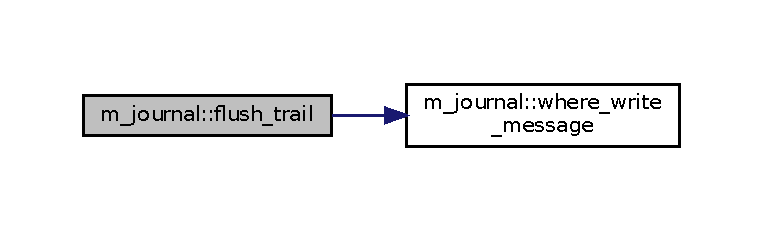
\includegraphics[width=350pt]{namespacem__journal_a24b891eded8ca585a6a72ab0eef7016c_cgraph}
\end{center}
\end{figure}
\mbox{\Hypertarget{namespacem__journal_a1b516ae6ba2da17e10847cf68d6833b1}\label{namespacem__journal_a1b516ae6ba2da17e10847cf68d6833b1}} 
\index{m\+\_\+journal@{m\+\_\+journal}!msg\+\_\+one@{msg\+\_\+one}}
\index{msg\+\_\+one@{msg\+\_\+one}!m\+\_\+journal@{m\+\_\+journal}}
\subsubsection{\texorpdfstring{msg\+\_\+one()}{msg\_one()}}
{\footnotesize\ttfamily character(len=\+:) function, allocatable m\+\_\+journal\+::msg\+\_\+one (\begin{DoxyParamCaption}\item[{class($\ast$), dimension(\+:), intent(in)}]{generic0,  }\item[{class($\ast$), dimension(\+:), intent(in), optional}]{generic1,  }\item[{class($\ast$), dimension(\+:), intent(in), optional}]{generic2,  }\item[{class($\ast$), dimension(\+:), intent(in), optional}]{generic3,  }\item[{class($\ast$), dimension(\+:), intent(in), optional}]{generic4,  }\item[{class($\ast$), dimension(\+:), intent(in), optional}]{generic5,  }\item[{class($\ast$), dimension(\+:), intent(in), optional}]{generic6,  }\item[{class($\ast$), dimension(\+:), intent(in), optional}]{generic7,  }\item[{class($\ast$), dimension(\+:), intent(in), optional}]{generic8,  }\item[{class($\ast$), dimension(\+:), intent(in), optional}]{generic9,  }\item[{logical, intent(in), optional}]{nospace }\end{DoxyParamCaption})\hspace{0.3cm}{\ttfamily [private]}}



References print\+\_\+generic().

Here is the call graph for this function\+:\nopagebreak
\begin{figure}[H]
\begin{center}
\leavevmode
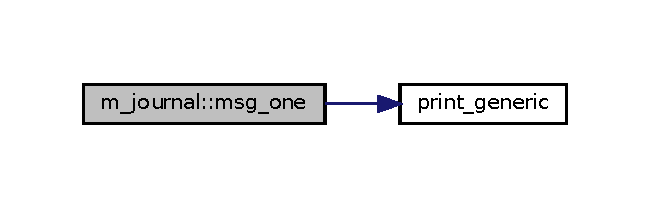
\includegraphics[width=312pt]{namespacem__journal_a1b516ae6ba2da17e10847cf68d6833b1_cgraph}
\end{center}
\end{figure}
\mbox{\Hypertarget{namespacem__journal_a7906bba242b412d6941f4b32233b7eca}\label{namespacem__journal_a7906bba242b412d6941f4b32233b7eca}} 
\index{m\+\_\+journal@{m\+\_\+journal}!msg\+\_\+scalar@{msg\+\_\+scalar}}
\index{msg\+\_\+scalar@{msg\+\_\+scalar}!m\+\_\+journal@{m\+\_\+journal}}
\subsubsection{\texorpdfstring{msg\+\_\+scalar()}{msg\_scalar()}}
{\footnotesize\ttfamily character(len=\+:) function, allocatable m\+\_\+journal\+::msg\+\_\+scalar (\begin{DoxyParamCaption}\item[{class($\ast$), intent(in), optional}]{generic0,  }\item[{class($\ast$), intent(in), optional}]{generic1,  }\item[{class($\ast$), intent(in), optional}]{generic2,  }\item[{class($\ast$), intent(in), optional}]{generic3,  }\item[{class($\ast$), intent(in), optional}]{generic4,  }\item[{class($\ast$), intent(in), optional}]{generic5,  }\item[{class($\ast$), intent(in), optional}]{generic6,  }\item[{class($\ast$), intent(in), optional}]{generic7,  }\item[{class($\ast$), intent(in), optional}]{generic8,  }\item[{class($\ast$), intent(in), optional}]{generic9,  }\item[{class($\ast$), intent(in), optional}]{generica,  }\item[{class($\ast$), intent(in), optional}]{genericb,  }\item[{class($\ast$), intent(in), optional}]{genericc,  }\item[{class($\ast$), intent(in), optional}]{genericd,  }\item[{class($\ast$), intent(in), optional}]{generice,  }\item[{class($\ast$), intent(in), optional}]{genericf,  }\item[{class($\ast$), intent(in), optional}]{genericg,  }\item[{class($\ast$), intent(in), optional}]{generich,  }\item[{class($\ast$), intent(in), optional}]{generici,  }\item[{class($\ast$), intent(in), optional}]{genericj,  }\item[{logical, intent(in), optional}]{nospace }\end{DoxyParamCaption})\hspace{0.3cm}{\ttfamily [private]}}



References print\+\_\+generic().

Here is the call graph for this function\+:\nopagebreak
\begin{figure}[H]
\begin{center}
\leavevmode
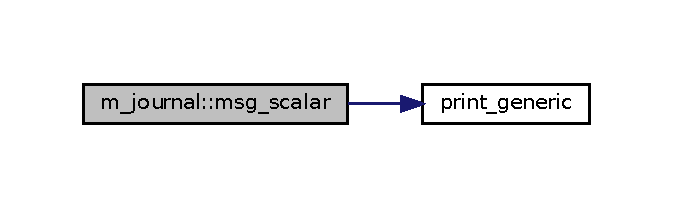
\includegraphics[width=323pt]{namespacem__journal_a7906bba242b412d6941f4b32233b7eca_cgraph}
\end{center}
\end{figure}
\mbox{\Hypertarget{namespacem__journal_a8388800481a5e7ca022b52cfc56b9daf}\label{namespacem__journal_a8388800481a5e7ca022b52cfc56b9daf}} 
\index{m\+\_\+journal@{m\+\_\+journal}!set\+\_\+stdout\+\_\+lun@{set\+\_\+stdout\+\_\+lun}}
\index{set\+\_\+stdout\+\_\+lun@{set\+\_\+stdout\+\_\+lun}!m\+\_\+journal@{m\+\_\+journal}}
\subsubsection{\texorpdfstring{set\+\_\+stdout\+\_\+lun()}{set\_stdout\_lun()}}
{\footnotesize\ttfamily subroutine m\+\_\+journal\+::set\+\_\+stdout\+\_\+lun (\begin{DoxyParamCaption}\item[{integer, intent(in)}]{iounit }\end{DoxyParamCaption})\hspace{0.3cm}{\ttfamily [private]}}



References stdout.

\mbox{\Hypertarget{namespacem__journal_a21238c3fc7731703c75eb39233ab529e}\label{namespacem__journal_a21238c3fc7731703c75eb39233ab529e}} 
\index{m\+\_\+journal@{m\+\_\+journal}!where\+\_\+write\+\_\+message@{where\+\_\+write\+\_\+message}}
\index{where\+\_\+write\+\_\+message@{where\+\_\+write\+\_\+message}!m\+\_\+journal@{m\+\_\+journal}}
\subsubsection{\texorpdfstring{where\+\_\+write\+\_\+message()}{where\_write\_message()}}
{\footnotesize\ttfamily subroutine m\+\_\+journal\+::where\+\_\+write\+\_\+message (\begin{DoxyParamCaption}\item[{character(len=$\ast$), intent(in)}]{where,  }\item[{character(len=$\ast$), intent(in)}]{msg }\end{DoxyParamCaption})\hspace{0.3cm}{\ttfamily [private]}}



References debug, last\+\_\+int, and stdout.

Here is the caller graph for this function\+:\nopagebreak
\begin{figure}[H]
\begin{center}
\leavevmode
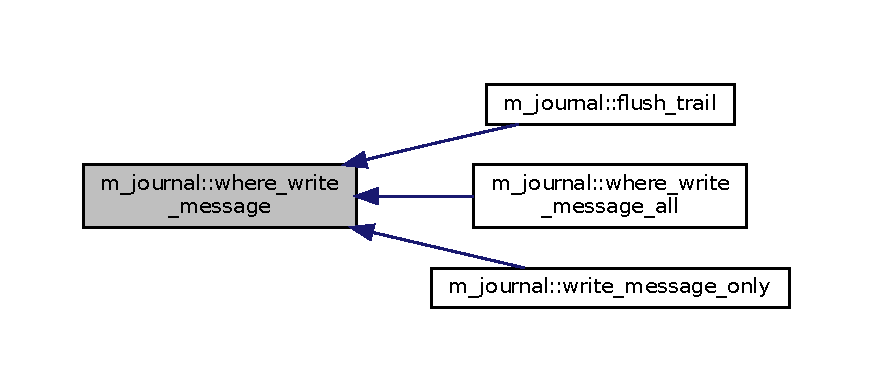
\includegraphics[width=350pt]{namespacem__journal_a21238c3fc7731703c75eb39233ab529e_icgraph}
\end{center}
\end{figure}
\mbox{\Hypertarget{namespacem__journal_a25d0f5da7f7e84e22ab0a583447412b1}\label{namespacem__journal_a25d0f5da7f7e84e22ab0a583447412b1}} 
\index{m\+\_\+journal@{m\+\_\+journal}!where\+\_\+write\+\_\+message\+\_\+all@{where\+\_\+write\+\_\+message\+\_\+all}}
\index{where\+\_\+write\+\_\+message\+\_\+all@{where\+\_\+write\+\_\+message\+\_\+all}!m\+\_\+journal@{m\+\_\+journal}}
\subsubsection{\texorpdfstring{where\+\_\+write\+\_\+message\+\_\+all()}{where\_write\_message\_all()}}
{\footnotesize\ttfamily subroutine m\+\_\+journal\+::where\+\_\+write\+\_\+message\+\_\+all (\begin{DoxyParamCaption}\item[{character(len=$\ast$), intent(in)}]{where,  }\item[{class($\ast$), intent(in)}]{g0,  }\item[{class($\ast$), intent(in), optional}]{g1,  }\item[{class($\ast$), intent(in), optional}]{g2,  }\item[{class($\ast$), intent(in), optional}]{g3,  }\item[{class($\ast$), intent(in), optional}]{g4,  }\item[{class($\ast$), intent(in), optional}]{g5,  }\item[{class($\ast$), intent(in), optional}]{g6,  }\item[{class($\ast$), intent(in), optional}]{g7,  }\item[{class($\ast$), intent(in), optional}]{g8,  }\item[{class($\ast$), intent(in), optional}]{g9,  }\item[{logical, intent(in), optional}]{nospace }\end{DoxyParamCaption})\hspace{0.3cm}{\ttfamily [private]}}



References where\+\_\+write\+\_\+message().

Here is the call graph for this function\+:\nopagebreak
\begin{figure}[H]
\begin{center}
\leavevmode
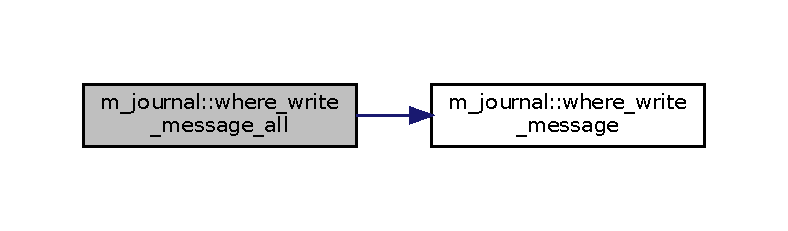
\includegraphics[width=350pt]{namespacem__journal_a25d0f5da7f7e84e22ab0a583447412b1_cgraph}
\end{center}
\end{figure}
\mbox{\Hypertarget{namespacem__journal_aa86511a7c388f9286c282f6fa933ab58}\label{namespacem__journal_aa86511a7c388f9286c282f6fa933ab58}} 
\index{m\+\_\+journal@{m\+\_\+journal}!write\+\_\+message\+\_\+only@{write\+\_\+message\+\_\+only}}
\index{write\+\_\+message\+\_\+only@{write\+\_\+message\+\_\+only}!m\+\_\+journal@{m\+\_\+journal}}
\subsubsection{\texorpdfstring{write\+\_\+message\+\_\+only()}{write\_message\_only()}}
{\footnotesize\ttfamily subroutine m\+\_\+journal\+::write\+\_\+message\+\_\+only (\begin{DoxyParamCaption}\item[{character(len=$\ast$), intent(in)}]{message }\end{DoxyParamCaption})\hspace{0.3cm}{\ttfamily [private]}}



References where\+\_\+write\+\_\+message().

Here is the call graph for this function\+:\nopagebreak
\begin{figure}[H]
\begin{center}
\leavevmode
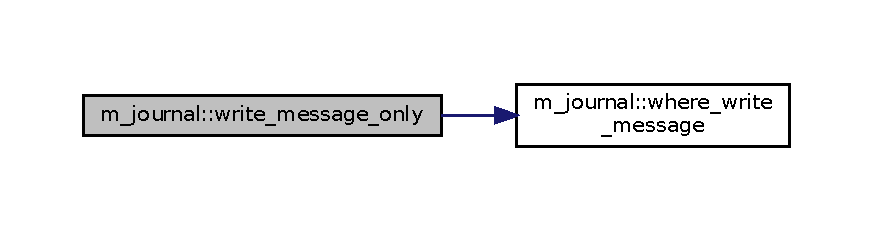
\includegraphics[width=350pt]{namespacem__journal_aa86511a7c388f9286c282f6fa933ab58_cgraph}
\end{center}
\end{figure}


\subsection{Variable Documentation}
\mbox{\Hypertarget{namespacem__journal_a6184fbcebdfa06f0a45ce4c699189b53}\label{namespacem__journal_a6184fbcebdfa06f0a45ce4c699189b53}} 
\index{m\+\_\+journal@{m\+\_\+journal}!debug@{debug}}
\index{debug@{debug}!m\+\_\+journal@{m\+\_\+journal}}
\subsubsection{\texorpdfstring{debug}{debug}}
{\footnotesize\ttfamily logical, save m\+\_\+journal\+::debug =.false.\hspace{0.3cm}{\ttfamily [private]}}

\mbox{\Hypertarget{namespacem__journal_a47e8e34dc4072b04101027394d688519}\label{namespacem__journal_a47e8e34dc4072b04101027394d688519}} 
\index{m\+\_\+journal@{m\+\_\+journal}!last\+\_\+int@{last\+\_\+int}}
\index{last\+\_\+int@{last\+\_\+int}!m\+\_\+journal@{m\+\_\+journal}}
\subsubsection{\texorpdfstring{last\+\_\+int}{last\_int}}
{\footnotesize\ttfamily integer, save m\+\_\+journal\+::last\+\_\+int =0\hspace{0.3cm}{\ttfamily [private]}}

\mbox{\Hypertarget{namespacem__journal_a664cf3fd85385b776d30ea589606ad1c}\label{namespacem__journal_a664cf3fd85385b776d30ea589606ad1c}} 
\index{m\+\_\+journal@{m\+\_\+journal}!stdout@{stdout}}
\index{stdout@{stdout}!m\+\_\+journal@{m\+\_\+journal}}
\subsubsection{\texorpdfstring{stdout}{stdout}}
{\footnotesize\ttfamily integer, save, private m\+\_\+journal\+::stdout =O\+U\+T\+P\+U\+T\+\_\+\+U\+N\+IT\hspace{0.3cm}{\ttfamily [private]}}


\hypertarget{namespacem__strings}{}\section{m\+\_\+strings Module Reference}
\label{namespacem__strings}\index{m\+\_\+strings@{m\+\_\+strings}}


\subsubsection*{N\+A\+ME}

M\+\_\+strings(3f) -\/ \mbox{[}M\+\_\+strings\+:I\+N\+T\+RO\mbox{]} Fortran string module \subsubsection*{D\+E\+S\+C\+R\+I\+P\+T\+I\+ON} 


\subsection*{Data Types}
\begin{DoxyCompactItemize}
\item 
interface \mbox{\hyperlink{interfacem__strings_1_1dble}{dble}}
\item 
interface \mbox{\hyperlink{interfacem__strings_1_1int}{int}}
\item 
interface \mbox{\hyperlink{interfacem__strings_1_1msg}{msg}}
\item 
interface \mbox{\hyperlink{interfacem__strings_1_1real}{real}}
\item 
interface \mbox{\hyperlink{interfacem__strings_1_1string__to__value}{string\+\_\+to\+\_\+value}}
\item 
interface \mbox{\hyperlink{interfacem__strings_1_1switch}{switch}}
\item 
interface \mbox{\hyperlink{interfacem__strings_1_1v2s}{v2s}}
\end{DoxyCompactItemize}
\subsection*{Functions/\+Subroutines}
\begin{DoxyCompactItemize}
\item 
logical function, public \mbox{\hyperlink{namespacem__strings_a5f96f66162f0f04d58b4f5dced8e82c6}{matchw}} (tame, wild)
\begin{DoxyCompactList}\small\item\em \subsubsection*{N\+A\+ME}

matchw(3f) -\/ \mbox{[}M\+\_\+strings\+:C\+O\+M\+P\+A\+RE\mbox{]} compare given string for match to pattern which may contain wildcard characters (L\+I\+C\+E\+N\+SE\+:PD) \end{DoxyCompactList}\item 
subroutine, public \mbox{\hyperlink{namespacem__strings_a3f0119fab962146c7656cad592dd9acd}{split}} (input\+\_\+line, array, delimiters, order, nulls)
\begin{DoxyCompactList}\small\item\em \subsubsection*{N\+A\+ME}

split(3f) -\/ \mbox{[}M\+\_\+strings\+:T\+O\+K\+E\+NS\mbox{]} parse string into an array using specified delimiters (L\+I\+C\+E\+N\+SE\+:PD) \end{DoxyCompactList}\item 
integer function, public \mbox{\hyperlink{namespacem__strings_aa3fc15a665eeff512b7f5269029f558d}{chomp}} (source\+\_\+string, token, delimiters)
\begin{DoxyCompactList}\small\item\em \subsubsection*{N\+A\+ME}

chomp(3f) -\/ \mbox{[}M\+\_\+strings\+:T\+O\+K\+E\+NS\mbox{]} Tokenize a string, consuming it one token per call (L\+I\+C\+E\+N\+SE\+:PD) \end{DoxyCompactList}\item 
subroutine, public \mbox{\hyperlink{namespacem__strings_a9890da826d63d6f04367887007611cb5}{delim}} (line, array, n, icount, ibegin, iterm, ilen, dlim)
\begin{DoxyCompactList}\small\item\em \subsubsection*{N\+A\+ME}

delim(3f) -\/ \mbox{[}M\+\_\+strings\+:T\+O\+K\+E\+NS\mbox{]} parse a string and store tokens into an array (L\+I\+C\+E\+N\+SE\+:PD) \subsubsection*{S\+Y\+N\+O\+P\+S\+IS}\end{DoxyCompactList}\item 
subroutine \mbox{\hyperlink{namespacem__strings_a818d715927dd61c1be6df5d2cdec4e4c}{crack\+\_\+cmd}} (cmd, old, new, ierr)
\begin{DoxyCompactList}\small\item\em \subsubsection*{N\+A\+ME}

replace(3f) -\/ \mbox{[}M\+\_\+strings\+:E\+D\+I\+T\+I\+NG\mbox{]} function globally replaces one substring for another in string (L\+I\+C\+E\+N\+SE\+:PD) \end{DoxyCompactList}\item 
character(len=\+:) function, allocatable, public \mbox{\hyperlink{namespacem__strings_ab5af73797bb08e7f654d39c9e8984ffe}{replace}} (targetline, old, new, ierr, cmd, range)
\item 
subroutine, public \mbox{\hyperlink{namespacem__strings_ab84a4b7c2be211433c2d1b435a87fa32}{substitute}} (targetline, old, new, ierr, start, end)
\begin{DoxyCompactList}\small\item\em \subsubsection*{N\+A\+ME}

substitute(3f) -\/ \mbox{[}M\+\_\+strings\+:E\+D\+I\+T\+I\+NG\mbox{]} subroutine globally substitutes one substring for another in string (L\+I\+C\+E\+N\+SE\+:PD) \end{DoxyCompactList}\item 
subroutine, public \mbox{\hyperlink{namespacem__strings_a1222f3b718f7637105bde330367925e1}{change}} (target\+\_\+string, cmd, ierr)
\begin{DoxyCompactList}\small\item\em \subsubsection*{N\+A\+ME}

change(3f) -\/ \mbox{[}M\+\_\+strings\+:E\+D\+I\+T\+I\+NG\mbox{]} change old string to new string with a directive like a line editor (L\+I\+C\+E\+N\+SE\+:PD) \end{DoxyCompactList}\item 
logical function, public \mbox{\hyperlink{namespacem__strings_aa53af9135873e241c487a75a7073bda1}{strtok}} (source\+\_\+string, itoken, token\+\_\+start, token\+\_\+end, delimiters)
\begin{DoxyCompactList}\small\item\em \subsubsection*{N\+A\+ME}

strtok(3f) -\/ \mbox{[}M\+\_\+strings\+:T\+O\+K\+E\+NS\mbox{]} Tokenize a string (L\+I\+C\+E\+N\+SE\+:PD) \subsubsection*{S\+Y\+N\+O\+P\+S\+IS}\end{DoxyCompactList}\item 
subroutine, public \mbox{\hyperlink{namespacem__strings_aec887410b018916a683fbb2ae529f8c5}{modif}} (C\+L\+I\+NE, M\+OD)
\begin{DoxyCompactList}\small\item\em \subsubsection*{N\+A\+ME}

modif(3f) -\/ \mbox{[}M\+\_\+strings\+:E\+D\+I\+T\+I\+NG\mbox{]} emulate the M\+O\+D\+I\+FY command from the line editor X\+E\+D\+IT (L\+I\+C\+E\+N\+SE\+:PD) \end{DoxyCompactList}\item 
elemental integer function, public \mbox{\hyperlink{namespacem__strings_aa1427d5dd673ff986236ba1732e693c1}{len\+\_\+white}} (string)
\begin{DoxyCompactList}\small\item\em \subsubsection*{N\+A\+ME}

len\+\_\+white(3f) -\/ \mbox{[}M\+\_\+strings\+:L\+E\+N\+G\+TH\mbox{]} get length of string trimmed of whitespace. (L\+I\+C\+E\+N\+SE\+:PD) \end{DoxyCompactList}\item 
character(len=\+:) function, allocatable, public \mbox{\hyperlink{namespacem__strings_a7030d33ae9e65d8cf2e2cb9332ffdac0}{crop}} (strin)
\begin{DoxyCompactList}\small\item\em \subsubsection*{N\+A\+ME}

crop(3f) -\/ \mbox{[}M\+\_\+strings\+:W\+H\+I\+T\+E\+S\+P\+A\+CE\mbox{]} trim leading blanks and trailing blanks from a string (L\+I\+C\+E\+N\+SE\+:PD) \end{DoxyCompactList}\item 
pure character(len=len(instr)) function, public \mbox{\hyperlink{namespacem__strings_aaee428861205782e002f5e7e8fb002f0}{transliterate}} (instr, old\+\_\+set, new\+\_\+set)
\begin{DoxyCompactList}\small\item\em \subsubsection*{N\+A\+ME}

transliterate(3f) -\/ \mbox{[}M\+\_\+strings\+:E\+D\+I\+T\+I\+NG\mbox{]} replace characters from old set with new set (L\+I\+C\+E\+N\+SE\+:PD) \end{DoxyCompactList}\item 
character(len=len(input)) function, public \mbox{\hyperlink{namespacem__strings_af155dcea0c0ccef21bb359040b673014}{rotate13}} (input)
\begin{DoxyCompactList}\small\item\em \subsubsection*{N\+A\+ME}

rotate13(3f) -\/ \mbox{[}M\+\_\+strings\mbox{]} apply trivial R\+O\+T13 encryption to a string (L\+I\+C\+E\+N\+SE\+:PD) \subsubsection*{S\+Y\+N\+O\+P\+S\+IS}\end{DoxyCompactList}\item 
pure character(len=\+:) function, allocatable, public \mbox{\hyperlink{namespacem__strings_a36c4cc6f83b736b4e337a1289694e3d6}{join}} (str, sep, trm, left, right)
\begin{DoxyCompactList}\small\item\em \subsubsection*{N\+A\+ME}

join(3f) -\/ \mbox{[}M\+\_\+strings\+:E\+D\+I\+T\+I\+NG\mbox{]} append C\+H\+A\+R\+A\+C\+T\+ER variable array into a single C\+H\+A\+R\+A\+C\+T\+ER variable with specified separator (L\+I\+C\+E\+N\+SE\+:PD) \end{DoxyCompactList}\item 
elemental character(len=len(string)) function, public \mbox{\hyperlink{namespacem__strings_ab3e5e7af9e9594fdb544f82736a26f17}{reverse}} (string)
\begin{DoxyCompactList}\small\item\em \subsubsection*{N\+A\+ME}

reverse(3f) -\/ \mbox{[}M\+\_\+strings\+:E\+D\+I\+T\+I\+NG\mbox{]} Return a string reversed (L\+I\+C\+E\+N\+SE\+:PD) \end{DoxyCompactList}\item 
elemental pure character(len=len(str)) function, public \mbox{\hyperlink{namespacem__strings_a3bd3b1de054c81fcc18b69afc369fb21}{upper\+\_\+quoted}} (str)
\begin{DoxyCompactList}\small\item\em \subsubsection*{N\+A\+ME}

upper\+\_\+quoted(3f) -\/ \mbox{[}M\+\_\+strings\+:C\+A\+SE\mbox{]} elemental function converts string to miniscule skipping strings quoted per Fortran syntax rules (L\+I\+C\+E\+N\+SE\+:PD) \end{DoxyCompactList}\item 
elemental pure character(len(str)) function, public \mbox{\hyperlink{namespacem__strings_a0953ac5c4d31339fdd8ec3acc9c3c915}{upper}} (str, begin, end)
\begin{DoxyCompactList}\small\item\em \subsubsection*{N\+A\+ME}

upper(3f) -\/ \mbox{[}M\+\_\+strings\+:C\+A\+SE\mbox{]} changes a string to uppercase (L\+I\+C\+E\+N\+SE\+:PD) \end{DoxyCompactList}\item 
elemental pure character(len(str)) function, public \mbox{\hyperlink{namespacem__strings_a3c7d4be9051206e4b2f72112f9fdc3b4}{lower}} (str, begin, end)
\begin{DoxyCompactList}\small\item\em \subsubsection*{N\+A\+ME}

lower(3f) -\/ \mbox{[}M\+\_\+strings\+:C\+A\+SE\mbox{]} changes a string to lowercase over specified range (L\+I\+C\+E\+N\+SE\+:PD) \end{DoxyCompactList}\item 
pure character(len=size(array)) function, private \mbox{\hyperlink{namespacem__strings_a9365ae5277199446d93fc5208be2e9a5}{a2s}} (array)
\begin{DoxyCompactList}\small\item\em \subsubsection*{N\+A\+ME}\end{DoxyCompactList}\item 
pure character(len=1) function, dimension(len(string)), private \mbox{\hyperlink{namespacem__strings_a5b05f337c8851871a4fb0b3cf56663cd}{s2a}} (string)
\item 
pure character(kind=c\+\_\+char, len=1) function, dimension(len\+\_\+trim(string)+1), public \mbox{\hyperlink{namespacem__strings_a9a3d38d8e7c4212d63487b9b46bec3b7}{s2c}} (string)
\begin{DoxyCompactList}\small\item\em \subsubsection*{N\+A\+ME}

s2c(3f) -\/ \mbox{[}M\+\_\+strings\+:A\+R\+R\+AY\mbox{]} convert character variable to array of characters with last element set to null (L\+I\+C\+E\+N\+SE\+:PD) \end{DoxyCompactList}\item 
character(len=\+:) function, allocatable, public \mbox{\hyperlink{namespacem__strings_a0a8c0c16a34208351523068686cb743b}{c2s}} (c\+\_\+string\+\_\+pointer)
\begin{DoxyCompactList}\small\item\em \subsubsection*{N\+A\+ME}

c2s(3f) -\/ \mbox{[}M\+\_\+strings\+:A\+R\+R\+AY\mbox{]} convert C string pointer to Fortran character string (L\+I\+C\+E\+N\+SE\+:PD) \end{DoxyCompactList}\item 
integer function, public \mbox{\hyperlink{namespacem__strings_a020dcca7f01d33eedf28b17518a22b69}{indent}} (line)
\begin{DoxyCompactList}\small\item\em \subsubsection*{N\+A\+ME}

indent(3f) -\/ \mbox{[}M\+\_\+strings\+:W\+H\+I\+T\+E\+S\+P\+A\+CE\mbox{]} count number of leading spaces in a string (L\+I\+C\+E\+N\+SE\+:PD) \end{DoxyCompactList}\item 
character(len=\+:) function, allocatable, public \mbox{\hyperlink{namespacem__strings_a791e24ceb690010fd42a6c1f48311b55}{visible}} (input)
\begin{DoxyCompactList}\small\item\em \subsubsection*{N\+A\+ME}

visible(3f) -\/ \mbox{[}M\+\_\+strings\+:N\+O\+N\+A\+L\+P\+HA\mbox{]} expand a string to control and meta-\/control representations (L\+I\+C\+E\+N\+SE\+:PD) \end{DoxyCompactList}\item 
character(len=\+:) function, allocatable, public \mbox{\hyperlink{namespacem__strings_a33b248107c1521272b55cda5c4077378}{expand}} (line, escape)
\begin{DoxyCompactList}\small\item\em \subsubsection*{N\+A\+ME}

expand(3f) -\/ \mbox{[}M\+\_\+strings\+:N\+O\+N\+A\+L\+P\+HA\mbox{]} expand C-\/like escape sequences (L\+I\+C\+E\+N\+SE\+:PD) \end{DoxyCompactList}\item 
subroutine, public \mbox{\hyperlink{namespacem__strings_a3bf44ac06a670f55830e17a6f1108b9c}{notabs}} (I\+N\+S\+TR, O\+U\+T\+S\+TR, I\+L\+EN)
\begin{DoxyCompactList}\small\item\em \subsubsection*{N\+A\+ME}

notabs(3f) -\/ \mbox{[}M\+\_\+strings\+:N\+O\+N\+A\+L\+P\+HA\mbox{]} expand tab characters (L\+I\+C\+E\+N\+SE\+:PD) \subsubsection*{S\+Y\+N\+O\+P\+S\+IS}\end{DoxyCompactList}\item 
pure character(len=\+:) function, allocatable, public \mbox{\hyperlink{namespacem__strings_a1cacb2e45c7e3d7ed4cc1b183c35f323}{adjustc}} (string, length)
\begin{DoxyCompactList}\small\item\em \subsubsection*{N\+A\+ME}

adjustc(3f) -\/ \mbox{[}M\+\_\+strings\+:W\+H\+I\+T\+E\+S\+P\+A\+CE\mbox{]} center text (L\+I\+C\+E\+N\+SE\+:PD) \end{DoxyCompactList}\item 
character(len=\+:) function, allocatable, public \mbox{\hyperlink{namespacem__strings_ad007f050abe3d142f4a7badbc4408685}{nospace}} (line)
\begin{DoxyCompactList}\small\item\em \subsubsection*{N\+A\+ME}

nospace(3f) -\/ \mbox{[}M\+\_\+strings\+:W\+H\+I\+T\+E\+S\+P\+A\+CE\mbox{]} remove all whitespace from input string (L\+I\+C\+E\+N\+SE\+:PD) \end{DoxyCompactList}\item 
character(len=\+:) function, allocatable, public \mbox{\hyperlink{namespacem__strings_aa67b36ec70dbad84672d3069882929c5}{stretch}} (line, length, pattern, suffix)
\begin{DoxyCompactList}\small\item\em \subsubsection*{N\+A\+ME}

stretch(3f) -\/ \mbox{[}M\+\_\+strings\+:L\+E\+N\+G\+TH\mbox{]} return string padded to at least specified length (L\+I\+C\+E\+N\+SE\+:PD) \end{DoxyCompactList}\item 
function, public \mbox{\hyperlink{namespacem__strings_ab20ba3a07833232eb3c67d4020a7fe64}{atleast}} (line, length, pattern)
\begin{DoxyCompactList}\small\item\em \subsubsection*{N\+A\+ME}

atleast(3f) -\/ \mbox{[}M\+\_\+strings\+:L\+E\+N\+G\+TH\mbox{]} return string padded to at least specified length (L\+I\+C\+E\+N\+SE\+:PD) \end{DoxyCompactList}\item 
character(len=length) function, public \mbox{\hyperlink{namespacem__strings_a378563bb49f128bf0cf9c9d2b1f34498}{lenset}} (line, length)
\begin{DoxyCompactList}\small\item\em \subsubsection*{N\+A\+ME}

lenset(3f) -\/ \mbox{[}M\+\_\+strings\+:L\+E\+N\+G\+TH\mbox{]} return string trimmed or padded to specified length (L\+I\+C\+E\+N\+SE\+:PD) \end{DoxyCompactList}\item 
character(len=\+:) function, allocatable, public \mbox{\hyperlink{namespacem__strings_aba5a8d7fc092b38d1939f37a13247c1e}{merge\+\_\+str}} (str1, str2, expr)
\begin{DoxyCompactList}\small\item\em \subsubsection*{N\+A\+ME}

merge\+\_\+str(3f) -\/ \mbox{[}M\+\_\+strings\+:L\+E\+N\+G\+TH\mbox{]} pads strings to same length and then calls M\+E\+R\+G\+E(3f) (L\+I\+C\+E\+N\+SE\+:PD) \end{DoxyCompactList}\item 
character(len=len(str)) function, public \mbox{\hyperlink{namespacem__strings_a929c032267cb990ad4991fab4aed1d57}{compact}} (str, char)
\begin{DoxyCompactList}\small\item\em \subsubsection*{N\+A\+ME}

compact(3f) -\/ \mbox{[}M\+\_\+strings\+:W\+H\+I\+T\+E\+S\+P\+A\+CE\mbox{]} converts contiguous whitespace to a single character (or nothing) (L\+I\+C\+E\+N\+SE\+:PD) \end{DoxyCompactList}\item 
elemental character(len=len(instr)) function, public \mbox{\hyperlink{namespacem__strings_a5d72fde097444c689f1822c5ad95e03d}{noesc}} (I\+N\+S\+TR)
\begin{DoxyCompactList}\small\item\em \subsubsection*{N\+A\+ME}

noesc(3f) -\/ \mbox{[}M\+\_\+strings\+:N\+O\+N\+A\+L\+P\+HA\mbox{]} convert non-\/printable characters to a space. (L\+I\+C\+E\+N\+SE\+:PD) \end{DoxyCompactList}\item 
subroutine, private \mbox{\hyperlink{namespacem__strings_a6b4babf586dc3586426b13e4bb0fb979}{a2r}} (chars, valu, ierr)
\begin{DoxyCompactList}\small\item\em \subsubsection*{N\+A\+ME}

string\+\_\+to\+\_\+value(3f) -\/ \mbox{[}M\+\_\+strings\+:N\+U\+M\+E\+R\+IC\mbox{]} subroutine returns numeric value from string (L\+I\+C\+E\+N\+SE\+:PD) \end{DoxyCompactList}\item 
subroutine, private \mbox{\hyperlink{namespacem__strings_aca902af295ede82fb0c45174bbfe6eef}{a2i}} (chars, valu, ierr)
\item 
subroutine, private \mbox{\hyperlink{namespacem__strings_a8a18024e04cc697243355de3d61e171c}{a2d}} (chars, valu, ierr, onerr)
\item 
doubleprecision function, public \mbox{\hyperlink{namespacem__strings_ae0e2fe7c93e581402a74a7b59e5bb07f}{s2v}} (chars, ierr, onerr)
\begin{DoxyCompactList}\small\item\em \subsubsection*{N\+A\+ME}

s2v(3f) -\/ \mbox{[}M\+\_\+strings\+:N\+U\+M\+E\+R\+IC\mbox{]} function returns doubleprecision numeric value from a string (L\+I\+C\+E\+N\+SE\+:PD) \end{DoxyCompactList}\item 
doubleprecision function \mbox{\hyperlink{namespacem__strings_a970d99e3a2ab426bb90d6ea90bcc588a}{dble\+\_\+s2v}} (chars)
\item 
\mbox{\hyperlink{interfacem__strings_1_1real}{real}} function \mbox{\hyperlink{namespacem__strings_aac80fa95c07cf00d5442a88962c5e6e9}{real\+\_\+s2v}} (chars)
\item 
integer function \mbox{\hyperlink{namespacem__strings_aa94164439fc7659e175cf639e7315c0d}{int\+\_\+s2v}} (chars)
\item 
integer function, dimension(\+:), allocatable \mbox{\hyperlink{namespacem__strings_a4e54d205168cab37d25119d74a9ead63}{ints\+\_\+s2v}} (chars)
\item 
\mbox{\hyperlink{interfacem__strings_1_1real}{real}} function, dimension(\+:), allocatable \mbox{\hyperlink{namespacem__strings_ac62b68d2aeb2b404a3340101f2cb7f84}{reals\+\_\+s2v}} (chars)
\item 
doubleprecision function, dimension(\+:), allocatable \mbox{\hyperlink{namespacem__strings_ab463f9b431dd817b7b509608ec823b0f}{dbles\+\_\+s2v}} (chars)
\item 
subroutine, public \mbox{\hyperlink{namespacem__strings_a5dcd73626c8909c12f8ea29028927a88}{value\+\_\+to\+\_\+string}} (gval, chars, length, err, \mbox{\hyperlink{namespacem__strings_afccf1e453a4315a639f133f2f7c0078b}{fmt}}, trimz)
\begin{DoxyCompactList}\small\item\em \subsubsection*{N\+A\+ME}

value\+\_\+to\+\_\+string(3f) -\/ \mbox{[}M\+\_\+strings\+:N\+U\+M\+E\+R\+IC\mbox{]} return numeric string from a numeric value (L\+I\+C\+E\+N\+SE\+:PD) \end{DoxyCompactList}\item 
character(len=\+:) function, allocatable, public \mbox{\hyperlink{namespacem__strings_a76a00e3ca7fb7c9b9cadcd484c6e3946}{v2s\+\_\+bug}} (gval)
\begin{DoxyCompactList}\small\item\em \subsubsection*{N\+A\+ME}

v2s(3f) -\/ \mbox{[}M\+\_\+strings\+:N\+U\+M\+E\+R\+IC\mbox{]} return numeric string from a numeric value (L\+I\+C\+E\+N\+SE\+:PD) \end{DoxyCompactList}\item 
character(len=\+:) function, allocatable, private \mbox{\hyperlink{namespacem__strings_a14715e071aea9030b4c68c22fa5a455d}{d2s}} (dvalue, \mbox{\hyperlink{namespacem__strings_afccf1e453a4315a639f133f2f7c0078b}{fmt}})
\item 
character(len=\+:) function, allocatable, private \mbox{\hyperlink{namespacem__strings_ab67ea90007b3f2eb308a5fe8d1cf0df1}{r2s}} (rvalue, \mbox{\hyperlink{namespacem__strings_afccf1e453a4315a639f133f2f7c0078b}{fmt}})
\item 
character(len=\+:) function, allocatable, private \mbox{\hyperlink{namespacem__strings_a76d3a650fbfec1f65d8fd81042347408}{i2s}} (ivalue, \mbox{\hyperlink{namespacem__strings_afccf1e453a4315a639f133f2f7c0078b}{fmt}})
\item 
character(len=\+:) function, allocatable, private \mbox{\hyperlink{namespacem__strings_a75aa4dfd0a231e2bcad03d26231a7c29}{l2s}} (lvalue, \mbox{\hyperlink{namespacem__strings_afccf1e453a4315a639f133f2f7c0078b}{fmt}})
\item 
integer function, public \mbox{\hyperlink{namespacem__strings_a2b6c57cbc52fc86d2f02d0936d3484af}{isnumber}} (string, \mbox{\hyperlink{interfacem__strings_1_1msg}{msg}}, verbose)
\begin{DoxyCompactList}\small\item\em \subsubsection*{N\+A\+ME}

isnumber(3f) -\/ \mbox{[}M\+\_\+strings\+:N\+U\+M\+E\+R\+IC\mbox{]} determine if a string represents a number (L\+I\+C\+E\+N\+SE\+:PD) \subsubsection*{S\+Y\+N\+O\+P\+S\+IS}\end{DoxyCompactList}\item 
subroutine, private \mbox{\hyperlink{namespacem__strings_aedbeefa963a63edc16b10e2a833eb609}{trimzeros\+\_\+}} (string)
\begin{DoxyCompactList}\small\item\em \subsubsection*{N\+A\+ME}

trimzeros\+\_\+(3fp) -\/ \mbox{[}M\+\_\+strings\+:N\+U\+M\+E\+R\+IC\mbox{]} Delete trailing zeros from numeric decimal string (L\+I\+C\+E\+N\+SE\+:PD) \subsubsection*{S\+Y\+N\+O\+P\+S\+IS}\end{DoxyCompactList}\item 
subroutine, public \mbox{\hyperlink{namespacem__strings_a81b4b7f4f301b9e17604adbcace58d0c}{listout}} (icurve\+\_\+lists, icurve\+\_\+expanded, inums\+\_\+out, ierr)
\begin{DoxyCompactList}\small\item\em \subsubsection*{N\+A\+ME}

listout(3f) -\/ \mbox{[}M\+\_\+strings\+:N\+U\+M\+E\+R\+IC\mbox{]} expand a list of numbers where negative numbers denote range ends (1 -\/10 means 1 thru 10) (L\+I\+C\+E\+N\+SE\+:PD) \end{DoxyCompactList}\item 
character(len=\+:) function, allocatable, public \mbox{\hyperlink{namespacem__strings_a3596a4ec755ac897a1dbc0b225d5266a}{quote}} (str, mode, clip)
\begin{DoxyCompactList}\small\item\em \subsubsection*{N\+A\+ME}

quote(3f) -\/ \mbox{[}M\+\_\+strings\+:Q\+U\+O\+T\+ES\mbox{]} add quotes to string as if written with list-\/directed input (L\+I\+C\+E\+N\+SE\+:PD) \subsubsection*{S\+Y\+N\+O\+P\+S\+IS}\end{DoxyCompactList}\item 
character(len=\+:) function, allocatable, public \mbox{\hyperlink{namespacem__strings_acb88c65d5df2d5b3e55df2d2dab57390}{unquote}} (quoted\+\_\+str, esc)
\begin{DoxyCompactList}\small\item\em \subsubsection*{N\+A\+ME}

unquote(3f) -\/ \mbox{[}M\+\_\+strings\+:Q\+U\+O\+T\+ES\mbox{]} remove quotes from string as if read with list-\/directed input (L\+I\+C\+E\+N\+SE\+:PD) \subsubsection*{S\+Y\+N\+O\+P\+S\+IS}\end{DoxyCompactList}\item 
character(len=\+:) function, allocatable, public \mbox{\hyperlink{namespacem__strings_a8d7007f0c34d7db4c004dac56e609b3f}{describe}} (ch)
\begin{DoxyCompactList}\small\item\em \subsubsection*{N\+A\+ME}

describe(3f) -\/ \mbox{[}M\+\_\+strings\mbox{]} returns a string describing the name of a single character (L\+I\+C\+E\+N\+SE\+:PD) \end{DoxyCompactList}\item 
subroutine, public \mbox{\hyperlink{namespacem__strings_abf6c760f5d15a306bd252337d0a5ba4d}{getvals}} (line, values, icount, ierr)
\begin{DoxyCompactList}\small\item\em \subsubsection*{N\+A\+ME}

getvals(3f) -\/ \mbox{[}M\+\_\+strings\+:N\+U\+M\+E\+R\+IC\mbox{]} read arbitrary number of R\+E\+AL values from a character variable up to size of V\+A\+L\+U\+E\+S() array (L\+I\+C\+E\+N\+SE\+:PD) \end{DoxyCompactList}\item 
subroutine, public \mbox{\hyperlink{namespacem__strings_af3767887ce5c2373a6d9061ea6664bfc}{string\+\_\+to\+\_\+values}} (line, iread, values, inums, delims, ierr)
\begin{DoxyCompactList}\small\item\em \subsubsection*{N\+A\+ME}

string\+\_\+to\+\_\+values(3f) -\/ \mbox{[}M\+\_\+strings\+:N\+U\+M\+E\+R\+IC\mbox{]} read a string representing numbers into a numeric array (L\+I\+C\+E\+N\+SE\+:PD) \end{DoxyCompactList}\item 
doubleprecision function, dimension(\+:), allocatable, public \mbox{\hyperlink{namespacem__strings_ad7fffe79559a666aa28e1ed598b8670f}{s2vs}} (string, \mbox{\hyperlink{namespacem__strings_a9890da826d63d6f04367887007611cb5}{delim}})
\begin{DoxyCompactList}\small\item\em \subsubsection*{N\+A\+ME}

s2vs(3f) -\/ \mbox{[}M\+\_\+strings\+:N\+U\+M\+E\+R\+IC\mbox{]} given a string representing numbers return a numeric array (L\+I\+C\+E\+N\+SE\+:PD) \end{DoxyCompactList}\item 
elemental logical function, public \mbox{\hyperlink{namespacem__strings_a267f2fde729a75496c82a64754a91e54}{isprint}} (onechar)
\item 
elemental logical function, public \mbox{\hyperlink{namespacem__strings_a84c80fdeeba0679488ed8ad8d37e53c5}{isgraph}} (onechar)
\item 
elemental logical function, public \mbox{\hyperlink{namespacem__strings_a5cf6d7fbd1b3ea17e37c6213c6ba0fdb}{isalpha}} (ch)
\item 
elemental logical function, public \mbox{\hyperlink{namespacem__strings_a9953d1e400bedceab6a06910c6cdf208}{isxdigit}} (ch)
\item 
elemental logical function, public \mbox{\hyperlink{namespacem__strings_a9f5f98a6c93e21618a16d98a5de2debc}{isdigit}} (ch)
\item 
elemental logical function, public \mbox{\hyperlink{namespacem__strings_aebb074d3971c0b93e39d1cfaa45658d8}{isblank}} (ch)
\item 
elemental logical function, public \mbox{\hyperlink{namespacem__strings_afb63e9fefbc04e4e9a2ec4df4334078c}{isascii}} (ch)
\item 
elemental logical function, public \mbox{\hyperlink{namespacem__strings_ab32380c29451e56395153155c1632d74}{isspace}} (ch)
\item 
elemental logical function, public \mbox{\hyperlink{namespacem__strings_a4821cb5a5c4024c9dc6dd159300034ca}{iscntrl}} (ch)
\item 
elemental logical function, public \mbox{\hyperlink{namespacem__strings_a8712164e1f5fd717bdea854a3f067619}{ispunct}} (ch)
\item 
pure elemental logical function, public \mbox{\hyperlink{namespacem__strings_ac98536a1b69026cd5373dfff489f7733}{isupper}} (ch)
\item 
elemental logical function, public \mbox{\hyperlink{namespacem__strings_a9de5290748f02f575f3b7b859ff074ed}{islower}} (ch)
\item 
elemental logical function, public \mbox{\hyperlink{namespacem__strings_ad8fd9bbf618bdba2c3ac9fb3c8174362}{isalnum}} (ch)
\begin{DoxyCompactList}\small\item\em \subsubsection*{N\+A\+ME}

isalnum,isalpha,iscntrl,isdigit,isgraph,islower, isprint,ispunct,isspace,isupper,isascii,isblank,isxdigit(3f) -\/ \mbox{[}M\+\_\+strings\+:C\+O\+M\+P\+A\+RE\mbox{]} test membership in subsets of A\+S\+C\+II set (L\+I\+C\+E\+N\+SE\+:PD) \end{DoxyCompactList}\item 
logical function, public \mbox{\hyperlink{namespacem__strings_a635ef6f1dd73400e7b339392886d6357}{base}} (x, b, y, a)
\begin{DoxyCompactList}\small\item\em \subsubsection*{N\+A\+ME}

base(3f) -\/ \mbox{[}M\+\_\+strings\+:B\+A\+SE\mbox{]} convert whole number string in base \mbox{[}2-\/36\mbox{]} to string in alternate base \mbox{[}2-\/36\mbox{]} (L\+I\+C\+E\+N\+SE\+:PD) \end{DoxyCompactList}\item 
logical function, public \mbox{\hyperlink{namespacem__strings_a3883dae1b85c2d4a09d2d7e46ff422ab}{decodebase}} (string, basein, out\+\_\+baseten)
\begin{DoxyCompactList}\small\item\em \subsubsection*{N\+A\+ME}\end{DoxyCompactList}\item 
logical function, public \mbox{\hyperlink{namespacem__strings_a3a022b64dc902dc6043e3f265ee78e38}{codebase}} (inval10, outbase, answer)
\begin{DoxyCompactList}\small\item\em \subsubsection*{N\+A\+ME}\end{DoxyCompactList}\item 
integer function \mbox{\hyperlink{namespacem__strings_aded6e43ae13ff21d76c1739f01a40a63}{todecimal}} (\mbox{\hyperlink{namespacem__strings_a635ef6f1dd73400e7b339392886d6357}{base}}, instr)
\item 
character(len=\+:) function, allocatable \mbox{\hyperlink{namespacem__strings_aa896d221112afb3dbc90eeca6075b282}{tobase}} (\mbox{\hyperlink{namespacem__strings_a635ef6f1dd73400e7b339392886d6357}{base}}, number)
\item 
character(len=\+:) function, dimension(\+:), allocatable, public \mbox{\hyperlink{namespacem__strings_afccf1e453a4315a639f133f2f7c0078b}{fmt}} (source\+\_\+string, length)
\begin{DoxyCompactList}\small\item\em \subsubsection*{N\+A\+ME}

fmt(3f) -\/ \mbox{[}M\+\_\+strings\+:T\+O\+K\+E\+NS\mbox{]} Tokenize a string, consuming it one token per call (L\+I\+C\+E\+N\+SE\+:PD) \end{DoxyCompactList}\item 
integer(kind=int8) function, public \mbox{\hyperlink{namespacem__strings_acc1854720186b8a5582a339d1cbb134b}{setbits8}} (string)
\item 
integer(kind=int16) function, public \mbox{\hyperlink{namespacem__strings_a536b90500130aa47bde4def7ecd5f6aa}{setbits16}} (string)
\item 
integer(kind=int32) function, public \mbox{\hyperlink{namespacem__strings_a44fd7db30f28fd30086eff1a59fbfa7e}{setbits32}} (string)
\item 
integer(kind=int64) function, public \mbox{\hyperlink{namespacem__strings_a3d005819ec07b086dbc6d1c197834142}{setbits64}} (string)
\item 
character(len=\+:) function, allocatable \mbox{\hyperlink{namespacem__strings_a926d1d9f529487149f4e0a1de8294122}{msg\+\_\+scalar}} (generic1, generic2, generic3, generic4, generic5, generic6, generic7, generic8, generic9, \mbox{\hyperlink{namespacem__strings_ad007f050abe3d142f4a7badbc4408685}{nospace}})
\begin{DoxyCompactList}\small\item\em \subsubsection*{N\+A\+ME}

msg(3f) -\/ \mbox{[}M\+\_\+strings\mbox{]} converts any standard scalar type to a string (L\+I\+C\+E\+N\+SE\+:PD) \subsubsection*{S\+Y\+N\+O\+P\+S\+IS}\end{DoxyCompactList}\item 
character(len=\+:) function, allocatable \mbox{\hyperlink{namespacem__strings_a52d27df9dcea52039c6feccb782ec4fd}{msg\+\_\+one}} (generic1, generic2, generic3, generic4, generic5, generic6, generic7, generic8, generic9, \mbox{\hyperlink{namespacem__strings_ad007f050abe3d142f4a7badbc4408685}{nospace}})
\end{DoxyCompactItemize}
\subsection*{Variables}
\begin{DoxyCompactItemize}
\item 
character, parameter, public \mbox{\hyperlink{namespacem__strings_a9de5098e31c6411a43323b1d7f19a886}{ascii\+\_\+nul}} = char(0)
\item 
character, parameter, public \mbox{\hyperlink{namespacem__strings_ae939ea755cfa377c5ed5f09ba8b0e923}{ascii\+\_\+bel}} = char(7)
\item 
character, parameter, public \mbox{\hyperlink{namespacem__strings_a6d4b461b6fba6d81e0cee7b6e579c77b}{ascii\+\_\+bs}} = char(8)
\item 
character, parameter, public \mbox{\hyperlink{namespacem__strings_a3fef6116790e59c99f48ea31a7b00133}{ascii\+\_\+ht}} = char(9)
\item 
character, parameter, public \mbox{\hyperlink{namespacem__strings_a4d65d248433f7c6ea3188c558f795c23}{ascii\+\_\+lf}} = char(10)
\item 
character, parameter, public \mbox{\hyperlink{namespacem__strings_a52761941cc3dba4a2ed922d1b7841c90}{ascii\+\_\+ff}} = char(12)
\item 
character, parameter, public \mbox{\hyperlink{namespacem__strings_a1f58b48efb41665079ced6de505a3b65}{ascii\+\_\+cr}} = char(13)
\item 
character, parameter, public \mbox{\hyperlink{namespacem__strings_a6e9a1f921d2bb4a14a9b50a3b8f96288}{ascii\+\_\+esc}} = char(27)
\end{DoxyCompactItemize}


\subsection{Detailed Description}
\subsubsection*{N\+A\+ME}

M\+\_\+strings(3f) -\/ \mbox{[}M\+\_\+strings\+:I\+N\+T\+RO\mbox{]} Fortran string module \subsubsection*{D\+E\+S\+C\+R\+I\+P\+T\+I\+ON}

The M\+\_\+strings(3fm) module is a collection of Fortran procedures that supplement the built-\/in intrinsic string routines. Routines for parsing, tokenizing, changing case, substituting new strings for substrings, locating strings with simple wildcard expressions, removing tabs and line terminators and other string manipulations are included.

M\+\_\+strings\+\_\+oop(3fm) is a companion module that provides an O\+OP interface to the M\+\_\+strings module.

\subsubsection*{S\+Y\+N\+O\+P\+S\+IS}

public entities\+:

use M\+\_\+strings, only \+: split,delim,chomp use M\+\_\+strings, only \+: substitute,change,modif,transliterate,reverse,replace,join use M\+\_\+strings, only \+: upper,lower,upper\+\_\+quoted use M\+\_\+strings, only \+: rotate13 use M\+\_\+strings, only \+: adjustc,compact,nospace,indent,crop,unquote,quote use M\+\_\+strings, only \+: len\+\_\+white,atleast,stretch,lenset,merge\+\_\+str use M\+\_\+strings, only \+: switch,s2c,c2s use M\+\_\+strings, only \+: noesc,notabs,expand,uc,visible use M\+\_\+strings, only \+: \mbox{\hyperlink{interfacem__strings_1_1string__to__value}{string\+\_\+to\+\_\+value}},string\+\_\+to\+\_\+values,s2v,s2vs,value\+\_\+to\+\_\+string,\mbox{\hyperlink{interfacem__strings_1_1v2s}{v2s}},msg use M\+\_\+strings, only \+: listout,getvals use M\+\_\+strings, only \+: matchw use M\+\_\+strings, only \+: fmt use M\+\_\+strings, only \+: base, decodebase, codebase use M\+\_\+strings, only \+: isalnum, isalpha, iscntrl, isdigit, isgraph, islower, isprint, ispunct, isspace, isupper, isascii, isblank, isxdigit

T\+O\+K\+E\+NS

split subroutine parses string using specified delimiter characters and stores tokens into an array delim subroutine parses string using specified delimiter characters and store tokens into an array chomp function consumes input line as it returns next token in a string using specified delimiters fmt convert a string into a paragraph

E\+D\+I\+T\+I\+NG

substitute subroutine non-\/recursively globally replaces old substring with new substring replace function non-\/recursively globally replaces old substring with new substring using allocatable string (version of substitute(3f) without limitation on length of output string) change subroutine non-\/recursively globally replaces old substring with new substring with a directive like line editor modif subroutine modifies a string with a directive like the X\+E\+D\+IT line editor M\+O\+D\+I\+FY command transliterate replace characters found in set one with characters from set two reverse reverse character order in a string join join an array of C\+H\+A\+R\+A\+C\+T\+ER variables with specified separator rotate13 apply trivial encryption algorithm R\+O\+T13 to a string

C\+A\+SE

upper function converts string to uppercase lower function converts string to miniscule upper function converts string to uppercase skipping strings quoted per Fortran rules

W\+H\+I\+TE S\+P\+A\+CE

adjustc elemental function centers text within the length of the input string compact left justify string and replace duplicate whitespace with single characters or nothing nospace function replaces whitespace with nothing indent find number of leading spaces crop function trims leading and trailing spaces

Q\+U\+O\+T\+ES

unquote remove quotes from string as if read with list-\/directed input quote add quotes to string as if written with list-\/directed input

S\+T\+R\+I\+NG L\+E\+N\+G\+TH

len\+\_\+white find location of last non-\/whitespace character lenset return a string of specified length atleast return a string of at least specified length stretch return a string of at least specified length with suffix merge\+\_\+str make strings of equal length and then call M\+E\+R\+G\+E(3f) intrinsic

C\+H\+A\+R\+A\+C\+T\+ER A\+R\+R\+AY V\+E\+R\+S\+US S\+T\+R\+I\+NG

switch switch between a string and an array of single characters s2c convert string to array of single characters and add null terminator for passing to C c2s convert null-\/terminated array of single characters to string for converting strings returned from C

N\+O\+N\+A\+L\+P\+HA

noesc convert non-\/printable A\+S\+C\+I\+I8 characters to a space notabs convert tabs to spaces while maintaining columns, assuming tabs are set every 8 characters expand expand escape sequences in a string visible expand escape sequences in a string to control and meta-\/control representations

N\+U\+M\+E\+R\+IC S\+T\+R\+I\+N\+GS

\mbox{\hyperlink{interfacem__strings_1_1string__to__value}{string\+\_\+to\+\_\+value}} generic subroutine returns numeric value (R\+E\+AL, D\+O\+U\+B\+L\+E\+P\+R\+E\+C\+I\+S\+I\+ON, I\+N\+T\+E\+G\+ER) from string string\+\_\+to\+\_\+values subroutine reads an array of numbers from a string getvals subroutine reads a relatively arbitrary number of values from a string using list-\/directed read s2v function returns D\+O\+U\+B\+L\+E\+P\+R\+E\+C\+I\+S\+I\+ON numeric value from string s2vs function returns a D\+O\+U\+B\+L\+E\+P\+R\+E\+C\+I\+S\+I\+ON array of numbers from a string msg append the values of up to nine values into a string

value\+\_\+to\+\_\+string generic subroutine returns string given numeric value (R\+E\+AL, D\+O\+U\+B\+L\+E\+P\+R\+E\+C\+I\+S\+I\+ON, I\+N\+T\+E\+G\+ER, L\+O\+G\+I\+C\+AL ) \mbox{\hyperlink{interfacem__strings_1_1v2s}{v2s}} generic function returns string from numeric value (R\+E\+AL, D\+O\+U\+B\+L\+E\+P\+R\+E\+C\+I\+S\+I\+ON, I\+N\+T\+E\+G\+ER ) listout expand a list of numbers where negative numbers denote range ends (1 -\/10 means 1 thru 10) isnumber determine if string represents a number

C\+H\+A\+R\+A\+C\+T\+ER T\+E\+S\+TS

matchw compares given string for match to pattern which may contain wildcard characters

o isalnum returns .true. if character is a letter or digit o isalpha returns .true. if character is a letter and .false. otherwise o iscntrl returns .true. if character is a delete character or ordinary control character o isdigit returns .true. if character is a digit (0,1,...,9) and .false. otherwise o isgraph returns .true. if character is a printable character except a space is considered non-\/printable o islower returns .true. if character is a miniscule letter (a-\/z) o isprint returns .true. if character is an A\+S\+C\+II printable character o ispunct returns .true. if character is a printable punctuation character o isspace returns .true. if character is a null, space, tab, carriage return, new line, vertical tab, or formfeed o isupper returns .true. if character is an uppercase letter (A-\/Z) o isascii returns .true. if the character is in the range char(0) to char(127) o isblank returns .true. if character is a blank character (space or horizontal tab. o isxdigit returns .true. if character is a hexadecimal digit (0-\/9, a-\/f, or A-\/F).

B\+A\+SE C\+O\+N\+V\+E\+R\+S\+I\+ON

base convert whole number string in base \mbox{[}2-\/36\mbox{]} to string in alternate base \mbox{[}2-\/36\mbox{]} codebase convert whole number string in base \mbox{[}2-\/36\mbox{]} to base 10 number decodebase convert whole number in base 10 to string in base \mbox{[}2-\/36\mbox{]}

M\+I\+S\+C\+E\+L\+L\+A\+N\+E\+O\+US

describe returns a string describing the name of a single character

\begin{DoxyVerb}INTRINSICS

The M_strings(3fm) module supplements and works in combination with
the Fortran built-in intrinsics. Stand-alone
Fortran lets you access the characters in a string using ranges
much like they are character arrays, assignment, comparisons with
standard operators, supports dynamically allocatable strings and
supports concatenation using the // operator, as well as a number
of intrinsic string routines:

    adjustl             Left adjust a string
    adjustr             Right adjust a string
    index               Position of a substring within a string
    repeat              Repeated string concatenation
    scan                Scan a string for the presence of a set of characters
    trim                Remove trailing blank characters of a string
    verify              Scan a string for the absence of a set of characters
    len                 It returns the length of a character string
    achar               converts an integer into a character
    iachar              converts a character into an integer
    len_trim            finds length of string with trailing spaces ignored
    new_line            Newline character
    selected_char_kind  Choose character kind
    lge                 Lexical greater than or equal
    lgt                 Lexical greater than
    lle                 Lexical less than or equal
    llt                 Lexical less than

OOPS INTERFACE

The M_strings_oop(3fm) module (included with the M_strings(3fm)
module) provides an OOP (Object-Oriented Programming) interface
to the M_strings(3fm) module; as described in the example program
OBJECT_ORIENTED shown below...
\end{DoxyVerb}


\subsubsection*{S\+EE A\+L\+SO}

\begin{DoxyVerb}There are additional routines in other GPF modules for working with
expressions (M_calculator), time strings (M_time), random strings
(M_random, M_uuid), lists (M_list), and interfacing with the C regular
expression library (M_regex).
\end{DoxyVerb}


\subsubsection*{E\+X\+A\+M\+P\+L\+ES}

Each of the procedural functions includes an example program in the corresponding man(1) page for the function. The object-\/oriented interface does not have individual man(1) pages, but is instead demonstrated using the following example program\+: \begin{DoxyVerb}program demo_M_strings
!
! This is an example using the object-oriented class/type model
! defined in M_strings_oop
! This is essentially the same functionality as the procedures
! combined with several Fortran intrinsics and overloaded operators
!
use M_strings_oop,only : string, p
implicit none
TYPE(string) :: str1
TYPE(string) :: str2
TYPE(string) :: str3
TYPE(string) :: str4
!==============================================================================
  write(*,*)'exercise the M_STRING_OOP module interface'
  ! draw a break line in the output
  write(*,*)repeat('=',78)
  write(*,*)'Call methods of type(STRING)'
  ! define TYPE(STRING) with constructor
  str2=string('   This  is  a  String!       ')
  str4=string(' a  String ')
  write(*,*)repeat('=',78)
  ! print members of type
  write(*,101)'str2%str is ................ ',str2%str
  ! same as intrinsic LEN()
  write(*,202)'len ........................ ',str2%len()
  ! same as intrinsic INDEX()
  write(*,202)'len_trim ................... ',str2%len_trim()
  ! same as intrinsic INDEX()
  write(*,202)'index("is")................. ',str2%index("is")
  ! same as intrinsic INDEX()
  write(*,202)'index("is",back=.T.) ....... ',str2%index("is",back=.TRUE.)
  ! output TYPE(STRING) with %str all uppercase
  write(*,101)'upper ...................... ',p(str2%upper())
  ! output TYPE(STRING) with %str all miniscule
  write(*,101)'lower ...................... ',p(str2%lower())
  ! output TYPE(STRING) with %str reversed
  write(*,101)'reverse .................... ',p(str2%reverse())
  ! same as intrinsic ADJUSTL()
  write(*,101)'adjustl .................... ',p(str2%adjustl())
  ! same as intrinsic ADJUSTR()
  write(*,101)'adjustr .................... ',p(str2%adjustr())
  ! center string in current string length
  write(*,101)'adjustc .................... ',p(str2%adjustc())
  ! center string in string length of NN
  write(*,101)'adjustc(49) ................ ',p(str2%adjustc(49))
  ! force %str to be NN characters long
  write(*,101)'lenset(49) ................. ',p(str2%lenset(49))
  ! same as intrinsic TRIM()
  write(*,101)'trim ....................... ',p(str2%trim())
  ! trim leading and trailing spaces
  write(*,101)'crop ....................... ',p(str2%crop())
  ! calls M_strings procedure SUBSTITUTE()
  write(*,101)'substitute("This","Here") .. ',p(str2%substitute("This","Here"))
  ! calls M_strings procedure COMPACT()
  write(*,101)'compact .................... ',p(str2%compact())
  write(*,101)'compact("") ................ ',p(str2%compact(""))
  write(*,101)'compact(":") ............... ',p(str2%compact(":"))
  ! calls M_strings procedure TRANSLITERATE()
  write(*,101)'transliterate("aei","VWX") . ',p(str2%transliterate("aei","VWX"))
  write(*,101)'transliterate("aeiou"," ") . ',p(str2%transliterate("aeiou"," "))
  write(*,101)'transliterate("aeiou","") .. ',p(str2%transliterate("aeiou",""))
  write(*,101)'transliterate(" aeiou","") . ',p(str2%transliterate(" aeiou",""))
  ! calls M_strings procedure SWITCH()
  write(*,404)'chars .................... . ',str4%chars()

  write(*,*)repeat('=',78)
  str2%str='\t\tSome tabs\t   x\bX '
  write(*,101)'str2%str ................... ',str2%str
  write(*,101)'expand ..................... ',p(str2%expand())
  str2=str2%expand()
  ! calls M_strings procedure NOTABS()
  write(*,101)'notabs ..................... ',p(str2%notabs())
  ! calls M_strings procedure NOESC()
  write(*,101)'noesc ...................... ',p(str2%noesc())

  write(*,*)repeat('=',78)
  write(*,*)'Casting to numeric variables'
  str3=string('   12.345678901234567e1        ')
  write(*,101)'str3%str ................... ',str3%str
  ! calls M_strings procedure STRING_TO_VALUE()
  write(*,*)'int  ....................... ', str3%int()
  ! calls M_strings procedure STRING_TO_VALUE()
  write(*,*)'real ....................... ', str3%real()
  ! calls M_strings procedure STRING_TO_VALUE()
  write(*,*)'dble ....................... ', str3%dble()

  write(*,*)repeat('=',78)
  write(*,*)'Matching simple globbing patterns'
  str3=string('   12.345678901234567e1        ')
  str3=string('Four score and seven years ago')
  write(*,101)'str3%str ................... ',str3%str
  ! calls M_strings procedure MATCHW
  write(*,*)'match("Fo*") ............... ', str3%match("Fo*")
  ! calls M_strings procedure MATCHW
  write(*,*)'match("and") ............... ', str3%match("and")
  ! calls M_strings procedure MATCHW
  write(*,*)'match("*and*") ............. ', str3%match("*and*")

  101 format(1x,a,"[",a,"]")
  202 format(1x,a,i0)
  303 format(1x,*(l3))
  404 format(1x,a,*("[",a1,"]":))

  write(*,*)repeat('=',78)
  write(*,*)'OVERLOADED OPERATORS (add and subtract,return TYPE(STRING))'
  str1%str='123.456'
  str2%str='AaBbCcDdEeFfGgHhIiJj AaBbCcDdEeFfGgHhIiJj'
  write(*,101)'str1%str ................... ',str1%str
  write(*,101)'str2%str ................... ',str2%str
  write(*,*)'str1 + str2 ................ ',p(str1 + str2)
  ! a string that looks like a numeric value can have a value added
  write(*,*)'str1 + 20000 ............... ',p(str1 +20000)
  write(*,*)'str1 - 20.0 ................ ',p(str1 -20.0)
  write(*,*)'str2 - "Aa" (removes ALL) .. ',p(str2 - 'Aa')

  write(*,*)repeat('=',78)
  write(*,*)'OVERLOADED OPERATORS (multiply,return TYPE(STRING))'
  str1%str='AaBbCcDdEeFfGgHhIiJj'
  write(*,101)'str1%str ................... ',str1%str
  write(*,*)'str1 * 3 ................... ',p(str1 * 3)

  write(*,*)repeat('=',78)
  write(*,*)'OVERLOADED OPERATORS (//,return TYPE(STRING))'
  str1%str='String one:'
  str2%str='String two:'
  write(*,101)'str1%str ................... ',str1%str
  write(*,101)'str2%str ................... ',str2%str
  write(*,*)'str1 // str2 ................ ',p(str1 // str2)
  ! numeric values are converted to strings
  write(*,*)'str1 // 20000 ............... ',p(str1 // 20000)
  write(*,*)'str1 // 20.0 ................ ',p(str1 // 20.0)

  write(*,*)repeat('=',78)
  write(*,*)'OVERLOADED OPERATORS (logical comparisons,return logical)'
  ! NOTE: comparisons are performed on the character variable members
  !       of the type(string)
  str1%str='abcdefghij'
  str2%str='klmnopqrst'
  write(*,101)'str1%str ................... ',str1%str
  write(*,101)'str2%str ................... ',str2%str
  write(*,*)': EQ LT GT LE GE NE'
  write(*,*)'compare str1 to str1'
  write(*,303)str1.eq.str1  ,str1.lt.str1  ,str1.gt.str1  ,str1.le.str1 &
             & ,str1.ge.str1  ,str1.ne.str1
  write(*,*)'compare str1 to str2'
  write(*,303)str1.eq.str2  ,str1.lt.str2  ,str1.gt.str2  ,str1.le.str2 &
             & ,str1.ge.str2  ,str1.ne.str2
  write(*,*)'compare str2 to str1'
  write(*,303)str2.eq.str1  ,str2.lt.str1  ,str2.gt.str1  ,str2.le.str1 &
             & ,str2.ge.str1  ,str2.ne.str1

  write(*,*)repeat('=',78)

end program demo_M_strings
\end{DoxyVerb}


Expected output \begin{DoxyVerb}exercise the M_STRING_OOP module interface
=============================================================================
Call methods of type(STRING)
=============================================================================
str2%str is ................ [   This  is  a  String!             ]
len ........................ 36
len_trim ................... 23
index("is")................. 6
index("is",back=.T.) ....... 10
upper ...................... [   THIS  IS  A  STRING!             ]
lower ...................... [   this  is  a  string!             ]
reverse .................... [             !gnirtS  a  si  sihT   ]
adjustl .................... [This  is  a  String!                ]
adjustr .................... [                This  is  a  String!]
adjustc .................... [        This  is  a  String!        ]
adjustc(49) ................ [              This  is  a  String!               ]
lenset(49) ................. [   This  is  a  String!                          ]
trim ....................... [   This  is  a  String!]
crop ....................... [This  is  a  String!]
substitute("This","Here") .. [   Here  is  a  String!             ]
compact .................... [This is a String!]
compact("") ................ [ThisisaString!]
compact(":") ............... [This:is:a:String!]
transliterate("aei","VWX") . [   ThXs  Xs  V  StrXng!             ]
transliterate("aeiou"," ") . [   Th s   s     Str ng!             ]
transliterate("aeiou","") .. [   Ths  s    Strng!                 ]
transliterate(" aeiou","") . [ThssStrng!                          ]
chars .................... . [ ][a][ ][s][t][r][i][n][g][ ]
=============================================================================
str2%str ................... [\t\tSome tabs\t   x\bX ]
expand ..................... [         Some tabs          x   X]
notabs ..................... [                Some tabs          x    X]
noesc ...................... [  Some tabs    x X]
=============================================================================
Casting to numeric variables
str3%str ................... [   12.345678901234567e1        ]
int  .......................          123
real .......................    123.456787
dble .......................    123.45678901234567
=============================================================================
Matching simple globbing patterns
str3%str ................... [Four score and seven years ago]
match("Fo*") ...............  T
match("and") ...............  F
match("*and*") .............  T
==============================================================================
OVERLOADED OPERATORS (add and subtract, return TYPE(STRING))
str1%str ................... [123.456]
str2%str ................... [AaBbCcDdEeFfGgHhIiJj AaBbCcDdEeFfGgHhIiJj]
str1 + str2 ................ 123.456 AaBbCcDdEeFfGgHhIiJj AaBbCcDdEeFfGgHhIiJj
str1 + 20000 ............... 20123.455999999998
str1 - 20.0 ................ -103.456
str2 - "Aa" (removes ALL) .. BbCcDdEeFfGgHhIiJj BbCcDdEeFfGgHhIiJj
=============================================================================
OVERLOADED OPERATORS (multiply, return TYPE(STRING))
str1%str ................... [AaBbCcDdEeFfGgHhIiJj]
str1 * 3 ................... AaBbCcDdEeFfGgHhIiJjAaBbCcDdEeFfGgHhIiJjAaBbCcDdEeFfGgHhIiJj
=============================================================================
OVERLOADED OPERATORS (//, return TYPE(STRING))
str1%str ................... [String one:]
str2%str ................... [String two:]
str1 // str2 ................ String one:String two:
str1 // 20000 ............... String one:20000
str1 // 20.0 ................ String one:20.0
=============================================================================
OVERLOADED OPERATORS (logical comparisons, return logical)
str1%str ................... [abcdefghij]
str2%str ................... [klmnopqrst]
: EQ LT GT LE GE NE
compare str1 to str1
:  T  F  F  T  T  F
compare str1 to str2
:  F  T  F  T  F  T
compare str2 to str1
:  F  F  T  F  T  T
\end{DoxyVerb}
 ============================================================================= 

\subsection{Function/\+Subroutine Documentation}
\mbox{\Hypertarget{namespacem__strings_a8a18024e04cc697243355de3d61e171c}\label{namespacem__strings_a8a18024e04cc697243355de3d61e171c}} 
\index{m\+\_\+strings@{m\+\_\+strings}!a2d@{a2d}}
\index{a2d@{a2d}!m\+\_\+strings@{m\+\_\+strings}}
\subsubsection{\texorpdfstring{a2d()}{a2d()}}
{\footnotesize\ttfamily subroutine, private m\+\_\+strings\+::a2d (\begin{DoxyParamCaption}\item[{character(len=$\ast$), intent(in)}]{chars,  }\item[{doubleprecision, intent(out)}]{valu,  }\item[{integer, intent(out)}]{ierr,  }\item[{class($\ast$), intent(in), optional}]{onerr }\end{DoxyParamCaption})\hspace{0.3cm}{\ttfamily [private]}}



References decodebase(), fmt(), and substitute().

Here is the call graph for this function\+:\nopagebreak
\begin{figure}[H]
\begin{center}
\leavevmode
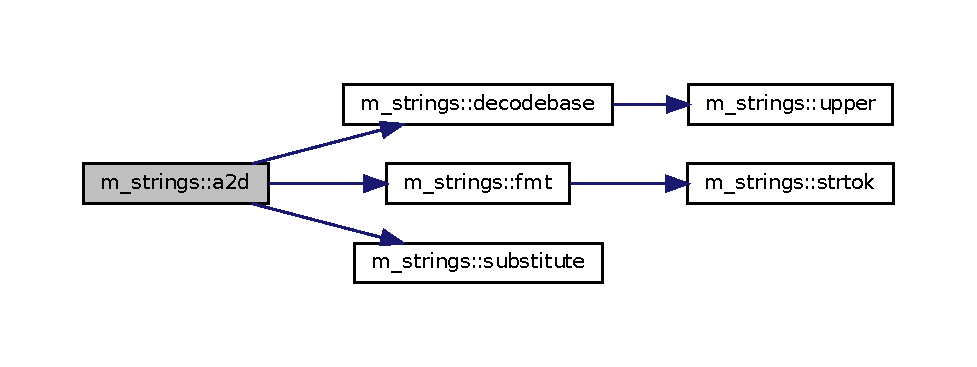
\includegraphics[width=350pt]{namespacem__strings_a8a18024e04cc697243355de3d61e171c_cgraph}
\end{center}
\end{figure}
Here is the caller graph for this function\+:\nopagebreak
\begin{figure}[H]
\begin{center}
\leavevmode
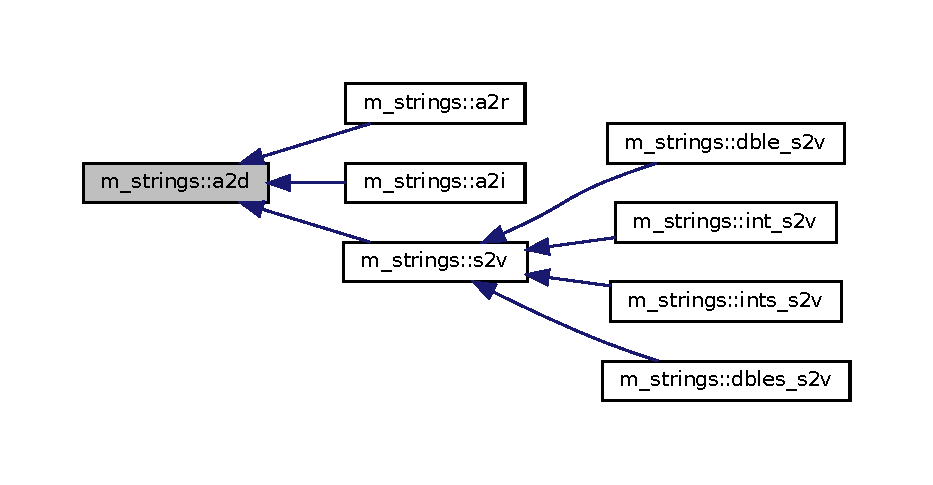
\includegraphics[width=350pt]{namespacem__strings_a8a18024e04cc697243355de3d61e171c_icgraph}
\end{center}
\end{figure}
\mbox{\Hypertarget{namespacem__strings_aca902af295ede82fb0c45174bbfe6eef}\label{namespacem__strings_aca902af295ede82fb0c45174bbfe6eef}} 
\index{m\+\_\+strings@{m\+\_\+strings}!a2i@{a2i}}
\index{a2i@{a2i}!m\+\_\+strings@{m\+\_\+strings}}
\subsubsection{\texorpdfstring{a2i()}{a2i()}}
{\footnotesize\ttfamily subroutine, private m\+\_\+strings\+::a2i (\begin{DoxyParamCaption}\item[{character(len=$\ast$), intent(in)}]{chars,  }\item[{integer, intent(out)}]{valu,  }\item[{integer, intent(out)}]{ierr }\end{DoxyParamCaption})\hspace{0.3cm}{\ttfamily [private]}}



References a2d().

Here is the call graph for this function\+:\nopagebreak
\begin{figure}[H]
\begin{center}
\leavevmode
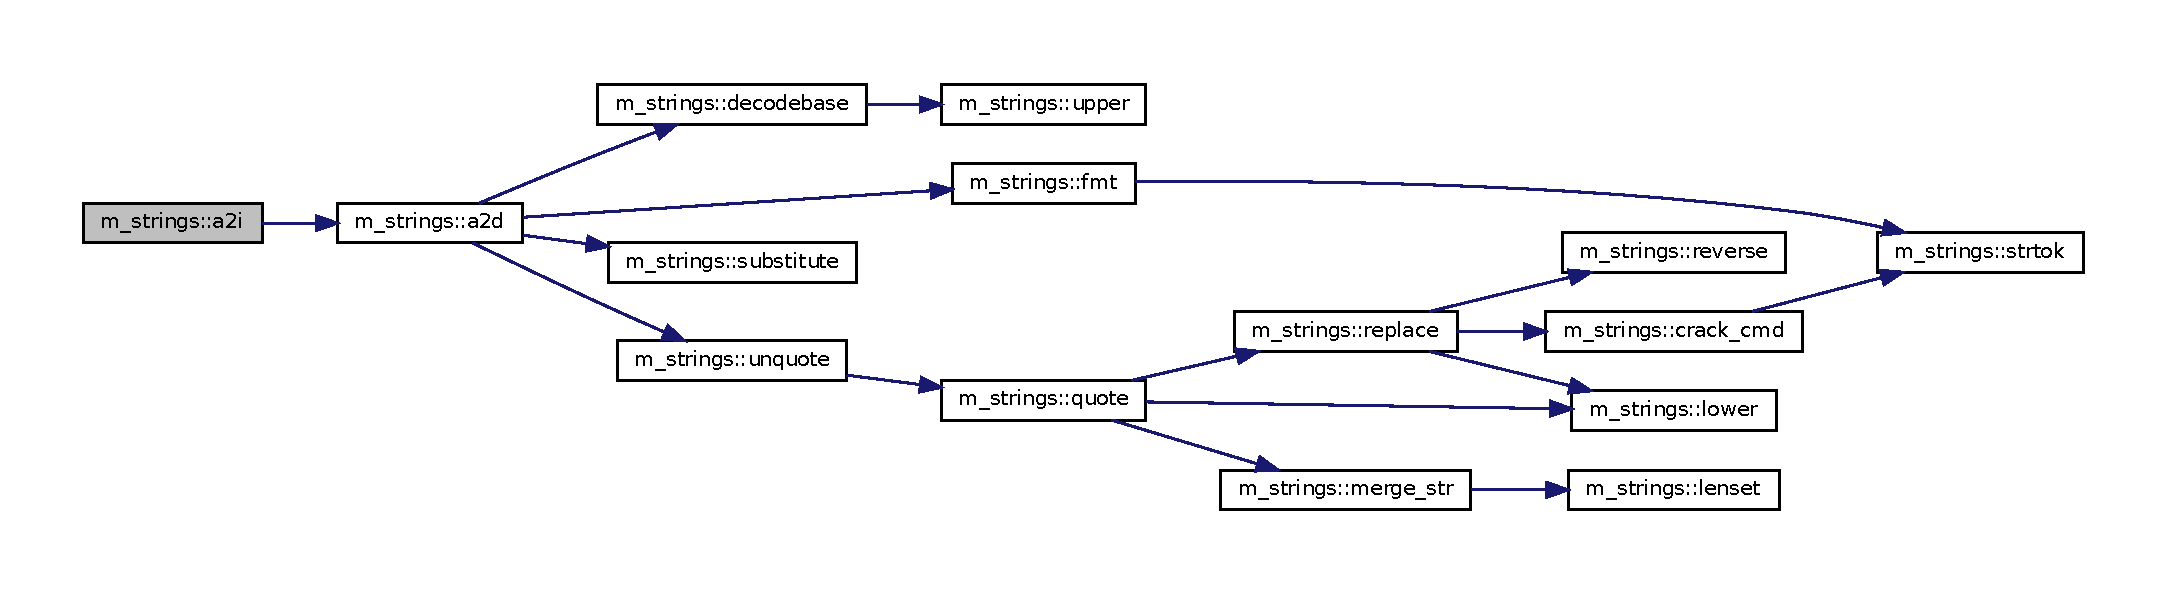
\includegraphics[width=350pt]{namespacem__strings_aca902af295ede82fb0c45174bbfe6eef_cgraph}
\end{center}
\end{figure}
\mbox{\Hypertarget{namespacem__strings_a6b4babf586dc3586426b13e4bb0fb979}\label{namespacem__strings_a6b4babf586dc3586426b13e4bb0fb979}} 
\index{m\+\_\+strings@{m\+\_\+strings}!a2r@{a2r}}
\index{a2r@{a2r}!m\+\_\+strings@{m\+\_\+strings}}
\subsubsection{\texorpdfstring{a2r()}{a2r()}}
{\footnotesize\ttfamily subroutine, private m\+\_\+strings\+::a2r (\begin{DoxyParamCaption}\item[{character(len=$\ast$), intent(in)}]{chars,  }\item[{\mbox{\hyperlink{interfacem__strings_1_1real}{real}}, intent(out)}]{valu,  }\item[{integer, intent(out)}]{ierr }\end{DoxyParamCaption})\hspace{0.3cm}{\ttfamily [private]}}



\subsubsection*{N\+A\+ME}

string\+\_\+to\+\_\+value(3f) -\/ \mbox{[}M\+\_\+strings\+:N\+U\+M\+E\+R\+IC\mbox{]} subroutine returns numeric value from string (L\+I\+C\+E\+N\+SE\+:PD) 

\subsubsection*{S\+Y\+N\+O\+P\+S\+IS}

\begin{DoxyVerb}subroutine string_to_value(chars,valu,ierr)

 character(len=*),intent(in)              :: chars   ! input string
 integer|real|doubleprecision,intent(out) :: valu
 integer,intent(out)                      :: ierr
\end{DoxyVerb}
 \subsubsection*{D\+E\+S\+C\+R\+I\+P\+T\+I\+ON}

returns a numeric value from a numeric character string.

works with any g-\/format input, including integer, real, and exponential. If the input string begins with \char`\"{}\+B\char`\"{}, \char`\"{}\+Z\char`\"{}, or \char`\"{}\+O\char`\"{} and otherwise represents a positive whole number it is assumed to be a binary, hexadecimal, or octal value. If the string contains commas they are removed. If the string is of the form NN\+:M\+MM... or N\+N\+::\+M\+MM then NN is assumed to be the base of the whole number.

if an error occurs in the R\+E\+AD, I\+O\+S\+T\+AT is returned in I\+E\+RR and value is set to zero. if no error occurs, I\+E\+RR=0. \subsubsection*{O\+P\+T\+I\+O\+NS}

C\+H\+A\+RS input string to read numeric value from \subsubsection*{R\+E\+T\+U\+R\+NS}

V\+A\+LU numeric value returned. May be I\+N\+T\+E\+G\+ER, R\+E\+AL, or D\+O\+U\+B\+L\+E\+P\+R\+E\+C\+I\+S\+I\+ON. I\+E\+RR error flag (0 == no error) \subsubsection*{E\+X\+A\+M\+P\+LE}

Sample Program\+: \begin{DoxyVerb}program demo_string_to_value
use M_strings, only: string_to_value
character(len=80) :: string
   string=' -40.5e-2 '
   call string_to_value(string,value,ierr)
   write(*,*) 'value of string ['//trim(string)//'] is ',value
\end{DoxyVerb}
 end program demo\+\_\+string\+\_\+to\+\_\+value \subsubsection*{A\+U\+T\+H\+OR}

John S. Urban \subsubsection*{L\+I\+C\+E\+N\+SE}

Public Domain 

References a2d().

Here is the call graph for this function\+:\nopagebreak
\begin{figure}[H]
\begin{center}
\leavevmode
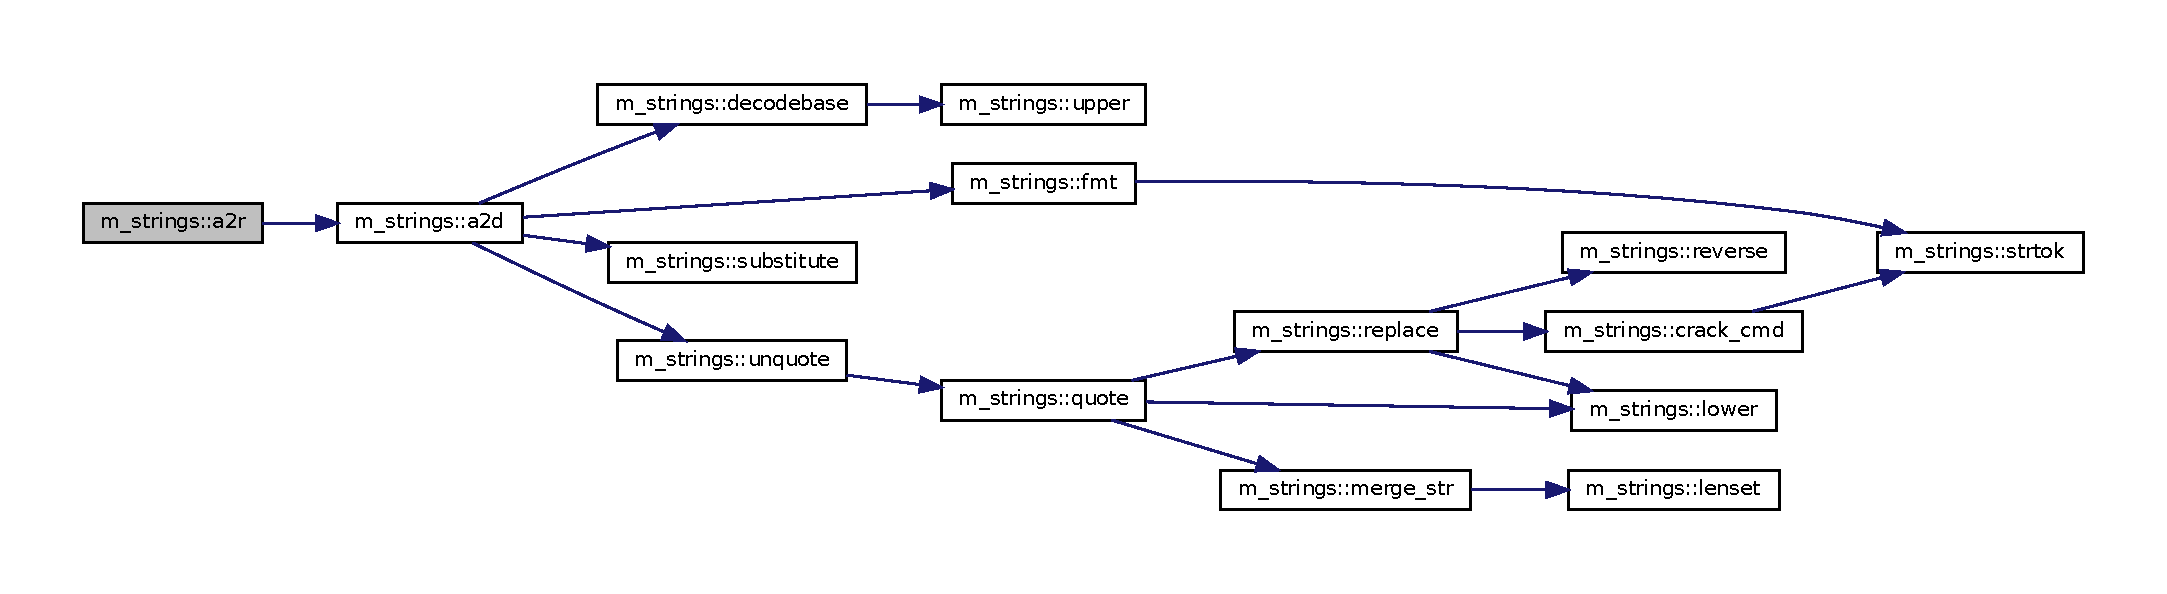
\includegraphics[width=350pt]{namespacem__strings_a6b4babf586dc3586426b13e4bb0fb979_cgraph}
\end{center}
\end{figure}
\mbox{\Hypertarget{namespacem__strings_a9365ae5277199446d93fc5208be2e9a5}\label{namespacem__strings_a9365ae5277199446d93fc5208be2e9a5}} 
\index{m\+\_\+strings@{m\+\_\+strings}!a2s@{a2s}}
\index{a2s@{a2s}!m\+\_\+strings@{m\+\_\+strings}}
\subsubsection{\texorpdfstring{a2s()}{a2s()}}
{\footnotesize\ttfamily pure character(len=size(array)) function, private m\+\_\+strings\+::a2s (\begin{DoxyParamCaption}\item[{character(len=1), dimension(\+:), intent(in)}]{array }\end{DoxyParamCaption})\hspace{0.3cm}{\ttfamily [private]}}



\subsubsection*{N\+A\+ME}

switch(3f) -\/ \mbox{[}M\+\_\+strings\+:A\+R\+R\+AY\mbox{]} converts between C\+H\+A\+R\+A\+C\+T\+ER scalar and array of single characters (L\+I\+C\+E\+N\+SE\+:PD)

\subsubsection*{S\+Y\+N\+O\+P\+S\+IS}

\begin{DoxyVerb}pure function switch(array) result (string)

 character(len=1),intent(in) :: array(:)
 character(len=SIZE(array))  :: string

  or

pure function switch(string) result (array)

 character(len=1),intent(in) :: array(:)
 character(len=SIZE(array))  :: string
\end{DoxyVerb}
 \subsubsection*{D\+E\+S\+C\+R\+I\+P\+T\+I\+ON}

\begin{DoxyVerb}SWITCH(3f): generic function that switches CHARACTER string to an array
of single characters or an array of single characters to a CHARACTER
string. Useful in passing strings to C. New Fortran features may
supersede these routines.
\end{DoxyVerb}


\subsubsection*{E\+X\+A\+M\+P\+L\+ES}

Sample program\+: \begin{DoxyVerb}program demo_switch
use M_strings, only : switch, isalpha, islower, nospace
character(len=*),parameter :: dashes='-----------------------------------'
character(len=*),parameter :: string='This is a string of letters'
character(len=1024)        :: line

! First, examples of standard Fortran features
write(*,*)['A','=','=','=','=','='].eq.'='      ! returns array [F,T,T,T,T,T]
write(*,*)all(['=','=','=','=','=','='].eq.'=') ! this would return T
write(*,*)all(['A','=','=','=','=','='].eq.'=') ! this would return F

! so to test if the string DASHES is all dashes using SWITCH(3f) is
if(all(switch(dashes).eq.'-'))then
   write(*,*)'DASHES is all dashes'
endif

! so to test is a string is all letters
! isalpha(3f) returns .true. only if character is a letter
write(*,*) all(isalpha(switch(dashes)))  ! false because dashes are not a letter
write(*,*) all(isalpha(switch(string)))  ! false because of spaces
write(*,*) all(isalpha(switch(nospace(string))))  ! true because removed whitespace

! to see if a string is all uppercase
write(*,*) string                           ! show the string
write(*,'(1x,*("[",a,"]":))') switch(string)   ! converted to character array
write(*,'(*(l3))') islower(switch(string))

line=nospace(string)                        ! we need a string that is all letters
write(*,*)'LINE=',trim(line)
write(*,*) islower(switch(nospace(string))) ! all true except first character
write(*,*) all(islower(switch(nospace(string))))      ! should be false
write(*,*) all(islower(switch(nospace(string(2:)))))  ! should be true

end program demo_switch
\end{DoxyVerb}


Expected output

$>$ F T T T T T $>$ T $>$ F $>$ D\+A\+S\+H\+ES is all dashes $>$ F $>$ F $>$ T $>$ This is a string of letters $>$ \mbox{[}T\mbox{]}\mbox{[}h\mbox{]}\mbox{[}i\mbox{]}\mbox{[}s\mbox{]}\mbox{[} \mbox{]}\mbox{[}i\mbox{]}\mbox{[}s\mbox{]}\mbox{[} \mbox{]}\mbox{[}a\mbox{]}\mbox{[} \mbox{]}\mbox{[}s\mbox{]}\mbox{[}t\mbox{]}\mbox{[}r\mbox{]}\mbox{[}i\mbox{]}\mbox{[}n\mbox{]}\mbox{[}g\mbox{]}\mbox{[} \mbox{]}\mbox{[}o\mbox{]}\mbox{[}f\mbox{]}\mbox{[} \mbox{]}\mbox{[}l\mbox{]}\mbox{[}e\mbox{]}\mbox{[}t\mbox{]}\mbox{[}t\mbox{]}\mbox{[}e\mbox{]}\mbox{[}r\mbox{]}\mbox{[}s\mbox{]} $>$ F T T T F T T F T F T T T T T T F T T F T T T T T T T $>$ L\+I\+NE=Thisisastringofletters $>$ F T T T T T T T T T T T T T T T T T T T T T $>$ F $>$ T \subsubsection*{A\+U\+T\+H\+OR}

John S. Urban \subsubsection*{L\+I\+C\+E\+N\+SE}

Public Domain \mbox{\Hypertarget{namespacem__strings_a1cacb2e45c7e3d7ed4cc1b183c35f323}\label{namespacem__strings_a1cacb2e45c7e3d7ed4cc1b183c35f323}} 
\index{m\+\_\+strings@{m\+\_\+strings}!adjustc@{adjustc}}
\index{adjustc@{adjustc}!m\+\_\+strings@{m\+\_\+strings}}
\subsubsection{\texorpdfstring{adjustc()}{adjustc()}}
{\footnotesize\ttfamily pure character(len=\+:) function, allocatable, public m\+\_\+strings\+::adjustc (\begin{DoxyParamCaption}\item[{character(len=$\ast$), intent(in)}]{string,  }\item[{integer, intent(in), optional}]{length }\end{DoxyParamCaption})}



\subsubsection*{N\+A\+ME}

adjustc(3f) -\/ \mbox{[}M\+\_\+strings\+:W\+H\+I\+T\+E\+S\+P\+A\+CE\mbox{]} center text (L\+I\+C\+E\+N\+SE\+:PD) 

\subsubsection*{S\+Y\+N\+O\+P\+S\+IS}

pure function adjustc(string\mbox{[},length\mbox{]})

character(len=$\ast$),intent(in) \+:\+: string integer,intent(in),optional \+:\+: length character(len=\+:),allocatable \+:\+: adjustc \subsubsection*{D\+E\+S\+C\+R\+I\+P\+T\+I\+ON}

Centers input text in a string of the length specified. Returns a string of length L\+E\+N\+G\+TH if L\+E\+N\+G\+TH is present. Otherwise returns a string of the length of the input string. \subsubsection*{O\+P\+T\+I\+O\+NS}

string input string to trim and center length line length to center text in, optional. \subsubsection*{R\+E\+T\+U\+R\+NS}

adjustc centered output string

\subsubsection*{E\+X\+A\+M\+P\+L\+ES}

Sample Program\+: \begin{DoxyVerb}program demo_adjustc
use M_strings, only : adjustc
!  using length of the input string
   write(*,'(a)')       '================================'
   write(*,'(a)')adjustc('centered string                 ')
   write(*,'(a)')adjustc('                 centered string')
   write(*,'(a)')adjustc('  centered string               ')
!  using explicit output string length
   write(*,'(a)')repeat('=',50)
   write(*,'(a)')adjustc('this is a centered string',50)
   write(*,'(a)')repeat('=',50)
end program demo_adjustc
\end{DoxyVerb}


Expected output 

 centered string centered string \subsection*{centered string }

\subsection*{this is a centered string }

\subsubsection*{A\+U\+T\+H\+OR}

John S. Urban \subsubsection*{L\+I\+C\+E\+N\+SE}

Public Domain


\begin{DoxyParams}[1]{Parameters}
\mbox{\tt in}  & {\em string} & P\+R\+O\+C\+E\+D\+U\+RE adjustc(3f) D\+E\+S\+C\+R\+I\+P\+T\+I\+ON center text using implicit or explicit length \subsubsection*{V\+E\+R\+S\+I\+ON 2.\+0, 20160711}\\
\hline
\end{DoxyParams}
A\+U\+T\+H\+OR John S. Urban \mbox{\Hypertarget{namespacem__strings_ab20ba3a07833232eb3c67d4020a7fe64}\label{namespacem__strings_ab20ba3a07833232eb3c67d4020a7fe64}} 
\index{m\+\_\+strings@{m\+\_\+strings}!atleast@{atleast}}
\index{atleast@{atleast}!m\+\_\+strings@{m\+\_\+strings}}
\subsubsection{\texorpdfstring{atleast()}{atleast()}}
{\footnotesize\ttfamily function, public m\+\_\+strings\+::atleast (\begin{DoxyParamCaption}\item[{character(len=$\ast$), intent(in)}]{line,  }\item[{integer, intent(in)}]{length,  }\item[{character(len=$\ast$), intent(in), optional}]{pattern }\end{DoxyParamCaption})}



\subsubsection*{N\+A\+ME}

atleast(3f) -\/ \mbox{[}M\+\_\+strings\+:L\+E\+N\+G\+TH\mbox{]} return string padded to at least specified length (L\+I\+C\+E\+N\+SE\+:PD) 

\subsubsection*{S\+Y\+N\+O\+P\+S\+IS}

function atleast(str,length,pattern) result(strout)

character(len=$\ast$) \+:\+: str integer,intent(in) \+:\+: length character(len=max(length,len(trim(line)))) \+:\+: strout character(len=$\ast$),optional \+:\+: pattern \subsubsection*{D\+E\+S\+C\+R\+I\+P\+T\+I\+ON}

atleast(3f) pads a string with spaces to at least the specified length. If the trimmed input string is longer than the requested length the trimmed string is returned. \subsubsection*{O\+P\+T\+I\+O\+NS}

str the input string to return trimmed, but then padded to the specified length if shorter than length length The minimum string length to return pattern optional string to use as padding. Defaults to a space. \subsubsection*{R\+E\+T\+U\+R\+NS}

strout The input string padded to the requested length or the trimmed input string if the input string is longer than the requested length.

\subsubsection*{E\+X\+A\+M\+P\+LE}

Sample Program\+: \begin{DoxyVerb}program demo_atleast
 use M_strings, only : atleast
 implicit none
 character(len=10)            :: string='abcdefghij'
 character(len=:),allocatable :: answer
 integer                      :: i
    answer=atleast(string,5)
    write(*,'("[",a,"]")') answer
    answer=atleast(string,20)
    write(*,'("[",a,"]")') answer
    i=30
    write(*,*)
    write(*,'(1x,a,i0)') atleast('CHAPTER 1 : The beginning ',i,'.'), 1
    write(*,'(1x,a,i0)') atleast('CHAPTER 2 : The end ',i,'.'),       1234
    write(*,'(1x,a,i0)') atleast('APPENDIX ',i,'.'),                  1235
    write(*,*)
    write(*,'(1x,a,i7)') atleast('CHAPTER 1 : The beginning ',i,'.'), 1
    write(*,'(1x,a,i7)') atleast('CHAPTER 2 : The end ',i,'.'),       1234
    write(*,'(1x,a,i7)') atleast('APPENDIX ',i,'.'),                  1235
end program demo_atleast
\end{DoxyVerb}


Results\+: \begin{DoxyVerb}[abcdefghij]
[abcdefghij          ]

 CHAPTER 1 : The beginning ....1
 CHAPTER 2 : The end ..........1234
 APPENDIX .....................1235

 CHAPTER 1 : The beginning ....      1
 CHAPTER 2 : The end ..........   1234
 APPENDIX .....................   1235
\end{DoxyVerb}
 \subsubsection*{A\+U\+T\+H\+OR}

John S. Urban \subsubsection*{L\+I\+C\+E\+N\+SE}

Public Domain Here is the caller graph for this function\+:\nopagebreak
\begin{figure}[H]
\begin{center}
\leavevmode
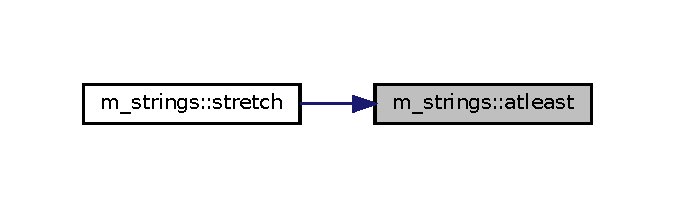
\includegraphics[width=324pt]{namespacem__strings_ab20ba3a07833232eb3c67d4020a7fe64_icgraph}
\end{center}
\end{figure}
\mbox{\Hypertarget{namespacem__strings_a635ef6f1dd73400e7b339392886d6357}\label{namespacem__strings_a635ef6f1dd73400e7b339392886d6357}} 
\index{m\+\_\+strings@{m\+\_\+strings}!base@{base}}
\index{base@{base}!m\+\_\+strings@{m\+\_\+strings}}
\subsubsection{\texorpdfstring{base()}{base()}}
{\footnotesize\ttfamily logical function, public m\+\_\+strings\+::base (\begin{DoxyParamCaption}\item[{character(len=$\ast$), intent(in)}]{x,  }\item[{integer, intent(in)}]{b,  }\item[{character(len=$\ast$), intent(out)}]{y,  }\item[{integer, intent(in)}]{a }\end{DoxyParamCaption})}



\subsubsection*{N\+A\+ME}

base(3f) -\/ \mbox{[}M\+\_\+strings\+:B\+A\+SE\mbox{]} convert whole number string in base \mbox{[}2-\/36\mbox{]} to string in alternate base \mbox{[}2-\/36\mbox{]} (L\+I\+C\+E\+N\+SE\+:PD) 

\subsubsection*{S\+Y\+N\+O\+P\+S\+IS}

logical function base(x,b,y,a)

character(len=$\ast$),intent(in) \+:\+: x character(len=$\ast$),intent(out) \+:\+: y integer,intent(in) \+:\+: b,a \subsubsection*{D\+E\+S\+C\+R\+I\+P\+T\+I\+ON}

\begin{DoxyVerb}Convert a numeric string from base B to base A. The function returns
FALSE if B is not in the range [2..36] or if string X contains invalid
characters in base B or if result Y is too big

The letters A,B,...,Z represent 10,11,...,36 in the base > 10.
\end{DoxyVerb}


\subsubsection*{O\+P\+T\+I\+O\+NS}

x input string representing numeric whole value b assumed base of input string y output string a base specified for output string

\subsubsection*{E\+X\+A\+M\+P\+LE}

Sample program\+: \begin{DoxyVerb}program demo_base
use M_strings, only : base
implicit none
integer           :: ba,bd
character(len=40) :: x,y

print *,' BASE CONVERSION'
write(*,'("Start   Base (2 to 36): ")',advance='no'); read *, bd
write(*,'("Arrival Base (2 to 36): ")',advance='no'); read *, ba
INFINITE: do
   write(*,'("Enter number in start base: ")',advance='no'); read *, x
   if(x.eq.'0') exit INFINITE
   if(base(x,bd,y,ba))then
        write(*,'("In base ",I2,": ",A20)')  ba, y
    else
      print *,'Error in decoding/encoding number.'
    endif
 enddo INFINITE

 end program demo_base
\end{DoxyVerb}


\subsubsection*{A\+U\+T\+H\+OR}

John S. Urban \subsubsection*{L\+I\+C\+E\+N\+SE}

Public Domain 

References codebase(), and decodebase().

Here is the call graph for this function\+:\nopagebreak
\begin{figure}[H]
\begin{center}
\leavevmode
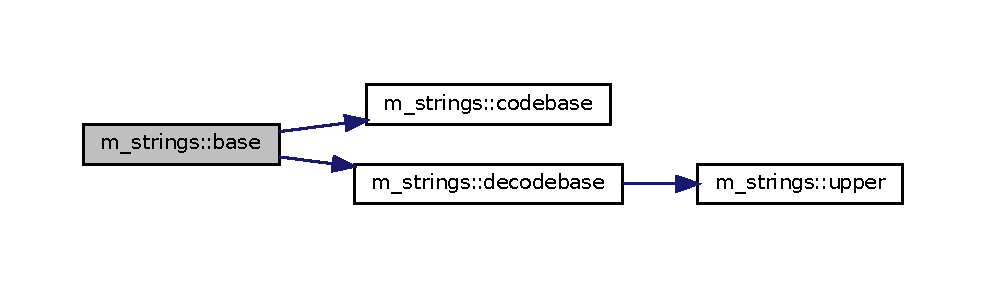
\includegraphics[width=350pt]{namespacem__strings_a635ef6f1dd73400e7b339392886d6357_cgraph}
\end{center}
\end{figure}
Here is the caller graph for this function\+:\nopagebreak
\begin{figure}[H]
\begin{center}
\leavevmode
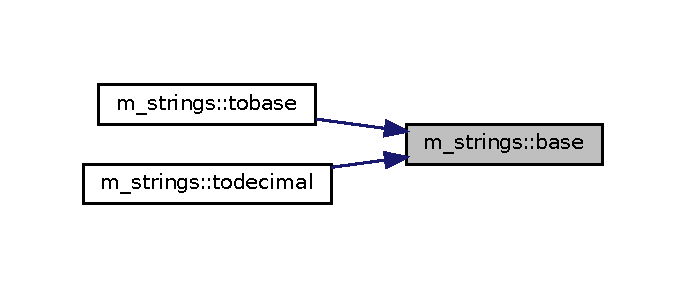
\includegraphics[width=329pt]{namespacem__strings_a635ef6f1dd73400e7b339392886d6357_icgraph}
\end{center}
\end{figure}
\mbox{\Hypertarget{namespacem__strings_a0a8c0c16a34208351523068686cb743b}\label{namespacem__strings_a0a8c0c16a34208351523068686cb743b}} 
\index{m\+\_\+strings@{m\+\_\+strings}!c2s@{c2s}}
\index{c2s@{c2s}!m\+\_\+strings@{m\+\_\+strings}}
\subsubsection{\texorpdfstring{c2s()}{c2s()}}
{\footnotesize\ttfamily character(len=\+:) function, allocatable, public m\+\_\+strings\+::c2s (\begin{DoxyParamCaption}\item[{type(c\+\_\+ptr), intent(in)}]{c\+\_\+string\+\_\+pointer }\end{DoxyParamCaption})}



\subsubsection*{N\+A\+ME}

c2s(3f) -\/ \mbox{[}M\+\_\+strings\+:A\+R\+R\+AY\mbox{]} convert C string pointer to Fortran character string (L\+I\+C\+E\+N\+SE\+:PD) 

\subsubsection*{S\+Y\+N\+O\+P\+S\+IS}

\begin{DoxyVerb}function c2s(c_string_pointer) result(f_string)

 type(c_ptr), intent(in)       :: c_string_pointer
 character(len=:), allocatable :: f_string
\end{DoxyVerb}
 \subsubsection*{D\+E\+S\+C\+R\+I\+P\+T\+I\+ON}

Given a C pointer to a character string return a Fortran character string. \subsubsection*{O\+P\+T\+I\+O\+NS}

c\+\_\+string\+\_\+pointer C pointer to convert \subsubsection*{R\+E\+T\+U\+R\+NS}

f\+\_\+string Fortran character variable to return \subsubsection*{E\+X\+A\+M\+P\+LE}

\subsubsection*{A\+U\+T\+H\+OR}

John S. Urban \subsubsection*{L\+I\+C\+E\+N\+SE}

Public Domain \mbox{\Hypertarget{namespacem__strings_a1222f3b718f7637105bde330367925e1}\label{namespacem__strings_a1222f3b718f7637105bde330367925e1}} 
\index{m\+\_\+strings@{m\+\_\+strings}!change@{change}}
\index{change@{change}!m\+\_\+strings@{m\+\_\+strings}}
\subsubsection{\texorpdfstring{change()}{change()}}
{\footnotesize\ttfamily subroutine, public m\+\_\+strings\+::change (\begin{DoxyParamCaption}\item[{character(len=$\ast$), intent(inout)}]{target\+\_\+string,  }\item[{character(len=$\ast$), intent(in)}]{cmd,  }\item[{integer}]{ierr }\end{DoxyParamCaption})}



\subsubsection*{N\+A\+ME}

change(3f) -\/ \mbox{[}M\+\_\+strings\+:E\+D\+I\+T\+I\+NG\mbox{]} change old string to new string with a directive like a line editor (L\+I\+C\+E\+N\+SE\+:PD) 

\subsubsection*{S\+Y\+N\+O\+P\+S\+IS}

\begin{DoxyVerb}subroutine change(target_string,cmd,ierr)

 character(len=*),intent(inout) :: target_string
 character(len=*),intent(in)    :: cmd
 integer                        :: ierr
\end{DoxyVerb}
 \subsubsection*{D\+E\+S\+C\+R\+I\+P\+T\+I\+ON}

change an old substring into a new substring in a character variable like a line editor. Primarily used to create interactive utilities such as input history editors for interactive line-\/mode programs. The output string is assumed long enough to accommodate the change. a directive resembles a line editor directive of the form

C/old\+\_\+string/new\+\_\+string/

where / may be any character which is not included in old\+\_\+string or new\+\_\+string.

a null old\+\_\+string implies \char`\"{}beginning of string\char`\"{}.

\subsubsection*{O\+P\+T\+I\+O\+NS}

target\+\_\+string line to be changed cmd contains instructions to change the string ierr error code.

o =-\/1 bad directive o =0 no changes made o $>$0 count of changes made

\subsubsection*{E\+X\+A\+M\+P\+L\+ES}

Sample program\+:

program demo\+\_\+change \begin{DoxyVerb}use M_strings, only : change
implicit none
character(len=132) :: line='This is a test string to change'
integer            :: ierr
   write(*,*)trim(line)
   ! change miniscule a to uppercase A
   call change(line,'c/a/A/',ierr)
   write(*,*)trim(line)
   ! put string at beginning of line
   call change(line,'c//prefix: /',ierr)
   write(*,*)trim(line)
   ! remove blanks
   call change(line,'c/ //',ierr)
   write(*,*)trim(line)
\end{DoxyVerb}
 end program demo\+\_\+change

Expected output \begin{DoxyVerb} This is a test string to change
 This is A test string to chAnge
 prefix: This is A test string to chAnge
 prefix:ThisisAteststringtochAnge
\end{DoxyVerb}
 \subsubsection*{A\+U\+T\+H\+OR}

John S. Urban \subsubsection*{L\+I\+C\+E\+N\+SE}

Public Domain 

References strtok(), and substitute().

Here is the call graph for this function\+:\nopagebreak
\begin{figure}[H]
\begin{center}
\leavevmode
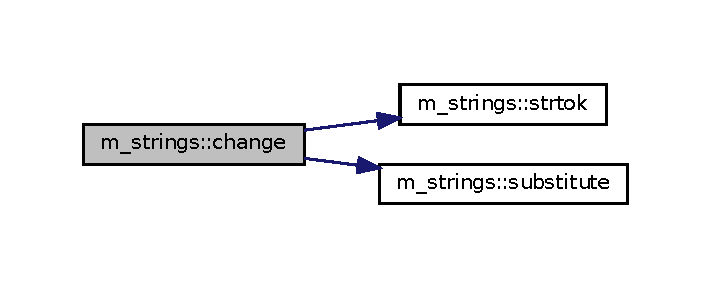
\includegraphics[width=341pt]{namespacem__strings_a1222f3b718f7637105bde330367925e1_cgraph}
\end{center}
\end{figure}
\mbox{\Hypertarget{namespacem__strings_aa3fc15a665eeff512b7f5269029f558d}\label{namespacem__strings_aa3fc15a665eeff512b7f5269029f558d}} 
\index{m\+\_\+strings@{m\+\_\+strings}!chomp@{chomp}}
\index{chomp@{chomp}!m\+\_\+strings@{m\+\_\+strings}}
\subsubsection{\texorpdfstring{chomp()}{chomp()}}
{\footnotesize\ttfamily integer function, public m\+\_\+strings\+::chomp (\begin{DoxyParamCaption}\item[{character(len=$\ast$)}]{source\+\_\+string,  }\item[{character(len=\+:), intent(out), allocatable}]{token,  }\item[{character(len=$\ast$), intent(in), optional}]{delimiters }\end{DoxyParamCaption})}



\subsubsection*{N\+A\+ME}

chomp(3f) -\/ \mbox{[}M\+\_\+strings\+:T\+O\+K\+E\+NS\mbox{]} Tokenize a string, consuming it one token per call (L\+I\+C\+E\+N\+SE\+:PD) 

\subsubsection*{S\+Y\+N\+O\+P\+S\+IS}

\begin{DoxyVerb}function chomp(source_string,token[,delimiters])

 character(len=*)                     :: source_string
 character(len=:),intent(out),token   :: token
 character(len=:),intent(in),optional :: delimiters
 integer                              :: chomp
\end{DoxyVerb}
 \subsubsection*{D\+E\+S\+C\+R\+I\+P\+T\+I\+ON}

The C\+H\+O\+M\+P(3f) function is used to isolate sequential tokens in a string, S\+O\+U\+R\+C\+E\+\_\+\+S\+T\+R\+I\+NG. These tokens are delimited in the string by at least one of the characters in D\+E\+L\+I\+M\+I\+T\+E\+RS. This routine consumes the source\+\_\+string one token per call. It returns -\/1 when complete. The default delimiter list is \char`\"{}space,tab,carriage return,newline\char`\"{}.

\subsubsection*{O\+P\+T\+I\+O\+NS}

S\+O\+U\+R\+C\+E\+\_\+\+S\+T\+R\+I\+NG string to tokenize D\+E\+L\+I\+M\+I\+T\+E\+RS list of separator characters

\subsubsection*{R\+E\+T\+U\+R\+NS}

T\+O\+K\+EN returned token C\+H\+O\+MP status flag. 0 = success, -\/1 = no tokens remain

\subsubsection*{E\+X\+A\+M\+P\+L\+ES}

Sample program\+: \begin{DoxyVerb} program demo_chomp

 use M_strings, only : chomp
 implicit none
 character(len=100)            :: inline
 character(len=:),allocatable  :: token
 character(len=*),parameter    :: delimiters=' ;,'
 integer                       :: ios
 integer                       :: icount
 integer                       :: itoken
    icount=0
    do        ! read lines from stdin until end-of-file or error
       read (unit=*,fmt="(a)",iostat=ios) inline
       if(ios.ne.0)stop
       icount=icount+1
       itoken=0
       write(*,*)'INLINE ',trim(inline)
       do while ( chomp(inline,token,delimiters).ge. 0)
          itoken=itoken+1
          print *, itoken,'TOKEN=['//trim(token)//']'
       enddo
    enddo

 end program demo_chomp
\end{DoxyVerb}


sample input file \begin{DoxyVerb} this is a test of chomp; A:B :;,C;;
\end{DoxyVerb}


sample output file

I\+N\+L\+I\+NE this is a test of chomp; A\+:B \+:;,C;; 1 T\+O\+K\+EN=\mbox{[}this\mbox{]} 2 T\+O\+K\+EN=\mbox{[}is\mbox{]} 3 T\+O\+K\+EN=\mbox{[}a\mbox{]} 4 T\+O\+K\+EN=\mbox{[}test\mbox{]} 5 T\+O\+K\+EN=\mbox{[}of\mbox{]} 6 T\+O\+K\+EN=\mbox{[}chomp\mbox{]} 7 T\+O\+K\+EN=\mbox{[}A\+:B\mbox{]} 8 T\+O\+K\+EN=\mbox{[}\+:\mbox{]} 9 T\+O\+K\+EN=\mbox{[}C\mbox{]}

\subsubsection*{A\+U\+T\+H\+OR}

John S. Urban \subsubsection*{L\+I\+C\+E\+N\+SE}

Public Domain \mbox{\Hypertarget{namespacem__strings_a3a022b64dc902dc6043e3f265ee78e38}\label{namespacem__strings_a3a022b64dc902dc6043e3f265ee78e38}} 
\index{m\+\_\+strings@{m\+\_\+strings}!codebase@{codebase}}
\index{codebase@{codebase}!m\+\_\+strings@{m\+\_\+strings}}
\subsubsection{\texorpdfstring{codebase()}{codebase()}}
{\footnotesize\ttfamily logical function, public m\+\_\+strings\+::codebase (\begin{DoxyParamCaption}\item[{integer, intent(in)}]{inval10,  }\item[{integer, intent(in)}]{outbase,  }\item[{character(len=$\ast$), intent(out)}]{answer }\end{DoxyParamCaption})}



\subsubsection*{N\+A\+ME}

codebase(3f) -\/ \mbox{[}M\+\_\+strings\+:B\+A\+SE\mbox{]} convert whole number in base 10 to string in base \mbox{[}2-\/36\mbox{]} (L\+I\+C\+E\+N\+SE\+:PD)

\subsubsection*{S\+Y\+N\+O\+P\+S\+IS}

logical function codebase(in\+\_\+base10,out\+\_\+base,answer)

integer,intent(in) \+:\+: in\+\_\+base10 integer,intent(in) \+:\+: out\+\_\+base character(len=$\ast$),intent(out) \+:\+: answer \subsubsection*{D\+E\+S\+C\+R\+I\+P\+T\+I\+ON}

\begin{DoxyVerb}Convert a number from base 10 to base OUT_BASE. The function returns
.FALSE. if OUT_BASE is not in [2..36] or if number IN_BASE10 is
too big.

The letters A,B,...,Z represent 10,11,...,36 in the base > 10.
\end{DoxyVerb}


\subsubsection*{E\+X\+A\+M\+P\+LE}

Sample program\+: \begin{DoxyVerb}program demo_codebase
use M_strings, only : codebase
implicit none
character(len=20) :: answer
integer           :: i, j
logical           :: ierr
do j=1,100
   do i=2,36
      ierr=codebase(j,i,answer)
      write(*,*)'VALUE=',j,' BASE=',i,' ANSWER=',answer
   enddo
enddo
end program demo_codebase
\end{DoxyVerb}


\subsubsection*{A\+U\+T\+H\+OR}

John S. Urban

Ref.\+: "Math matiques en Turbo-\/\+Pascal by M. Ducamp and A. Reverchon (2), Eyrolles, Paris, 1988".

based on a F90 Version By J-\/P Moreau (www.\+jpmoreau.\+fr)

\subsubsection*{L\+I\+C\+E\+N\+SE}

Public Domain Here is the caller graph for this function\+:\nopagebreak
\begin{figure}[H]
\begin{center}
\leavevmode
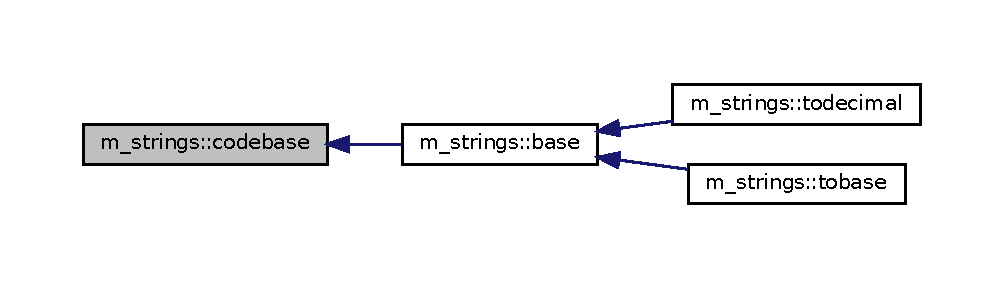
\includegraphics[width=350pt]{namespacem__strings_a3a022b64dc902dc6043e3f265ee78e38_icgraph}
\end{center}
\end{figure}
\mbox{\Hypertarget{namespacem__strings_a929c032267cb990ad4991fab4aed1d57}\label{namespacem__strings_a929c032267cb990ad4991fab4aed1d57}} 
\index{m\+\_\+strings@{m\+\_\+strings}!compact@{compact}}
\index{compact@{compact}!m\+\_\+strings@{m\+\_\+strings}}
\subsubsection{\texorpdfstring{compact()}{compact()}}
{\footnotesize\ttfamily character(len=len(str)) function, public m\+\_\+strings\+::compact (\begin{DoxyParamCaption}\item[{character(len=$\ast$), intent(in)}]{str,  }\item[{character(len=$\ast$), intent(in), optional}]{char }\end{DoxyParamCaption})}



\subsubsection*{N\+A\+ME}

compact(3f) -\/ \mbox{[}M\+\_\+strings\+:W\+H\+I\+T\+E\+S\+P\+A\+CE\mbox{]} converts contiguous whitespace to a single character (or nothing) (L\+I\+C\+E\+N\+SE\+:PD) 

\subsubsection*{S\+Y\+N\+O\+P\+S\+IS}

\begin{DoxyVerb}function compact(STR,CHAR) result (OUTSTR)

 character(len=*),intent(in)          :: STR
 character(len=*),intent(in),optional :: CHAR
 character(len=len(str))              :: OUTSTR
\end{DoxyVerb}
 \subsubsection*{D\+E\+S\+C\+R\+I\+P\+T\+I\+ON}

C\+O\+M\+P\+A\+C\+T(3f) converts multiple spaces, tabs and control characters (called \char`\"{}whitespace\char`\"{}) to a single character or nothing. Leading whitespace is removed.

\subsubsection*{O\+P\+T\+I\+O\+NS}

S\+TR input string to reduce or remove whitespace from C\+H\+AR By default the character that replaces adjacent whitespace is a space. If the optional C\+H\+AR parameter is supplied it will be used to replace the whitespace. If a null character is supplied for C\+H\+AR whitespace is removed. \subsubsection*{R\+E\+T\+U\+R\+NS}

O\+U\+T\+S\+TR string of same length as input string but with all contiguous whitespace reduced to a single space and leading whitespace removed

\subsubsection*{E\+X\+A\+M\+P\+L\+ES}

Sample Program\+: \begin{DoxyVerb}program demo_compact
 use M_strings, only : compact
 implicit none
 ! produces 'This is a test               '
 write(*,*)compact('  This     is      a     test  ')
 ! produces 'Thisisatest                  '
 write(*,*)compact('  This     is      a     test  ',char='')
 ! produces 'This:is:a:test               '
 write(*,*)compact('  This     is      a     test  ',char=':')
 ! note CHAR is used to replace the whitespace, but if CHAR is
 ! in the original string it is just copied
 write(*,*)compact('A  AA    A   AAAAA',char='A')
 ! produces (original A characters are left as-is) 'AAAAAAAAAAAA'
 ! not 'A'
end program demo_compact
\end{DoxyVerb}


Expected output

$>$This is a test $>$Thisisatest $>$This\+:is\+:a\+:test $>$A\+A\+A\+A\+A\+A\+A\+A\+A\+A\+AA \subsubsection*{A\+U\+T\+H\+OR}

John S. Urban \subsubsection*{L\+I\+C\+E\+N\+SE}

Public Domain 

References nospace().

Here is the call graph for this function\+:\nopagebreak
\begin{figure}[H]
\begin{center}
\leavevmode
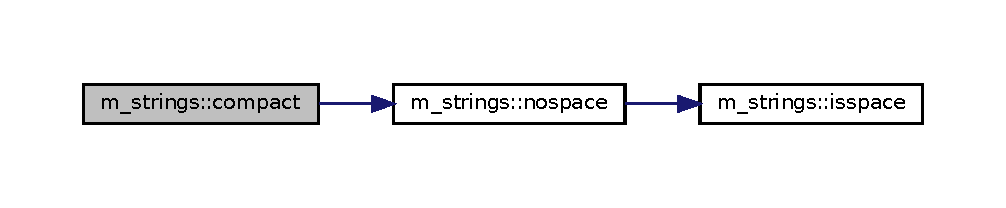
\includegraphics[width=350pt]{namespacem__strings_a929c032267cb990ad4991fab4aed1d57_cgraph}
\end{center}
\end{figure}
\mbox{\Hypertarget{namespacem__strings_a818d715927dd61c1be6df5d2cdec4e4c}\label{namespacem__strings_a818d715927dd61c1be6df5d2cdec4e4c}} 
\index{m\+\_\+strings@{m\+\_\+strings}!crack\+\_\+cmd@{crack\+\_\+cmd}}
\index{crack\+\_\+cmd@{crack\+\_\+cmd}!m\+\_\+strings@{m\+\_\+strings}}
\subsubsection{\texorpdfstring{crack\+\_\+cmd()}{crack\_cmd()}}
{\footnotesize\ttfamily subroutine m\+\_\+strings\+::crack\+\_\+cmd (\begin{DoxyParamCaption}\item[{character(len=$\ast$), intent(in)}]{cmd,  }\item[{character(len=\+:), intent(out), allocatable}]{old,  }\item[{character(len=\+:), intent(out), allocatable}]{new,  }\item[{integer}]{ierr }\end{DoxyParamCaption})\hspace{0.3cm}{\ttfamily [private]}}



\subsubsection*{N\+A\+ME}

replace(3f) -\/ \mbox{[}M\+\_\+strings\+:E\+D\+I\+T\+I\+NG\mbox{]} function globally replaces one substring for another in string (L\+I\+C\+E\+N\+SE\+:PD) 

\subsubsection*{S\+Y\+N\+O\+P\+S\+IS}

\begin{DoxyVerb}function replace(targetline[,old,new|cmd],range,ierr) result (newline)

 character(len=*)                       :: targetline
 character(len=*),intent(in),optional   :: old
 character(len=*),intent(in),optional   :: new
 character(len=*),intent(in),optional   :: cmd
 integer,intent(in),optional            :: range(2)
 integer,intent(out),optional           :: ierr
 logical,intent(in),optional            :: clip
 character(len=:),allocatable           :: newline
\end{DoxyVerb}
 \subsubsection*{D\+E\+S\+C\+R\+I\+P\+T\+I\+ON}

Globally replace one substring for another in string. Either C\+MD or O\+LD and N\+EW must be specified.

\subsubsection*{O\+P\+T\+I\+O\+NS}

targetline input line to be changed old old substring to replace new new substring cmd alternate way to specify old and new string, in the form c/old/new/; where \char`\"{}/\char`\"{} can be any character not in \char`\"{}old\char`\"{} or \char`\"{}new\char`\"{} range if present, only change range(1) to range(2) of occurrences of old string ierr error code. iF ier = -\/1 bad directive, $>$= 0 then count of changes made clip whether to return trailing spaces or not. Defaults to .false. \subsubsection*{R\+E\+T\+U\+R\+NS}

newline allocatable string returned

\subsubsection*{E\+X\+A\+M\+P\+L\+ES}

Sample Program\+: \begin{DoxyVerb}program demo_replace
use M_strings, only : replace
implicit none
character(len=:),allocatable :: targetline

targetline='this is the input string'

call testit('th','TH','THis is THe input string')

! a null old substring means "at beginning of line"
call testit('','BEFORE:', 'BEFORE:THis is THe input string')

! a null new string deletes occurrences of the old substring
call testit('i','', 'BEFORE:THs s THe nput strng')

write(*,*)'Examples of the use of RANGE='

targetline=replace('a b ab baaa aaaa','a','A')
write(*,*)'replace a with A ['//targetline//']'

targetline=replace('a b ab baaa aaaa','a','A',range=[3,5])
write(*,*)'replace a with A instances 3 to 5 ['//targetline//']'

targetline=replace('a b ab baaa aaaa','a','',range=[3,5])
write(*,*)'replace a with null instances 3 to 5 ['//targetline//']'

targetline=replace('a b ab baaa aaaa aa aa a a a aa aaaaaa','aa','CCCC',range=[3,5])
write(*,*)'replace aa with CCCC instances 3 to 5 ['//targetline//']'

contains
subroutine testit(old,new,expected)
character(len=*),intent(in) :: old,new,expected
write(*,*)repeat('=',79)
write(*,*)'STARTED ['//targetline//']'
write(*,*)'OLD['//old//']', ' NEW['//new//']'
targetline=replace(targetline,old,new)
write(*,*)'GOT     ['//targetline//']'
write(*,*)'EXPECTED['//expected//']'
write(*,*)'TEST    [',targetline.eq.expected,']'
end subroutine testit

end program demo_replace
\end{DoxyVerb}


Expected output 

 S\+T\+A\+R\+T\+ED \mbox{[}this is the input string\mbox{]} O\+LD\mbox{[}th\mbox{]} N\+EW\mbox{[}TH\mbox{]} G\+OT \mbox{[}T\+His is T\+He input string\mbox{]} E\+X\+P\+E\+C\+T\+ED\mbox{[}T\+His is T\+He input string\mbox{]} \subsection*{T\+E\+ST \mbox{[} T \mbox{]} }

S\+T\+A\+R\+T\+ED \mbox{[}T\+His is T\+He input string\mbox{]} O\+LD\mbox{[}\mbox{]} N\+EW\mbox{[}B\+E\+F\+O\+RE\+:\mbox{]} G\+OT \mbox{[}B\+E\+F\+O\+RE\+:T\+His is T\+He input string\mbox{]} E\+X\+P\+E\+C\+T\+ED\mbox{[}B\+E\+F\+O\+RE\+:T\+His is T\+He input string\mbox{]} \subsection*{T\+E\+ST \mbox{[} T \mbox{]} }

S\+T\+A\+R\+T\+ED \mbox{[}B\+E\+F\+O\+RE\+:T\+His is T\+He input string\mbox{]} O\+LD\mbox{[}i\mbox{]} N\+EW\mbox{[}\mbox{]} G\+OT \mbox{[}B\+E\+F\+O\+RE\+:T\+Hs s T\+He nput strng\mbox{]} E\+X\+P\+E\+C\+T\+ED\mbox{[}B\+E\+F\+O\+RE\+:T\+Hs s T\+He nput strng\mbox{]} T\+E\+ST \mbox{[} T \mbox{]} Examples of the use of R\+A\+N\+GE= replace a with A \mbox{[}A b Ab b\+A\+AA A\+A\+AA\mbox{]} replace a with A instances 3 to 5 \mbox{[}a b ab b\+A\+AA aaaa\mbox{]} replace a with null instances 3 to 5 \mbox{[}a b ab b aaaa\mbox{]} replace aa with C\+C\+CC instances 3 to 5 \mbox{[}a b ab baaa aa\+C\+C\+CC C\+C\+CC C\+C\+CC a a a aa aaaaaa\mbox{]}

\subsubsection*{A\+U\+T\+H\+OR}

John S. Urban \subsubsection*{L\+I\+C\+E\+N\+SE}

Public Domain 

References strtok().

Here is the call graph for this function\+:\nopagebreak
\begin{figure}[H]
\begin{center}
\leavevmode
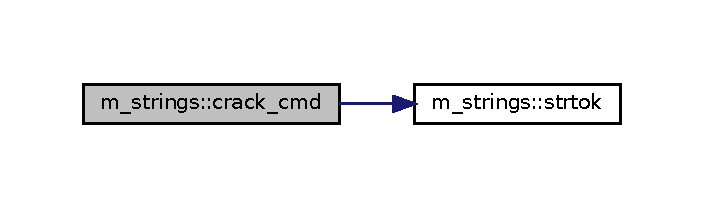
\includegraphics[width=338pt]{namespacem__strings_a818d715927dd61c1be6df5d2cdec4e4c_cgraph}
\end{center}
\end{figure}
Here is the caller graph for this function\+:\nopagebreak
\begin{figure}[H]
\begin{center}
\leavevmode
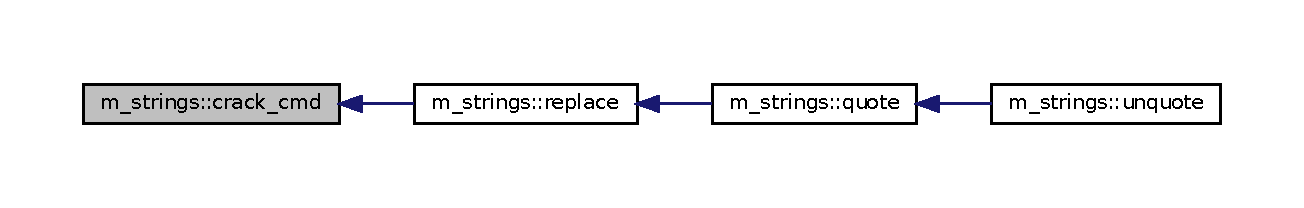
\includegraphics[width=350pt]{namespacem__strings_a818d715927dd61c1be6df5d2cdec4e4c_icgraph}
\end{center}
\end{figure}
\mbox{\Hypertarget{namespacem__strings_a7030d33ae9e65d8cf2e2cb9332ffdac0}\label{namespacem__strings_a7030d33ae9e65d8cf2e2cb9332ffdac0}} 
\index{m\+\_\+strings@{m\+\_\+strings}!crop@{crop}}
\index{crop@{crop}!m\+\_\+strings@{m\+\_\+strings}}
\subsubsection{\texorpdfstring{crop()}{crop()}}
{\footnotesize\ttfamily character(len=\+:) function, allocatable, public m\+\_\+strings\+::crop (\begin{DoxyParamCaption}\item[{character(len=$\ast$), intent(in)}]{strin }\end{DoxyParamCaption})}



\subsubsection*{N\+A\+ME}

crop(3f) -\/ \mbox{[}M\+\_\+strings\+:W\+H\+I\+T\+E\+S\+P\+A\+CE\mbox{]} trim leading blanks and trailing blanks from a string (L\+I\+C\+E\+N\+SE\+:PD) 

\subsubsection*{S\+Y\+N\+O\+P\+S\+IS}

\begin{DoxyVerb}function crop(strin) result (strout)

 character(len=*),intent(in)  :: strin
 character(len=:),allocatable :: strout
\end{DoxyVerb}
 \subsubsection*{D\+E\+S\+C\+R\+I\+P\+T\+I\+ON}

trim leading blanks from a string and return position of last non-\/blank character in the string. \subsubsection*{O\+P\+T\+I\+O\+NS}

strin input string to trim leading and trailing space from \subsubsection*{R\+E\+T\+U\+R\+NS}

strout cropped version of input string \subsubsection*{E\+X\+A\+M\+P\+LE}

Sample program\+: \begin{DoxyVerb}program demo_crop
use M_strings, only: crop
implicit none
character(len=20) ::  untrimmed = '   ABCDEFG abcdefg  '
   write(*,*) 'untrimmed string=[',untrimmed,']'
   write(*,*) 'cropped string=[',crop(untrimmed),']'
end program demo_crop
\end{DoxyVerb}


Expected output \begin{DoxyVerb}untrimmed string=[   ABCDEFG abcdefg                      ]
cropped string=[ABCDEFG abcdefg]
\end{DoxyVerb}
 \subsubsection*{A\+U\+T\+H\+OR}

John S. Urban \subsubsection*{L\+I\+C\+E\+N\+SE}

Public Domain \mbox{\Hypertarget{namespacem__strings_a14715e071aea9030b4c68c22fa5a455d}\label{namespacem__strings_a14715e071aea9030b4c68c22fa5a455d}} 
\index{m\+\_\+strings@{m\+\_\+strings}!d2s@{d2s}}
\index{d2s@{d2s}!m\+\_\+strings@{m\+\_\+strings}}
\subsubsection{\texorpdfstring{d2s()}{d2s()}}
{\footnotesize\ttfamily character(len=\+:) function, allocatable, private m\+\_\+strings\+::d2s (\begin{DoxyParamCaption}\item[{doubleprecision, intent(in)}]{dvalue,  }\item[{character(len=$\ast$), intent(in), optional}]{fmt }\end{DoxyParamCaption})\hspace{0.3cm}{\ttfamily [private]}}



References fmt(), and value\+\_\+to\+\_\+string().

Here is the call graph for this function\+:\nopagebreak
\begin{figure}[H]
\begin{center}
\leavevmode
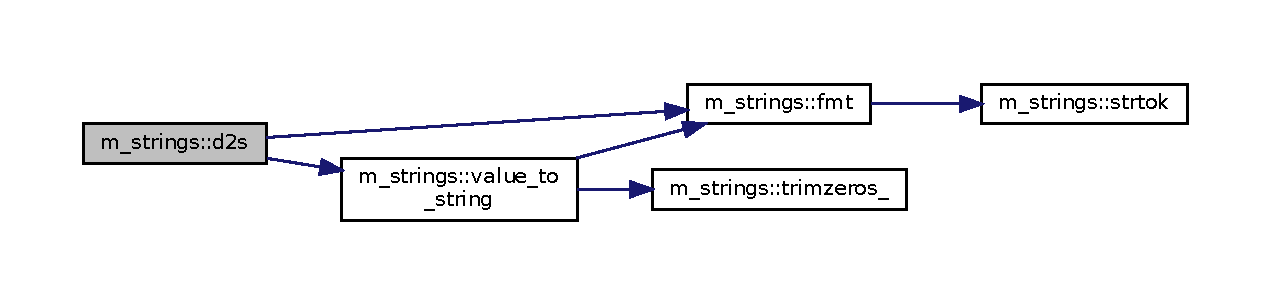
\includegraphics[width=350pt]{namespacem__strings_a14715e071aea9030b4c68c22fa5a455d_cgraph}
\end{center}
\end{figure}
\mbox{\Hypertarget{namespacem__strings_a970d99e3a2ab426bb90d6ea90bcc588a}\label{namespacem__strings_a970d99e3a2ab426bb90d6ea90bcc588a}} 
\index{m\+\_\+strings@{m\+\_\+strings}!dble\+\_\+s2v@{dble\+\_\+s2v}}
\index{dble\+\_\+s2v@{dble\+\_\+s2v}!m\+\_\+strings@{m\+\_\+strings}}
\subsubsection{\texorpdfstring{dble\+\_\+s2v()}{dble\_s2v()}}
{\footnotesize\ttfamily doubleprecision function m\+\_\+strings\+::dble\+\_\+s2v (\begin{DoxyParamCaption}\item[{character(len=$\ast$), intent(in)}]{chars }\end{DoxyParamCaption})\hspace{0.3cm}{\ttfamily [private]}}



References s2v().

Here is the call graph for this function\+:\nopagebreak
\begin{figure}[H]
\begin{center}
\leavevmode
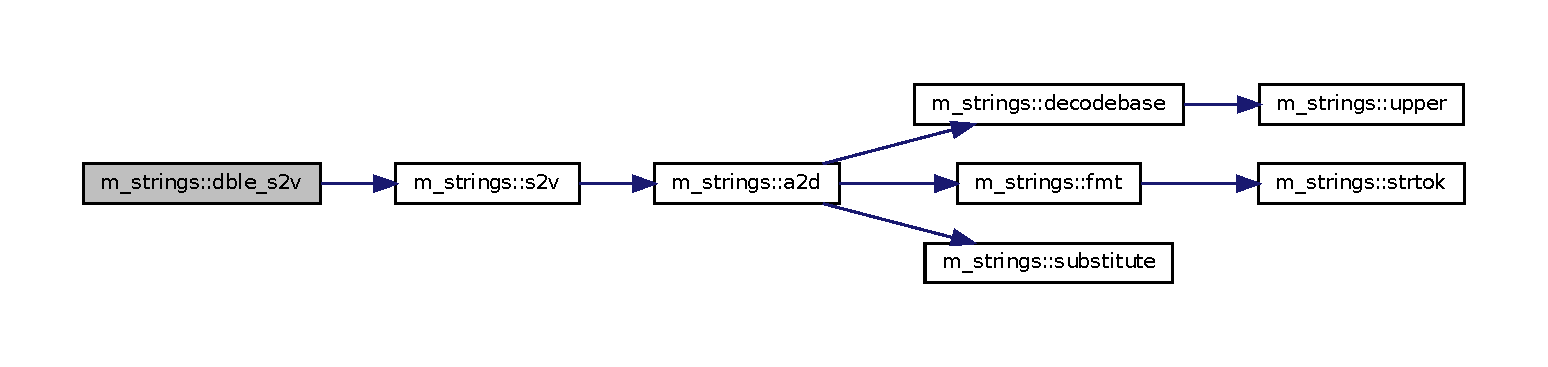
\includegraphics[width=350pt]{namespacem__strings_a970d99e3a2ab426bb90d6ea90bcc588a_cgraph}
\end{center}
\end{figure}
\mbox{\Hypertarget{namespacem__strings_ab463f9b431dd817b7b509608ec823b0f}\label{namespacem__strings_ab463f9b431dd817b7b509608ec823b0f}} 
\index{m\+\_\+strings@{m\+\_\+strings}!dbles\+\_\+s2v@{dbles\+\_\+s2v}}
\index{dbles\+\_\+s2v@{dbles\+\_\+s2v}!m\+\_\+strings@{m\+\_\+strings}}
\subsubsection{\texorpdfstring{dbles\+\_\+s2v()}{dbles\_s2v()}}
{\footnotesize\ttfamily doubleprecision function, dimension(\+:), allocatable m\+\_\+strings\+::dbles\+\_\+s2v (\begin{DoxyParamCaption}\item[{character(len=$\ast$), dimension(\+:), intent(in)}]{chars }\end{DoxyParamCaption})\hspace{0.3cm}{\ttfamily [private]}}



References s2v().

Here is the call graph for this function\+:\nopagebreak
\begin{figure}[H]
\begin{center}
\leavevmode
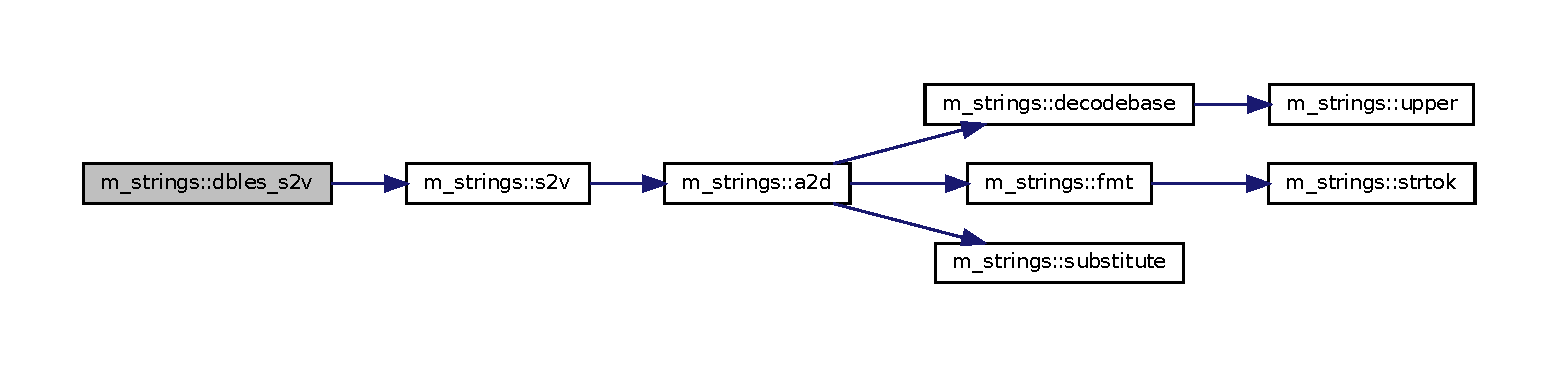
\includegraphics[width=350pt]{namespacem__strings_ab463f9b431dd817b7b509608ec823b0f_cgraph}
\end{center}
\end{figure}
\mbox{\Hypertarget{namespacem__strings_a3883dae1b85c2d4a09d2d7e46ff422ab}\label{namespacem__strings_a3883dae1b85c2d4a09d2d7e46ff422ab}} 
\index{m\+\_\+strings@{m\+\_\+strings}!decodebase@{decodebase}}
\index{decodebase@{decodebase}!m\+\_\+strings@{m\+\_\+strings}}
\subsubsection{\texorpdfstring{decodebase()}{decodebase()}}
{\footnotesize\ttfamily logical function, public m\+\_\+strings\+::decodebase (\begin{DoxyParamCaption}\item[{character(len=$\ast$), intent(in)}]{string,  }\item[{integer, intent(in)}]{basein,  }\item[{integer, intent(out)}]{out\+\_\+baseten }\end{DoxyParamCaption})}



\subsubsection*{N\+A\+ME}

decodebase(3f) -\/ \mbox{[}M\+\_\+strings\+:B\+A\+SE\mbox{]} convert whole number string in base \mbox{[}2-\/36\mbox{]} to base 10 number (L\+I\+C\+E\+N\+SE\+:PD)

\subsubsection*{S\+Y\+N\+O\+P\+S\+IS}

logical function decodebase(string,basein,out10)

character(len=$\ast$),intent(in) \+:\+: string integer,intent(in) \+:\+: basein integer,intent(out) \+:\+: out10 \subsubsection*{D\+E\+S\+C\+R\+I\+P\+T\+I\+ON}

\begin{DoxyVerb}Convert a numeric string representing a whole number in base BASEIN
to base 10. The function returns FALSE if BASEIN is not in the range
[2..36] or if string STRING contains invalid characters in base BASEIN
or if result OUT10 is too big

The letters A,B,...,Z represent 10,11,...,36 in the base > 10.
\end{DoxyVerb}


\subsubsection*{O\+P\+T\+I\+O\+NS}

string input string. It represents a whole number in the base specified by B\+A\+S\+E\+IN unless B\+A\+S\+E\+IN is set to zero. When B\+A\+S\+E\+IN is zero S\+T\+R\+I\+NG is assumed to be of the form B\+A\+S\+E\+::\+V\+A\+L\+UE where B\+A\+SE represents the function normally provided by B\+A\+S\+E\+IN. basein base of input string; either 0 or from 2 to 36. out10 output value in base 10

\subsubsection*{E\+X\+A\+M\+P\+LE}

Sample program\+: \begin{DoxyVerb}program demo_decodebase
use M_strings, only : codebase, decodebase
implicit none
integer           :: ba,bd
character(len=40) :: x,y
integer           :: r

print *,' BASE CONVERSION'
write(*,'("Start   Base (2 to 36): ")',advance='no'); read *, bd
write(*,'("Arrival Base (2 to 36): ")',advance='no'); read *, ba
INFINITE: do
   print *,''
   write(*,'("Enter number in start base: ")',advance='no'); read *, x
   if(x.eq.'0') exit INFINITE
   if(decodebase(x,bd,r)) then
      if(codebase(r,ba,y)) then
        write(*,'("In base ",I2,": ",A20)')  ba, y
      else
        print *,'Error in coding number.'
      endif
   else
      print *,'Error in decoding number.'
   endif
enddo INFINITE

end program demo_decodebase
\end{DoxyVerb}


\subsubsection*{A\+U\+T\+H\+OR}

John S. Urban

Ref.\+: "Math matiques en Turbo-\/\+Pascal by M. Ducamp and A. Reverchon (2), Eyrolles, Paris, 1988".

based on a F90 Version By J-\/P Moreau (www.\+jpmoreau.\+fr)

\subsubsection*{L\+I\+C\+E\+N\+SE}

Public Domain 

References upper().

Here is the call graph for this function\+:\nopagebreak
\begin{figure}[H]
\begin{center}
\leavevmode
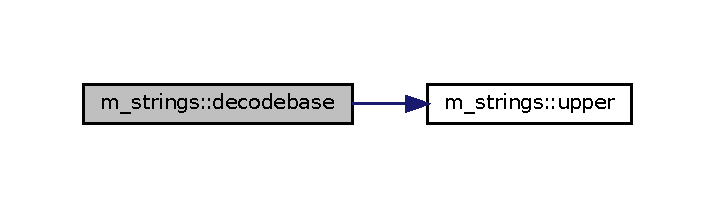
\includegraphics[width=343pt]{namespacem__strings_a3883dae1b85c2d4a09d2d7e46ff422ab_cgraph}
\end{center}
\end{figure}
Here is the caller graph for this function\+:\nopagebreak
\begin{figure}[H]
\begin{center}
\leavevmode
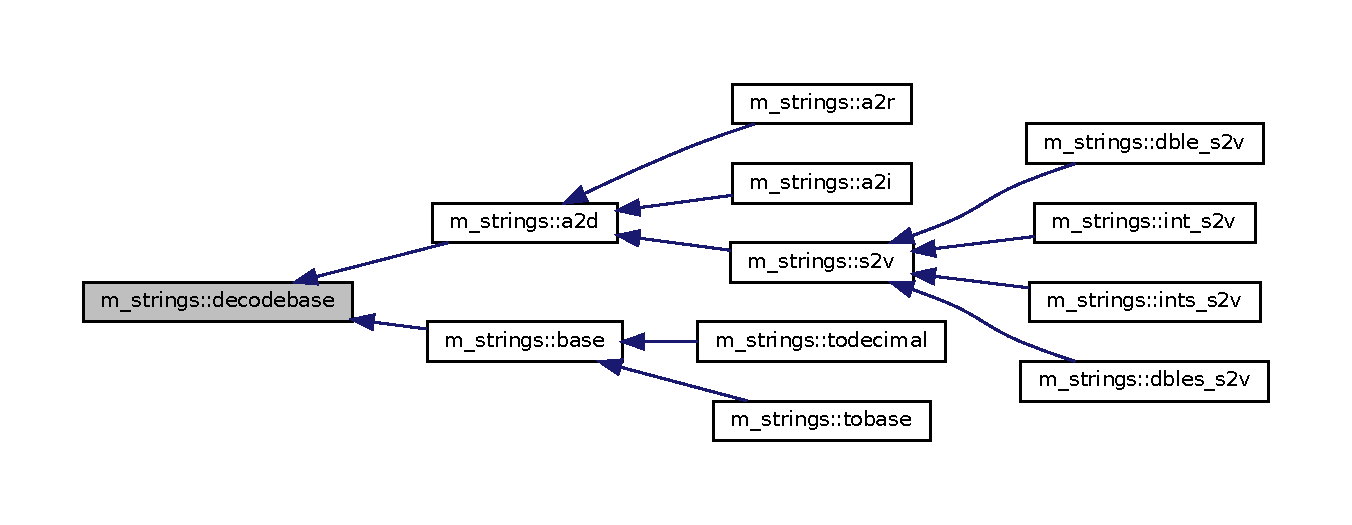
\includegraphics[width=350pt]{namespacem__strings_a3883dae1b85c2d4a09d2d7e46ff422ab_icgraph}
\end{center}
\end{figure}
\mbox{\Hypertarget{namespacem__strings_a9890da826d63d6f04367887007611cb5}\label{namespacem__strings_a9890da826d63d6f04367887007611cb5}} 
\index{m\+\_\+strings@{m\+\_\+strings}!delim@{delim}}
\index{delim@{delim}!m\+\_\+strings@{m\+\_\+strings}}
\subsubsection{\texorpdfstring{delim()}{delim()}}
{\footnotesize\ttfamily subroutine, public m\+\_\+strings\+::delim (\begin{DoxyParamCaption}\item[{character(len=$\ast$), intent(in)}]{line,  }\item[{character(len=$\ast$), dimension(n)}]{array,  }\item[{integer, intent(in)}]{n,  }\item[{integer, intent(out)}]{icount,  }\item[{integer, dimension(n), intent(out)}]{ibegin,  }\item[{integer, dimension(n), intent(out)}]{iterm,  }\item[{integer, intent(out)}]{ilen,  }\item[{character(len=$\ast$), intent(in)}]{dlim }\end{DoxyParamCaption})}



\subsubsection*{N\+A\+ME}

delim(3f) -\/ \mbox{[}M\+\_\+strings\+:T\+O\+K\+E\+NS\mbox{]} parse a string and store tokens into an array (L\+I\+C\+E\+N\+SE\+:PD) \subsubsection*{S\+Y\+N\+O\+P\+S\+IS}

subroutine delim(line,array,n,icount,ibegin,iterm,ilen,dlim)

character(len=$\ast$),intent(in) \+:\+: line integer,integer(in) \+:\+: n integer,intent(out) \+:\+: icount character(len=$\ast$) \+:\+: array(n) integer,intent(out) \+:\+: ibegin(n) integer,intent(out) \+:\+: iterm(n) integer,intent(out) \+:\+: ilen character(len=$\ast$) \+:\+: dlim \subsubsection*{D\+E\+S\+C\+R\+I\+P\+T\+I\+ON}

\begin{DoxyVerb}  Given a LINE of structure " par1 par2 par3 ... parn "
  store each par(n) into a separate variable in ARRAY (UNLESS
  ARRAY(1).eq.'#N#')

  Also set ICOUNT to number of elements of array initialized, and
  return beginning and ending positions for each element in IBEGIN(N)
  and ITERM(N).

  Return position of last non-blank character (even if more
  than N elements were found) in ILEN

  No quoting or escaping of delimiter is allowed, so the delimiter
  character can not be placed in a token.

  No checking for more than N parameters; If any more they are ignored.
\end{DoxyVerb}


\subsubsection*{O\+P\+T\+I\+O\+NS}

L\+I\+NE input string to parse into tokens A\+R\+R\+A\+Y(\+N) array that receives tokens N size of arrays A\+R\+R\+AY, I\+B\+E\+G\+IN, I\+T\+E\+RM I\+C\+O\+U\+NT number of tokens found I\+B\+E\+G\+I\+N(\+N) starting columns of tokens found I\+T\+E\+R\+M(\+N) ending columns of tokens found I\+L\+EN position of last non-\/blank character in input string L\+I\+NE D\+L\+IM delimiter characters

\subsubsection*{E\+X\+A\+M\+P\+L\+ES}

Sample program\+: \begin{DoxyVerb}program demo_delim

use M_strings, only: delim
character(len=80) :: line
character(len=80) :: dlm
integer,parameter :: n=10
character(len=20) :: array(n)=' '
integer           :: ibegin(n),iterm(n)
line=' first  second 10.3 words_of_stuff  '
do i20=1,4
   ! change delimiter list and what is calculated or parsed
   if(i20.eq.1)dlm=' '
   if(i20.eq.2)dlm='o'
   if(i20.eq.3)dlm=' aeiou'    ! NOTE SPACE IS FIRST
   if(i20.eq.3)ARRAY(1)='#N#'  ! QUIT RETURNING STRING ARRAY
   if(i20.eq.4)line='AAAaBBBBBBbIIIIIi  J K L'

   ! write out a break line composed of =========== ..
   write(*,'(57("="))')
   ! show line being parsed
   write(*,'(a)')'PARSING=['//trim(line)//'] on '//trim(dlm)
   ! call parsing procedure
   call delim(line,array,n,icount,ibegin,iterm,ilen,dlm)
   write(*,*)'number of tokens found=',icount
   write(*,*)'last character in column ',ilen
   if(icount.gt.0)then
      if(ilen.ne.iterm(icount))then
         write(*,*)'ignored from column ',iterm(icount)+1,' to ',ilen
      endif
      do i10=1,icount
         ! check flag to see if ARRAY() was set
         if(array(1).ne.'#N#')then
            ! from returned array
            write(*,'(a,a,a)',advance='no')&
            &'[',array(i10)(:iterm(i10)-ibegin(i10)+1),']'
         endif
      enddo
      ! using start and end positions in IBEGIN() and ITERM()
      write(*,*)
      do i10=1,icount
         ! from positions in original line
         write(*,'(a,a,a)',advance='no')&
         &'[',line(ibegin(i10):iterm(i10)),']'
      enddo
      write(*,*)
   endif
enddo
end program demo_delim
\end{DoxyVerb}


Expected output \subsubsection*{A\+U\+T\+H\+OR}

John S. Urban \subsubsection*{L\+I\+C\+E\+N\+SE}

Public Domain Here is the caller graph for this function\+:\nopagebreak
\begin{figure}[H]
\begin{center}
\leavevmode
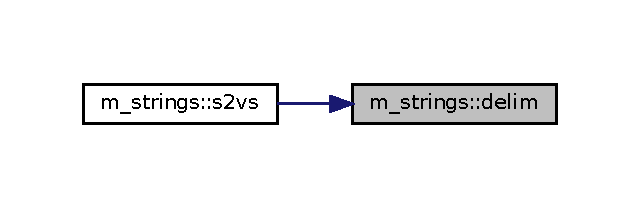
\includegraphics[width=307pt]{namespacem__strings_a9890da826d63d6f04367887007611cb5_icgraph}
\end{center}
\end{figure}
\mbox{\Hypertarget{namespacem__strings_a8d7007f0c34d7db4c004dac56e609b3f}\label{namespacem__strings_a8d7007f0c34d7db4c004dac56e609b3f}} 
\index{m\+\_\+strings@{m\+\_\+strings}!describe@{describe}}
\index{describe@{describe}!m\+\_\+strings@{m\+\_\+strings}}
\subsubsection{\texorpdfstring{describe()}{describe()}}
{\footnotesize\ttfamily character(len=\+:) function, allocatable, public m\+\_\+strings\+::describe (\begin{DoxyParamCaption}\item[{character(len=1), intent(in)}]{ch }\end{DoxyParamCaption})}



\subsubsection*{N\+A\+ME}

describe(3f) -\/ \mbox{[}M\+\_\+strings\mbox{]} returns a string describing the name of a single character (L\+I\+C\+E\+N\+SE\+:PD) 

\subsubsection*{S\+Y\+N\+O\+P\+S\+IS}

\begin{DoxyVerb}function describe(ch) result (string)

 character(len=1),intent(in)   :: ch
 character(len=:),allocatable  :: string
\end{DoxyVerb}
 \subsubsection*{D\+E\+S\+C\+R\+I\+P\+T\+I\+ON}

describe(3f) returns a string describing long name of a single character

\subsubsection*{E\+X\+A\+M\+P\+L\+ES}

Sample Program\+: \begin{DoxyVerb}program demo_describe
 use M_strings, only : describe
 implicit none
 integer :: i
    do i=1,128  ! fill variable with base ASCII character set
       write(*,*)describe(char(i-1))
    enddo
end program demo_describe
\end{DoxyVerb}


Expected output

ctrl-\/@ or ctrl-\/? (N\+UL) null ctrl-\/A (S\+OH) start of heading ctrl-\/B (S\+TX) start of text ctrl-\/C (E\+TX) end of text ctrl-\/D (E\+OT) end of transmission ctrl-\/E (E\+NQ) enquiry ctrl-\/F (A\+CK) acknowledge ctrl-\/G (B\+EL) bell ctrl-\/H (BS) backspace ctrl-\/I (HT) horizontal tabulation ctrl-\/J (LF) line feed ctrl-\/K (VT) vertical tabulation ctrl-\/L (FF) form feed ctrl-\/M (CR) carriage return ctrl-\/N (SO) shift out ctrl-\/O (SI) shift in ctrl-\/P (D\+LE) data link escape ctrl-\/Q (D\+C1) device control 1 ctrl-\/R (D\+C2) device control 2 ctrl-\/S (D\+C3) device control 3 ctrl-\/T (D\+C4) device control 4 ctrl-\/U (N\+AK) negative acknowledge ctrl-\/V (S\+YN) synchronous idle ctrl-\/W (E\+TB) end of transmission block ctrl-\/X (C\+AN) cancel ctrl-\/Y (EM) end of medium ctrl-\/Z (S\+UB) substitute ctrl-\/\mbox{[} (E\+SC) escape ctrl-\/\textbackslash{} or ctrl-\/@ (FS) file separator ctrl-\/\mbox{]} (GS) group separator ctrl-\/$^\wedge$ or ctrl-\/= (RS) record separator ctrl-\/\+\_\+ (US) unit separator space ! exclamation point " quotation marks \subsection*{number sign}

\$ currency symbol \% percent \& ampersand \textquotesingle{} apostrophe ( left parenthesis ) right parenthesis
\begin{DoxyItemize}
\item asterisk
\item plus , comma
\item minus . period / slash 0 zero 1 one 2 two 3 three 4 four 5 five 6 six 7 seven 8 eight 9 nine \+: colon ; semicolon $<$ less than = equals $>$ greater than ? question mark @ at sign majuscule A majuscule B majuscule C majuscule D majuscule E majuscule F majuscule G majuscule H majuscule I majuscule J majuscule K majuscule L majuscule M majuscule N majuscule O majuscule P majuscule Q majuscule R majuscule S majuscule T majuscule U majuscule V majuscule W majuscule X majuscule Y majuscule Z \mbox{[} left bracket \textbackslash{} backslash \mbox{]} right bracket $^\wedge$ caret \+\_\+ underscore \`{} grave accent miniscule a miniscule b miniscule c miniscule d miniscule e miniscule f miniscule g miniscule h miniscule i miniscule j miniscule k miniscule l miniscule m miniscule n miniscule o miniscule p miniscule q miniscule r miniscule s miniscule t miniscule u miniscule v miniscule w miniscule x miniscule y miniscule z \{ left brace $\vert$ vertical line \} right brace $\sim$ tilde ctrl-\/? (D\+EL) delete \subsubsection*{A\+U\+T\+H\+OR}
\end{DoxyItemize}

John S. Urban \subsubsection*{L\+I\+C\+E\+N\+SE}

Public Domain \mbox{\Hypertarget{namespacem__strings_a33b248107c1521272b55cda5c4077378}\label{namespacem__strings_a33b248107c1521272b55cda5c4077378}} 
\index{m\+\_\+strings@{m\+\_\+strings}!expand@{expand}}
\index{expand@{expand}!m\+\_\+strings@{m\+\_\+strings}}
\subsubsection{\texorpdfstring{expand()}{expand()}}
{\footnotesize\ttfamily character(len=\+:) function, allocatable, public m\+\_\+strings\+::expand (\begin{DoxyParamCaption}\item[{character(len=$\ast$)}]{line,  }\item[{character(len=1), intent(in), optional}]{escape }\end{DoxyParamCaption})}



\subsubsection*{N\+A\+ME}

expand(3f) -\/ \mbox{[}M\+\_\+strings\+:N\+O\+N\+A\+L\+P\+HA\mbox{]} expand C-\/like escape sequences (L\+I\+C\+E\+N\+SE\+:PD) 

\subsubsection*{S\+Y\+N\+O\+P\+S\+IS}

function expand(line,escape) result(lineout)

character(len=$\ast$) \+:\+: line character(len=1),intent(in),optional \+:\+: escape character(len=\+:),allocatable \+:\+: lineout \subsubsection*{D\+E\+S\+C\+R\+I\+P\+T\+I\+ON}

\begin{DoxyVerb}EXPAND() expands sequences used to represent commonly used escape sequences
or control characters. By default ...

 Escape sequences

   \      backslash
   a      alert (BEL) -- g is an alias for a
   b      backspace
   c      suppress further output
   e      escape
   f      form feed
   n      new line
   r      carriage return
   t      horizontal tab
   v      vertical tab
   oNNN   byte with octal value NNN (3 digits)
   dNNN   byte with decimal value NNN (3 digits)
   xHH    byte with hexadecimal value HH (2 digits) -- h is an alias for x

The default escape character is the backslash, but this may be changed using
the optional parameter ESCAPE.
\end{DoxyVerb}


\subsubsection*{E\+X\+A\+M\+P\+L\+ES}

Sample Program\+: \begin{DoxyVerb} program demo_expand
 !  test filter to expand escape sequences in input lines
 use M_strings, only : expand
 character(len=1024) :: line
 integer             :: ios
    READFILE: block
       do
          read(*,'(A)',iostat=ios)line
          if(ios /= 0) exit READFILE
          write(*,'(a)')trim(expand(line))
       enddo
    endblock READFILE
 end program demo_expand
\end{DoxyVerb}


Sample input\+: \begin{DoxyVerb}\e[2J
\tABC\tabc
\tA\a
\nONE\nTWO\nTHREE
\end{DoxyVerb}


\subsubsection*{A\+U\+T\+H\+OR}

John S. Urban \subsubsection*{L\+I\+C\+E\+N\+SE}

Public Domain \mbox{\Hypertarget{namespacem__strings_afccf1e453a4315a639f133f2f7c0078b}\label{namespacem__strings_afccf1e453a4315a639f133f2f7c0078b}} 
\index{m\+\_\+strings@{m\+\_\+strings}!fmt@{fmt}}
\index{fmt@{fmt}!m\+\_\+strings@{m\+\_\+strings}}
\subsubsection{\texorpdfstring{fmt()}{fmt()}}
{\footnotesize\ttfamily character(len=\+:) function, dimension(\+:), allocatable, public m\+\_\+strings\+::fmt (\begin{DoxyParamCaption}\item[{character(len=$\ast$), intent(in)}]{source\+\_\+string,  }\item[{integer, intent(in)}]{length }\end{DoxyParamCaption})}



\subsubsection*{N\+A\+ME}

fmt(3f) -\/ \mbox{[}M\+\_\+strings\+:T\+O\+K\+E\+NS\mbox{]} Tokenize a string, consuming it one token per call (L\+I\+C\+E\+N\+SE\+:PD) 

\subsubsection*{S\+Y\+N\+O\+P\+S\+IS}

function fmt(source\+\_\+string,length)

character(len=$\ast$),intent(in) \+:\+: source\+\_\+string integer,intent(in) \+:\+: length character(allocatable(len=length) \+:\+: fmt(\+:) \subsubsection*{D\+E\+S\+C\+R\+I\+P\+T\+I\+ON}

fmt(3f) breaks a long line into a simple paragraph of specified line length.

Given a long string break it on spaces into an array such that no variable is longer than the specified length. Individual words longer than L\+E\+N\+G\+TH will be placed in variables by themselves. \subsubsection*{O\+P\+T\+I\+O\+NS}

S\+O\+U\+R\+C\+E\+\_\+\+S\+T\+R\+I\+NG input string to break into an array of shorter strings on blank delimiters L\+E\+N\+G\+TH length of lines to break the string into. \subsubsection*{R\+E\+T\+U\+R\+NS}

F\+MT character array filled with data from source\+\_\+string broken at spaces into variables of length L\+E\+N\+G\+TH. \subsubsection*{E\+X\+A\+M\+P\+LE}

sample program \begin{DoxyVerb}program demo_fmt
use M_strings, only : fmt
character(len=80),allocatable :: paragraph(:)
character(len=*),parameter    :: string= '&
 &one two three four five &
 &six seven eight &
 &nine ten eleven twelve &
 &thirteen fourteen fifteen sixteen &
 &seventeen'

paragraph=fmt(string,40)
write(*,'(a)')paragraph

write(*,'(a)')fmt(string,0)
write(*,'(3x,a)')fmt(string,77)

end program demo_fmt
\end{DoxyVerb}


Results\+: \begin{DoxyVerb}one two three four five six seven eight
nine ten eleven twelve thirteen fourteen
fifteen sixteen seventeen
one
two
three
four
five
six
seven
eight
nine
ten
eleven
twelve
thirteen
fourteen
fifteen
sixteen
seventeen
   one two three four five six seven eight nine ten eleven twelve thirteen
   fourteen fifteen sixteen seventeen
\end{DoxyVerb}


\subsubsection*{A\+U\+T\+H\+OR}

John S. Urban \subsubsection*{L\+I\+C\+E\+N\+SE}

Public Domain 

References strtok().

Here is the call graph for this function\+:\nopagebreak
\begin{figure}[H]
\begin{center}
\leavevmode
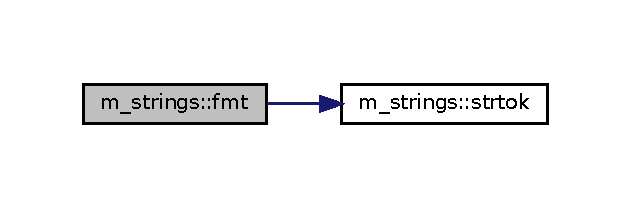
\includegraphics[width=303pt]{namespacem__strings_afccf1e453a4315a639f133f2f7c0078b_cgraph}
\end{center}
\end{figure}
Here is the caller graph for this function\+:\nopagebreak
\begin{figure}[H]
\begin{center}
\leavevmode
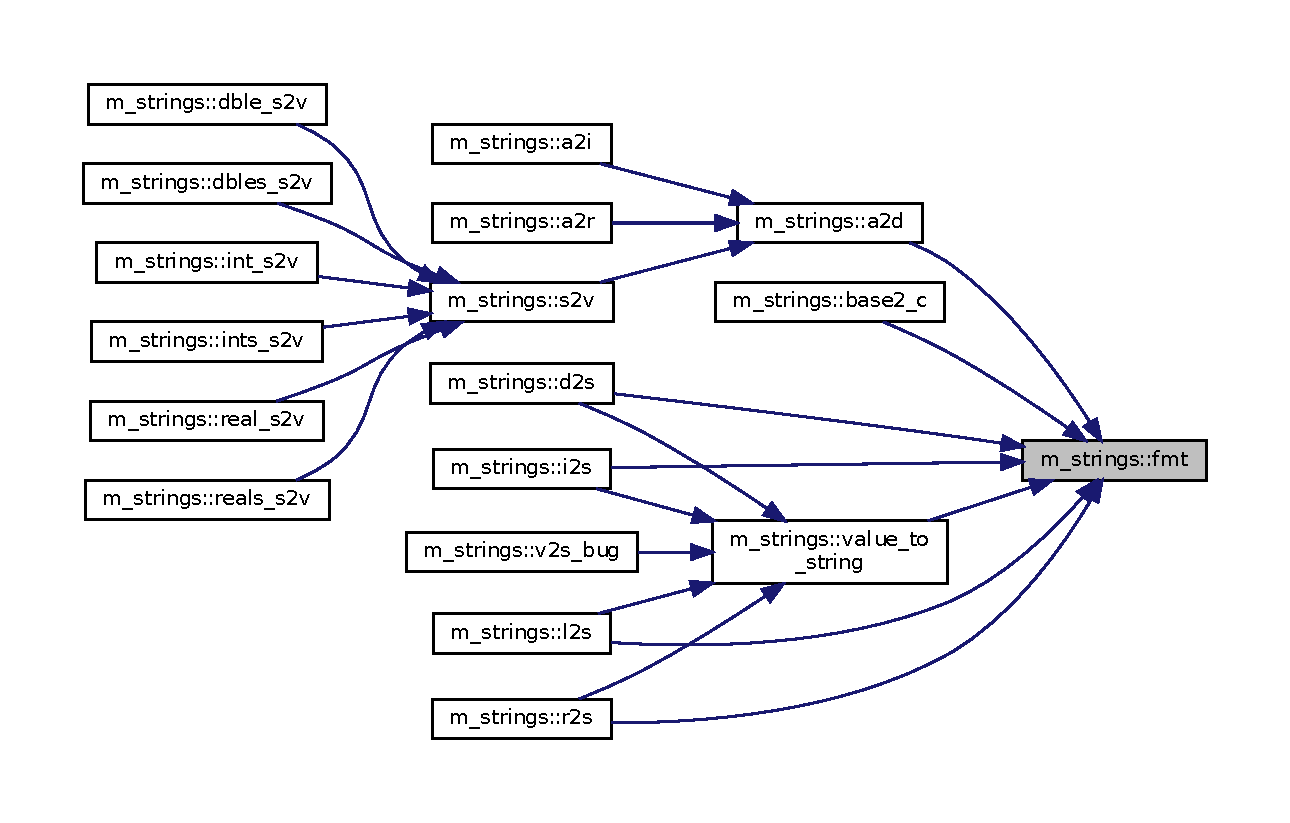
\includegraphics[width=350pt]{namespacem__strings_afccf1e453a4315a639f133f2f7c0078b_icgraph}
\end{center}
\end{figure}
\mbox{\Hypertarget{namespacem__strings_abf6c760f5d15a306bd252337d0a5ba4d}\label{namespacem__strings_abf6c760f5d15a306bd252337d0a5ba4d}} 
\index{m\+\_\+strings@{m\+\_\+strings}!getvals@{getvals}}
\index{getvals@{getvals}!m\+\_\+strings@{m\+\_\+strings}}
\subsubsection{\texorpdfstring{getvals()}{getvals()}}
{\footnotesize\ttfamily subroutine, public m\+\_\+strings\+::getvals (\begin{DoxyParamCaption}\item[{character(len=$\ast$), intent(in)}]{line,  }\item[{class($\ast$), dimension(\+:), intent(out)}]{values,  }\item[{integer, intent(out)}]{icount,  }\item[{integer, intent(out), optional}]{ierr }\end{DoxyParamCaption})}



\subsubsection*{N\+A\+ME}

getvals(3f) -\/ \mbox{[}M\+\_\+strings\+:N\+U\+M\+E\+R\+IC\mbox{]} read arbitrary number of R\+E\+AL values from a character variable up to size of V\+A\+L\+U\+E\+S() array (L\+I\+C\+E\+N\+SE\+:PD) 

\subsubsection*{S\+Y\+N\+O\+P\+S\+IS}

\begin{DoxyVerb}subroutine getvals(line,values,icount,ierr)

 character(len=*),intent(in)  :: line
 class(*),intent(out)         :: values(:)
 integer,intent(out)          :: icount
 integer,intent(out),optional :: ierr
\end{DoxyVerb}
 \subsubsection*{D\+E\+S\+C\+R\+I\+P\+T\+I\+ON}

G\+E\+T\+V\+A\+L\+S(3f) reads a relatively arbitrary number of numeric values from a character variable into a R\+E\+AL array using list-\/directed input.

N\+O\+TE\+: In this version null values are skipped instead of meaning to leave that value unchanged

1,,,,,,,2 / reads V\+A\+L\+U\+ES=\mbox{[}1.\+0,2.\+0\mbox{]}

Per list-\/directed rules when reading values, allowed delimiters are comma, semi-\/colon and space.

the slash separator can be used to add inline comments. \begin{DoxyVerb} 10.1, 20.43e-1 ; 11 / THIS IS TREATED AS A COMMENT
\end{DoxyVerb}


Repeat syntax can be used up to the size of the output array. These are equivalent input lines\+: \begin{DoxyVerb} 4*10.0
 10.0, 10.0, 10.0, 10.0
\end{DoxyVerb}


\subsubsection*{O\+P\+T\+I\+O\+NS}

L\+I\+NE A character variable containing the characters representing a list of numbers

\subsubsection*{R\+E\+T\+U\+R\+NS}

V\+A\+L\+U\+E\+S() array holding numbers read from string. May be of type I\+N\+T\+E\+G\+ER, R\+E\+AL, D\+O\+U\+B\+L\+E\+P\+R\+E\+C\+I\+S\+I\+ON, or C\+H\+A\+R\+A\+C\+T\+ER. If C\+H\+A\+R\+A\+C\+T\+ER the strings are returned as simple words instead of numeric values. I\+C\+O\+U\+NT number of defined numbers in V\+A\+L\+U\+E\+S(). If I\+C\+O\+U\+NT reaches the size of the V\+A\+L\+U\+E\+S() array parsing stops. I\+E\+RR zero if no error occurred in reading numbers. Optional. If not present and an error occurs the program is terminated.

\subsubsection*{E\+X\+A\+M\+P\+L\+ES}

Sample program\+: \begin{DoxyVerb}program demo_getvals
use M_strings, only: getvals
implicit none
integer,parameter  :: longest_line=256
character(len=longest_line) :: line
real               :: values(longest_line/2+1)
integer            :: ios,icount,ierr
INFINITE: do
   read(*,'(a)',iostat=ios) line
   if(ios.ne.0)exit INFINITE
   call getvals(line,values,icount,ierr)
   write(*,*)'VALUES=',values(:icount)
enddo INFINITE
end program demo_getvals
\end{DoxyVerb}


Sample input lines \begin{DoxyVerb} 10,20 30.4
 1 2 3
 1

 3 4*2.5 8
 32.3333 / comment 1
 30e3;300,    30.0, 3
 even 1 like this! 10
 11,,,,22,,,,33
\end{DoxyVerb}


Expected output\+: \begin{DoxyVerb}VALUES=   10.0000000       20.0000000       30.3999996
VALUES=   1.00000000       2.00000000       3.00000000
VALUES=   1.00000000
VALUES=
VALUES=   3.00000000       2.50000000       2.50000000       2.50000000       2.50000000       8.00000000
VALUES=   32.3333015
VALUES=   30000.0000       300.000000       30.0000000       3.00000000
*getvals* WARNING:[even] is not a number
*getvals* WARNING:[like] is not a number
*getvals* WARNING:[this!] is not a number
VALUES=   1.00000000       10.0000000
VALUES=   11.0000000       22.0000000       33.0000000
\end{DoxyVerb}


\subsubsection*{A\+U\+T\+H\+OR}

John S. Urban \subsubsection*{L\+I\+C\+E\+N\+SE}

Public Domain \mbox{\Hypertarget{namespacem__strings_a76d3a650fbfec1f65d8fd81042347408}\label{namespacem__strings_a76d3a650fbfec1f65d8fd81042347408}} 
\index{m\+\_\+strings@{m\+\_\+strings}!i2s@{i2s}}
\index{i2s@{i2s}!m\+\_\+strings@{m\+\_\+strings}}
\subsubsection{\texorpdfstring{i2s()}{i2s()}}
{\footnotesize\ttfamily character(len=\+:) function, allocatable, private m\+\_\+strings\+::i2s (\begin{DoxyParamCaption}\item[{integer, intent(in)}]{ivalue,  }\item[{character(len=$\ast$), intent(in), optional}]{fmt }\end{DoxyParamCaption})\hspace{0.3cm}{\ttfamily [private]}}



References fmt(), and value\+\_\+to\+\_\+string().

Here is the call graph for this function\+:\nopagebreak
\begin{figure}[H]
\begin{center}
\leavevmode
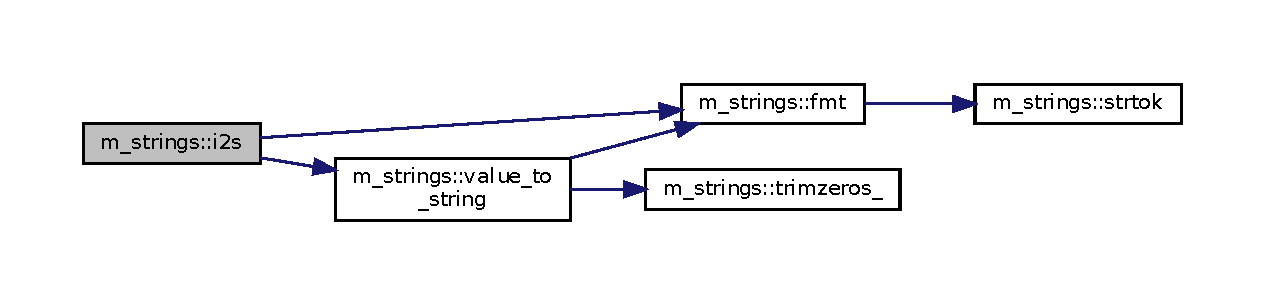
\includegraphics[width=350pt]{namespacem__strings_a76d3a650fbfec1f65d8fd81042347408_cgraph}
\end{center}
\end{figure}
\mbox{\Hypertarget{namespacem__strings_a020dcca7f01d33eedf28b17518a22b69}\label{namespacem__strings_a020dcca7f01d33eedf28b17518a22b69}} 
\index{m\+\_\+strings@{m\+\_\+strings}!indent@{indent}}
\index{indent@{indent}!m\+\_\+strings@{m\+\_\+strings}}
\subsubsection{\texorpdfstring{indent()}{indent()}}
{\footnotesize\ttfamily integer function, public m\+\_\+strings\+::indent (\begin{DoxyParamCaption}\item[{character(len=$\ast$), intent(in)}]{line }\end{DoxyParamCaption})}



\subsubsection*{N\+A\+ME}

indent(3f) -\/ \mbox{[}M\+\_\+strings\+:W\+H\+I\+T\+E\+S\+P\+A\+CE\mbox{]} count number of leading spaces in a string (L\+I\+C\+E\+N\+SE\+:PD) 

\subsubsection*{S\+Y\+N\+O\+P\+S\+IS}

\begin{DoxyVerb}function indent(line)

 integer                        :: indent
 character(len=*),intent(in)    :: line
\end{DoxyVerb}
 \subsubsection*{D\+E\+S\+C\+R\+I\+P\+T\+I\+ON}

Count number of leading spaces in a C\+H\+A\+R\+A\+C\+T\+ER variable.

\subsubsection*{E\+X\+A\+M\+P\+L\+ES}

Sample Program\+: \begin{DoxyVerb} program demo_indent
 !  test filter to count leading spaces in a character variable
 !  might want to call notabs(3f) to expand tab characters
 use M_strings, only : indent
 implicit none
 character(len=1024) :: in
 integer             :: ios
    READFILE: do
       read(*,'(A)',iostat=ios)in
       if(ios /= 0) exit READFILE
       write(*,'(i3,"",a)')indent(in),trim(in)
    enddo READFILE
 end program demo_indent
\end{DoxyVerb}


\subsubsection*{A\+U\+T\+H\+OR}

John S. Urban \subsubsection*{L\+I\+C\+E\+N\+SE}

Public Domain \mbox{\Hypertarget{namespacem__strings_aa94164439fc7659e175cf639e7315c0d}\label{namespacem__strings_aa94164439fc7659e175cf639e7315c0d}} 
\index{m\+\_\+strings@{m\+\_\+strings}!int\+\_\+s2v@{int\+\_\+s2v}}
\index{int\+\_\+s2v@{int\+\_\+s2v}!m\+\_\+strings@{m\+\_\+strings}}
\subsubsection{\texorpdfstring{int\+\_\+s2v()}{int\_s2v()}}
{\footnotesize\ttfamily integer function m\+\_\+strings\+::int\+\_\+s2v (\begin{DoxyParamCaption}\item[{character(len=$\ast$), intent(in)}]{chars }\end{DoxyParamCaption})\hspace{0.3cm}{\ttfamily [private]}}



References s2v().

Here is the call graph for this function\+:\nopagebreak
\begin{figure}[H]
\begin{center}
\leavevmode
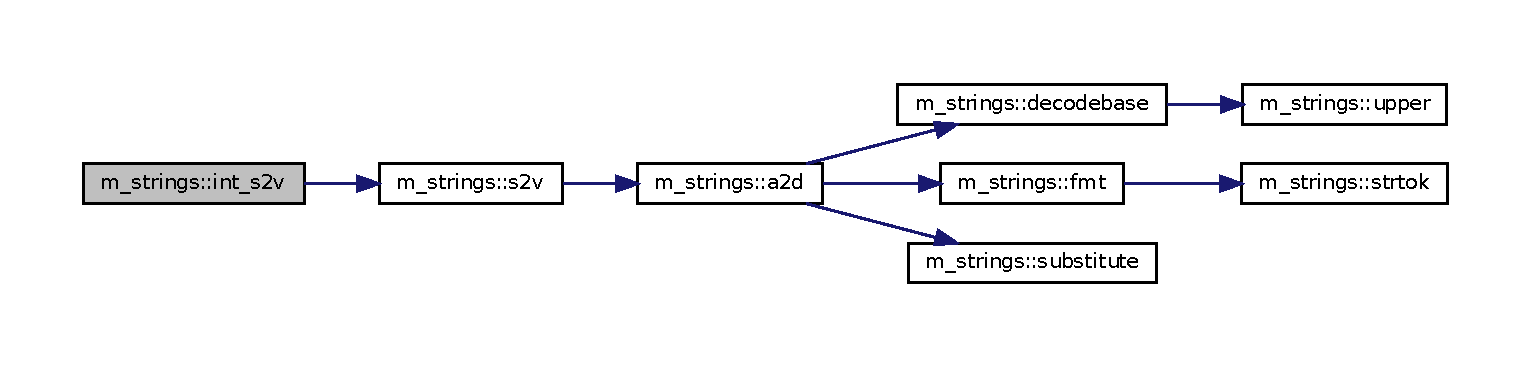
\includegraphics[width=350pt]{namespacem__strings_aa94164439fc7659e175cf639e7315c0d_cgraph}
\end{center}
\end{figure}
\mbox{\Hypertarget{namespacem__strings_a4e54d205168cab37d25119d74a9ead63}\label{namespacem__strings_a4e54d205168cab37d25119d74a9ead63}} 
\index{m\+\_\+strings@{m\+\_\+strings}!ints\+\_\+s2v@{ints\+\_\+s2v}}
\index{ints\+\_\+s2v@{ints\+\_\+s2v}!m\+\_\+strings@{m\+\_\+strings}}
\subsubsection{\texorpdfstring{ints\+\_\+s2v()}{ints\_s2v()}}
{\footnotesize\ttfamily integer function, dimension(\+:), allocatable m\+\_\+strings\+::ints\+\_\+s2v (\begin{DoxyParamCaption}\item[{character(len=$\ast$), dimension(\+:), intent(in)}]{chars }\end{DoxyParamCaption})\hspace{0.3cm}{\ttfamily [private]}}



References s2v().

Here is the call graph for this function\+:\nopagebreak
\begin{figure}[H]
\begin{center}
\leavevmode
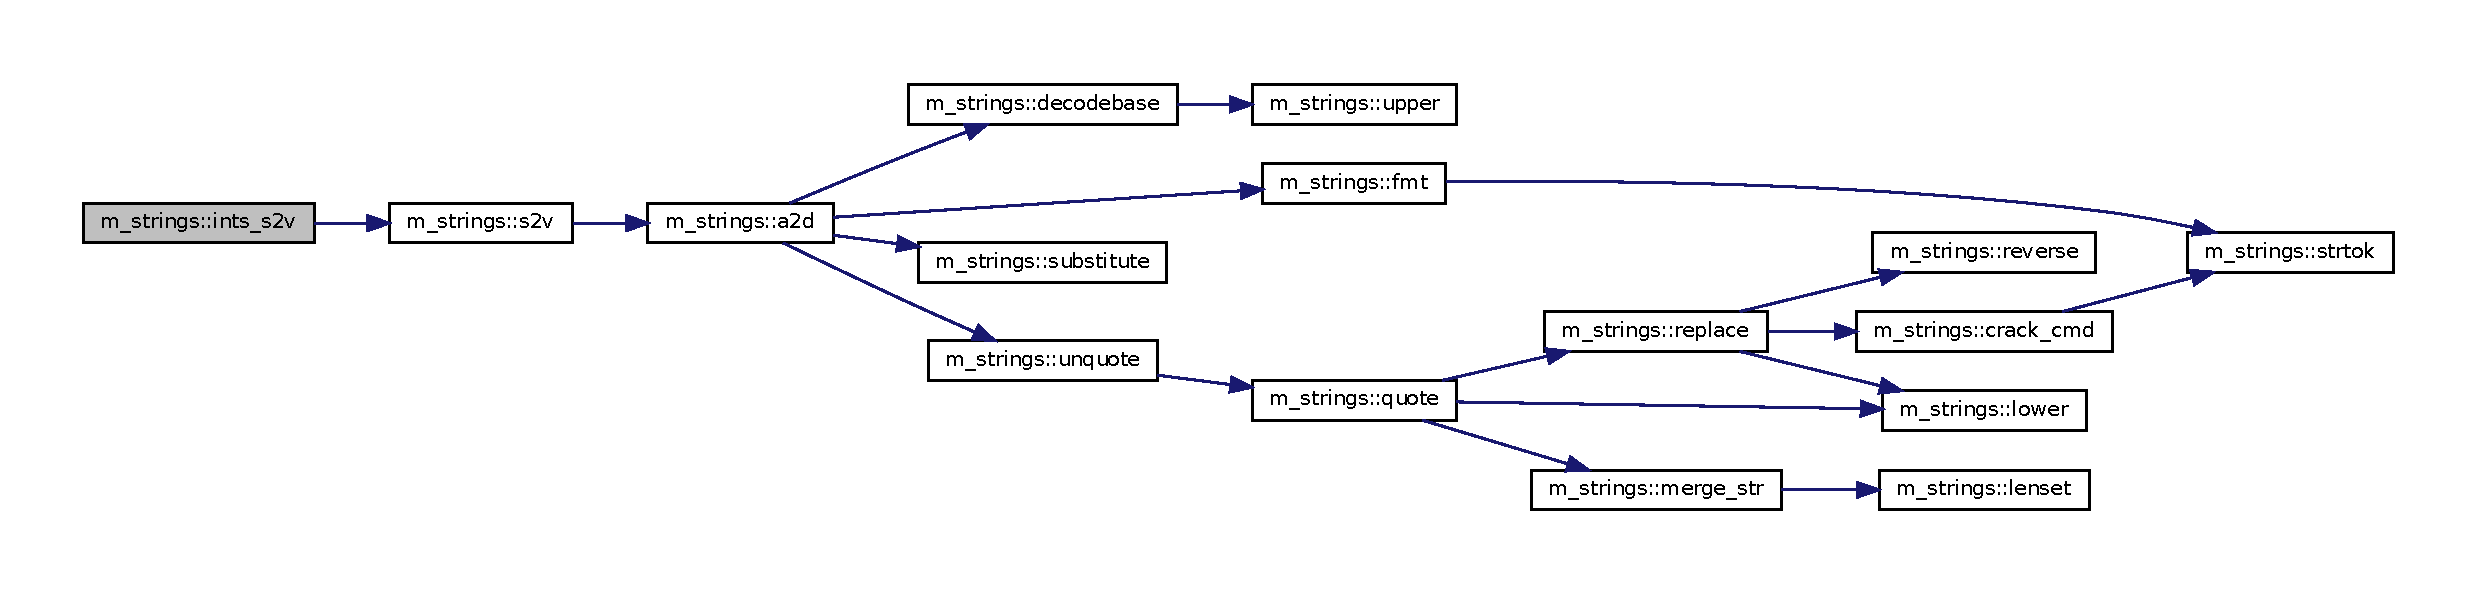
\includegraphics[width=350pt]{namespacem__strings_a4e54d205168cab37d25119d74a9ead63_cgraph}
\end{center}
\end{figure}
\mbox{\Hypertarget{namespacem__strings_ad8fd9bbf618bdba2c3ac9fb3c8174362}\label{namespacem__strings_ad8fd9bbf618bdba2c3ac9fb3c8174362}} 
\index{m\+\_\+strings@{m\+\_\+strings}!isalnum@{isalnum}}
\index{isalnum@{isalnum}!m\+\_\+strings@{m\+\_\+strings}}
\subsubsection{\texorpdfstring{isalnum()}{isalnum()}}
{\footnotesize\ttfamily elemental logical function, public m\+\_\+strings\+::isalnum (\begin{DoxyParamCaption}\item[{character, intent(in)}]{ch }\end{DoxyParamCaption})}



\subsubsection*{N\+A\+ME}

isalnum,isalpha,iscntrl,isdigit,isgraph,islower, isprint,ispunct,isspace,isupper,isascii,isblank,isxdigit(3f) -\/ \mbox{[}M\+\_\+strings\+:C\+O\+M\+P\+A\+RE\mbox{]} test membership in subsets of A\+S\+C\+II set (L\+I\+C\+E\+N\+SE\+:PD) 

\subsubsection*{S\+Y\+N\+O\+P\+S\+IS}

\begin{DoxyVerb}Where "FUNCNAME" is one of the function names in the group, the functions are defined by

 elemental function FUNCNAME(onechar)
 character,intent(in) :: onechar
 logical              :: FUNC_NAME
\end{DoxyVerb}
 \subsubsection*{D\+E\+S\+C\+R\+I\+P\+T\+I\+ON}

\begin{DoxyVerb}These elemental functions test if a character belongs to various subsets of the ASCII character set.

    isalnum    returns .true. if character is a letter (a-z,A-Z) or digit (0-9)
    isalpha    returns .true. if character is a letter and .false. otherwise
    isascii    returns .true. if character is in the range char(0) to char(127)
    isblank    returns .true. if character is a blank (space or horizontal tab).
    iscntrl    returns .true. if character is a delete character or ordinary control character (0x7F or 0x00-0x1F).
    isdigit    returns .true. if character is a digit (0,1,...,9) and .false. otherwise
    isgraph    returns .true. if character is a printable ASCII character excluding space
    islower    returns .true. if character is a miniscule letter (a-z)
    isprint    returns .true. if character is a printable ASCII character
    ispunct    returns .true. if character is a printable punctuation character (isgraph(c) && !isalnum(c)).
    isspace    returns .true. if character is a null, space, tab, carriage return, new line, vertical tab, or formfeed
    isupper    returns .true. if character is an uppercase letter (A-Z)
    isxdigit   returns .true. if character is a hexadecimal digit (0-9, a-f, or A-F).
\end{DoxyVerb}


\subsubsection*{E\+X\+A\+M\+P\+L\+ES}

Sample Program\+:

program demo\+\_\+isdigit \begin{DoxyVerb} use M_strings, only : isdigit, isspace, switch
 implicit none
 character(len=10),allocatable :: string(:)
 integer                       :: i
    string=[&
    & '1 2 3 4 5 ' ,&
    & 'letters   ' ,&
    & '1234567890' ,&
    & 'both 8787 ' ]
    ! if string is nothing but digits and whitespace return .true.
    do i=1,size(string)
       write(*,'(a)',advance='no')'For string['//string(i)//']'
       write(*,*) &
       all(isdigit(switch(string(i))).or.isspace(switch(string(i))))
    enddo

 end program demo_isdigit
\end{DoxyVerb}


Expected output\+: \begin{DoxyVerb}For string[1 2 3 4 5 ] T
For string[letters   ] F
For string[1234567890] T
For string[both 8787 ] F
\end{DoxyVerb}


\subsubsection*{A\+U\+T\+H\+OR}

John S. Urban \subsubsection*{L\+I\+C\+E\+N\+SE}

Public Domain \mbox{\Hypertarget{namespacem__strings_a5cf6d7fbd1b3ea17e37c6213c6ba0fdb}\label{namespacem__strings_a5cf6d7fbd1b3ea17e37c6213c6ba0fdb}} 
\index{m\+\_\+strings@{m\+\_\+strings}!isalpha@{isalpha}}
\index{isalpha@{isalpha}!m\+\_\+strings@{m\+\_\+strings}}
\subsubsection{\texorpdfstring{isalpha()}{isalpha()}}
{\footnotesize\ttfamily elemental logical function, public m\+\_\+strings\+::isalpha (\begin{DoxyParamCaption}\item[{character, intent(in)}]{ch }\end{DoxyParamCaption})}

\mbox{\Hypertarget{namespacem__strings_afb63e9fefbc04e4e9a2ec4df4334078c}\label{namespacem__strings_afb63e9fefbc04e4e9a2ec4df4334078c}} 
\index{m\+\_\+strings@{m\+\_\+strings}!isascii@{isascii}}
\index{isascii@{isascii}!m\+\_\+strings@{m\+\_\+strings}}
\subsubsection{\texorpdfstring{isascii()}{isascii()}}
{\footnotesize\ttfamily elemental logical function, public m\+\_\+strings\+::isascii (\begin{DoxyParamCaption}\item[{character, intent(in)}]{ch }\end{DoxyParamCaption})}

\mbox{\Hypertarget{namespacem__strings_aebb074d3971c0b93e39d1cfaa45658d8}\label{namespacem__strings_aebb074d3971c0b93e39d1cfaa45658d8}} 
\index{m\+\_\+strings@{m\+\_\+strings}!isblank@{isblank}}
\index{isblank@{isblank}!m\+\_\+strings@{m\+\_\+strings}}
\subsubsection{\texorpdfstring{isblank()}{isblank()}}
{\footnotesize\ttfamily elemental logical function, public m\+\_\+strings\+::isblank (\begin{DoxyParamCaption}\item[{character, intent(in)}]{ch }\end{DoxyParamCaption})}

\mbox{\Hypertarget{namespacem__strings_a4821cb5a5c4024c9dc6dd159300034ca}\label{namespacem__strings_a4821cb5a5c4024c9dc6dd159300034ca}} 
\index{m\+\_\+strings@{m\+\_\+strings}!iscntrl@{iscntrl}}
\index{iscntrl@{iscntrl}!m\+\_\+strings@{m\+\_\+strings}}
\subsubsection{\texorpdfstring{iscntrl()}{iscntrl()}}
{\footnotesize\ttfamily elemental logical function, public m\+\_\+strings\+::iscntrl (\begin{DoxyParamCaption}\item[{character, intent(in)}]{ch }\end{DoxyParamCaption})}

\mbox{\Hypertarget{namespacem__strings_a9f5f98a6c93e21618a16d98a5de2debc}\label{namespacem__strings_a9f5f98a6c93e21618a16d98a5de2debc}} 
\index{m\+\_\+strings@{m\+\_\+strings}!isdigit@{isdigit}}
\index{isdigit@{isdigit}!m\+\_\+strings@{m\+\_\+strings}}
\subsubsection{\texorpdfstring{isdigit()}{isdigit()}}
{\footnotesize\ttfamily elemental logical function, public m\+\_\+strings\+::isdigit (\begin{DoxyParamCaption}\item[{character, intent(in)}]{ch }\end{DoxyParamCaption})}

Here is the caller graph for this function\+:\nopagebreak
\begin{figure}[H]
\begin{center}
\leavevmode
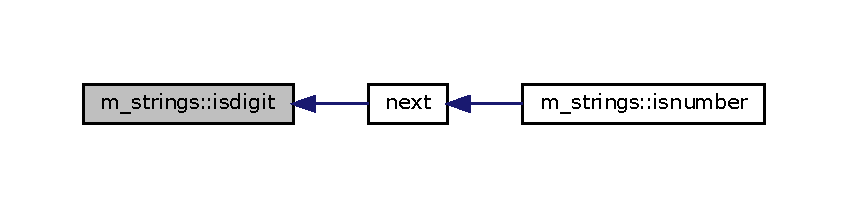
\includegraphics[width=350pt]{namespacem__strings_a9f5f98a6c93e21618a16d98a5de2debc_icgraph}
\end{center}
\end{figure}
\mbox{\Hypertarget{namespacem__strings_a84c80fdeeba0679488ed8ad8d37e53c5}\label{namespacem__strings_a84c80fdeeba0679488ed8ad8d37e53c5}} 
\index{m\+\_\+strings@{m\+\_\+strings}!isgraph@{isgraph}}
\index{isgraph@{isgraph}!m\+\_\+strings@{m\+\_\+strings}}
\subsubsection{\texorpdfstring{isgraph()}{isgraph()}}
{\footnotesize\ttfamily elemental logical function, public m\+\_\+strings\+::isgraph (\begin{DoxyParamCaption}\item[{character, intent(in)}]{onechar }\end{DoxyParamCaption})}

\mbox{\Hypertarget{namespacem__strings_a9de5290748f02f575f3b7b859ff074ed}\label{namespacem__strings_a9de5290748f02f575f3b7b859ff074ed}} 
\index{m\+\_\+strings@{m\+\_\+strings}!islower@{islower}}
\index{islower@{islower}!m\+\_\+strings@{m\+\_\+strings}}
\subsubsection{\texorpdfstring{islower()}{islower()}}
{\footnotesize\ttfamily elemental logical function, public m\+\_\+strings\+::islower (\begin{DoxyParamCaption}\item[{character, intent(in)}]{ch }\end{DoxyParamCaption})}

\mbox{\Hypertarget{namespacem__strings_a2b6c57cbc52fc86d2f02d0936d3484af}\label{namespacem__strings_a2b6c57cbc52fc86d2f02d0936d3484af}} 
\index{m\+\_\+strings@{m\+\_\+strings}!isnumber@{isnumber}}
\index{isnumber@{isnumber}!m\+\_\+strings@{m\+\_\+strings}}
\subsubsection{\texorpdfstring{isnumber()}{isnumber()}}
{\footnotesize\ttfamily integer function, public m\+\_\+strings\+::isnumber (\begin{DoxyParamCaption}\item[{character(len=$\ast$), intent(in)}]{string,  }\item[{character(len=\+:), intent(out), optional, allocatable}]{msg,  }\item[{logical, intent(in), optional}]{verbose }\end{DoxyParamCaption})}



\subsubsection*{N\+A\+ME}

isnumber(3f) -\/ \mbox{[}M\+\_\+strings\+:N\+U\+M\+E\+R\+IC\mbox{]} determine if a string represents a number (L\+I\+C\+E\+N\+SE\+:PD) \subsubsection*{S\+Y\+N\+O\+P\+S\+IS}

function isnumber(str,msg)

character(len=$\ast$),intent(in) \+:\+: str character(len=\+:),intent(out),allocatable,optional \+:\+: msg \subsubsection*{D\+E\+S\+C\+R\+I\+P\+T\+I\+ON}

I\+S\+N\+U\+M\+B\+E\+R(3f) returns a value greater than zero if the string represents a number, and a number less than or equal to zero if it is a bad number. Blank characters are ignored. \subsubsection*{O\+P\+T\+I\+O\+NS}

str the string to evaluate as to whether it represents a numeric value or not msg An optional message describing the string \subsubsection*{R\+E\+T\+U\+R\+NS}

isnumber the following values are returned \begin{DoxyVerb}       1 for an integer             [-+]NNNNN
       2 for a whole number         [-+]NNNNN.
       3 for a real value           [-+]NNNNN.MMMM
       4 for a exponential value    [-+]NNNNN.MMMM[-+]LLLL
                                    [-+]NNNNN.MMMM[ed][-+]LLLL

      values less than 1 represent an error
\end{DoxyVerb}


\subsubsection*{E\+X\+A\+M\+P\+L\+ES}

As the example shows, you can use an internal R\+E\+A\+D(3f) along with the I\+O\+S\+T\+AT= parameter to check (and read) a string as well. \begin{DoxyVerb} program demo_isnumber
 use M_strings, only : isnumber
 implicit none
 character(len=256) :: line
 real               :: value
 integer            :: ios
 integer            :: answer
 character(len=256) :: message
 character(len=:),allocatable :: description
    write(*,*)'Begin entering values, one per line'
    do
       read(*,'(a)',iostat=ios)line
       !
       ! try string as number using list-directed input
       line=''
       read(line,*,iostat=ios,iomsg=message) value
       if(ios.eq.0)then
          write(*,*)'VALUE=',value
       else
          write(*,*)'ERROR:',ios,trim(message)
       endif
       !
       ! try string using isnumber(3f)
       answer=isnumber(line,msg=description)
       if(answer.gt.0)then
          write(*,*)' for ',trim(line),' ',answer,':',description
       else
          write(*,*)' ERROR for ',trim(line),' ',answer,':',description
       endif
       !
    enddo
 end program demo_isnumber
\end{DoxyVerb}


Example run

$>$ Begin entering values $>$ E\+R\+R\+OR\+: -\/1 End of file $>$ E\+R\+R\+OR for -\/1 \+:null string $>$10 $>$ V\+A\+L\+UE= 10.\+0000000 $>$ for 10 1 \+:integer $>$20 $>$ V\+A\+L\+UE= 20.\+0000000 $>$ for 20 1 \+:integer $>$20. $>$ V\+A\+L\+UE= 20.\+0000000 $>$ for 20. 2 \+:whole number $>$30.\+1 $>$ V\+A\+L\+UE= 30.\+1000004 $>$ for 30.\+1 3 \+:real number $>$3e1 $>$ V\+A\+L\+UE= 30.\+0000000 $>$ for 3e1 4 \+:value with exponent $>$1-\/2 $>$ V\+A\+L\+UE= 9.\+99999978E-\/03 $>$ for 1-\/2 4 \+:value with exponent $>$100.\+22d-\/4 $>$ V\+A\+L\+UE= 1.\+00220004E-\/02 $>$ for 100.\+22d-\/4 4 \+:value with exponent $>$1--2 $>$ E\+R\+R\+OR\+: 5010 Bad real number in item 1 of list input $>$ E\+R\+R\+OR for 1--2 -\/5 \+:bad number $>$e $>$ E\+R\+R\+OR\+: 5010 Bad real number in item 1 of list input $>$ E\+R\+R\+OR for e -\/6 \+:missing leading value before exponent $>$e1 $>$ E\+R\+R\+OR\+: 5010 Bad real number in item 1 of list input $>$ E\+R\+R\+OR for e1 -\/6 \+:missing leading value before exponent $>$1e $>$ E\+R\+R\+OR\+: 5010 Bad real number in item 1 of list input $>$ E\+R\+R\+OR for 1e -\/3 \+:missing exponent $>$1e+ $>$ E\+R\+R\+OR\+: 5010 Bad real number in item 1 of list input $>$ E\+R\+R\+OR for 1e+ -\/4 \+:missing exponent after sign $>$1e+2.0 $>$ E\+R\+R\+OR\+: 5010 Bad real number in item 1 of list input $>$ E\+R\+R\+OR for 1e+2.0 -\/5 \+:bad number \subsubsection*{A\+U\+T\+H\+OR}

John S. Urban \subsubsection*{L\+I\+C\+E\+N\+SE}

Public Domain 

References next(), and nospace().

Here is the call graph for this function\+:\nopagebreak
\begin{figure}[H]
\begin{center}
\leavevmode
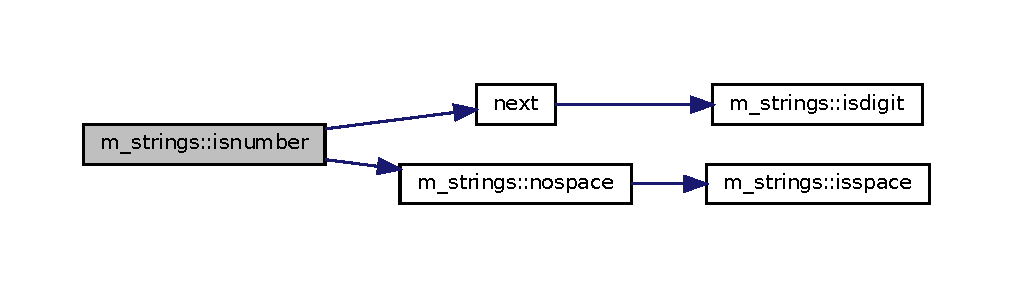
\includegraphics[width=350pt]{namespacem__strings_a2b6c57cbc52fc86d2f02d0936d3484af_cgraph}
\end{center}
\end{figure}
\mbox{\Hypertarget{namespacem__strings_a267f2fde729a75496c82a64754a91e54}\label{namespacem__strings_a267f2fde729a75496c82a64754a91e54}} 
\index{m\+\_\+strings@{m\+\_\+strings}!isprint@{isprint}}
\index{isprint@{isprint}!m\+\_\+strings@{m\+\_\+strings}}
\subsubsection{\texorpdfstring{isprint()}{isprint()}}
{\footnotesize\ttfamily elemental logical function, public m\+\_\+strings\+::isprint (\begin{DoxyParamCaption}\item[{character, intent(in)}]{onechar }\end{DoxyParamCaption})}

\mbox{\Hypertarget{namespacem__strings_a8712164e1f5fd717bdea854a3f067619}\label{namespacem__strings_a8712164e1f5fd717bdea854a3f067619}} 
\index{m\+\_\+strings@{m\+\_\+strings}!ispunct@{ispunct}}
\index{ispunct@{ispunct}!m\+\_\+strings@{m\+\_\+strings}}
\subsubsection{\texorpdfstring{ispunct()}{ispunct()}}
{\footnotesize\ttfamily elemental logical function, public m\+\_\+strings\+::ispunct (\begin{DoxyParamCaption}\item[{character, intent(in)}]{ch }\end{DoxyParamCaption})}

\mbox{\Hypertarget{namespacem__strings_ab32380c29451e56395153155c1632d74}\label{namespacem__strings_ab32380c29451e56395153155c1632d74}} 
\index{m\+\_\+strings@{m\+\_\+strings}!isspace@{isspace}}
\index{isspace@{isspace}!m\+\_\+strings@{m\+\_\+strings}}
\subsubsection{\texorpdfstring{isspace()}{isspace()}}
{\footnotesize\ttfamily elemental logical function, public m\+\_\+strings\+::isspace (\begin{DoxyParamCaption}\item[{character, intent(in)}]{ch }\end{DoxyParamCaption})}

Here is the caller graph for this function\+:
\nopagebreak
\begin{figure}[H]
\begin{center}
\leavevmode
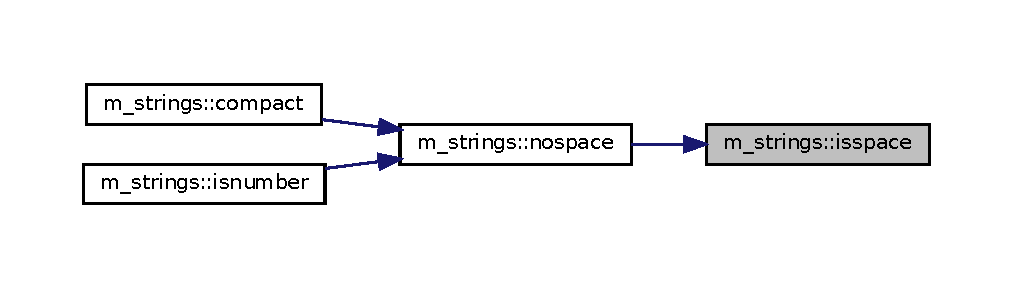
\includegraphics[width=350pt]{namespacem__strings_ab32380c29451e56395153155c1632d74_icgraph}
\end{center}
\end{figure}
\mbox{\Hypertarget{namespacem__strings_ac98536a1b69026cd5373dfff489f7733}\label{namespacem__strings_ac98536a1b69026cd5373dfff489f7733}} 
\index{m\+\_\+strings@{m\+\_\+strings}!isupper@{isupper}}
\index{isupper@{isupper}!m\+\_\+strings@{m\+\_\+strings}}
\subsubsection{\texorpdfstring{isupper()}{isupper()}}
{\footnotesize\ttfamily pure elemental logical function, public m\+\_\+strings\+::isupper (\begin{DoxyParamCaption}\item[{character, intent(in)}]{ch }\end{DoxyParamCaption})}

\mbox{\Hypertarget{namespacem__strings_a9953d1e400bedceab6a06910c6cdf208}\label{namespacem__strings_a9953d1e400bedceab6a06910c6cdf208}} 
\index{m\+\_\+strings@{m\+\_\+strings}!isxdigit@{isxdigit}}
\index{isxdigit@{isxdigit}!m\+\_\+strings@{m\+\_\+strings}}
\subsubsection{\texorpdfstring{isxdigit()}{isxdigit()}}
{\footnotesize\ttfamily elemental logical function, public m\+\_\+strings\+::isxdigit (\begin{DoxyParamCaption}\item[{character, intent(in)}]{ch }\end{DoxyParamCaption})}

\mbox{\Hypertarget{namespacem__strings_a36c4cc6f83b736b4e337a1289694e3d6}\label{namespacem__strings_a36c4cc6f83b736b4e337a1289694e3d6}} 
\index{m\+\_\+strings@{m\+\_\+strings}!join@{join}}
\index{join@{join}!m\+\_\+strings@{m\+\_\+strings}}
\subsubsection{\texorpdfstring{join()}{join()}}
{\footnotesize\ttfamily pure character(len=\+:) function, allocatable, public m\+\_\+strings\+::join (\begin{DoxyParamCaption}\item[{character(len=$\ast$), dimension(\+:), intent(in)}]{str,  }\item[{character(len=$\ast$), intent(in), optional}]{sep,  }\item[{logical, intent(in), optional}]{trm,  }\item[{character(len=$\ast$), intent(in), optional}]{left,  }\item[{character(len=$\ast$), intent(in), optional}]{right }\end{DoxyParamCaption})}



\subsubsection*{N\+A\+ME}

join(3f) -\/ \mbox{[}M\+\_\+strings\+:E\+D\+I\+T\+I\+NG\mbox{]} append C\+H\+A\+R\+A\+C\+T\+ER variable array into a single C\+H\+A\+R\+A\+C\+T\+ER variable with specified separator (L\+I\+C\+E\+N\+SE\+:PD) 

\subsubsection*{S\+Y\+N\+O\+P\+S\+IS}

\begin{DoxyVerb}pure function join(str,sep,trm,left,right) result (string)

 character(len=*),intent(in)          :: str(:)
 character(len=*),intent(in),optional :: sep
 logical,intent(in),optional          :: trm
 character(len=*),intent(in),optional :: right
 character(len=*),intent(in),optional :: left
 character(len=:),allocatable         :: string
\end{DoxyVerb}
 \subsubsection*{D\+E\+S\+C\+R\+I\+P\+T\+I\+ON}

J\+O\+I\+N(3f) appends the elements of a C\+H\+A\+R\+A\+C\+T\+ER array into a single C\+H\+A\+R\+A\+C\+T\+ER variable, with elements 1 to N joined from left to right. By default each element is trimmed of trailing spaces and the default separator is a null string.

\subsubsection*{O\+P\+T\+I\+O\+NS}

S\+T\+R(\+:) array of C\+H\+A\+R\+A\+C\+T\+ER variables to be joined S\+EP separator string to place between each variable. defaults to a null string. L\+E\+FT string to place at left of each element R\+I\+G\+HT string to place at right of each element T\+RM option to trim each element of S\+TR of trailing spaces. Defaults to .T\+R\+UE.

\subsubsection*{R\+E\+S\+U\+LT}

S\+T\+R\+I\+NG C\+H\+A\+R\+A\+C\+T\+ER variable composed of all of the elements of S\+T\+R() appended together with the optional separator S\+EP placed between the elements.

\subsubsection*{E\+X\+A\+M\+P\+LE}

Sample program\+: \begin{DoxyVerb}program demo_join
use M_strings, only: join
implicit none
character(len=:),allocatable  :: s(:)
character(len=:),allocatable  :: out
integer                       :: i
   s=[character(len=10) :: 'United',' we',' stand,',' divided',' we fall.']
   out=join(s)
   write(*,'(a)') out
   write(*,'(a)') join(s,trm=.false.)
   write(*,'(a)') (join(s,trm=.false.,sep='|'),i=1,3)
   write(*,'(a)') join(s,sep='<>')
   write(*,'(a)') join(s,sep=';',left='[',right=']')
   write(*,'(a)') join(s,left='[',right=']')
   write(*,'(a)') join(s,left='>>')
end program demo_join
\end{DoxyVerb}


Expected output\+: \begin{DoxyVerb}United we stand, divided we fall.
United     we        stand,    divided   we fall.
United    | we       | stand,   | divided  | we fall. |
United    | we       | stand,   | divided  | we fall. |
United    | we       | stand,   | divided  | we fall. |
United<> we<> stand,<> divided<> we fall.<>
[United];[ we];[ stand,];[ divided];[ we fall.];
[United][ we][ stand,][ divided][ we fall.]
>>United>> we>> stand,>> divided>> we fall.
\end{DoxyVerb}


\subsubsection*{A\+U\+T\+H\+OR}

John S. Urban \subsubsection*{L\+I\+C\+E\+N\+SE}

Public Domain \mbox{\Hypertarget{namespacem__strings_a75aa4dfd0a231e2bcad03d26231a7c29}\label{namespacem__strings_a75aa4dfd0a231e2bcad03d26231a7c29}} 
\index{m\+\_\+strings@{m\+\_\+strings}!l2s@{l2s}}
\index{l2s@{l2s}!m\+\_\+strings@{m\+\_\+strings}}
\subsubsection{\texorpdfstring{l2s()}{l2s()}}
{\footnotesize\ttfamily character(len=\+:) function, allocatable, private m\+\_\+strings\+::l2s (\begin{DoxyParamCaption}\item[{logical, intent(in)}]{lvalue,  }\item[{character(len=$\ast$), intent(in), optional}]{fmt }\end{DoxyParamCaption})\hspace{0.3cm}{\ttfamily [private]}}



References fmt(), and value\+\_\+to\+\_\+string().

Here is the call graph for this function\+:
\nopagebreak
\begin{figure}[H]
\begin{center}
\leavevmode
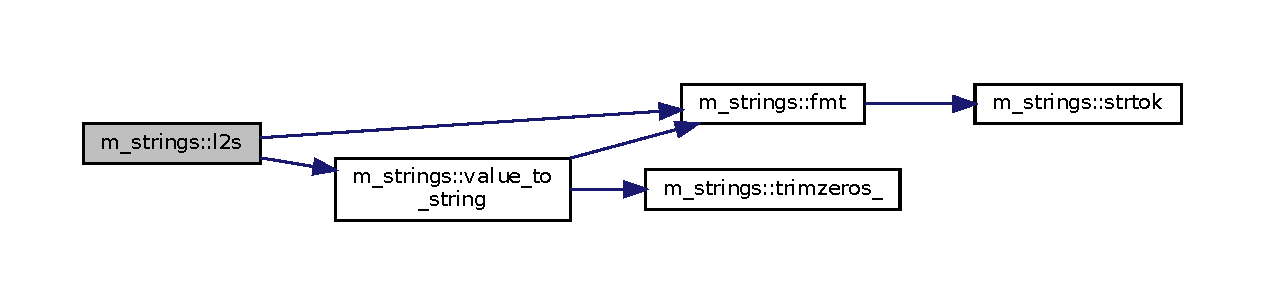
\includegraphics[width=350pt]{namespacem__strings_a75aa4dfd0a231e2bcad03d26231a7c29_cgraph}
\end{center}
\end{figure}
\mbox{\Hypertarget{namespacem__strings_aa1427d5dd673ff986236ba1732e693c1}\label{namespacem__strings_aa1427d5dd673ff986236ba1732e693c1}} 
\index{m\+\_\+strings@{m\+\_\+strings}!len\+\_\+white@{len\+\_\+white}}
\index{len\+\_\+white@{len\+\_\+white}!m\+\_\+strings@{m\+\_\+strings}}
\subsubsection{\texorpdfstring{len\+\_\+white()}{len\_white()}}
{\footnotesize\ttfamily elemental integer function, public m\+\_\+strings\+::len\+\_\+white (\begin{DoxyParamCaption}\item[{character(len=$\ast$), intent(in)}]{string }\end{DoxyParamCaption})}



\subsubsection*{N\+A\+ME}

len\+\_\+white(3f) -\/ \mbox{[}M\+\_\+strings\+:L\+E\+N\+G\+TH\mbox{]} get length of string trimmed of whitespace. (L\+I\+C\+E\+N\+SE\+:PD) 

\subsubsection*{S\+Y\+N\+O\+P\+S\+IS}

\begin{DoxyVerb}integer function len_white(string)

 character(len=*) :: string
\end{DoxyVerb}
 \subsubsection*{D\+E\+S\+C\+R\+I\+P\+T\+I\+ON}

len\+\_\+white(3f) returns the position of the last character in string that is not a whitespace character. The Fortran90 intrinsic L\+E\+N\+\_\+\+T\+R\+I\+M() should be used when trailing whitespace can be assumed to always be spaces.

This procedure was heavily used in the past because A\+N\+SI F\+O\+R\+T\+R\+AN 77 character objects are fixed length and blank padded and the L\+E\+N\+\_\+\+T\+R\+I\+M() intrinsic did not exist. It should now be used only when whitespace characters other than blanks are likely. \subsubsection*{O\+P\+T\+I\+O\+NS}

string input string whose trimmed length is being calculated ignoring all trailing whitespace characters. \subsubsection*{R\+E\+T\+U\+R\+NS}

len\+\_\+white the number of characters in the trimmed string

\subsubsection*{E\+X\+A\+M\+P\+LE}

Sample Program\+: \begin{DoxyVerb}program demo_len_white

use M_strings, only : len_white
character(len=80) ::  s
intrinsic len

  s=' ABCDEFG abcdefg '
  ilen = len(s)
  lastnb = len_white(s)

  write(*,*) 'total length of variable is ',ilen
  write(*,*) 'trimmed length of variable is ',lastnb
  write(*,*) 'trimmed string=[',s(:lastnb),']'

 end program demo_len_white
\end{DoxyVerb}


\subsubsection*{N\+O\+T\+ES}

o len\+\_\+white \begin{DoxyVerb} is a resource-intensive routine. Once the end of
 the string is found, it is probably best to keep track of it in
 order to avoid repeated calls to len_white. Because they
 might be more efficient, consider looking for vendor-supplied or
 system-optimized equivalents. For example:

    o lnblnk - Solaris f77
    o len_trim - FORTRAN 90
\end{DoxyVerb}


o Some compilers seem to have trouble passing a string of variable length properly. To be safe, use something like this\+: \begin{DoxyVerb}subroutine message(s)
 character(len=*) :: s ! s is of variable length
    ilen=len(s)        ! get total length of variable
    ! explicitly specify a substring instead of just variable name
    lastnb = len_white(s(:ilen))
    write(*,*)'error:[',s(:lastnb),']'
end subroutine messages
\end{DoxyVerb}


\subsubsection*{A\+U\+T\+H\+OR}

John S. Urban \subsubsection*{L\+I\+C\+E\+N\+SE}

Public Domain \mbox{\Hypertarget{namespacem__strings_a378563bb49f128bf0cf9c9d2b1f34498}\label{namespacem__strings_a378563bb49f128bf0cf9c9d2b1f34498}} 
\index{m\+\_\+strings@{m\+\_\+strings}!lenset@{lenset}}
\index{lenset@{lenset}!m\+\_\+strings@{m\+\_\+strings}}
\subsubsection{\texorpdfstring{lenset()}{lenset()}}
{\footnotesize\ttfamily character(len=length) function, public m\+\_\+strings\+::lenset (\begin{DoxyParamCaption}\item[{character(len=$\ast$), intent(in)}]{line,  }\item[{integer, intent(in)}]{length }\end{DoxyParamCaption})}



\subsubsection*{N\+A\+ME}

lenset(3f) -\/ \mbox{[}M\+\_\+strings\+:L\+E\+N\+G\+TH\mbox{]} return string trimmed or padded to specified length (L\+I\+C\+E\+N\+SE\+:PD) 

\subsubsection*{S\+Y\+N\+O\+P\+S\+IS}

\begin{DoxyVerb}function lenset(str,length) result(strout)

 character(len=*)                     :: str
 character(len=length)                :: strout
 integer,intent(in)                   :: length
\end{DoxyVerb}
 \subsubsection*{D\+E\+S\+C\+R\+I\+P\+T\+I\+ON}

lenset(3f) truncates a string or pads it with spaces to the specified length. \subsubsection*{O\+P\+T\+I\+O\+NS}

str input string length output string length \subsubsection*{R\+E\+S\+U\+L\+TS}

strout output string \subsubsection*{E\+X\+A\+M\+P\+LE}

Sample Program\+: \begin{DoxyVerb} program demo_lenset
  use M_strings, only : lenset
  implicit none
  character(len=10)            :: string='abcdefghij'
  character(len=:),allocatable :: answer
     answer=lenset(string,5)
     write(*,'("[",a,"]")') answer
     answer=lenset(string,20)
     write(*,'("[",a,"]")') answer
 end program demo_lenset
\end{DoxyVerb}


Expected output\+: \begin{DoxyVerb}[abcde]
[abcdefghij          ]
\end{DoxyVerb}


\subsubsection*{A\+U\+T\+H\+OR}

John S. Urban \subsubsection*{L\+I\+C\+E\+N\+SE}

Public Domain Here is the caller graph for this function\+:
\nopagebreak
\begin{figure}[H]
\begin{center}
\leavevmode
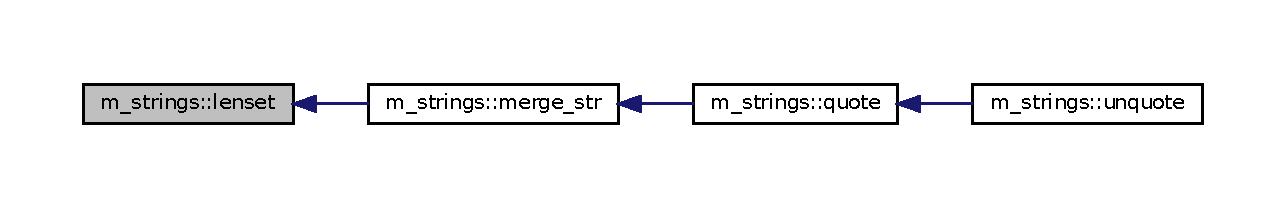
\includegraphics[width=350pt]{namespacem__strings_a378563bb49f128bf0cf9c9d2b1f34498_icgraph}
\end{center}
\end{figure}
\mbox{\Hypertarget{namespacem__strings_a81b4b7f4f301b9e17604adbcace58d0c}\label{namespacem__strings_a81b4b7f4f301b9e17604adbcace58d0c}} 
\index{m\+\_\+strings@{m\+\_\+strings}!listout@{listout}}
\index{listout@{listout}!m\+\_\+strings@{m\+\_\+strings}}
\subsubsection{\texorpdfstring{listout()}{listout()}}
{\footnotesize\ttfamily subroutine, public m\+\_\+strings\+::listout (\begin{DoxyParamCaption}\item[{integer, dimension(\+:), intent(in)}]{icurve\+\_\+lists,  }\item[{integer, dimension(\+:), intent(out)}]{icurve\+\_\+expanded,  }\item[{integer, intent(out)}]{inums\+\_\+out,  }\item[{integer, intent(out)}]{ierr }\end{DoxyParamCaption})}



\subsubsection*{N\+A\+ME}

listout(3f) -\/ \mbox{[}M\+\_\+strings\+:N\+U\+M\+E\+R\+IC\mbox{]} expand a list of numbers where negative numbers denote range ends (1 -\/10 means 1 thru 10) (L\+I\+C\+E\+N\+SE\+:PD) 

\subsubsection*{S\+Y\+N\+O\+P\+S\+IS}

subroutine listout(icurve\+\_\+lists,icurve\+\_\+expanded,inums,ierr)

integer,intent(in) \+:\+: icurve\+\_\+lists(\+:) integer,intent(out) \+:\+: icurve\+\_\+expanded(\+:) integer,intent(out) \+:\+: inums integer,intent(out) \+:\+: ierr \subsubsection*{D\+E\+S\+C\+R\+I\+P\+T\+I\+ON}

\subsubsection*{O\+P\+T\+I\+O\+NS}

icurve\+\_\+lists(\+:) input array

\subsubsection*{R\+E\+T\+U\+R\+NS}

icurve\+\_\+expanded(\+:) output array; assumed large enough to hold returned list inums number of icurve\+\_\+expanded numbers on output ierr zero if no error occurred

\subsubsection*{E\+X\+A\+M\+P\+LE}

Sample program\+: \begin{DoxyVerb} program demo_listout
 use M_strings, only : listout
 implicit none
 integer,allocatable :: icurve_lists(:)
 integer :: icurve_expanded(1000)
 ! icurve_lists is input array
 integer :: inums
 ! icurve_expanded is output array
 integer :: i
 ! number of icurve_lists values on input, number of icurve_expanded numbers on output
 integer :: ierr
    icurve_lists=[1, 20, -30, 101, 100, 99, 100, -120, 222, -200]
    inums=size(icurve_lists)
    call listout(icurve_lists,icurve_expanded,inums,ierr)
    if(ierr.eq.0)then
       write(*,'(i0)')(icurve_expanded(i),i=1,inums)
    else
       write(*,'(a,i0)')'error occurred in *listout* ',ierr
       write(*,'(i0)')(icurve_expanded(i),i=1,inums)
    endif
 end program demo_listout
\end{DoxyVerb}


\subsubsection*{A\+U\+T\+H\+OR}

John S. Urban \subsubsection*{L\+I\+C\+E\+N\+SE}

Public Domain \mbox{\Hypertarget{namespacem__strings_a3c7d4be9051206e4b2f72112f9fdc3b4}\label{namespacem__strings_a3c7d4be9051206e4b2f72112f9fdc3b4}} 
\index{m\+\_\+strings@{m\+\_\+strings}!lower@{lower}}
\index{lower@{lower}!m\+\_\+strings@{m\+\_\+strings}}
\subsubsection{\texorpdfstring{lower()}{lower()}}
{\footnotesize\ttfamily elemental pure character(len(str)) function, public m\+\_\+strings\+::lower (\begin{DoxyParamCaption}\item[{character($\ast$), intent(in)}]{str,  }\item[{integer, intent(in), optional}]{begin,  }\item[{integer, intent(in), optional}]{end }\end{DoxyParamCaption})}



\subsubsection*{N\+A\+ME}

lower(3f) -\/ \mbox{[}M\+\_\+strings\+:C\+A\+SE\mbox{]} changes a string to lowercase over specified range (L\+I\+C\+E\+N\+SE\+:PD) 

\subsubsection*{S\+Y\+N\+O\+P\+S\+IS}

\begin{DoxyVerb}elemental pure function lower(str,begin,end) result (string)

 character(*), intent(in) :: str
 integer,optional         :: begin, end
 character(len(str))      :: string  ! output string
\end{DoxyVerb}
 \subsubsection*{D\+E\+S\+C\+R\+I\+P\+T\+I\+ON}

lower(string) returns a copy of the input string with all characters converted to miniscule over the specified range, assuming A\+S\+C\+II character sets are being used. If no range is specified the entire string is converted to miniscule.

\subsubsection*{O\+P\+T\+I\+O\+NS}

str string to convert to miniscule begin optional starting position in \char`\"{}str\char`\"{} to begin converting to miniscule end optional ending position in \char`\"{}str\char`\"{} to stop converting to miniscule

\subsubsection*{R\+E\+S\+U\+L\+TS}

lower copy of the input string with all characters converted to miniscule over optionally specified range.

\subsubsection*{T\+R\+I\+V\+IA}

The terms \char`\"{}uppercase\char`\"{} and \char`\"{}lowercase\char`\"{} date back to the early days of the mechanical printing press. Individual metal alloy casts of each needed letter, or punctuation symbol, were meticulously added to a press block, by hand, before rolling out copies of a page. These metal casts were stored and organized in wooden cases. The more often needed miniscule letters were placed closer to hand, in the lower cases of the work bench. The less often needed, capitalized, majuscule letters, ended up in the harder to reach upper cases.

\subsubsection*{E\+X\+A\+M\+P\+LE}

Sample program\+: \begin{DoxyVerb}program demo_lower
use M_strings, only: lower
implicit none
character(len=:),allocatable  :: s
   s=' ABCDEFG abcdefg '
   write(*,*) 'mixed-case input string is ....',s
   write(*,*) 'lower-case output string is ...',lower(s)
end program demo_lower
\end{DoxyVerb}


Expected output \begin{DoxyVerb}mixed-case input string is .... ABCDEFG abcdefg
lower-case output string is ... abcdefg abcdefg
\end{DoxyVerb}
 \subsubsection*{A\+U\+T\+H\+OR}

John S. Urban \subsubsection*{L\+I\+C\+E\+N\+SE}

Public Domain Here is the caller graph for this function\+:
\nopagebreak
\begin{figure}[H]
\begin{center}
\leavevmode
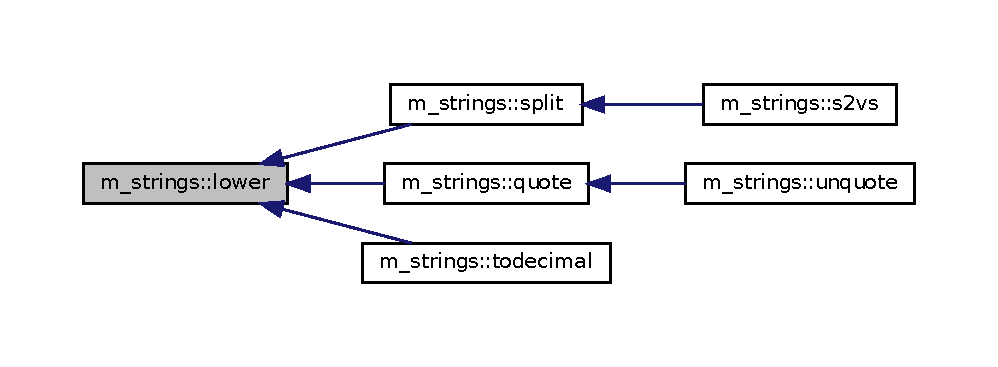
\includegraphics[width=350pt]{namespacem__strings_a3c7d4be9051206e4b2f72112f9fdc3b4_icgraph}
\end{center}
\end{figure}
\mbox{\Hypertarget{namespacem__strings_a5f96f66162f0f04d58b4f5dced8e82c6}\label{namespacem__strings_a5f96f66162f0f04d58b4f5dced8e82c6}} 
\index{m\+\_\+strings@{m\+\_\+strings}!matchw@{matchw}}
\index{matchw@{matchw}!m\+\_\+strings@{m\+\_\+strings}}
\subsubsection{\texorpdfstring{matchw()}{matchw()}}
{\footnotesize\ttfamily logical function, public m\+\_\+strings\+::matchw (\begin{DoxyParamCaption}\item[{character(len=$\ast$)}]{tame,  }\item[{character(len=$\ast$)}]{wild }\end{DoxyParamCaption})}



\subsubsection*{N\+A\+ME}

matchw(3f) -\/ \mbox{[}M\+\_\+strings\+:C\+O\+M\+P\+A\+RE\mbox{]} compare given string for match to pattern which may contain wildcard characters (L\+I\+C\+E\+N\+SE\+:PD) 

\subsubsection*{S\+Y\+N\+O\+P\+S\+IS}

\begin{DoxyVerb}logical function matchw(string, pattern )

 character(len=*),intent(in) :: string
 character(len=*),intent(in) :: pattern
\end{DoxyVerb}
 \subsubsection*{D\+E\+S\+C\+R\+I\+P\+T\+I\+ON}

\begin{DoxyVerb}matchw(3f) compares given STRING for match to PATTERN which may
contain wildcard characters.

In this version to get a match the entire string must be described
by PATTERN. Trailing whitespace is significant, so trim the input
string to have trailing whitespace ignored.
\end{DoxyVerb}


\subsubsection*{O\+P\+T\+I\+O\+NS}

string the input string to test to see if it contains the pattern. pattern the following simple globbing options are available o \char`\"{}?\char`\"{} matching any one character o \char`\"{}$\ast$\char`\"{} matching zero or more characters. Do N\+OT use adjacent asterisks. o Both strings may have trailing spaces which are ignored. o There is no escape character, so matching strings with literal question mark and asterisk is problematic.

\subsubsection*{E\+X\+A\+M\+P\+L\+ES}

Example program \begin{DoxyVerb}program demo_matchw
implicit none
! This main() routine passes a bunch of test strings into the above code.
! In performance comparison mode, it does that over and over. Otherwise,
! it does it just once. Either way, it outputs a passed/failed result.
!
integer :: nReps
logical :: allpassed
integer :: i
 allpassed = .true.

 nReps = 10000
 nReps = 1     ! Can choose as many repetitions as you're expecting in the real world.

 do i=1,nReps
  ! Cases with repeating character sequences.
  allpassed=allpassed .and. test("a*abab", "a*b", .true.)
  ! cycle
  allpassed=allpassed .and. test("ab", "*?", .true.)
  allpassed=allpassed .and. test("abc", "*?", .true.)
  allpassed=allpassed .and. test("abcccd", "*ccd", .true.)
  allpassed=allpassed .and. test("bLah", "bLaH", .false.)
  allpassed=allpassed .and. test("mississippi", "*sip*", .true.)
  allpassed=allpassed .and. test("xxxx*zzzzzzzzy*f", "xxx*zzy*f", .true.)
  allpassed=allpassed .and. test("xxxx*zzzzzzzzy*f", "xxxx*zzy*fffff", .false.)
  allpassed=allpassed .and. test("mississipissippi", "*issip*ss*", .true.)
  allpassed=allpassed .and. test("xxxxzzzzzzzzyf", "xxxx*zzy*fffff", .false.)
  allpassed=allpassed .and. test("xxxxzzzzzzzzyf", "xxxx*zzy*f", .true.)
  allpassed=allpassed .and. test("xyxyxyzyxyz", "xy*z*xyz", .true.)
  allpassed=allpassed .and. test("xyxyxyxyz", "xy*xyz", .true.)
  allpassed=allpassed .and. test("mississippi", "mi*sip*", .true.)
  allpassed=allpassed .and. test("ababac", "*abac*", .true.)
  allpassed=allpassed .and. test("aaazz", "a*zz*", .true.)
  allpassed=allpassed .and. test("a12b12", "*12*23", .false.)
  allpassed=allpassed .and. test("a12b12", "a12b", .false.)
  allpassed=allpassed .and. test("a12b12", "*12*12*", .true.)

  ! Additional cases where the '*' char appears in the tame string.
  allpassed=allpassed .and. test("*", "*", .true.)
  allpassed=allpassed .and. test("a*r", "a*", .true.)
  allpassed=allpassed .and. test("a*ar", "a*aar", .false.)

  ! More double wildcard scenarios.
  allpassed=allpassed .and. test("XYXYXYZYXYz", "XY*Z*XYz", .true.)
  allpassed=allpassed .and. test("missisSIPpi", "*SIP*", .true.)
  allpassed=allpassed .and. test("mississipPI", "*issip*PI", .true.)
  allpassed=allpassed .and. test("xyxyxyxyz", "xy*xyz", .true.)
  allpassed=allpassed .and. test("miSsissippi", "mi*sip*", .true.)
  allpassed=allpassed .and. test("miSsissippi", "mi*Sip*", .false.)
  allpassed=allpassed .and. test("abAbac", "*Abac*", .true.)
  allpassed=allpassed .and. test("aAazz", "a*zz*", .true.)
  allpassed=allpassed .and. test("A12b12", "*12*23", .false.)
  allpassed=allpassed .and. test("a12B12", "*12*12*", .true.)
  allpassed=allpassed .and. test("oWn", "*oWn*", .true.)

  ! Completely tame (no wildcards) cases.
  allpassed=allpassed .and. test("bLah", "bLah", .true.)

  ! Simple mixed wildcard tests suggested by IBMer Marlin Deckert.
  allpassed=allpassed .and. test("a", "*?", .true.)

  ! More mixed wildcard tests including coverage for false positives.
  allpassed=allpassed .and. test("a", "??", .false.)
  allpassed=allpassed .and. test("ab", "?*?", .true.)
  allpassed=allpassed .and. test("ab", "*?*?*", .true.)
  allpassed=allpassed .and. test("abc", "?**?*?", .true.)
  allpassed=allpassed .and. test("abc", "?**?*&?", .false.)
  allpassed=allpassed .and. test("abcd", "?b*??", .true.)
  allpassed=allpassed .and. test("abcd", "?a*??", .false.)
  allpassed=allpassed .and. test("abcd", "?**?c?", .true.)
  allpassed=allpassed .and. test("abcd", "?**?d?", .false.)
  allpassed=allpassed .and. test("abcde", "?*b*?*d*?", .true.)

  ! Single-character-match cases.
  allpassed=allpassed .and. test("bLah", "bL?h", .true.)
  allpassed=allpassed .and. test("bLaaa", "bLa?", .false.)
  allpassed=allpassed .and. test("bLah", "bLa?", .true.)
  allpassed=allpassed .and. test("bLaH", "?Lah", .false.)
  allpassed=allpassed .and. test("bLaH", "?LaH", .true.)

  ! Many-wildcard scenarios.
  allpassed=allpassed .and. test(&
  &"aaaaaaaaaaaaaaaaaaaaaaaaaaaaaaaaaaaaaaaaaaaaaaaaaaaaaaaaaaaaaaaaaaaaaaaaaaaaaaaaaaaaaaaaaab",&
  &"a*a*a*a*a*a*aa*aaa*a*a*b",&
  &.true.)
  allpassed=allpassed .and. test(&
  &"abababababababababababababababababababaacacacacacacacadaeafagahaiajakalaaaaaaaaaaaaaaaaaffafagaagggagaaaaaaaab",&
  &"*a*b*ba*ca*a*aa*aaa*fa*ga*b*",&
  &.true.)
  allpassed=allpassed .and. test(&
  &"abababababababababababababababababababaacacacacacacacadaeafagahaiajakalaaaaaaaaaaaaaaaaaffafagaagggagaaaaaaaab",&
  &"*a*b*ba*ca*a*x*aaa*fa*ga*b*",&
  &.false.)
  allpassed=allpassed .and. test(&
  &"abababababababababababababababababababaacacacacacacacadaeafagahaiajakalaaaaaaaaaaaaaaaaaffafagaagggagaaaaaaaab",&
  &"*a*b*ba*ca*aaaa*fa*ga*gggg*b*",&
  &.false.)
  allpassed=allpassed .and. test(&
  &"abababababababababababababababababababaacacacacacacacadaeafagahaiajakalaaaaaaaaaaaaaaaaaffafagaagggagaaaaaaaab",&
  &"*a*b*ba*ca*aaaa*fa*ga*ggg*b*",&
  &.true.)
  allpassed=allpassed .and. test("aaabbaabbaab", "*aabbaa*a*", .true.)
  allpassed=allpassed .and. test("a*a*a*a*a*a*a*a*a*a*a*a*a*a*a*a*a*", "a*a*a*a*a*a*a*a*a*a*a*a*a*a*a*a*a*", .true.)
  allpassed=allpassed .and. test("aaaaaaaaaaaaaaaaa", "*a*a*a*a*a*a*a*a*a*a*a*a*a*a*a*a*a*", .true.)
  allpassed=allpassed .and. test("aaaaaaaaaaaaaaaa", "*a*a*a*a*a*a*a*a*a*a*a*a*a*a*a*a*a*", .false.)
  allpassed=allpassed .and. test(&
  &"abc*abcd*abcde*abcdef*abcdefg*abcdefgh*abcdefghi*abcdefghij*abcdefghijk*abcdefghijkl*abcdefghijklm*abcdefghijklmn",&
  & "abc*abc*abc*abc*abc*abc*abc*abc*abc*abc*abc*abc*abc*abc*abc*abc*abc*",&
  &.false.)
  allpassed=allpassed .and. test(&
  &"abc*abcd*abcde*abcdef*abcdefg*abcdefgh*abcdefghi*abcdefghij*abcdefghijk*abcdefghijkl*abcdefghijklm*abcdefghijklmn",&
  &"abc*abc*abc*abc*abc*abc*abc*abc*abc*abc*abc*abc*",&
  &.true.)
  allpassed=allpassed .and. test("abc*abcd*abcd*abc*abcd", "abc*abc*abc*abc*abc", .false.)
  allpassed=allpassed .and. test( "abc*abcd*abcd*abc*abcd*abcd*abc*abcd*abc*abc*abcd", &
  &"abc*abc*abc*abc*abc*abc*abc*abc*abc*abc*abcd",&
  &.true.)
  allpassed=allpassed .and. test("abc", "********a********b********c********", .true.)
  allpassed=allpassed .and. test("********a********b********c********", "abc", .false.)
  allpassed=allpassed .and. test("abc", "********a********b********b********", .false.)
  allpassed=allpassed .and. test("*abc*", "***a*b*c***", .true.)

  ! A case-insensitive algorithm test.
  ! allpassed=allpassed .and. test("mississippi", "*issip*PI", .true.)
 enddo

 if (allpassed)then
    write(*,'(a)')"Passed",nReps
 else
    write(*,'(a)')"Failed"
 endif
contains
! This is a test program for wildcard matching routines. It can be used
! either to test a single routine for correctness, or to compare the timings
! of two (or more) different wildcard matching routines.
!
function test(tame, wild, bExpectedResult) result(bpassed)
use M_strings, only : matchw
   character(len=*) :: tame
   character(len=*) :: wild
   logical          :: bExpectedResult
   logical          :: bResult
   logical          :: bPassed
   bResult = .true.    ! We'll do "&=" cumulative checking.
   bPassed = .false.   ! Assume the worst.
   write(*,*)repeat('=',79)
   bResult = matchw(tame, wild) ! Call a wildcard matching routine.

   ! To assist correctness checking, output the two strings in any failing scenarios.
   if (bExpectedResult .eqv. bResult) then
      bPassed = .true.
      if(nReps == 1) write(*,*)"Passed match on ",tame," vs. ", wild
   else
      if(nReps == 1) write(*,*)"Failed match on ",tame," vs. ", wild
   endif

end function test
end program demo_matchw
\end{DoxyVerb}


Expected output

\subsubsection*{A\+U\+T\+H\+OR}

John S. Urban

\subsubsection*{R\+E\+F\+E\+R\+E\+N\+CE}

The article \char`\"{}\+Matching Wildcards\+: An Empirical Way to Tame an Algorithm\char`\"{} in Dr Dobb\textquotesingle{}s Journal, By Kirk J. Krauss, October 07, 2014

\subsubsection*{L\+I\+C\+E\+N\+SE}

Public Domain Here is the caller graph for this function\+:
\nopagebreak
\begin{figure}[H]
\begin{center}
\leavevmode
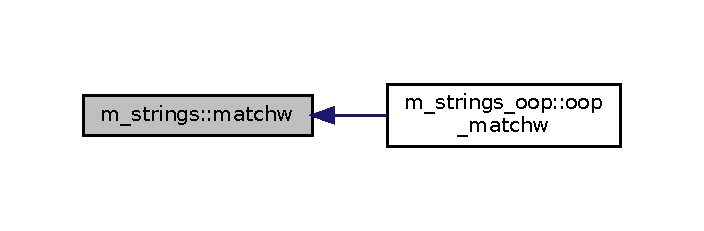
\includegraphics[width=338pt]{namespacem__strings_a5f96f66162f0f04d58b4f5dced8e82c6_icgraph}
\end{center}
\end{figure}
\mbox{\Hypertarget{namespacem__strings_aba5a8d7fc092b38d1939f37a13247c1e}\label{namespacem__strings_aba5a8d7fc092b38d1939f37a13247c1e}} 
\index{m\+\_\+strings@{m\+\_\+strings}!merge\+\_\+str@{merge\+\_\+str}}
\index{merge\+\_\+str@{merge\+\_\+str}!m\+\_\+strings@{m\+\_\+strings}}
\subsubsection{\texorpdfstring{merge\+\_\+str()}{merge\_str()}}
{\footnotesize\ttfamily character(len=\+:) function, allocatable, public m\+\_\+strings\+::merge\+\_\+str (\begin{DoxyParamCaption}\item[{character(len=$\ast$), intent(in), optional}]{str1,  }\item[{character(len=$\ast$), intent(in), optional}]{str2,  }\item[{logical, intent(in)}]{expr }\end{DoxyParamCaption})}



\subsubsection*{N\+A\+ME}

merge\+\_\+str(3f) -\/ \mbox{[}M\+\_\+strings\+:L\+E\+N\+G\+TH\mbox{]} pads strings to same length and then calls M\+E\+R\+G\+E(3f) (L\+I\+C\+E\+N\+SE\+:PD) 

\subsubsection*{S\+Y\+N\+O\+P\+S\+IS}

\begin{DoxyVerb}function merge_str(str1,str2,expr) result(strout)

 character(len=*),intent(in),optional :: str1
 character(len=*),intent(in),optional :: str2
 logical,intent(in)              :: expr
 character(len=:),allocatable    :: strout
\end{DoxyVerb}
 \subsubsection*{D\+E\+S\+C\+R\+I\+P\+T\+I\+ON}

merge\+\_\+str(3f) pads the shorter of str1 and str2 to the longest length of str1 and str2 and then calls M\+E\+R\+G\+E(padded\+\_\+str1,padded\+\_\+str2,expr). It trims trailing spaces off the result and returns the trimmed string. This makes it easier to call M\+E\+R\+G\+E(3f) with strings, as M\+E\+R\+G\+E(3f) requires the strings to be the same length.

N\+O\+TE\+: S\+T\+R1 and S\+T\+R2 are always required even though declared optional. this is so the call \char`\"{}\+S\+T\+R\+\_\+\+M\+E\+R\+G\+E(\+A,\+B,present(\+A))\char`\"{} is a valid call. The parameters S\+T\+R1 and S\+T\+R2 when they are optional parameters can be passed to a procedure if the options are optional on the called procedure.

\subsubsection*{O\+P\+T\+I\+O\+NS}

S\+T\+R1 string to return if the logical expression E\+X\+PR is true S\+T\+R2 string to return if the logical expression E\+X\+PR is false E\+X\+PR logical expression to evaluate to determine whether to return S\+T\+R1 when true, and S\+T\+R2 when false. \subsubsection*{R\+E\+S\+U\+LT}

M\+E\+R\+G\+E\+\_\+\+S\+TR a trimmed string is returned that is otherwise the value of S\+T\+R1 or S\+T\+R2, depending on the logical expression E\+X\+PR.

\subsubsection*{E\+X\+A\+M\+P\+L\+ES}

Sample Program\+: \begin{DoxyVerb} program demo_merge_str
 use M_strings, only : merge_str
 implicit none
 character(len=:), allocatable :: answer
    answer=merge_str('first string', 'second string is longer',10.eq.10)
    write(*,'("[",a,"]")') answer
    answer=merge_str('first string', 'second string is longer',10.ne.10)
    write(*,'("[",a,"]")') answer
 end program demo_merge_str
\end{DoxyVerb}


Expected output \begin{DoxyVerb}[first string]
[second string is longer]
\end{DoxyVerb}
 \subsubsection*{A\+U\+T\+H\+OR}

John S. Urban \subsubsection*{L\+I\+C\+E\+N\+SE}

Public Domain 

References lenset().

Here is the call graph for this function\+:
\nopagebreak
\begin{figure}[H]
\begin{center}
\leavevmode
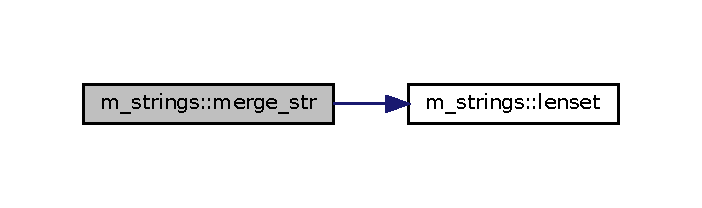
\includegraphics[width=337pt]{namespacem__strings_aba5a8d7fc092b38d1939f37a13247c1e_cgraph}
\end{center}
\end{figure}
Here is the caller graph for this function\+:
\nopagebreak
\begin{figure}[H]
\begin{center}
\leavevmode
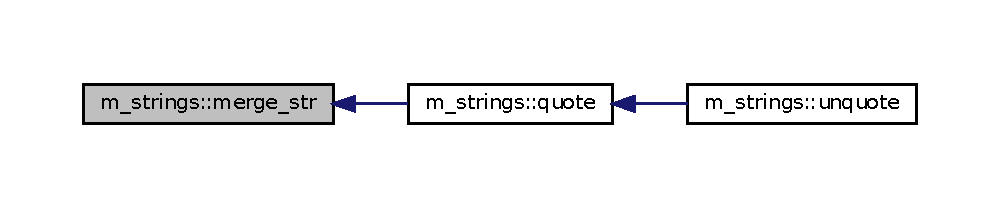
\includegraphics[width=350pt]{namespacem__strings_aba5a8d7fc092b38d1939f37a13247c1e_icgraph}
\end{center}
\end{figure}
\mbox{\Hypertarget{namespacem__strings_aec887410b018916a683fbb2ae529f8c5}\label{namespacem__strings_aec887410b018916a683fbb2ae529f8c5}} 
\index{m\+\_\+strings@{m\+\_\+strings}!modif@{modif}}
\index{modif@{modif}!m\+\_\+strings@{m\+\_\+strings}}
\subsubsection{\texorpdfstring{modif()}{modif()}}
{\footnotesize\ttfamily subroutine, public m\+\_\+strings\+::modif (\begin{DoxyParamCaption}\item[{character(len=$\ast$)}]{C\+L\+I\+NE,  }\item[{character(len=$\ast$), intent(in)}]{M\+OD }\end{DoxyParamCaption})}



\subsubsection*{N\+A\+ME}

modif(3f) -\/ \mbox{[}M\+\_\+strings\+:E\+D\+I\+T\+I\+NG\mbox{]} emulate the M\+O\+D\+I\+FY command from the line editor X\+E\+D\+IT (L\+I\+C\+E\+N\+SE\+:PD) 

\subsubsection*{S\+Y\+N\+O\+P\+S\+IS}

\begin{DoxyVerb}subroutine modif(cline,cmod)

 character(len=*) :: cline ! input string to change
 character(len=*) :: cmod  ! directive provides directions on changing string
\end{DoxyVerb}
 \subsubsection*{D\+E\+S\+C\+R\+I\+P\+T\+I\+ON}

M\+O\+D\+I\+F(3f) Modifies the line currently pointed at using a directive that acts much like a line editor directive. Primarily used to create interactive utilities such as input history editors for interactive line-\/mode programs.

the modify directives are as follows-\/

D\+I\+R\+E\+C\+T\+I\+VE E\+X\+P\+L\+A\+N\+A\+T\+I\+ON

$^\wedge$\+S\+T\+R\+I\+NG\# Causes the string of characters between the $^\wedge$ and the next \# to be inserted before the characters pointed to by the $^\wedge$. an $^\wedge$ or \& within the string is treated as a regular character. If the closing \# is not specified, M\+O\+D\+I\+F(3f) inserts the remainder of the line as if a \# was specified after the last nonblank character.

There are two exceptions. the combination $^\wedge$\# causes a \# to be inserted before the character pointed to by the $^\wedge$, and an $^\wedge$ as the last character of the directives causes a blank to be inserted.

\subsection*{(When not the first \# after an $^\wedge$) causes the character}

above it to be deleted.

\& Replaces the character above it with a space.

(S\+P\+A\+CE) A space below a character leaves it unchanged.

Any other character replaces the character above it.

\subsubsection*{E\+X\+A\+M\+P\+L\+ES}

Example input/output\+:

T\+HE I\+N\+P\+UT L\+I\+NE........ 10 T\+H\+IS S\+T\+R\+I\+NG TO BE M\+O\+R\+T\+I\+FD T\+HE D\+I\+R\+E\+C\+T\+I\+V\+ES L\+I\+NE... $^\wedge$ IS T\+HE\# D\# $^\wedge$\+IE A\+L\+T\+E\+R\+ED I\+N\+P\+UT L\+I\+NE.... 10 T\+H\+IS IS T\+HE S\+T\+R\+I\+NG TO BE M\+O\+D\+I\+F\+I\+ED

Sample program\+: \begin{DoxyVerb}program demo_modif
use M_strings, only : modif
implicit none
character(len=256)           :: line
integer                      :: ios
integer                      :: count
integer                      :: COMMAND_LINE_LENGTH
character(len=:),allocatable :: COMMAND_LINE
   ! get command name length
   call get_command_argument(0,length=count)
   ! get command line length
   call get_command(length=COMMAND_LINE_LENGTH)
   ! allocate string big enough to hold command line
   allocate(character(len=COMMAND_LINE_LENGTH+200) :: COMMAND_LINE)
   ! get command line as a string
   call get_command(command=COMMAND_LINE)
   ! trim leading spaces just in case
   COMMAND_LINE=adjustl(COMMAND_LINE)
   ! remove command name
   COMMAND_LINE=adjustl(COMMAND_LINE(COUNT+2:))
   INFINITE: do
      read(*,'(a)',iostat=ios)line
      if(ios.ne.0)exit
      call modif(line,COMMAND_LINE)
      write(*,'(a)')trim(line)
   enddo INFINITE
end program demo_modif
\end{DoxyVerb}


\subsubsection*{A\+U\+T\+H\+OR}

John S. Urban \subsubsection*{L\+I\+C\+E\+N\+SE}

Public Domain \mbox{\Hypertarget{namespacem__strings_a52d27df9dcea52039c6feccb782ec4fd}\label{namespacem__strings_a52d27df9dcea52039c6feccb782ec4fd}} 
\index{m\+\_\+strings@{m\+\_\+strings}!msg\+\_\+one@{msg\+\_\+one}}
\index{msg\+\_\+one@{msg\+\_\+one}!m\+\_\+strings@{m\+\_\+strings}}
\subsubsection{\texorpdfstring{msg\+\_\+one()}{msg\_one()}}
{\footnotesize\ttfamily character(len=\+:) function, allocatable m\+\_\+strings\+::msg\+\_\+one (\begin{DoxyParamCaption}\item[{class($\ast$), dimension(\+:), intent(in)}]{generic1,  }\item[{class($\ast$), dimension(\+:), intent(in), optional}]{generic2,  }\item[{class($\ast$), dimension(\+:), intent(in), optional}]{generic3,  }\item[{class($\ast$), dimension(\+:), intent(in), optional}]{generic4,  }\item[{class($\ast$), dimension(\+:), intent(in), optional}]{generic5,  }\item[{class($\ast$), dimension(\+:), intent(in), optional}]{generic6,  }\item[{class($\ast$), dimension(\+:), intent(in), optional}]{generic7,  }\item[{class($\ast$), dimension(\+:), intent(in), optional}]{generic8,  }\item[{class($\ast$), dimension(\+:), intent(in), optional}]{generic9,  }\item[{logical, intent(in), optional}]{nospace }\end{DoxyParamCaption})\hspace{0.3cm}{\ttfamily [private]}}



References nospace(), and print\+\_\+generic().

Here is the call graph for this function\+:
\nopagebreak
\begin{figure}[H]
\begin{center}
\leavevmode
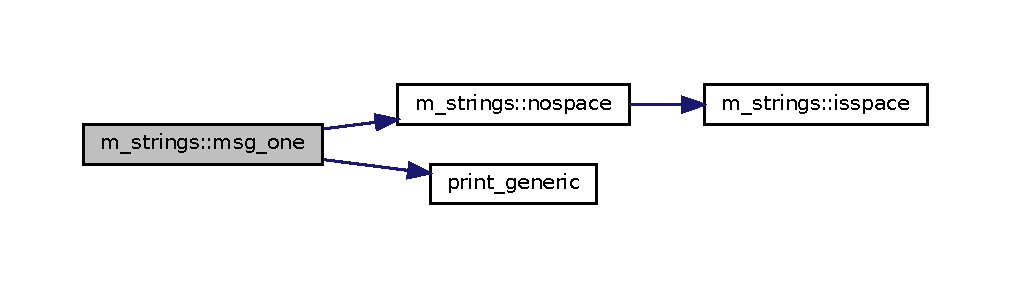
\includegraphics[width=350pt]{namespacem__strings_a52d27df9dcea52039c6feccb782ec4fd_cgraph}
\end{center}
\end{figure}
\mbox{\Hypertarget{namespacem__strings_a926d1d9f529487149f4e0a1de8294122}\label{namespacem__strings_a926d1d9f529487149f4e0a1de8294122}} 
\index{m\+\_\+strings@{m\+\_\+strings}!msg\+\_\+scalar@{msg\+\_\+scalar}}
\index{msg\+\_\+scalar@{msg\+\_\+scalar}!m\+\_\+strings@{m\+\_\+strings}}
\subsubsection{\texorpdfstring{msg\+\_\+scalar()}{msg\_scalar()}}
{\footnotesize\ttfamily character(len=\+:) function, allocatable m\+\_\+strings\+::msg\+\_\+scalar (\begin{DoxyParamCaption}\item[{class($\ast$), intent(in), optional}]{generic1,  }\item[{class($\ast$), intent(in), optional}]{generic2,  }\item[{class($\ast$), intent(in), optional}]{generic3,  }\item[{class($\ast$), intent(in), optional}]{generic4,  }\item[{class($\ast$), intent(in), optional}]{generic5,  }\item[{class($\ast$), intent(in), optional}]{generic6,  }\item[{class($\ast$), intent(in), optional}]{generic7,  }\item[{class($\ast$), intent(in), optional}]{generic8,  }\item[{class($\ast$), intent(in), optional}]{generic9,  }\item[{logical, intent(in), optional}]{nospace }\end{DoxyParamCaption})\hspace{0.3cm}{\ttfamily [private]}}



\subsubsection*{N\+A\+ME}

msg(3f) -\/ \mbox{[}M\+\_\+strings\mbox{]} converts any standard scalar type to a string (L\+I\+C\+E\+N\+SE\+:PD) \subsubsection*{S\+Y\+N\+O\+P\+S\+IS}

function msg(g1,g2g3,g4,g5,g6,g7,g8,g9,nospace)

class($\ast$),intent(in),optional \+:\+: g1,g2,g3,g4,g5,g6,g7,g8,g9 logical,intent(in),optional \+:\+: nospace character,len=(\+:),allocatable \+:\+: msg

\subsubsection*{D\+E\+S\+C\+R\+I\+P\+T\+I\+ON}

msg(3f) builds a space-\/separated string from up to nine scalar values.

\subsubsection*{O\+P\+T\+I\+O\+NS}

g\mbox{[}1-\/9\mbox{]} optional value to print the value of after the message. May be of type I\+N\+T\+E\+G\+ER, L\+O\+G\+I\+C\+AL, R\+E\+AL, D\+O\+U\+B\+L\+E\+P\+R\+E\+C\+I\+S\+I\+ON, C\+O\+M\+P\+L\+EX, or C\+H\+A\+R\+A\+C\+T\+ER. nospace if nospace=.true., then no spaces are added between values \subsubsection*{R\+E\+T\+U\+R\+NS}

msg description to print

\subsubsection*{E\+X\+A\+M\+P\+L\+ES}

Sample program\+: \begin{DoxyVerb} program demo_msg
 use M_strings, only : msg
 implicit none
 character(len=:),allocatable :: pr
 character(len=:),allocatable :: frmt
 integer                      :: biggest

 pr=msg('HUGE(3f) integers',huge(0),'and real',huge(0.0),'and double',huge(0.0d0))
 write(*,'(a)')pr
 pr=msg('real            :',huge(0.0),0.0,12345.6789,tiny(0.0) )
 write(*,'(a)')pr
 pr=msg('doubleprecision :',huge(0.0d0),0.0d0,12345.6789d0,tiny(0.0d0) )
 write(*,'(a)')pr
 pr=msg('complex         :',cmplx(huge(0.0),tiny(0.0)) )
 write(*,'(a)')pr

 ! create a format on the fly
 biggest=huge(0)
 frmt=msg('(*(i',int(log10(real(biggest))),':,1x))',nospace=.true.)
 write(*,*)'format=',frmt

 ! although it will often work, using msg(3f) in an I/O statement is not recommended
 write(*,*)msg('program will now stop')

 end program demo_msg
\end{DoxyVerb}


Output \begin{DoxyVerb}HUGE(3f) integers 2147483647 and real 3.40282347E+38 and double 1.7976931348623157E+308
real            : 3.40282347E+38 0.00000000 12345.6787 1.17549435E-38
doubleprecision : 1.7976931348623157E+308 0.0000000000000000 12345.678900000001 2.2250738585072014E-308
complex         : (3.40282347E+38,1.17549435E-38)
 format=(*(i9:,1x))
 program will now stop
\end{DoxyVerb}


\subsubsection*{A\+U\+T\+H\+OR}

John S. Urban \subsubsection*{L\+I\+C\+E\+N\+SE}

Public Domain 

References nospace(), and print\+\_\+generic().

Here is the call graph for this function\+:
\nopagebreak
\begin{figure}[H]
\begin{center}
\leavevmode
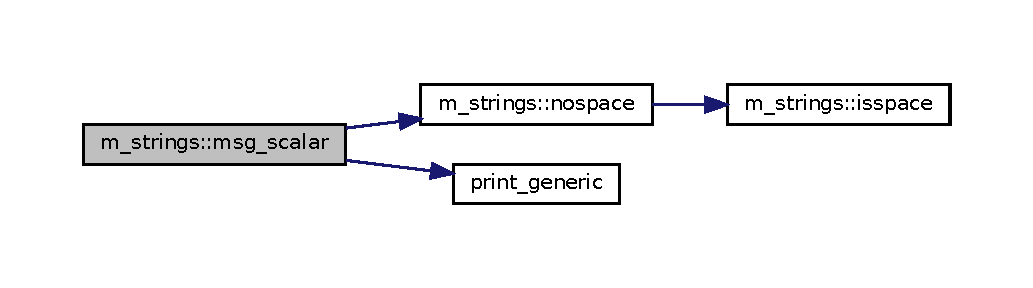
\includegraphics[width=350pt]{namespacem__strings_a926d1d9f529487149f4e0a1de8294122_cgraph}
\end{center}
\end{figure}
\mbox{\Hypertarget{namespacem__strings_a5d72fde097444c689f1822c5ad95e03d}\label{namespacem__strings_a5d72fde097444c689f1822c5ad95e03d}} 
\index{m\+\_\+strings@{m\+\_\+strings}!noesc@{noesc}}
\index{noesc@{noesc}!m\+\_\+strings@{m\+\_\+strings}}
\subsubsection{\texorpdfstring{noesc()}{noesc()}}
{\footnotesize\ttfamily elemental character(len=len(instr)) function, public m\+\_\+strings\+::noesc (\begin{DoxyParamCaption}\item[{character(len=$\ast$), intent(in)}]{I\+N\+S\+TR }\end{DoxyParamCaption})}



\subsubsection*{N\+A\+ME}

noesc(3f) -\/ \mbox{[}M\+\_\+strings\+:N\+O\+N\+A\+L\+P\+HA\mbox{]} convert non-\/printable characters to a space. (L\+I\+C\+E\+N\+SE\+:PD) 

\subsubsection*{S\+Y\+N\+O\+P\+S\+IS}

\begin{DoxyVerb}elemental function noesc(INSTR)

 character(len=*),intent(in) :: INSTR
 character(len=len(instr))   :: noesc
\end{DoxyVerb}
 \subsubsection*{D\+E\+S\+C\+R\+I\+P\+T\+I\+ON}

Convert non-\/printable characters to a space.

\subsubsection*{E\+X\+A\+M\+P\+L\+ES}

Sample Program\+: \begin{DoxyVerb}program demo_noesc

use M_strings, only : noesc
character(len=128) :: ascii
character(len=128) :: cleared
! fill variable with base ASCII character set
do i=1,128
   ascii(i:i)=char(i-1)
enddo
cleared=noesc(ascii)
write(*,*)'characters and their ADE (ASCII Decimal Equivalent)'
call ade(ascii)
write(*,*)'Cleared of non-printable characters'
call ade(cleared)
write(*,*)'Cleared string:'
write(*,*)cleared
contains
  subroutine ade(string)
  implicit none
  ! the string to print
  character(len=*),intent(in) :: string
  ! number of characters in string to print
  integer :: ilen
  ! counter used to step thru string
  integer :: i
     ! get trimmed length of input string
     ilen=len_trim(string(:len(string)))

     ! replace lower unprintable characters with spaces
     write(*,101)(merge(string(i:i),' ',&
     & ichar(string(i:i)).ge.32         &
     & .and.                            &
     & ichar(string(i:i)).le.126)       &
     & ,i=1,ilen)

     ! print ADE value of character underneath it
     write(*,202)     (ichar(string(i:i))/100,    i=1,ilen)
     write(*,202)(mod( ichar(string(i:i)),100)/10,i=1,ilen)
     write(*,202)(mod((ichar(string(i:i))),10),   i=1,ilen)
  ! format for printing string characters
  101   format(*(a1:))
  ! format for printing ADE values
  202   format(*(i1:))
  end subroutine ade
  end program demo_noesc
\end{DoxyVerb}


Expected output

The string is printed with the A\+DE value vertically beneath. The original string has all the A\+D\+Es from 000 to 127. After N\+O\+E\+S\+C(3f) is called on the string all the \char`\"{}non-\/printable\char`\"{} characters are replaced with a space (A\+DE of 032).

characters and their A\+DE (A\+S\+C\+II Decimal Equivalent)

$>$ !"\#\$\%\&\textquotesingle{}()$\ast$+,-\/./0123456789\+:;$<$=$>$?\mbox{[}\mbox{]}$^\wedge$\+\_\+\`{}abcdefghijklmnopqrstuvwxyz\{$\vert$\}$\sim$ $>$00000000000000000000000000000000000000000000000000000000000000000000000000000000000000000000000000001111111111111111111111111111 $>$00000000001111111111222222222233333333334444444444555555555566666666667777777777888888888899999999990000000000111111111122222222 $>$01234567890123456789012345678901234567890123456789012345678901234567890123456789012345678901234567890123456789012345678901234567

Cleared of non-\/printable characters

$>$ !"\#\$\%\&\textquotesingle{}()$\ast$+,-\/./0123456789\+:;$<$=$>$?\mbox{[}\mbox{]}$^\wedge$\+\_\+\`{}abcdefghijklmnopqrstuvwxyz\{$\vert$\}$\sim$ $>$0000000000000000000000000000000000000000000000000000000000000000000000000000000000000000000000000000111111111111111111111111111 $>$3333333333333333333333333333333333333333444444444455555555556666666666777777777788888888889999999999000000000011111111112222222 $>$2222222222222222222222222222222223456789012345678901234567890123456789012345678901234567890123456789012345678901234567890123456

Cleared string\+: $>$ !"\#\$\%\&\textquotesingle{}()$\ast$+,-\/./0123456789\+:;$<$=$>$?\mbox{[}\mbox{]}$^\wedge$\+\_\+\`{}abcdefghijklmnopqrstuvwxyz\{$\vert$\}$\sim$ \subsubsection*{A\+U\+T\+H\+OR}

John S. Urban \subsubsection*{L\+I\+C\+E\+N\+SE}

Public Domain \mbox{\Hypertarget{namespacem__strings_ad007f050abe3d142f4a7badbc4408685}\label{namespacem__strings_ad007f050abe3d142f4a7badbc4408685}} 
\index{m\+\_\+strings@{m\+\_\+strings}!nospace@{nospace}}
\index{nospace@{nospace}!m\+\_\+strings@{m\+\_\+strings}}
\subsubsection{\texorpdfstring{nospace()}{nospace()}}
{\footnotesize\ttfamily character(len=\+:) function, allocatable, public m\+\_\+strings\+::nospace (\begin{DoxyParamCaption}\item[{character(len=$\ast$), intent(in)}]{line }\end{DoxyParamCaption})}



\subsubsection*{N\+A\+ME}

nospace(3f) -\/ \mbox{[}M\+\_\+strings\+:W\+H\+I\+T\+E\+S\+P\+A\+CE\mbox{]} remove all whitespace from input string (L\+I\+C\+E\+N\+SE\+:PD) 

\subsubsection*{S\+Y\+N\+O\+P\+S\+IS}

\begin{DoxyVerb}function nospace(str) - remove all whitespace from input string

 character(len=*),intent(in)          :: str
 character(len=:),allocatable         :: nospace
\end{DoxyVerb}
 \subsubsection*{D\+E\+S\+C\+R\+I\+P\+T\+I\+ON}

\begin{DoxyVerb}nospace(3f) removes space, tab, carriage return, new line, vertical
tab, formfeed and null characters (called "whitespace"). The output
is returned trimmed.
\end{DoxyVerb}


\subsubsection*{E\+X\+A\+M\+P\+L\+ES}

Sample program\+: \begin{DoxyVerb} program demo_nospace
 use M_strings, only: nospace
 implicit none
 character(len=:),allocatable  :: s
    s='  This     is      a     test  '
    write(*,*) 'original input string is ....',s
    write(*,*) 'processed output string is ...',nospace(s)
    if(nospace(s).eq.'Thisisatest')then
       write(*,*)'nospace test passed'
    else
       write(*,*)'nospace test error'
    endif
 end program demo_nospace
\end{DoxyVerb}


Expected output \begin{DoxyVerb}original input string is ....  This     is      a     test
processed output string is ...Thisisatest
nospace test passed
\end{DoxyVerb}
 \subsubsection*{A\+U\+T\+H\+OR}

John S. Urban \subsubsection*{L\+I\+C\+E\+N\+SE}

Public Domain 

References isspace().

Here is the call graph for this function\+:
\nopagebreak
\begin{figure}[H]
\begin{center}
\leavevmode
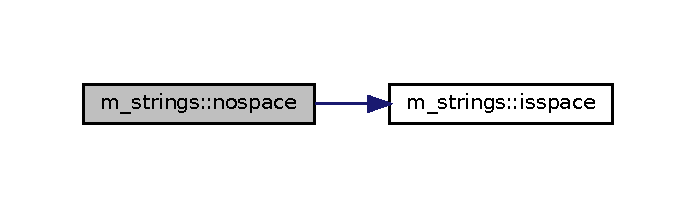
\includegraphics[width=334pt]{namespacem__strings_ad007f050abe3d142f4a7badbc4408685_cgraph}
\end{center}
\end{figure}
Here is the caller graph for this function\+:
\nopagebreak
\begin{figure}[H]
\begin{center}
\leavevmode
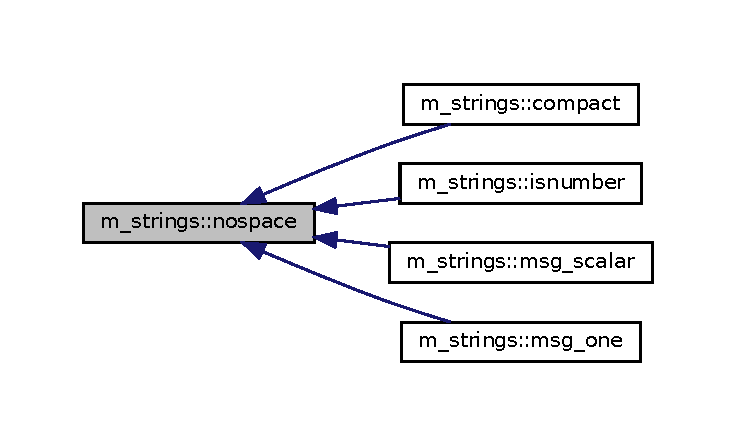
\includegraphics[width=350pt]{namespacem__strings_ad007f050abe3d142f4a7badbc4408685_icgraph}
\end{center}
\end{figure}
\mbox{\Hypertarget{namespacem__strings_a3bf44ac06a670f55830e17a6f1108b9c}\label{namespacem__strings_a3bf44ac06a670f55830e17a6f1108b9c}} 
\index{m\+\_\+strings@{m\+\_\+strings}!notabs@{notabs}}
\index{notabs@{notabs}!m\+\_\+strings@{m\+\_\+strings}}
\subsubsection{\texorpdfstring{notabs()}{notabs()}}
{\footnotesize\ttfamily subroutine, public m\+\_\+strings\+::notabs (\begin{DoxyParamCaption}\item[{character(len=$\ast$), intent(in)}]{I\+N\+S\+TR,  }\item[{character(len=$\ast$), intent(out)}]{O\+U\+T\+S\+TR,  }\item[{integer, intent(out)}]{I\+L\+EN }\end{DoxyParamCaption})}



\subsubsection*{N\+A\+ME}

notabs(3f) -\/ \mbox{[}M\+\_\+strings\+:N\+O\+N\+A\+L\+P\+HA\mbox{]} expand tab characters (L\+I\+C\+E\+N\+SE\+:PD) \subsubsection*{S\+Y\+N\+O\+P\+S\+IS}

subroutine notabs(\+I\+N\+S\+T\+R,\+O\+U\+T\+S\+T\+R,\+I\+L\+E\+N)

character(len=$\ast$),intent=(in) \+:\+: I\+N\+S\+TR character(len=$\ast$),intent=(out) \+:\+: O\+U\+T\+S\+TR integer,intent=(out) \+:\+: I\+L\+EN \subsubsection*{D\+E\+S\+C\+R\+I\+P\+T\+I\+ON}

N\+O\+T\+A\+B\+S() converts tabs in I\+N\+S\+TR to spaces in O\+U\+T\+S\+TR while maintaining columns. It assumes a tab is set every 8 characters. Trailing spaces are removed.

In addition, trailing carriage returns and line feeds are removed (they are usually a problem created by going to and from M\+S\+Windows).

What are some reasons for removing tab characters from an input line? Some Fortran compilers have problems with tabs, as tabs are not part of the Fortran character set. Some editors and printers will have problems with tabs. It is often useful to expand tabs in input files to simplify further processing such as tokenizing an input line.

\subsubsection*{O\+P\+T\+I\+O\+NS}

instr Input line to remove tabs from

\subsubsection*{R\+E\+S\+U\+L\+TS}

outstr Output string with tabs expanded. ilen Significant length of returned string

\subsubsection*{E\+X\+A\+M\+P\+L\+ES}

Sample program\+: \begin{DoxyVerb}program demo_notabs

!  test filter to remove tabs and trailing white space from input
!  on files up to 1024 characters wide
use M_strings, only : notabs
character(len=1024) :: in,out
integer             :: ios,iout
   READFILE: block
      do
         read(*,'(A)',iostat=ios)in
         if(ios /= 0) exit READFILE
         call notabs(in,out,iout)
         write(*,'(a)')out(:iout)
      enddo
   endblock READFILE

end program demo_notabs
\end{DoxyVerb}


\subsubsection*{S\+EE A\+L\+SO}

G\+N\+U/\+Unix commands expand(1) and unexpand(1)

\subsubsection*{A\+U\+T\+H\+OR}

John S. Urban \subsubsection*{L\+I\+C\+E\+N\+SE}

Public Domain \mbox{\Hypertarget{namespacem__strings_a3596a4ec755ac897a1dbc0b225d5266a}\label{namespacem__strings_a3596a4ec755ac897a1dbc0b225d5266a}} 
\index{m\+\_\+strings@{m\+\_\+strings}!quote@{quote}}
\index{quote@{quote}!m\+\_\+strings@{m\+\_\+strings}}
\subsubsection{\texorpdfstring{quote()}{quote()}}
{\footnotesize\ttfamily character(len=\+:) function, allocatable, public m\+\_\+strings\+::quote (\begin{DoxyParamCaption}\item[{character(len=$\ast$), intent(in)}]{str,  }\item[{character(len=$\ast$), intent(in), optional}]{mode,  }\item[{logical, intent(in), optional}]{clip }\end{DoxyParamCaption})}



\subsubsection*{N\+A\+ME}

quote(3f) -\/ \mbox{[}M\+\_\+strings\+:Q\+U\+O\+T\+ES\mbox{]} add quotes to string as if written with list-\/directed input (L\+I\+C\+E\+N\+SE\+:PD) \subsubsection*{S\+Y\+N\+O\+P\+S\+IS}

function quote(str,mode,clip) result (quoted\+\_\+str)

character(len=$\ast$),intent(in) \+:\+: str character(len=$\ast$),optional,intent(in) \+:\+: mode logical,optional,intent(in) \+:\+: clip character(len=\+:),allocatable \+:\+: quoted\+\_\+str \subsubsection*{D\+E\+S\+C\+R\+I\+P\+T\+I\+ON}

Add quotes to a C\+H\+A\+R\+A\+C\+T\+ER variable as if it was written using list-\/directed input. This is particularly useful for processing strings to add to C\+SV files.

\subsubsection*{O\+P\+T\+I\+O\+NS}

str input string to add quotes to, using the rules of list-\/directed input (single quotes are replaced by two adjacent quotes) mode alternate quoting methods are supported\+: \begin{DoxyVerb}           DOUBLE   default. replace quote with double quotes
           ESCAPE   replace quotes with backslash-quote instead of double quotes
\end{DoxyVerb}


clip default is to trim leading and trailing spaces from the string. If C\+L\+IP is .F\+A\+L\+SE. spaces are not trimmed

\subsubsection*{R\+E\+S\+U\+LT}

quoted\+\_\+str The output string, which is based on adding quotes to S\+TR. \subsubsection*{E\+X\+A\+M\+P\+LE}

Sample program\+: \begin{DoxyVerb}program demo_quote
use M_strings, only : quote
implicit none
character(len=:),allocatable :: str
character(len=1024)          :: msg
integer                      :: ios
character(len=80)            :: inline
   do
      write(*,'(a)',advance='no')'Enter test string:'
      read(*,'(a)',iostat=ios,iomsg=msg)inline
      if(ios.ne.0)then
         write(*,*)trim(inline)
         exit
      endif

      ! the original string
      write(*,'(a)')'ORIGINAL     ['//trim(inline)//']'

      ! the string processed by quote(3f)
      str=quote(inline)
      write(*,'(a)')'QUOTED     ['//str//']'

      ! write the string list-directed to compare the results
      write(*,'(a)',iostat=ios,iomsg=msg) 'LIST DIRECTED:'
      write(*,*,iostat=ios,iomsg=msg,delim='none') inline
      write(*,*,iostat=ios,iomsg=msg,delim='quote') inline
      write(*,*,iostat=ios,iomsg=msg,delim='apostrophe') inline
   enddo
end program demo_quote
\end{DoxyVerb}


\subsubsection*{A\+U\+T\+H\+OR}

John S. Urban \subsubsection*{L\+I\+C\+E\+N\+SE}

Public Domain 

References lower(), merge\+\_\+str(), and replace().

Here is the call graph for this function\+:
\nopagebreak
\begin{figure}[H]
\begin{center}
\leavevmode
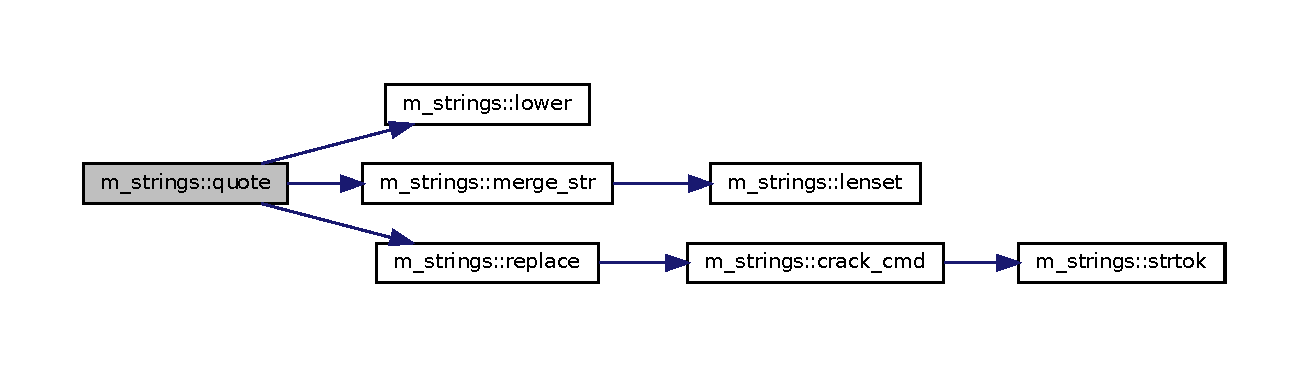
\includegraphics[width=350pt]{namespacem__strings_a3596a4ec755ac897a1dbc0b225d5266a_cgraph}
\end{center}
\end{figure}
Here is the caller graph for this function\+:
\nopagebreak
\begin{figure}[H]
\begin{center}
\leavevmode
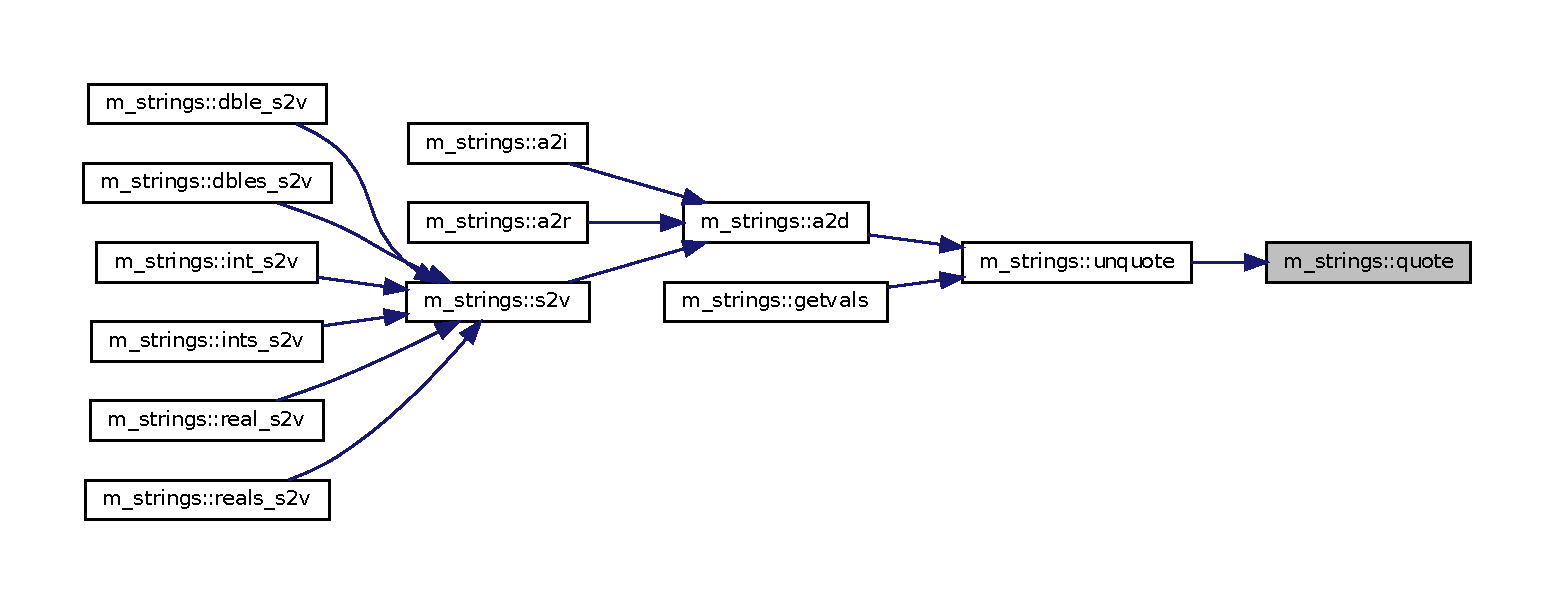
\includegraphics[width=324pt]{namespacem__strings_a3596a4ec755ac897a1dbc0b225d5266a_icgraph}
\end{center}
\end{figure}
\mbox{\Hypertarget{namespacem__strings_ab67ea90007b3f2eb308a5fe8d1cf0df1}\label{namespacem__strings_ab67ea90007b3f2eb308a5fe8d1cf0df1}} 
\index{m\+\_\+strings@{m\+\_\+strings}!r2s@{r2s}}
\index{r2s@{r2s}!m\+\_\+strings@{m\+\_\+strings}}
\subsubsection{\texorpdfstring{r2s()}{r2s()}}
{\footnotesize\ttfamily character(len=\+:) function, allocatable, private m\+\_\+strings\+::r2s (\begin{DoxyParamCaption}\item[{\mbox{\hyperlink{interfacem__strings_1_1real}{real}}, intent(in)}]{rvalue,  }\item[{character(len=$\ast$), intent(in), optional}]{fmt }\end{DoxyParamCaption})\hspace{0.3cm}{\ttfamily [private]}}



References fmt(), and value\+\_\+to\+\_\+string().

Here is the call graph for this function\+:
\nopagebreak
\begin{figure}[H]
\begin{center}
\leavevmode
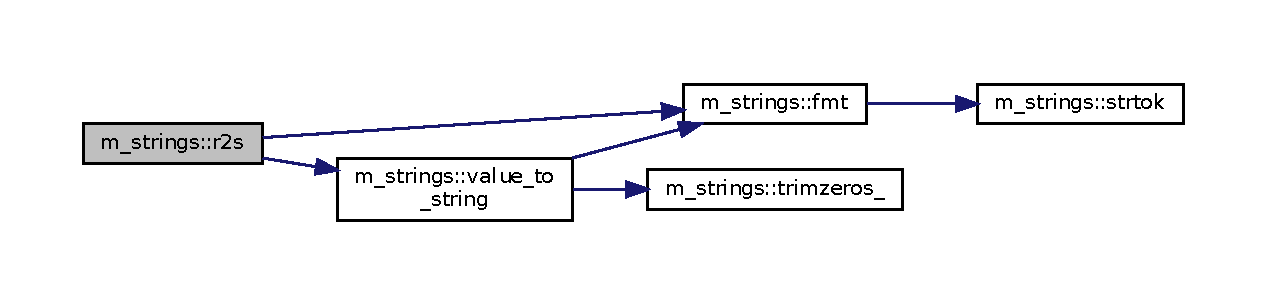
\includegraphics[width=350pt]{namespacem__strings_ab67ea90007b3f2eb308a5fe8d1cf0df1_cgraph}
\end{center}
\end{figure}
\mbox{\Hypertarget{namespacem__strings_aac80fa95c07cf00d5442a88962c5e6e9}\label{namespacem__strings_aac80fa95c07cf00d5442a88962c5e6e9}} 
\index{m\+\_\+strings@{m\+\_\+strings}!real\+\_\+s2v@{real\+\_\+s2v}}
\index{real\+\_\+s2v@{real\+\_\+s2v}!m\+\_\+strings@{m\+\_\+strings}}
\subsubsection{\texorpdfstring{real\+\_\+s2v()}{real\_s2v()}}
{\footnotesize\ttfamily \mbox{\hyperlink{interfacem__strings_1_1real}{real}} function m\+\_\+strings\+::real\+\_\+s2v (\begin{DoxyParamCaption}\item[{character(len=$\ast$), intent(in)}]{chars }\end{DoxyParamCaption})\hspace{0.3cm}{\ttfamily [private]}}

\mbox{\Hypertarget{namespacem__strings_ac62b68d2aeb2b404a3340101f2cb7f84}\label{namespacem__strings_ac62b68d2aeb2b404a3340101f2cb7f84}} 
\index{m\+\_\+strings@{m\+\_\+strings}!reals\+\_\+s2v@{reals\+\_\+s2v}}
\index{reals\+\_\+s2v@{reals\+\_\+s2v}!m\+\_\+strings@{m\+\_\+strings}}
\subsubsection{\texorpdfstring{reals\+\_\+s2v()}{reals\_s2v()}}
{\footnotesize\ttfamily \mbox{\hyperlink{interfacem__strings_1_1real}{real}} function, dimension(\+:), allocatable m\+\_\+strings\+::reals\+\_\+s2v (\begin{DoxyParamCaption}\item[{character(len=$\ast$), dimension(\+:), intent(in)}]{chars }\end{DoxyParamCaption})\hspace{0.3cm}{\ttfamily [private]}}

\mbox{\Hypertarget{namespacem__strings_ab5af73797bb08e7f654d39c9e8984ffe}\label{namespacem__strings_ab5af73797bb08e7f654d39c9e8984ffe}} 
\index{m\+\_\+strings@{m\+\_\+strings}!replace@{replace}}
\index{replace@{replace}!m\+\_\+strings@{m\+\_\+strings}}
\subsubsection{\texorpdfstring{replace()}{replace()}}
{\footnotesize\ttfamily character(len=\+:) function, allocatable, public m\+\_\+strings\+::replace (\begin{DoxyParamCaption}\item[{character(len=$\ast$), intent(in)}]{targetline,  }\item[{character(len=$\ast$), intent(in), optional}]{old,  }\item[{character(len=$\ast$), intent(in), optional}]{new,  }\item[{integer, intent(out), optional}]{ierr,  }\item[{character(len=$\ast$), intent(in), optional}]{cmd,  }\item[{integer, dimension(2), intent(in), optional}]{range }\end{DoxyParamCaption})}



References crack\+\_\+cmd().

Here is the call graph for this function\+:
\nopagebreak
\begin{figure}[H]
\begin{center}
\leavevmode
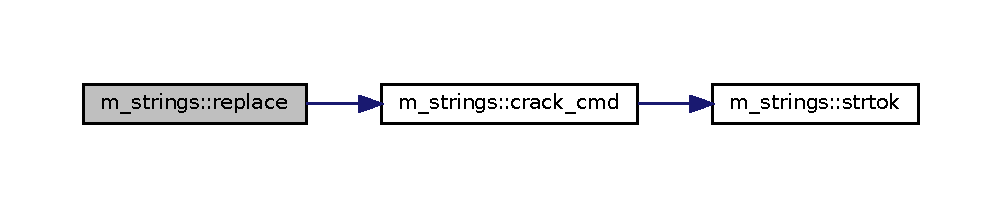
\includegraphics[width=350pt]{namespacem__strings_ab5af73797bb08e7f654d39c9e8984ffe_cgraph}
\end{center}
\end{figure}
Here is the caller graph for this function\+:
\nopagebreak
\begin{figure}[H]
\begin{center}
\leavevmode
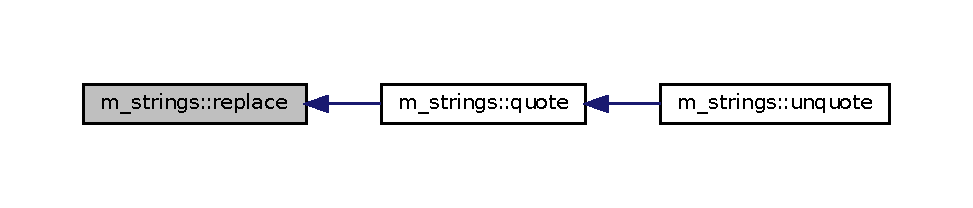
\includegraphics[width=350pt]{namespacem__strings_ab5af73797bb08e7f654d39c9e8984ffe_icgraph}
\end{center}
\end{figure}
\mbox{\Hypertarget{namespacem__strings_ab3e5e7af9e9594fdb544f82736a26f17}\label{namespacem__strings_ab3e5e7af9e9594fdb544f82736a26f17}} 
\index{m\+\_\+strings@{m\+\_\+strings}!reverse@{reverse}}
\index{reverse@{reverse}!m\+\_\+strings@{m\+\_\+strings}}
\subsubsection{\texorpdfstring{reverse()}{reverse()}}
{\footnotesize\ttfamily elemental character(len=len(string)) function, public m\+\_\+strings\+::reverse (\begin{DoxyParamCaption}\item[{character(len=$\ast$), intent(in)}]{string }\end{DoxyParamCaption})}



\subsubsection*{N\+A\+ME}

reverse(3f) -\/ \mbox{[}M\+\_\+strings\+:E\+D\+I\+T\+I\+NG\mbox{]} Return a string reversed (L\+I\+C\+E\+N\+SE\+:PD) 

\subsubsection*{S\+Y\+N\+O\+P\+S\+IS}

\begin{DoxyVerb}elemental pure function reverse(str) result (string)

 character(*), intent(in) :: str
 character(len(str))      :: string
\end{DoxyVerb}
 \subsubsection*{D\+E\+S\+C\+R\+I\+P\+T\+I\+ON}

reverse(string) returns a copy of the input string with all characters reversed from right to left.

\subsubsection*{E\+X\+A\+M\+P\+LE}

Sample program\+: \begin{DoxyVerb} program demo_reverse
 use M_strings, only: reverse
 implicit none
 character(len=:),allocatable  :: s
    write(*,*)'REVERSE STRINGS:',reverse('Madam, I''m Adam')
    s='abcdefghijklmnopqrstuvwxyz'
    write(*,*) 'original input string is ....',s
    write(*,*) 'reversed output string is ...',reverse(s)
 end program demo_reverse
\end{DoxyVerb}


Expected output \begin{DoxyVerb} original input string is ....abcdefghijklmnopqrstuvwxyz
 reversed output string is ...zyxwvutsrqponmlkjihgfedcba
\end{DoxyVerb}
 \subsubsection*{A\+U\+T\+H\+OR}

John S. Urban \subsubsection*{L\+I\+C\+E\+N\+SE}

Public Domain \mbox{\Hypertarget{namespacem__strings_af155dcea0c0ccef21bb359040b673014}\label{namespacem__strings_af155dcea0c0ccef21bb359040b673014}} 
\index{m\+\_\+strings@{m\+\_\+strings}!rotate13@{rotate13}}
\index{rotate13@{rotate13}!m\+\_\+strings@{m\+\_\+strings}}
\subsubsection{\texorpdfstring{rotate13()}{rotate13()}}
{\footnotesize\ttfamily character(len=len(input)) function, public m\+\_\+strings\+::rotate13 (\begin{DoxyParamCaption}\item[{character(len=$\ast$), intent(in)}]{input }\end{DoxyParamCaption})}



\subsubsection*{N\+A\+ME}

rotate13(3f) -\/ \mbox{[}M\+\_\+strings\mbox{]} apply trivial R\+O\+T13 encryption to a string (L\+I\+C\+E\+N\+SE\+:PD) \subsubsection*{S\+Y\+N\+O\+P\+S\+IS}

rotate13(input) result(output)

character(len=$\ast$),intent(in) \+:\+: input character(len=len(input)) \+:\+: output

\subsubsection*{D\+E\+S\+C\+R\+I\+P\+T\+I\+ON}

R\+O\+T13 (\char`\"{}rotate by 13 places\char`\"{}, sometimes hyphenated R\+O\+T-\/13) is a simple letter substitution cipher that replaces a letter with the 13th letter after it in the alphabet; wrapping around if necessary.

The transformation can be done using a lookup table, such as the following\+:

Input A\+B\+C\+D\+E\+F\+G\+H\+I\+J\+K\+L\+M\+N\+O\+P\+Q\+R\+S\+T\+U\+V\+W\+X\+Y\+Zabcdefghijklmnopqrstuvwxyz Output N\+O\+P\+Q\+R\+S\+T\+U\+V\+W\+X\+Y\+Z\+A\+B\+C\+D\+E\+F\+G\+H\+I\+J\+K\+L\+Mnopqrstuvwxyzabcdefghijklm

R\+O\+T13 is used in online forums as a means of hiding spoilers, punchlines, puzzle solutions, and offensive materials from the casual glance. R\+O\+T13 has inspired a variety of letter and word games on-\/line, and is frequently mentioned in newsgroup conversations.

The algorithm provides virtually no cryptographic security, and is often cited as a canonical example of weak encryption.

R\+O\+T13 is a special case of the Caesar cipher which was developed in ancient Rome.

A\+L\+G\+O\+R\+I\+T\+HM

Applying R\+O\+T13 to a piece of text merely requires examining its alphabetic characters and replacing each one by the letter 13 places further along in the alphabet, wrapping back to the beginning if necessary. A becomes N, B becomes O, and so on up to M, which becomes Z, then the sequence continues at the beginning of the alphabet\+: N becomes A, O becomes B, and so on to Z, which becomes M. Only those letters which occur in the English alphabet are affected; numbers, symbols, whitespace, and all other characters are left unchanged.

S\+A\+ME A\+L\+G\+O\+R\+I\+T\+HM F\+OR E\+N\+C\+O\+D\+I\+NG A\+ND D\+E\+C\+O\+D\+I\+NG

Because there are 26 letters in the English alphabet and 26 = 2 x 13, the R\+O\+T13 function is its own inverse\+: so the same action can be used for encoding and decoding. In other words, two successive applications of R\+O\+T13 restore the original text (in mathematics, this is sometimes called an involution; in cryptography, a reciprocal cipher).

T\+R\+I\+V\+I\+AL S\+E\+C\+U\+R\+I\+TY

The use of a constant shift means that the encryption effectively has no key, and decryption requires no more knowledge than the fact that R\+O\+T13 is in use. Even without this knowledge, the algorithm is easily broken through frequency analysis.

In encrypted normal English-\/language text of any significant size, R\+O\+T13 is recognizable from some letter/word patterns. The words \char`\"{}n\char`\"{}, \char`\"{}\+V\char`\"{} (capitalized only), and \char`\"{}gur\char`\"{} (R\+O\+T13 for \char`\"{}a\char`\"{}, \char`\"{}\+I\char`\"{}, and \char`\"{}the\char`\"{}), and words ending in \char`\"{}yl\char`\"{} (\char`\"{}ly\char`\"{}) are examples.

\subsubsection*{R\+E\+F\+E\+R\+E\+N\+C\+ES}

Wikipedia, the free encyclopedia \subsubsection*{E\+X\+A\+M\+P\+LE}

Sample program \begin{DoxyVerb}program demo_rotate13
use M_strings, only : rotate13
implicit none
character(len=256) :: line
integer            :: ios
do
   read(*,'(a)',iostat=ios)line
   if(ios.ne.0)exit
   write(*,'(a)')rotate13(line)
enddo
end program demo_rotate13
\end{DoxyVerb}


Sample usage\+: \begin{DoxyVerb}demo_rotate13
United we stand, divided we fall.
Havgrq jr fgnaq, qvivqrq jr snyy.
\end{DoxyVerb}


\subsubsection*{A\+U\+T\+H\+OR}

John S. Urban \subsubsection*{L\+I\+C\+E\+N\+SE}

Public Domain \mbox{\Hypertarget{namespacem__strings_a5b05f337c8851871a4fb0b3cf56663cd}\label{namespacem__strings_a5b05f337c8851871a4fb0b3cf56663cd}} 
\index{m\+\_\+strings@{m\+\_\+strings}!s2a@{s2a}}
\index{s2a@{s2a}!m\+\_\+strings@{m\+\_\+strings}}
\subsubsection{\texorpdfstring{s2a()}{s2a()}}
{\footnotesize\ttfamily pure character(len=1) function, dimension(len(string)), private m\+\_\+strings\+::s2a (\begin{DoxyParamCaption}\item[{character(len=$\ast$), intent(in)}]{string }\end{DoxyParamCaption})\hspace{0.3cm}{\ttfamily [private]}}

\mbox{\Hypertarget{namespacem__strings_a9a3d38d8e7c4212d63487b9b46bec3b7}\label{namespacem__strings_a9a3d38d8e7c4212d63487b9b46bec3b7}} 
\index{m\+\_\+strings@{m\+\_\+strings}!s2c@{s2c}}
\index{s2c@{s2c}!m\+\_\+strings@{m\+\_\+strings}}
\subsubsection{\texorpdfstring{s2c()}{s2c()}}
{\footnotesize\ttfamily pure character(kind=c\+\_\+char,len=1) function, dimension(len\+\_\+trim(string)+1), public m\+\_\+strings\+::s2c (\begin{DoxyParamCaption}\item[{character(len=$\ast$), intent(in)}]{string }\end{DoxyParamCaption})}



\subsubsection*{N\+A\+ME}

s2c(3f) -\/ \mbox{[}M\+\_\+strings\+:A\+R\+R\+AY\mbox{]} convert character variable to array of characters with last element set to null (L\+I\+C\+E\+N\+SE\+:PD) 

\subsubsection*{S\+Y\+N\+O\+P\+S\+IS}

\begin{DoxyVerb}function s2c(string)

 character(len=*),intent=(in)  :: string
 character(len=1),allocatable  :: s2c(:)
\end{DoxyVerb}
 \subsubsection*{D\+E\+S\+C\+R\+I\+P\+T\+I\+ON}

Given a character variable convert it to an array of single-\/character character variables with the last element set to a null character. This is generally used to pass character variables to C procedures. \subsubsection*{E\+X\+A\+M\+P\+L\+ES}

\begin{DoxyVerb}Sample Program:

    program demo_s2c
    use M_strings, only : s2c
    implicit none
    character(len=*),parameter   :: string="single string"
    character(len=3),allocatable :: array(:)
       write(*,*)'INPUT STRING ',trim(string)
       ! put one character into each 3-character element of array
       array=s2c(string)
       ! write array with ASCII Decimal Equivalent below it except show
       ! unprintable characters like NULL as "XXX"
       write(*,'(1x,*("[",a3,"]":))')&
            & merge('XXX',array,ichar(array(:)(1:1)).lt.32)
       write(*,'(1x,*("[",i3,"]":))')&
            & ichar(array(:)(1:1))
    end program demo_s2c
\end{DoxyVerb}


Expected output\+: \begin{DoxyVerb}INPUT STRING single string
[s  ][i  ][n  ][g  ][l  ][e  ][   ][s  ][t  ][r  ][i  ][n  ][g  ][XXX]
[115][105][110][103][108][101][ 32][115][116][114][105][110][103][  0]
\end{DoxyVerb}


\subsubsection*{A\+U\+T\+H\+OR}

John S. Urban \subsubsection*{L\+I\+C\+E\+N\+SE}

Public Domain \mbox{\Hypertarget{namespacem__strings_ae0e2fe7c93e581402a74a7b59e5bb07f}\label{namespacem__strings_ae0e2fe7c93e581402a74a7b59e5bb07f}} 
\index{m\+\_\+strings@{m\+\_\+strings}!s2v@{s2v}}
\index{s2v@{s2v}!m\+\_\+strings@{m\+\_\+strings}}
\subsubsection{\texorpdfstring{s2v()}{s2v()}}
{\footnotesize\ttfamily doubleprecision function, public m\+\_\+strings\+::s2v (\begin{DoxyParamCaption}\item[{character(len=$\ast$), intent(in)}]{chars,  }\item[{integer, optional}]{ierr,  }\item[{class($\ast$), intent(in), optional}]{onerr }\end{DoxyParamCaption})}



\subsubsection*{N\+A\+ME}

s2v(3f) -\/ \mbox{[}M\+\_\+strings\+:N\+U\+M\+E\+R\+IC\mbox{]} function returns doubleprecision numeric value from a string (L\+I\+C\+E\+N\+SE\+:PD) 

\subsubsection*{S\+Y\+N\+O\+P\+S\+IS}

\begin{DoxyVerb}function s2v(string[,ierr][,onerr])

 character(len=*)             :: string
 doubleprecision              :: s2v
 integer,intent(out),optional :: ierr
 class(*),intent(in),optional :: onerr
\end{DoxyVerb}
 \subsubsection*{D\+E\+S\+C\+R\+I\+P\+T\+I\+ON}

This function converts a string to a D\+O\+U\+B\+L\+E\+P\+R\+E\+C\+I\+S\+I\+ON numeric value.

The intrinsics I\+N\+T(3f), R\+E\+A\+L(3f), and D\+B\+L\+E(3f) are also extended to take C\+H\+A\+R\+A\+C\+T\+ER variables. The K\+I\+ND= keyword is not supported on the extensions. \subsubsection*{O\+P\+T\+I\+O\+NS}

\begin{DoxyVerb} string   holds string assumed to represent a numeric value
 ierr     If an error occurs the program is stopped if the optional
          parameter IERR is not present. If IERR returns a non-zero
          value an error occurred.
 onerr    The value to return on error. A value of NaN is
          returned on error by default.
\end{DoxyVerb}
 \subsubsection*{R\+E\+T\+U\+R\+NS}

s2v

\subsubsection*{E\+X\+A\+M\+P\+LE}

Sample Program\+: \begin{DoxyVerb} program demo_s2v

 use M_strings, only: s2v, int, real, dble
 implicit none
 character(len=8)              :: s=' 10.345 '
 integer                       :: i
 character(len=14),allocatable :: strings(:)
 doubleprecision               :: dv
 integer                       :: errnum

 ! different strings representing INTEGER, REAL, and DOUBLEPRECISION
 strings=[&
 &' 10.345       ',&
 &'+10           ',&
 &'    -3        ',&
 &'    -4.94e-2  ',&
 &'0.1           ',&
 &'12345.678910d0',&
 &'              ',& ! Note: will return zero without an error message
 &'1 2 1 2 1 . 0 ',& ! Note: spaces will be ignored
 &'WHAT?         ']  ! Note: error messages will appear, zero returned

 ! a numeric value is returned, so it can be used in numeric expression
 write(*,*) '1/2 value of string is ',s2v(s)/2.0d0
 write(*,*)
 write(*,*)' STRING            VALUE                    ERROR_NUMBER'
 do i=1,size(strings)
    ! Note: not a good idea to use s2v(3f) in a WRITE(3f) statement,
    ! as it does I/O when errors occur, so called on a separate line
    dv=s2v(strings(i),errnum)
    write(*,*) strings(i)//'=',dv,errnum
 enddo
 write(*,*)"Extended intrinsics"
 write(*,*)'given inputs:',s,strings(:8)
 write(*,*)'INT(3f):',int(s),int(strings(:8))
 write(*,*)'REAL(3f):',real(s),real(strings(:8))
 write(*,*)'DBLE(3f):',dble(s),dble(strings(:8))
 write(*,*)"That's all folks!"

 end program demo_s2v
\end{DoxyVerb}


Expected output

$>$1/2 value of string is 5.\+1725000000000003 $>$ $>$ S\+T\+R\+I\+NG V\+A\+L\+UE E\+R\+R\+O\+R\+\_\+\+N\+U\+M\+B\+ER $>$ 10.\+345 = 10.\+345000000000001 0 $>$+10 = 10.\+000000000000000 0 $>$ -\/3 = -\/3.\+0000000000000000 0 $>$ -\/4.\+94e-\/2 = -\/4.\+9399999999999999E-\/002 0 $>$0.\+1 = 0.\+10000000000000001 0 $>$12345.\+678910d0= 12345.\+678910000001 0 $>$ = 0.\+0000000000000000 0 $>$1 2 1 2 1 . 0 = 12121.\+000000000000 0 $>$$\ast$a2d$\ast$ -\/ cannot produce number from string \mbox{[}W\+H\+AT?\mbox{]} $>$$\ast$a2d$\ast$ -\/ \mbox{[}Bad value during floating point read\mbox{]} $>$W\+H\+AT? = 0.\+0000000000000000 5010 $>$Extended intrinsics $>$given inputs\+: 10.\+345 10.\+345 +10 -\/3 -\/4.\+94e-\/2 0.\+1 12345.\+678910d0 1 2 1 2 1 . 0 $>$I\+N\+T(3f)\+: 10 10 10 -\/3 0 0 12345 0 12121 $>$R\+E\+A\+L(3f)\+: 10.\+3450003 10.\+3450003 10.\+0000000 -\/3.\+00000000 -\/4.\+94000018E-\/02 $>$ 0.\+100000001 12345.\+6787 0.\+00000000 12121.\+0000 $>$D\+B\+L\+E(3f)\+: 10.\+345000000000001 10.\+345000000000001 10.\+000000000000000 $>$ -\/3.\+0000000000000000 -\/4.\+9399999999999999E-\/002 0.\+10000000000000001 $>$ 12345.\+678910000001 0.\+0000000000000000 12121.\+000000000000 $>$That\textquotesingle{}s all folks! \subsubsection*{A\+U\+T\+H\+OR}

John S. Urban \subsubsection*{L\+I\+C\+E\+N\+SE}

Public Domain

\subsubsection*{P\+R\+O\+C\+E\+D\+U\+RE\+:}

D\+E\+S\+C\+R\+I\+P\+T\+I\+ON\+: s2v(3f)\+: function returns doubleprecision number from string;zero if error occurs \subsubsection*{V\+E\+R\+S\+I\+ON\+: 2.\+0, 20160704}

A\+U\+T\+H\+OR\+: John S. Urban 

References a2d().

Here is the call graph for this function\+:
\nopagebreak
\begin{figure}[H]
\begin{center}
\leavevmode
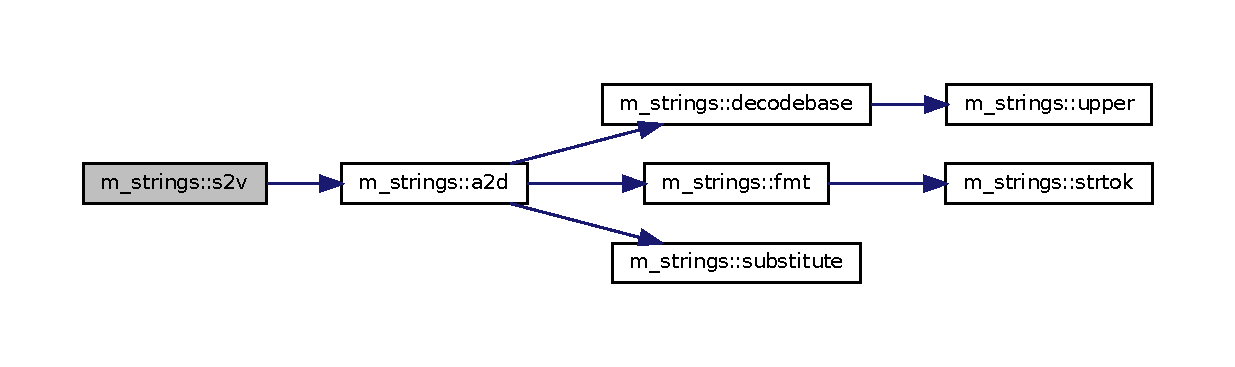
\includegraphics[width=350pt]{namespacem__strings_ae0e2fe7c93e581402a74a7b59e5bb07f_cgraph}
\end{center}
\end{figure}
Here is the caller graph for this function\+:
\nopagebreak
\begin{figure}[H]
\begin{center}
\leavevmode
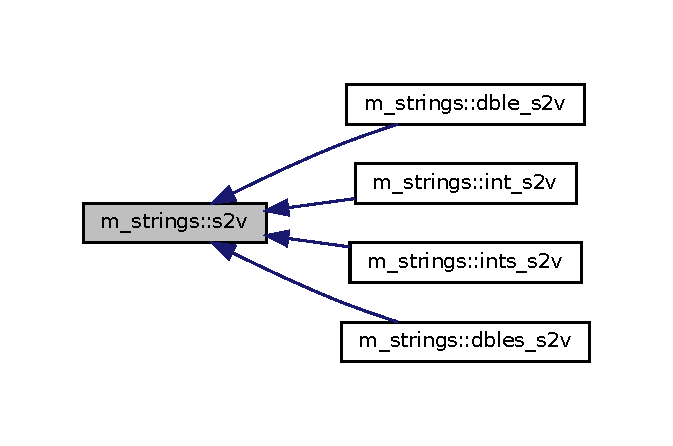
\includegraphics[width=323pt]{namespacem__strings_ae0e2fe7c93e581402a74a7b59e5bb07f_icgraph}
\end{center}
\end{figure}
\mbox{\Hypertarget{namespacem__strings_ad7fffe79559a666aa28e1ed598b8670f}\label{namespacem__strings_ad7fffe79559a666aa28e1ed598b8670f}} 
\index{m\+\_\+strings@{m\+\_\+strings}!s2vs@{s2vs}}
\index{s2vs@{s2vs}!m\+\_\+strings@{m\+\_\+strings}}
\subsubsection{\texorpdfstring{s2vs()}{s2vs()}}
{\footnotesize\ttfamily doubleprecision function, dimension(\+:), allocatable, public m\+\_\+strings\+::s2vs (\begin{DoxyParamCaption}\item[{character(len=$\ast$), intent(in)}]{string,  }\item[{character(len=$\ast$), optional}]{delim }\end{DoxyParamCaption})}



\subsubsection*{N\+A\+ME}

s2vs(3f) -\/ \mbox{[}M\+\_\+strings\+:N\+U\+M\+E\+R\+IC\mbox{]} given a string representing numbers return a numeric array (L\+I\+C\+E\+N\+SE\+:PD) 

\subsubsection*{S\+Y\+N\+O\+P\+S\+IS}

\begin{DoxyVerb}   function s2vs(line[,delim])

    character(len=*) :: line
    doubleprecision,allocatable :: s2vs(:)
\end{DoxyVerb}
 \subsubsection*{D\+E\+S\+C\+R\+I\+P\+T\+I\+ON}

\begin{DoxyVerb}The function S2VS(3f) takes a string representing a series of numbers
and converts it to a numeric doubleprecision array. The string values
may be delimited by spaces, semi-colons, and commas by default.
\end{DoxyVerb}


\subsubsection*{O\+P\+T\+I\+O\+NS}

L\+I\+NE Input string containing numbers D\+E\+L\+IM optional list of delimiter characters. If a space is included, it should appear as the left-\/most character in the list. The default is \char`\"{} ;,\char`\"{} (spaces, semi-\/colons, and commas). \subsubsection*{R\+E\+S\+U\+L\+TS}

S2\+VS doubleprecision array

\subsubsection*{E\+X\+A\+M\+P\+LE}

Sample Program\+: \begin{DoxyVerb} program demo_s2vs
 use M_strings, only : s2vs
 character(len=80)           :: s=' 10 20e3;3.45 -400.3e-2;1234; 5678 '
 doubleprecision,allocatable :: values(:)
 integer,allocatable         :: ivalues(:)

 values=s2vs(s)
 ivalues=int(s2vs(s))
 call reportit()

 contains
   subroutine reportit()
     write(*,*)'S2VS:'
     write(*,*)'input string.............',trim(s)
     write(*,*)'number of values found...',size(values)
     write(*,*)'values...................',(values(ii),ii=1,size(values))
     write(*,*)'ivalues..................',(ivalues(ii),ii=1,size(values))
   end subroutine reportit
 end program demo_s2vs
\end{DoxyVerb}


Expected output \begin{DoxyVerb}S2VS:
input string............. 10 20e3;3.45 -400.3e-2;1234; 5678
number of values found... 6
values................... 10.000000000000000  20000.000000000000 3.4500000000000002
-4.0030000000000001       1234.0000000000000  5678.0000000000000
ivalues.................. 10  20000  3  -4 1234 5678
\end{DoxyVerb}
 \subsubsection*{A\+U\+T\+H\+OR}

John S. Urban \subsubsection*{L\+I\+C\+E\+N\+SE}

Public Domain 

References delim(), and split().

Here is the call graph for this function\+:
\nopagebreak
\begin{figure}[H]
\begin{center}
\leavevmode
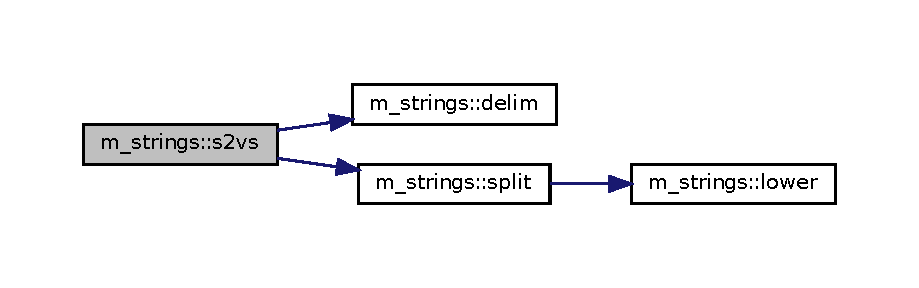
\includegraphics[width=350pt]{namespacem__strings_ad7fffe79559a666aa28e1ed598b8670f_cgraph}
\end{center}
\end{figure}
\mbox{\Hypertarget{namespacem__strings_a536b90500130aa47bde4def7ecd5f6aa}\label{namespacem__strings_a536b90500130aa47bde4def7ecd5f6aa}} 
\index{m\+\_\+strings@{m\+\_\+strings}!setbits16@{setbits16}}
\index{setbits16@{setbits16}!m\+\_\+strings@{m\+\_\+strings}}
\subsubsection{\texorpdfstring{setbits16()}{setbits16()}}
{\footnotesize\ttfamily integer(kind=int16) function, public m\+\_\+strings\+::setbits16 (\begin{DoxyParamCaption}\item[{character(len=16), intent(in)}]{string }\end{DoxyParamCaption})}

\mbox{\Hypertarget{namespacem__strings_a44fd7db30f28fd30086eff1a59fbfa7e}\label{namespacem__strings_a44fd7db30f28fd30086eff1a59fbfa7e}} 
\index{m\+\_\+strings@{m\+\_\+strings}!setbits32@{setbits32}}
\index{setbits32@{setbits32}!m\+\_\+strings@{m\+\_\+strings}}
\subsubsection{\texorpdfstring{setbits32()}{setbits32()}}
{\footnotesize\ttfamily integer(kind=int32) function, public m\+\_\+strings\+::setbits32 (\begin{DoxyParamCaption}\item[{character(len=32), intent(in)}]{string }\end{DoxyParamCaption})}

\mbox{\Hypertarget{namespacem__strings_a3d005819ec07b086dbc6d1c197834142}\label{namespacem__strings_a3d005819ec07b086dbc6d1c197834142}} 
\index{m\+\_\+strings@{m\+\_\+strings}!setbits64@{setbits64}}
\index{setbits64@{setbits64}!m\+\_\+strings@{m\+\_\+strings}}
\subsubsection{\texorpdfstring{setbits64()}{setbits64()}}
{\footnotesize\ttfamily integer(kind=int64) function, public m\+\_\+strings\+::setbits64 (\begin{DoxyParamCaption}\item[{character(len=64), intent(in)}]{string }\end{DoxyParamCaption})}

\mbox{\Hypertarget{namespacem__strings_acc1854720186b8a5582a339d1cbb134b}\label{namespacem__strings_acc1854720186b8a5582a339d1cbb134b}} 
\index{m\+\_\+strings@{m\+\_\+strings}!setbits8@{setbits8}}
\index{setbits8@{setbits8}!m\+\_\+strings@{m\+\_\+strings}}
\subsubsection{\texorpdfstring{setbits8()}{setbits8()}}
{\footnotesize\ttfamily integer(kind=int8) function, public m\+\_\+strings\+::setbits8 (\begin{DoxyParamCaption}\item[{character(len=8), intent(in)}]{string }\end{DoxyParamCaption})}

\mbox{\Hypertarget{namespacem__strings_a3f0119fab962146c7656cad592dd9acd}\label{namespacem__strings_a3f0119fab962146c7656cad592dd9acd}} 
\index{m\+\_\+strings@{m\+\_\+strings}!split@{split}}
\index{split@{split}!m\+\_\+strings@{m\+\_\+strings}}
\subsubsection{\texorpdfstring{split()}{split()}}
{\footnotesize\ttfamily subroutine, public m\+\_\+strings\+::split (\begin{DoxyParamCaption}\item[{character(len=$\ast$), intent(in)}]{input\+\_\+line,  }\item[{character(len=\+:), dimension(\+:), intent(out), allocatable}]{array,  }\item[{character(len=$\ast$), intent(in), optional}]{delimiters,  }\item[{character(len=$\ast$), intent(in), optional}]{order,  }\item[{character(len=$\ast$), intent(in), optional}]{nulls }\end{DoxyParamCaption})}



\subsubsection*{N\+A\+ME}

split(3f) -\/ \mbox{[}M\+\_\+strings\+:T\+O\+K\+E\+NS\mbox{]} parse string into an array using specified delimiters (L\+I\+C\+E\+N\+SE\+:PD) 

\subsubsection*{S\+Y\+N\+O\+P\+S\+IS}

\begin{DoxyVerb}subroutine split(input_line,array,delimiters,order,nulls)

 character(len=*),intent(in)              :: input_line
 character(len=:),allocatable,intent(out) :: array(:)
 character(len=*),optional,intent(in)     :: delimiters
 character(len=*),optional,intent(in)     :: order
 character(len=*),optional,intent(in)     :: nulls
\end{DoxyVerb}
 \subsubsection*{D\+E\+S\+C\+R\+I\+P\+T\+I\+ON}

S\+P\+L\+I\+T(3f) parses a string using specified delimiter characters and store tokens into an allocatable array

\subsubsection*{O\+P\+T\+I\+O\+NS}

\begin{DoxyVerb}INPUT_LINE  Input string to tokenize

ARRAY       Output array of tokens

DELIMITERS  List of delimiter characters.
            The default delimiters are the "whitespace" characters
            (space, tab,new line, vertical tab, formfeed, carriage
            return, and null). You may specify an alternate set of
            delimiter characters.

            Multi-character delimiters are not supported (Each
            character in the DELIMITERS list is considered to be
            a delimiter).

            Quoting of delimiter characters is not supported.

ORDER SEQUENTIAL|REVERSE|RIGHT  Order of output array.
            By default ARRAY contains the tokens having parsed
            the INPUT_LINE from left to right. If ORDER='RIGHT'
            or ORDER='REVERSE' the parsing goes from right to left.

NULLS IGNORE|RETURN|IGNOREEND  Treatment of null fields.
            By default adjacent delimiters in the input string
            do not create an empty string in the output array. if
            NULLS='return' adjacent delimiters create an empty element
            in the output ARRAY. If NULLS='ignoreend' then only
            trailing delimiters at the right of the string are ignored.
\end{DoxyVerb}


\subsubsection*{E\+X\+A\+M\+P\+L\+ES}

Sample program\+: \begin{DoxyVerb} program demo_split
 use M_strings, only: split
 character(len=*),parameter     :: &
 & line='  aBcdef   ghijklmnop qrstuvwxyz  1:|:2     333|333 a B cc    '
 character(len=:),allocatable :: array(:) ! output array of tokens
    write(*,*)'INPUT LINE:['//LINE//']'
    write(*,'(80("="))')
    write(*,*)'typical call:'
    CALL split(line,array)
    write(*,'(i0," ==> ",a)')(i,trim(array(i)),i=1,size(array))
    write(*,*)'SIZE:',SIZE(array)
    write(*,'(80("-"))')
    write(*,*)'custom list of delimiters (colon and vertical line):'
    CALL split(line,array,delimiters=':|',order='sequential',nulls='ignore')
    write(*,'(i0," ==> ",a)')(i,trim(array(i)),i=1,size(array))
    write(*,*)'SIZE:',SIZE(array)
    write(*,'(80("-"))')
    write(*,*)&
  &'custom list of delimiters, reverse array order and count null fields:'
    CALL split(line,array,delimiters=':|',order='reverse',nulls='return')
    write(*,'(i0," ==> ",a)')(i,trim(array(i)),i=1,size(array))
    write(*,*)'SIZE:',SIZE(array)
    write(*,'(80("-"))')
    write(*,*)'INPUT LINE:['//LINE//']'
    write(*,*)&
    &'default delimiters and reverse array order and return null fields:'
    CALL split(line,array,delimiters='',order='reverse',nulls='return')
    write(*,'(i0," ==> ",a)')(i,trim(array(i)),i=1,size(array))
    write(*,*)'SIZE:',SIZE(array)
 end program demo_split
\end{DoxyVerb}


Output

$>$ I\+N\+P\+UT L\+I\+NE\+:\mbox{[} a\+Bcdef ghijklmnop qrstuvwxyz 1\+:$\vert$\+:2 333$\vert$333 a B cc \mbox{]} $>$ =========================================================================== $>$ typical call\+: $>$ 1 ==$>$ a\+Bcdef $>$ 2 ==$>$ ghijklmnop $>$ 3 ==$>$ qrstuvwxyz $>$ 4 ==$>$ 1\+:$\vert$\+:2 $>$ 5 ==$>$ 333$\vert$333 $>$ 6 ==$>$ a $>$ 7 ==$>$ B $>$ 8 ==$>$ cc $>$ S\+I\+ZE\+: 8 $>$ -\/-\/-\/-\/-\/-\/-\/-\/-\/-\/-\/-\/-\/-\/-\/-\/-\/-\/-\/-\/-\/-\/-\/-\/-\/-\/-\/-\/-\/-\/-\/-\/-\/-\/-\/-\/-\/-\/-\/-\/-\/-\/-\/-\/-\/-\/-\/-\/-\/-\/-\/-\/-\/-\/-\/-\/-\/-\/-\/-\/-\/-\/-\/-\/-\/-\/-\/-\/-\/-\/-\/--- $>$ custom list of delimiters (colon and vertical line)\+: $>$ 1 ==$>$ a\+Bcdef ghijklmnop qrstuvwxyz 1 $>$ 2 ==$>$ 2 333 $>$ 3 ==$>$ 333 a B cc $>$ S\+I\+ZE\+: 3 $>$ -\/-\/-\/-\/-\/-\/-\/-\/-\/-\/-\/-\/-\/-\/-\/-\/-\/-\/-\/-\/-\/-\/-\/-\/-\/-\/-\/-\/-\/-\/-\/-\/-\/-\/-\/-\/-\/-\/-\/-\/-\/-\/-\/-\/-\/-\/-\/-\/-\/-\/-\/-\/-\/-\/-\/-\/-\/-\/-\/-\/-\/-\/-\/-\/-\/-\/-\/-\/-\/-\/-\/--- $>$ custom list of delimiters, reverse array order and return null fields\+: $>$ 1 ==$>$ 333 a B cc $>$ 2 ==$>$ 2 333 $>$ 3 ==$>$ $>$ 4 ==$>$ $>$ 5 ==$>$ a\+Bcdef ghijklmnop qrstuvwxyz 1 $>$ S\+I\+ZE\+: 5 $>$ -\/-\/-\/-\/-\/-\/-\/-\/-\/-\/-\/-\/-\/-\/-\/-\/-\/-\/-\/-\/-\/-\/-\/-\/-\/-\/-\/-\/-\/-\/-\/-\/-\/-\/-\/-\/-\/-\/-\/-\/-\/-\/-\/-\/-\/-\/-\/-\/-\/-\/-\/-\/-\/-\/-\/-\/-\/-\/-\/-\/-\/-\/-\/-\/-\/-\/-\/-\/-\/-\/-\/--- $>$ I\+N\+P\+UT L\+I\+NE\+:\mbox{[} a\+Bcdef ghijklmnop qrstuvwxyz 1\+:$\vert$\+:2 333$\vert$333 a B cc \mbox{]} $>$ default delimiters and reverse array order and count null fields\+: $>$ 1 ==$>$ $>$ 2 ==$>$ $>$ 3 ==$>$ $>$ 4 ==$>$ cc $>$ 5 ==$>$ B $>$ 6 ==$>$ a $>$ 7 ==$>$ 333$\vert$333 $>$ 8 ==$>$ $>$ 9 ==$>$ $>$ 10 ==$>$ $>$ 11 ==$>$ $>$ 12 ==$>$ 1\+:$\vert$\+:2 $>$ 13 ==$>$ $>$ 14 ==$>$ qrstuvwxyz $>$ 15 ==$>$ ghijklmnop $>$ 16 ==$>$ $>$ 17 ==$>$ $>$ 18 ==$>$ a\+Bcdef $>$ 19 ==$>$ $>$ 20 ==$>$ $>$ S\+I\+ZE\+: 20 \subsubsection*{A\+U\+T\+H\+OR}

John S. Urban \subsubsection*{L\+I\+C\+E\+N\+SE}

Public Domain 

References lower().

Here is the call graph for this function\+:
\nopagebreak
\begin{figure}[H]
\begin{center}
\leavevmode
\includegraphics[width=306pt]{namespacem__strings_a3f0119fab962146c7656cad592dd9acd_cgraph}
\end{center}
\end{figure}
Here is the caller graph for this function\+:
\nopagebreak
\begin{figure}[H]
\begin{center}
\leavevmode
\includegraphics[width=301pt]{namespacem__strings_a3f0119fab962146c7656cad592dd9acd_icgraph}
\end{center}
\end{figure}
\mbox{\Hypertarget{namespacem__strings_aa67b36ec70dbad84672d3069882929c5}\label{namespacem__strings_aa67b36ec70dbad84672d3069882929c5}} 
\index{m\+\_\+strings@{m\+\_\+strings}!stretch@{stretch}}
\index{stretch@{stretch}!m\+\_\+strings@{m\+\_\+strings}}
\subsubsection{\texorpdfstring{stretch()}{stretch()}}
{\footnotesize\ttfamily character(len=\+:) function, allocatable, public m\+\_\+strings\+::stretch (\begin{DoxyParamCaption}\item[{character(len=$\ast$), intent(in)}]{line,  }\item[{integer, intent(in)}]{length,  }\item[{character(len=$\ast$), intent(in), optional}]{pattern,  }\item[{character(len=$\ast$), intent(in), optional}]{suffix }\end{DoxyParamCaption})}



\subsubsection*{N\+A\+ME}

stretch(3f) -\/ \mbox{[}M\+\_\+strings\+:L\+E\+N\+G\+TH\mbox{]} return string padded to at least specified length (L\+I\+C\+E\+N\+SE\+:PD) 

\subsubsection*{S\+Y\+N\+O\+P\+S\+IS}

\begin{DoxyVerb}function stretch(str,length,pattern,suffix) result(strout)

 character(len=*),intent(in)         :: str
 integer,intent(in)                  :: length
 character(len=*)intent(in),optional :: pattern
 character(len=*)intent(in),optional :: suffix
 character(len=:),allocatable        :: strout
\end{DoxyVerb}
 \subsubsection*{D\+E\+S\+C\+R\+I\+P\+T\+I\+ON}

stretch(3f) pads a string with spaces to at least the specified length. If the trimmed input string is longer than the requested length the original string is returned trimmed of trailing spaces. \subsubsection*{O\+P\+T\+I\+O\+NS}

str the input string to return trimmed, but then padded to the specified length if shorter than length length The minimum string length to return pattern optional string to use as padding. Defaults to a space. suffix optional string to append to output string \subsubsection*{R\+E\+T\+U\+R\+NS}

strout The input string padded to the requested length or the trimmed input string if the input string is longer than the requested length.

\subsubsection*{E\+X\+A\+M\+P\+LE}

Sample Program\+: \begin{DoxyVerb} program demo_stretch
  use M_strings, only : stretch
  implicit none
  character(len=10)            :: string='abcdefghij'
  character(len=:),allocatable :: answer
  integer                      :: i
     answer=stretch(string,5)
     write(*,'("[",a,"]")') answer
     answer=stretch(string,20)
     write(*,'("[",a,"]")') answer
     i=30
     write(*,*)
     write(*,'(1x,a,i0)') stretch('CHAPTER 1 : The beginning ',i,'.'), 1
     write(*,'(1x,a,i0)') stretch('CHAPTER 2 : The end ',i,'.'),       1234
     write(*,'(1x,a,i0)') stretch('APPENDIX ',i,'.'),                  1235
     write(*,*)
     write(*,'(1x,a,i7)') stretch('CHAPTER 1 : The beginning ',i,'.'), 1
     write(*,'(1x,a,i7)') stretch('CHAPTER 2 : The end ',i,'.'),       1234
     write(*,'(1x,a,i7)') stretch('APPENDIX ',i,'.'),                  1235
     write(*,*)
     write(*,*) stretch('CHAPTER 1 : The beginning ',i,suffix=': '), 1
     write(*,*) stretch('CHAPTER 2 : The end ',i,suffix=': '),       1234
     write(*,*) stretch('APPENDIX ',i,suffix=': '),                  1235
 end program demo_stretch
\end{DoxyVerb}


Results\+: \begin{DoxyVerb}[abcdefghij]
[abcdefghij          ]

 CHAPTER 1 : The beginning ....1
 CHAPTER 2 : The end ..........1234
 APPENDIX .....................1235

 CHAPTER 1 : The beginning ....      1
 CHAPTER 2 : The end ..........   1234
 APPENDIX .....................   1235

 CHAPTER 1 : The beginning     :            1
 CHAPTER 2 : The end           :         1234
 APPENDIX                      :         1235
\end{DoxyVerb}


\subsubsection*{A\+U\+T\+H\+OR}

John S. Urban \subsubsection*{L\+I\+C\+E\+N\+SE}

Public Domain 

References atleast().

Here is the call graph for this function\+:
\nopagebreak
\begin{figure}[H]
\begin{center}
\leavevmode
\includegraphics[width=324pt]{namespacem__strings_aa67b36ec70dbad84672d3069882929c5_cgraph}
\end{center}
\end{figure}
\mbox{\Hypertarget{namespacem__strings_af3767887ce5c2373a6d9061ea6664bfc}\label{namespacem__strings_af3767887ce5c2373a6d9061ea6664bfc}} 
\index{m\+\_\+strings@{m\+\_\+strings}!string\+\_\+to\+\_\+values@{string\+\_\+to\+\_\+values}}
\index{string\+\_\+to\+\_\+values@{string\+\_\+to\+\_\+values}!m\+\_\+strings@{m\+\_\+strings}}
\subsubsection{\texorpdfstring{string\+\_\+to\+\_\+values()}{string\_to\_values()}}
{\footnotesize\ttfamily subroutine, public m\+\_\+strings\+::string\+\_\+to\+\_\+values (\begin{DoxyParamCaption}\item[{character(len=$\ast$), intent(in)}]{line,  }\item[{integer, intent(in)}]{iread,  }\item[{\mbox{\hyperlink{interfacem__strings_1_1real}{real}}, dimension(iread), intent(inout)}]{values,  }\item[{integer, intent(out)}]{inums,  }\item[{character(len=$\ast$), intent(in)}]{delims,  }\item[{integer, intent(out)}]{ierr }\end{DoxyParamCaption})}



\subsubsection*{N\+A\+ME}

string\+\_\+to\+\_\+values(3f) -\/ \mbox{[}M\+\_\+strings\+:N\+U\+M\+E\+R\+IC\mbox{]} read a string representing numbers into a numeric array (L\+I\+C\+E\+N\+SE\+:PD) 

\subsubsection*{S\+Y\+N\+O\+P\+S\+IS}

\begin{DoxyVerb}   subroutine string_to_values(line,iread,values,inums,delims,ierr)

    character(len=*) :: line
    integer          :: iread
    real             :: values(*)
    integer          :: inums
    character(len=*) :: delims
    integer          :: ierr
\end{DoxyVerb}
 \subsubsection*{D\+E\+S\+C\+R\+I\+P\+T\+I\+ON}

This routine can take a string representing a series of numbers and convert it to a numeric array and return how many numbers were found.

\subsubsection*{O\+P\+T\+I\+O\+NS}

\begin{DoxyVerb}   LINE     Input string containing numbers
   IREAD    maximum number of values to try to read from input string
\end{DoxyVerb}


\subsubsection*{R\+E\+S\+U\+L\+TS}

\begin{DoxyVerb}   VALUES   real array to be filled with numbers
   INUMS    number of values successfully read (before error occurs
            if one does)
   DELIMS   delimiter character(s), usually a space. must not be a
            null string. If more than one character, a space must
            not be the last character or it will be ignored.
   IERR     error flag (0=no error, else column number string starts
            at that error occurred on).
\end{DoxyVerb}


\subsubsection*{E\+X\+A\+M\+P\+LE}

Sample Program\+: \begin{DoxyVerb}  program demo_string_to_values
   use M_strings, only : string_to_values
   character(len=80)  :: s=' 10 20e3;3.45 -400.3e-2;1234; 5678 '
   integer,parameter  :: isz=10
   real               :: array(isz)

   call string_to_values(s,10,array,inums,' ;',ierr)
   call reportit()

   call string_to_values('10;2.3;3.1416',isz,array,inums,' ;',ierr)
   call reportit()

   contains
      subroutine reportit()
         write(*,*)'string_to_values:'
         write(*,*)'input string.............',trim(s)
         write(*,*)'number of values found...',inums
         write(*,*)'values...................',(array(ii),ii=1,inums)
      end subroutine reportit
  end program demo_string_to_values
\end{DoxyVerb}


Expected output \begin{DoxyVerb}string_to_values:
input string............. 10 20e3;3.45 -400.3e-2;1234; 5678
number of values found...           6
values...................   10.0000000  20000.0000  3.45000005  -4.00299978  1234.00000  5678.00000
string_to_values:
input string............. 10 20e3;3.45 -400.3e-2;1234; 5678
number of values found...           3
values...................   10.0000000  2.29999995  3.14159989
\end{DoxyVerb}
 \subsubsection*{A\+U\+T\+H\+OR}

John S. Urban \subsubsection*{L\+I\+C\+E\+N\+SE}

Public Domain \mbox{\Hypertarget{namespacem__strings_aa53af9135873e241c487a75a7073bda1}\label{namespacem__strings_aa53af9135873e241c487a75a7073bda1}} 
\index{m\+\_\+strings@{m\+\_\+strings}!strtok@{strtok}}
\index{strtok@{strtok}!m\+\_\+strings@{m\+\_\+strings}}
\subsubsection{\texorpdfstring{strtok()}{strtok()}}
{\footnotesize\ttfamily logical function, public m\+\_\+strings\+::strtok (\begin{DoxyParamCaption}\item[{character(len=$\ast$), intent(in)}]{source\+\_\+string,  }\item[{integer, intent(inout)}]{itoken,  }\item[{integer, intent(out)}]{token\+\_\+start,  }\item[{integer, intent(inout)}]{token\+\_\+end,  }\item[{character(len=$\ast$), intent(in)}]{delimiters }\end{DoxyParamCaption})}



\subsubsection*{N\+A\+ME}

strtok(3f) -\/ \mbox{[}M\+\_\+strings\+:T\+O\+K\+E\+NS\mbox{]} Tokenize a string (L\+I\+C\+E\+N\+SE\+:PD) \subsubsection*{S\+Y\+N\+O\+P\+S\+IS}

function strtok(source\+\_\+string,itoken,token\+\_\+start,token\+\_\+end,delimiters) result(strtok\+\_\+status)

logical \+:\+: strtok\+\_\+status ! returned value character(len=$\ast$),intent(in) \+:\+: source\+\_\+string ! string to tokenize integer,intent(inout) \+:\+: itoken ! token count since started integer,intent(out) \+:\+: token\+\_\+start ! beginning of token integer,intent(inout) \+:\+: token\+\_\+end ! end of token character(len=$\ast$),intent(in) \+:\+: delimiters ! list of separator characters

\subsubsection*{D\+E\+S\+C\+R\+I\+P\+T\+I\+ON}

The S\+T\+R\+T\+O\+K(3f) function is used to isolate sequential tokens in a string, S\+O\+U\+R\+C\+E\+\_\+\+S\+T\+R\+I\+NG. These tokens are delimited in the string by at least one of the characters in D\+E\+L\+I\+M\+I\+T\+E\+RS. The first time that S\+T\+R\+T\+O\+K(3f) is called, I\+T\+O\+K\+EN should be specified as zero. Subsequent calls, wishing to obtain further tokens from the same string, should pass back in T\+O\+K\+E\+N\+\_\+\+E\+ND and I\+T\+O\+K\+EN until the function result returns .false.

This routine assumes no other calls are made to it using any other input string while it is processing an input line.

\subsubsection*{O\+P\+T\+I\+O\+NS}

source\+\_\+string input string to parse itoken token count should be set to zero for a new string delimiters characters used to determine the end of tokens \subsubsection*{R\+E\+T\+U\+RN}

token\+\_\+start beginning position in S\+O\+U\+R\+C\+E\+\_\+\+S\+T\+R\+I\+NG where token was found token\+\_\+end ending position in S\+O\+U\+R\+C\+E\+\_\+\+S\+T\+R\+I\+NG where token was found strtok\+\_\+status

\subsubsection*{E\+X\+A\+M\+P\+L\+ES}

Sample program\+: \begin{DoxyVerb} program demo_strtok
 use M_strings, only : strtok
 character(len=264)          :: inline
 character(len=*),parameter  :: delimiters=' ;,'
 integer                     :: ios
 !
    do                        ! read lines from stdin until end-of-file or error
       read (unit=*,fmt="(a)",iostat=ios) inline
       if(ios.ne.0)stop
       itoken=0 ! must set ITOKEN=0 before looping on strtok(3f) on a new string.
       do while ( strtok(inline,itoken,istart,iend,delimiters) )
          print *, itoken,'TOKEN=['//(inline(istart:iend))//']',istart,iend
       enddo
    enddo
 end program demo_strtok
\end{DoxyVerb}


sample input file \begin{DoxyVerb}  this is a test of strtok; A:B :;,C;;
\end{DoxyVerb}


sample output file \begin{DoxyVerb} 1  TOKEN=[this]    2   5
 2  TOKEN=[is]      7   8
 3  TOKEN=[a]       10  10
 4  TOKEN=[test]    12  15
 5  TOKEN=[of]      17  18
 6  TOKEN=[strtok]  20  25
 7  TOKEN=[A:B]     28  30
 8  TOKEN=[:]       32  32
 9  TOKEN=[C]       35  35
\end{DoxyVerb}


\subsubsection*{A\+U\+T\+H\+OR}

John S. Urban \subsubsection*{L\+I\+C\+E\+N\+SE}

Public Domain Here is the caller graph for this function\+:
\nopagebreak
\begin{figure}[H]
\begin{center}
\leavevmode
\includegraphics[width=350pt]{namespacem__strings_aa53af9135873e241c487a75a7073bda1_icgraph}
\end{center}
\end{figure}
\mbox{\Hypertarget{namespacem__strings_ab84a4b7c2be211433c2d1b435a87fa32}\label{namespacem__strings_ab84a4b7c2be211433c2d1b435a87fa32}} 
\index{m\+\_\+strings@{m\+\_\+strings}!substitute@{substitute}}
\index{substitute@{substitute}!m\+\_\+strings@{m\+\_\+strings}}
\subsubsection{\texorpdfstring{substitute()}{substitute()}}
{\footnotesize\ttfamily subroutine, public m\+\_\+strings\+::substitute (\begin{DoxyParamCaption}\item[{character(len=$\ast$)}]{targetline,  }\item[{character(len=$\ast$), intent(in)}]{old,  }\item[{character(len=$\ast$), intent(in)}]{new,  }\item[{integer, intent(out), optional}]{ierr,  }\item[{integer, intent(in), optional}]{start,  }\item[{integer, intent(in), optional}]{end }\end{DoxyParamCaption})}



\subsubsection*{N\+A\+ME}

substitute(3f) -\/ \mbox{[}M\+\_\+strings\+:E\+D\+I\+T\+I\+NG\mbox{]} subroutine globally substitutes one substring for another in string (L\+I\+C\+E\+N\+SE\+:PD) 

\subsubsection*{S\+Y\+N\+O\+P\+S\+IS}

\begin{DoxyVerb}subroutine substitute(targetline,old,new,ierr,start,end)

 character(len=*)              :: targetline
 character(len=*),intent(in)   :: old
 character(len=*),intent(in)   :: new
 integer,intent(out),optional  :: ierr
 integer,intent(in),optional   :: start
 integer,intent(in),optional   :: end
\end{DoxyVerb}
 \subsubsection*{D\+E\+S\+C\+R\+I\+P\+T\+I\+ON}

Globally substitute one substring for another in string.

\subsubsection*{O\+P\+T\+I\+O\+NS}

T\+A\+R\+G\+E\+T\+L\+I\+NE input line to be changed. Must be long enough to hold altered output. O\+LD substring to find and replace N\+EW replacement for O\+LD substring I\+E\+RR error code. If I\+ER = -\/1 bad directive, $>$= 0 then count of changes made. S\+T\+A\+RT sets the left margin to be scanned for O\+LD in T\+A\+R\+G\+E\+T\+L\+I\+NE. E\+ND sets the right margin to be scanned for O\+LD in T\+A\+R\+G\+E\+T\+L\+I\+NE.

\subsubsection*{E\+X\+A\+M\+P\+L\+ES}

Sample Program\+: \begin{DoxyVerb}program demo_substitute
use M_strings, only : substitute
implicit none
! must be long enough to hold changed line
character(len=80) :: targetline

targetline='this is the input string'
write(*,*)'ORIGINAL    : '//trim(targetline)

! changes the input to 'THis is THe input string'
call substitute(targetline,'th','TH')
write(*,*)'th => TH    : '//trim(targetline)

! a null old substring means "at beginning of line"
! changes the input to 'BEFORE:this is the input string'
call substitute(targetline,'','BEFORE:')
write(*,*)'"" => BEFORE: '//trim(targetline)

! a null new string deletes occurrences of the old substring
! changes the input to 'ths s the nput strng'
call substitute(targetline,'i','')
write(*,*)'i => ""     : '//trim(targetline)

end program demo_substitute
\end{DoxyVerb}


Expected output \begin{DoxyVerb} ORIGINAL    : this is the input string
 th => TH    : THis is THe input string
 "" => BEFORE: BEFORE:THis is THe input string
 i => ""     : BEFORE:THs s THe nput strng
\end{DoxyVerb}
 \subsubsection*{A\+U\+T\+H\+OR}

John S. Urban \subsubsection*{L\+I\+C\+E\+N\+SE}

Public Domain Here is the caller graph for this function\+:
\nopagebreak
\begin{figure}[H]
\begin{center}
\leavevmode
\includegraphics[width=350pt]{namespacem__strings_ab84a4b7c2be211433c2d1b435a87fa32_icgraph}
\end{center}
\end{figure}
\mbox{\Hypertarget{namespacem__strings_aa896d221112afb3dbc90eeca6075b282}\label{namespacem__strings_aa896d221112afb3dbc90eeca6075b282}} 
\index{m\+\_\+strings@{m\+\_\+strings}!tobase@{tobase}}
\index{tobase@{tobase}!m\+\_\+strings@{m\+\_\+strings}}
\subsubsection{\texorpdfstring{tobase()}{tobase()}}
{\footnotesize\ttfamily character(len=\+:) function, allocatable m\+\_\+strings\+::tobase (\begin{DoxyParamCaption}\item[{integer, intent(in)}]{base,  }\item[{integer, intent(in)}]{number }\end{DoxyParamCaption})\hspace{0.3cm}{\ttfamily [private]}}



References base().

Here is the call graph for this function\+:
\nopagebreak
\begin{figure}[H]
\begin{center}
\leavevmode
\includegraphics[width=350pt]{namespacem__strings_aa896d221112afb3dbc90eeca6075b282_cgraph}
\end{center}
\end{figure}
\mbox{\Hypertarget{namespacem__strings_aded6e43ae13ff21d76c1739f01a40a63}\label{namespacem__strings_aded6e43ae13ff21d76c1739f01a40a63}} 
\index{m\+\_\+strings@{m\+\_\+strings}!todecimal@{todecimal}}
\index{todecimal@{todecimal}!m\+\_\+strings@{m\+\_\+strings}}
\subsubsection{\texorpdfstring{todecimal()}{todecimal()}}
{\footnotesize\ttfamily integer function m\+\_\+strings\+::todecimal (\begin{DoxyParamCaption}\item[{integer, intent(in)}]{base,  }\item[{character($\ast$), intent(in)}]{instr }\end{DoxyParamCaption})\hspace{0.3cm}{\ttfamily [private]}}



References base(), and lower().

Here is the call graph for this function\+:
\nopagebreak
\begin{figure}[H]
\begin{center}
\leavevmode
\includegraphics[width=350pt]{namespacem__strings_aded6e43ae13ff21d76c1739f01a40a63_cgraph}
\end{center}
\end{figure}
\mbox{\Hypertarget{namespacem__strings_aaee428861205782e002f5e7e8fb002f0}\label{namespacem__strings_aaee428861205782e002f5e7e8fb002f0}} 
\index{m\+\_\+strings@{m\+\_\+strings}!transliterate@{transliterate}}
\index{transliterate@{transliterate}!m\+\_\+strings@{m\+\_\+strings}}
\subsubsection{\texorpdfstring{transliterate()}{transliterate()}}
{\footnotesize\ttfamily pure character(len=len(instr)) function, public m\+\_\+strings\+::transliterate (\begin{DoxyParamCaption}\item[{character(len=$\ast$), intent(in)}]{instr,  }\item[{character(len=$\ast$), intent(in)}]{old\+\_\+set,  }\item[{character(len=$\ast$), intent(in)}]{new\+\_\+set }\end{DoxyParamCaption})}



\subsubsection*{N\+A\+ME}

transliterate(3f) -\/ \mbox{[}M\+\_\+strings\+:E\+D\+I\+T\+I\+NG\mbox{]} replace characters from old set with new set (L\+I\+C\+E\+N\+SE\+:PD) 

\subsubsection*{S\+Y\+N\+O\+P\+S\+IS}

\begin{DoxyVerb}pure function transliterate(instr,old_set,new_set) result(outstr)

 character(len=*),intent(in)  :: instr
 character(len=*),intent(in)  :: old_set
 character(len=*),intent(in)  :: new_set
 character(len=len(instr))    :: outstr
\end{DoxyVerb}
 \subsubsection*{D\+E\+S\+C\+R\+I\+P\+T\+I\+ON}

Translate, squeeze, and/or delete characters from the input string.

\subsubsection*{O\+P\+T\+I\+O\+NS}

instr input string to change old\+\_\+set list of letters to change in I\+N\+S\+TR if found \begin{DoxyVerb}     Each character in the input string that matches a character in
     the old set is replaced.
\end{DoxyVerb}
 new\+\_\+set list of letters to replace letters in O\+L\+D\+\_\+\+S\+ET with. \begin{DoxyVerb}     If the new_set is the empty set the matched characters are deleted.

     If the new_set is shorter than the old set the last character in the
     new set is used to replace the remaining characters in the new set.
\end{DoxyVerb}
 \subsubsection*{R\+E\+T\+U\+R\+NS}

outstr instr with substitutions applied

\subsubsection*{E\+X\+A\+M\+P\+L\+ES}

Sample Program\+: \begin{DoxyVerb}program demo_transliterate

use M_strings, only : transliterate
implicit none
character(len=80)   :: STRING

 STRING='aAbBcCdDeEfFgGhHiIjJkKlLmMnNoOpPqQrRsStTuUvVwWxXyYzZ'
 write(*,'(a)') STRING

 ! convert a string to uppercase:
 write(*,*) TRANSLITERATE(STRING,'abcdefghijklmnopqrstuvwxyz','ABCDEFGHIJKLMNOPQRSTUVWXYZ')

 ! change all miniscule letters to a colon (":"):
 write(*,*) TRANSLITERATE(STRING,'abcdefghijklmnopqrstuvwxyz',':')

 ! delete all miniscule letters
 write(*,*) TRANSLITERATE(STRING,'abcdefghijklmnopqrstuvwxyz','')

end program demo_transliterate
\end{DoxyVerb}


Expected output

$>$ a\+Ab\+Bc\+Cd\+De\+Ef\+Fg\+Gh\+Hi\+Ij\+Jk\+Kl\+Lm\+Mn\+No\+Op\+Pq\+Qr\+Rs\+St\+Tu\+Uv\+Vw\+Wx\+Xy\+YzZ $>$ A\+A\+B\+B\+C\+C\+D\+D\+E\+E\+F\+F\+G\+G\+H\+H\+I\+I\+J\+J\+K\+K\+L\+L\+M\+M\+N\+N\+O\+O\+P\+P\+Q\+Q\+R\+R\+S\+S\+T\+T\+U\+U\+V\+V\+W\+W\+X\+X\+Y\+Y\+ZZ $>$ \+:A\+:\+B\+:\+C\+:\+D\+:\+E\+:\+F\+:\+G\+:\+H\+:\+I\+:\+J\+:\+K\+:\+L\+:\+M\+:\+N\+:\+O\+:\+P\+:\+Q\+:\+R\+:\+S\+:\+T\+:\+U\+:\+V\+:\+W\+:\+X\+:Y\+:Z $>$ A\+B\+C\+D\+E\+F\+G\+H\+I\+J\+K\+L\+M\+N\+O\+P\+Q\+R\+S\+T\+U\+V\+W\+X\+YZ

\subsubsection*{A\+U\+T\+H\+OR}

John S. Urban \subsubsection*{L\+I\+C\+E\+N\+SE}

Public Domain \mbox{\Hypertarget{namespacem__strings_aedbeefa963a63edc16b10e2a833eb609}\label{namespacem__strings_aedbeefa963a63edc16b10e2a833eb609}} 
\index{m\+\_\+strings@{m\+\_\+strings}!trimzeros\+\_\+@{trimzeros\+\_\+}}
\index{trimzeros\+\_\+@{trimzeros\+\_\+}!m\+\_\+strings@{m\+\_\+strings}}
\subsubsection{\texorpdfstring{trimzeros\+\_\+()}{trimzeros\_()}}
{\footnotesize\ttfamily subroutine, private m\+\_\+strings\+::trimzeros\+\_\+ (\begin{DoxyParamCaption}\item[{character(len=$\ast$)}]{string }\end{DoxyParamCaption})\hspace{0.3cm}{\ttfamily [private]}}



\subsubsection*{N\+A\+ME}

trimzeros\+\_\+(3fp) -\/ \mbox{[}M\+\_\+strings\+:N\+U\+M\+E\+R\+IC\mbox{]} Delete trailing zeros from numeric decimal string (L\+I\+C\+E\+N\+SE\+:PD) \subsubsection*{S\+Y\+N\+O\+P\+S\+IS}

subroutine trimzeros\+\_\+(str)

character(len=$\ast$) \+:\+: str \subsubsection*{D\+E\+S\+C\+R\+I\+P\+T\+I\+ON}

T\+R\+I\+M\+Z\+E\+R\+O\+S\+\_\+(3f) deletes trailing zeros from a string representing a number. If the resulting string would end in a decimal point, one trailing zero is added. \subsubsection*{O\+P\+T\+I\+O\+NS}

str input string will be assumed to be a numeric value and have trailing zeros removed \subsubsection*{E\+X\+A\+M\+P\+L\+ES}

Sample program\+: \begin{DoxyVerb}program demo_trimzeros_
use M_strings, only : trimzeros_
character(len=:),allocatable :: string
   write(*,*)trimzeros_('123.450000000000')
   write(*,*)trimzeros_('12345')
   write(*,*)trimzeros_('12345.')
   write(*,*)trimzeros_('12345.00e3')
end program demo_trimzeros_
\end{DoxyVerb}


\subsubsection*{A\+U\+T\+H\+OR}

John S. Urban \subsubsection*{L\+I\+C\+E\+N\+SE}

Public Domain Here is the caller graph for this function\+:
\nopagebreak
\begin{figure}[H]
\begin{center}
\leavevmode
\includegraphics[width=350pt]{namespacem__strings_aedbeefa963a63edc16b10e2a833eb609_icgraph}
\end{center}
\end{figure}
\mbox{\Hypertarget{namespacem__strings_acb88c65d5df2d5b3e55df2d2dab57390}\label{namespacem__strings_acb88c65d5df2d5b3e55df2d2dab57390}} 
\index{m\+\_\+strings@{m\+\_\+strings}!unquote@{unquote}}
\index{unquote@{unquote}!m\+\_\+strings@{m\+\_\+strings}}
\subsubsection{\texorpdfstring{unquote()}{unquote()}}
{\footnotesize\ttfamily character(len=\+:) function, allocatable, public m\+\_\+strings\+::unquote (\begin{DoxyParamCaption}\item[{character(len=$\ast$), intent(in)}]{quoted\+\_\+str,  }\item[{character(len=1), intent(in), optional}]{esc }\end{DoxyParamCaption})}



\subsubsection*{N\+A\+ME}

unquote(3f) -\/ \mbox{[}M\+\_\+strings\+:Q\+U\+O\+T\+ES\mbox{]} remove quotes from string as if read with list-\/directed input (L\+I\+C\+E\+N\+SE\+:PD) \subsubsection*{S\+Y\+N\+O\+P\+S\+IS}

function unquote(quoted\+\_\+str,esc) result (unquoted\+\_\+str)

character(len=$\ast$),intent(in) \+:\+: quoted\+\_\+str character(len=1),optional,intent(in) \+:\+: esc character(len=\+:),allocatable \+:\+: unquoted\+\_\+str \subsubsection*{D\+E\+S\+C\+R\+I\+P\+T\+I\+ON}

Remove quotes from a C\+H\+A\+R\+A\+C\+T\+ER variable as if it was read using list-\/directed input. This is particularly useful for processing tokens read from input such as C\+SV files.

Fortran can now read using list-\/directed input from an internal file, which should handle quoted strings, but list-\/directed input does not support escape characters, which U\+N\+Q\+U\+O\+T\+E(3f) does. \subsubsection*{O\+P\+T\+I\+O\+NS}

quoted\+\_\+str input string to remove quotes from, using the rules of list-\/directed input (two adjacent quotes inside a quoted region are replaced by a single quote, a single quote or double quote is selected as the delimiter based on which is encountered first going from left to right, ...) esc optional character used to protect the next quote character from being processed as a quote, but simply as a plain character. \subsubsection*{R\+E\+S\+U\+LT}

unquoted\+\_\+str The output string, which is based on removing quotes from quoted\+\_\+str. \subsubsection*{E\+X\+A\+M\+P\+LE}

Sample program\+: \begin{DoxyVerb}program demo_unquote
   use M_strings, only : unquote
   implicit none
   character(len=128)           :: quoted_str
   character(len=:),allocatable :: unquoted_str
   character(len=1),parameter   :: esc='\'
   character(len=1024)          :: msg
   integer                      :: ios
   character(len=1024)          :: dummy
   do
      write(*,'(a)',advance='no')'Enter test string:'
      read(*,'(a)',iostat=ios,iomsg=msg)quoted_str
      if(ios.ne.0)then
         write(*,*)trim(msg)
         exit
      endif

      ! the original string
      write(*,'(a)')'QUOTED       ['//trim(quoted_str)//']'

      ! the string processed by unquote(3f)
      unquoted_str=unquote(trim(quoted_str),esc)
      write(*,'(a)')'UNQUOTED     ['//unquoted_str//']'

      ! read the string list-directed to compare the results
      read(quoted_str,*,iostat=ios,iomsg=msg)dummy
      if(ios.ne.0)then
         write(*,*)trim(msg)
      else
         write(*,'(a)')'LIST DIRECTED['//trim(dummy)//']'
      endif
   enddo
end program demo_unquote
\end{DoxyVerb}


\subsubsection*{A\+U\+T\+H\+OR}

John S. Urban \subsubsection*{L\+I\+C\+E\+N\+SE}

Public Domain 

References quote().

Here is the call graph for this function\+:
\nopagebreak
\begin{figure}[H]
\begin{center}
\leavevmode
\includegraphics[width=350pt]{namespacem__strings_acb88c65d5df2d5b3e55df2d2dab57390_cgraph}
\end{center}
\end{figure}
\mbox{\Hypertarget{namespacem__strings_a0953ac5c4d31339fdd8ec3acc9c3c915}\label{namespacem__strings_a0953ac5c4d31339fdd8ec3acc9c3c915}} 
\index{m\+\_\+strings@{m\+\_\+strings}!upper@{upper}}
\index{upper@{upper}!m\+\_\+strings@{m\+\_\+strings}}
\subsubsection{\texorpdfstring{upper()}{upper()}}
{\footnotesize\ttfamily elemental pure character(len(str)) function, public m\+\_\+strings\+::upper (\begin{DoxyParamCaption}\item[{character($\ast$), intent(in)}]{str,  }\item[{integer, intent(in), optional}]{begin,  }\item[{integer, intent(in), optional}]{end }\end{DoxyParamCaption})}



\subsubsection*{N\+A\+ME}

upper(3f) -\/ \mbox{[}M\+\_\+strings\+:C\+A\+SE\mbox{]} changes a string to uppercase (L\+I\+C\+E\+N\+SE\+:PD) 

\subsubsection*{S\+Y\+N\+O\+P\+S\+IS}

\begin{DoxyVerb}elemental pure function upper(str,begin,end) result (string)

 character(*), intent(in)    :: str
 integer,optional,intent(in) :: begin,end
 character(len(str))         :: string  ! output string
\end{DoxyVerb}
 \subsubsection*{D\+E\+S\+C\+R\+I\+P\+T\+I\+ON}

upper(string) returns a copy of the input string with all characters converted in the optionally specified range to uppercase, assuming A\+S\+C\+II character sets are being used. If no range is specified the entire string is converted to uppercase.

\subsubsection*{O\+P\+T\+I\+O\+NS}

str string to convert to uppercase begin optional starting position in \char`\"{}str\char`\"{} to begin converting to uppercase end optional ending position in \char`\"{}str\char`\"{} to stop converting to uppercase

\subsubsection*{R\+E\+S\+U\+L\+TS}

upper copy of the input string with all characters converted to uppercase over optionally specified range.

\subsubsection*{T\+R\+I\+V\+IA}

The terms \char`\"{}uppercase\char`\"{} and \char`\"{}lowercase\char`\"{} date back to the early days of the mechanical printing press. Individual metal alloy casts of each needed letter, or punctuation symbol, were meticulously added to a press block, by hand, before rolling out copies of a page. These metal casts were stored and organized in wooden cases. The more often needed miniscule letters were placed closer to hand, in the lower cases of the work bench. The less often needed, capitalized, majuscule letters, ended up in the harder to reach upper cases.

\subsubsection*{E\+X\+A\+M\+P\+LE}

Sample program\+: \begin{DoxyVerb}program demo_upper
use M_strings, only: upper
implicit none
character(len=:),allocatable  :: s
   s=' ABCDEFG abcdefg '
   write(*,*) 'mixed-case input string is ....',s
   write(*,*) 'upper-case output string is ...',upper(s)
   write(*,*) 'make first character uppercase  ... ',upper('this is a sentence.',1,1)
   write(*,'(1x,a,*(a:,"+"))') 'UPPER(3f) is elemental ==>',upper(["abc","def","ghi"])
end program demo_upper
\end{DoxyVerb}


Expected output \begin{DoxyVerb}mixed-case input string is .... ABCDEFG abcdefg
upper-case output string is ... ABCDEFG ABCDEFG
make first character uppercase  ... This is a sentence.
UPPER(3f) is elemental ==>ABC+DEF+GHI
\end{DoxyVerb}
 \subsubsection*{A\+U\+T\+H\+OR}

John S. Urban \subsubsection*{L\+I\+C\+E\+N\+SE}

Public Domain Here is the caller graph for this function\+:
\nopagebreak
\begin{figure}[H]
\begin{center}
\leavevmode
\includegraphics[width=350pt]{namespacem__strings_a0953ac5c4d31339fdd8ec3acc9c3c915_icgraph}
\end{center}
\end{figure}
\mbox{\Hypertarget{namespacem__strings_a3bd3b1de054c81fcc18b69afc369fb21}\label{namespacem__strings_a3bd3b1de054c81fcc18b69afc369fb21}} 
\index{m\+\_\+strings@{m\+\_\+strings}!upper\+\_\+quoted@{upper\+\_\+quoted}}
\index{upper\+\_\+quoted@{upper\+\_\+quoted}!m\+\_\+strings@{m\+\_\+strings}}
\subsubsection{\texorpdfstring{upper\+\_\+quoted()}{upper\_quoted()}}
{\footnotesize\ttfamily elemental pure character(len=len(str)) function, public m\+\_\+strings\+::upper\+\_\+quoted (\begin{DoxyParamCaption}\item[{character(len=$\ast$), intent(in)}]{str }\end{DoxyParamCaption})}



\subsubsection*{N\+A\+ME}

upper\+\_\+quoted(3f) -\/ \mbox{[}M\+\_\+strings\+:C\+A\+SE\mbox{]} elemental function converts string to miniscule skipping strings quoted per Fortran syntax rules (L\+I\+C\+E\+N\+SE\+:PD) 

\subsubsection*{S\+Y\+N\+O\+P\+S\+IS}

\begin{DoxyVerb}elemental pure function upper_quoted(str) result (string)

 character(*), intent(in)    :: str
 character(len(str))         :: string  ! output string
\end{DoxyVerb}
 \subsubsection*{D\+E\+S\+C\+R\+I\+P\+T\+I\+ON}

upper\+\_\+quoted(string) returns a copy of the input string with all not-\/quoted characters converted to uppercase, assuming A\+S\+C\+II character sets are being used. The quoting rules are the same as for Fortran source. Either a single or double quote starts a quoted string, and a quote character of the same type is doubled when it appears internally in the quoted string. If a double quote quotes the string single quotes may appear in the quoted string as single characters, and vice-\/versa for single quotes.

\subsubsection*{O\+P\+T\+I\+O\+NS}

str string to convert to uppercase

\subsubsection*{R\+E\+S\+U\+L\+TS}

upper copy of the input string with all unquoted characters converted to uppercase

\subsubsection*{E\+X\+A\+M\+P\+LE}

Sample program\+: \begin{DoxyVerb} program demo_upper_quoted
 use M_strings, only: upper_quoted
 implicit none
 character(len=:),allocatable  :: s
 s=' ABCDEFG abcdefg "Double-Quoted" ''Single-Quoted'' "with "" Quote" everything else'
    write(*,*) 'mixed-case input string is ....',s
    write(*,*) 'upper-case output string is ...',upper_quoted(s)
    write(*,*) 'make first character uppercase  ... ',upper_quoted('this is a sentence.')
    write(*,'(1x,a,*(a:,"+"))') 'upper_quoted(3f) is elemental ==>',upper_quoted(["abc","def","ghi"])
 end program demo_upper_quoted
\end{DoxyVerb}


Expected output\+: \begin{DoxyVerb}mixed-case input string is .... ABCDEFG abcdefg "Double-Quoted" 'Single-Quoted' "with "" Quote" everything else
upper-case output string is ... ABCDEFG ABCDEFG "Double-Quoted" 'Single-Quoted' "with "" Quote" EVERYTHING ELSE
make first character uppercase  ... THIS IS A SENTENCE.
upper_quoted(3f) is elemental ==>ABC+DEF+GHI
\end{DoxyVerb}
 \subsubsection*{A\+U\+T\+H\+OR}

John S. Urban \subsubsection*{L\+I\+C\+E\+N\+SE}

Public Domain \mbox{\Hypertarget{namespacem__strings_a76a00e3ca7fb7c9b9cadcd484c6e3946}\label{namespacem__strings_a76a00e3ca7fb7c9b9cadcd484c6e3946}} 
\index{m\+\_\+strings@{m\+\_\+strings}!v2s\+\_\+bug@{v2s\+\_\+bug}}
\index{v2s\+\_\+bug@{v2s\+\_\+bug}!m\+\_\+strings@{m\+\_\+strings}}
\subsubsection{\texorpdfstring{v2s\+\_\+bug()}{v2s\_bug()}}
{\footnotesize\ttfamily character(len=\+:) function, allocatable, public m\+\_\+strings\+::v2s\+\_\+bug (\begin{DoxyParamCaption}\item[{class($\ast$), intent(in)}]{gval }\end{DoxyParamCaption})}



\subsubsection*{N\+A\+ME}

v2s(3f) -\/ \mbox{[}M\+\_\+strings\+:N\+U\+M\+E\+R\+IC\mbox{]} return numeric string from a numeric value (L\+I\+C\+E\+N\+SE\+:PD) 

\subsubsection*{S\+Y\+N\+O\+P\+S\+IS}

\begin{DoxyVerb}   function v2s(value) result(outstr)

    integer|real|doubleprecision|logical,intent(in ) :: value
    character(len=:),allocatable :: outstr
    character(len=*),optional,intent(in) :: fmt
\end{DoxyVerb}


\subsubsection*{D\+E\+S\+C\+R\+I\+P\+T\+I\+ON}

\begin{DoxyVerb}v2s(3f) returns a representation of a numeric value as a
string when given a numeric value of type REAL, DOUBLEPRECISION,
INTEGER or LOGICAL. It creates the strings using internal WRITE()
statements. Trailing zeros are removed from non-zero values, and the
string is left-justified.
\end{DoxyVerb}


\subsubsection*{O\+P\+T\+I\+O\+NS}

V\+A\+L\+UE input value to be converted to a string F\+MT format can be explicitly given, but is limited to generating a string of eighty or less characters.

\subsubsection*{R\+E\+T\+U\+R\+NS}

O\+U\+T\+S\+TR returned string representing input value,

\subsubsection*{E\+X\+A\+M\+P\+LE}

Sample Program\+: \begin{DoxyVerb}program demo_v2s
use M_strings, only: v2s
write(*,*) 'The value of 3.0/4.0 is ['//v2s(3.0/4.0)//']'
write(*,*) 'The value of 1234    is ['//v2s(1234)//']'
write(*,*) 'The value of 0d0     is ['//v2s(0d0)//']'
write(*,*) 'The value of .false. is ['//v2s(.false.)//']'
write(*,*) 'The value of .true. is  ['//v2s(.true.)//']'
end program demo_v2s
\end{DoxyVerb}


Expected output \begin{DoxyVerb} The value of 3.0/4.0 is [0.75]
 The value of 1234    is [1234]
 The value of 0d0     is [0]
 The value of .false. is [F]
 The value of .true. is  [T]
\end{DoxyVerb}


\subsubsection*{A\+U\+T\+H\+OR}

John S. Urban \subsubsection*{L\+I\+C\+E\+N\+SE}

Public Domain 

References value\+\_\+to\+\_\+string().

Here is the call graph for this function\+:
\nopagebreak
\begin{figure}[H]
\begin{center}
\leavevmode
\includegraphics[width=350pt]{namespacem__strings_a76a00e3ca7fb7c9b9cadcd484c6e3946_cgraph}
\end{center}
\end{figure}
\mbox{\Hypertarget{namespacem__strings_a5dcd73626c8909c12f8ea29028927a88}\label{namespacem__strings_a5dcd73626c8909c12f8ea29028927a88}} 
\index{m\+\_\+strings@{m\+\_\+strings}!value\+\_\+to\+\_\+string@{value\+\_\+to\+\_\+string}}
\index{value\+\_\+to\+\_\+string@{value\+\_\+to\+\_\+string}!m\+\_\+strings@{m\+\_\+strings}}
\subsubsection{\texorpdfstring{value\+\_\+to\+\_\+string()}{value\_to\_string()}}
{\footnotesize\ttfamily subroutine, public m\+\_\+strings\+::value\+\_\+to\+\_\+string (\begin{DoxyParamCaption}\item[{class($\ast$), intent(in)}]{gval,  }\item[{character(len=$\ast$), intent(out)}]{chars,  }\item[{integer, intent(out), optional}]{length,  }\item[{integer, optional}]{err,  }\item[{character(len=$\ast$), intent(in), optional}]{fmt,  }\item[{logical, intent(in), optional}]{trimz }\end{DoxyParamCaption})}



\subsubsection*{N\+A\+ME}

value\+\_\+to\+\_\+string(3f) -\/ \mbox{[}M\+\_\+strings\+:N\+U\+M\+E\+R\+IC\mbox{]} return numeric string from a numeric value (L\+I\+C\+E\+N\+SE\+:PD) 

\subsubsection*{S\+Y\+N\+O\+P\+S\+IS}

\begin{DoxyVerb}subroutine value_to_string(value,chars[,ilen,ierr,fmt,trimz])

 character(len=*) :: chars  ! minimum of 23 characters required
 !--------
 ! VALUE may be any <em>one</em> of the following types:
 doubleprecision,intent(in)               :: value
 real,intent(in)                          :: value
 integer,intent(in)                       :: value
 logical,intent(in)                       :: value
 !--------
 character(len=*),intent(out)             :: chars
 integer,intent(out),optional             :: ilen
 integer,optional                         :: ierr
 character(len=*),intent(in),optional     :: fmt
 logical,intent(in)                       :: trimz
\end{DoxyVerb}
 \subsubsection*{D\+E\+S\+C\+R\+I\+P\+T\+I\+ON}

\begin{DoxyVerb}value_to_string(3f) returns a numeric representation of a numeric
value in a string given a numeric value of type REAL, DOUBLEPRECISION,
INTEGER or LOGICAL. It creates the string using internal writes. It
then removes trailing zeros from non-zero values, and left-justifies
the string.
\end{DoxyVerb}


\subsubsection*{O\+P\+T\+I\+O\+NS}

V\+A\+L\+UE input value to be converted to a string F\+MT You may specify a specific format that produces a string up to the length of C\+H\+A\+RS; optional. T\+R\+I\+MZ If a format is supplied the default is not to try to trim trailing zeros. Set T\+R\+I\+MZ to .true. to trim zeros from a string assumed to represent a simple numeric value.

\subsubsection*{R\+E\+T\+U\+R\+NS}

C\+H\+A\+RS returned string representing input value, must be at least 23 characters long; or what is required by optional F\+MT if longer. I\+L\+EN position of last non-\/blank character in returned string; optional. I\+E\+RR If not zero, error occurred; optional. \subsubsection*{E\+X\+A\+M\+P\+LE}

Sample program\+: \begin{DoxyVerb}program demo_value_to_string
use M_strings, only: value_to_string
implicit none
character(len=80) :: string
integer           :: ilen
   call value_to_string(3.0/4.0,string,ilen)
   write(*,*) 'The value is [',string(:ilen),']'

   call value_to_string(3.0/4.0,string,ilen,fmt='')
   write(*,*) 'The value is [',string(:ilen),']'

   call value_to_string(3.0/4.0,string,ilen,fmt='("THE VALUE IS ",g0)')
   write(*,*) 'The value is [',string(:ilen),']'

   call value_to_string(1234,string,ilen)
   write(*,*) 'The value is [',string(:ilen),']'

   call value_to_string(1.0d0/3.0d0,string,ilen)
   write(*,*) 'The value is [',string(:ilen),']'

end program demo_value_to_string
\end{DoxyVerb}


Expected output \begin{DoxyVerb}The value is [0.75]
The value is [      0.7500000000]
The value is [THE VALUE IS .750000000]
The value is [1234]
The value is [0.33333333333333331]
\end{DoxyVerb}


\subsubsection*{A\+U\+T\+H\+OR}

John S. Urban \subsubsection*{L\+I\+C\+E\+N\+SE}

Public Domain 

References fmt(), and trimzeros\+\_\+().

Here is the call graph for this function\+:
\nopagebreak
\begin{figure}[H]
\begin{center}
\leavevmode
\includegraphics[width=350pt]{namespacem__strings_a5dcd73626c8909c12f8ea29028927a88_cgraph}
\end{center}
\end{figure}
Here is the caller graph for this function\+:
\nopagebreak
\begin{figure}[H]
\begin{center}
\leavevmode
\includegraphics[width=340pt]{namespacem__strings_a5dcd73626c8909c12f8ea29028927a88_icgraph}
\end{center}
\end{figure}
\mbox{\Hypertarget{namespacem__strings_a791e24ceb690010fd42a6c1f48311b55}\label{namespacem__strings_a791e24ceb690010fd42a6c1f48311b55}} 
\index{m\+\_\+strings@{m\+\_\+strings}!visible@{visible}}
\index{visible@{visible}!m\+\_\+strings@{m\+\_\+strings}}
\subsubsection{\texorpdfstring{visible()}{visible()}}
{\footnotesize\ttfamily character(len=\+:) function, allocatable, public m\+\_\+strings\+::visible (\begin{DoxyParamCaption}\item[{character(len=$\ast$), intent(in)}]{input }\end{DoxyParamCaption})}



\subsubsection*{N\+A\+ME}

visible(3f) -\/ \mbox{[}M\+\_\+strings\+:N\+O\+N\+A\+L\+P\+HA\mbox{]} expand a string to control and meta-\/control representations (L\+I\+C\+E\+N\+SE\+:PD) 

\subsubsection*{S\+Y\+N\+O\+P\+S\+IS}

\begin{DoxyVerb}function visible(input) result(output)

 character(len=*),intent(in)           :: input
 character(len=:),allocatable          :: output
\end{DoxyVerb}
 \subsubsection*{D\+E\+S\+C\+R\+I\+P\+T\+I\+ON}

\begin{DoxyVerb} visible(3f) expands characters to commonly used sequences used to represent the characters
 as control sequences or meta-control sequences.
\end{DoxyVerb}


\subsubsection*{E\+X\+A\+M\+P\+L\+ES}

Sample Program\+: \begin{DoxyVerb} program demo_visible
 use M_strings, only : visible
 integer :: i
    do i=0,255
       write(*,'(i0,1x,a)')i,visible(char(i))
    enddo
 end program demo_visible
\end{DoxyVerb}
 \subsubsection*{B\+U\+GS}

The expansion is not reversible, as input sequences such as \char`\"{}\+M-\/\char`\"{} or \char`\"{}$^\wedge$a\char`\"{} will look like expanded sequences.

\subsubsection*{A\+U\+T\+H\+OR}

John S. Urban \subsubsection*{L\+I\+C\+E\+N\+SE}

Public Domain 

\subsection{Variable Documentation}
\mbox{\Hypertarget{namespacem__strings_ae939ea755cfa377c5ed5f09ba8b0e923}\label{namespacem__strings_ae939ea755cfa377c5ed5f09ba8b0e923}} 
\index{m\+\_\+strings@{m\+\_\+strings}!ascii\+\_\+bel@{ascii\+\_\+bel}}
\index{ascii\+\_\+bel@{ascii\+\_\+bel}!m\+\_\+strings@{m\+\_\+strings}}
\subsubsection{\texorpdfstring{ascii\+\_\+bel}{ascii\_bel}}
{\footnotesize\ttfamily character, parameter, public m\+\_\+strings\+::ascii\+\_\+bel = char(7)}

\mbox{\Hypertarget{namespacem__strings_a6d4b461b6fba6d81e0cee7b6e579c77b}\label{namespacem__strings_a6d4b461b6fba6d81e0cee7b6e579c77b}} 
\index{m\+\_\+strings@{m\+\_\+strings}!ascii\+\_\+bs@{ascii\+\_\+bs}}
\index{ascii\+\_\+bs@{ascii\+\_\+bs}!m\+\_\+strings@{m\+\_\+strings}}
\subsubsection{\texorpdfstring{ascii\+\_\+bs}{ascii\_bs}}
{\footnotesize\ttfamily character, parameter, public m\+\_\+strings\+::ascii\+\_\+bs = char(8)}

\mbox{\Hypertarget{namespacem__strings_a1f58b48efb41665079ced6de505a3b65}\label{namespacem__strings_a1f58b48efb41665079ced6de505a3b65}} 
\index{m\+\_\+strings@{m\+\_\+strings}!ascii\+\_\+cr@{ascii\+\_\+cr}}
\index{ascii\+\_\+cr@{ascii\+\_\+cr}!m\+\_\+strings@{m\+\_\+strings}}
\subsubsection{\texorpdfstring{ascii\+\_\+cr}{ascii\_cr}}
{\footnotesize\ttfamily character, parameter, public m\+\_\+strings\+::ascii\+\_\+cr = char(13)}

\mbox{\Hypertarget{namespacem__strings_a6e9a1f921d2bb4a14a9b50a3b8f96288}\label{namespacem__strings_a6e9a1f921d2bb4a14a9b50a3b8f96288}} 
\index{m\+\_\+strings@{m\+\_\+strings}!ascii\+\_\+esc@{ascii\+\_\+esc}}
\index{ascii\+\_\+esc@{ascii\+\_\+esc}!m\+\_\+strings@{m\+\_\+strings}}
\subsubsection{\texorpdfstring{ascii\+\_\+esc}{ascii\_esc}}
{\footnotesize\ttfamily character, parameter, public m\+\_\+strings\+::ascii\+\_\+esc = char(27)}

\mbox{\Hypertarget{namespacem__strings_a52761941cc3dba4a2ed922d1b7841c90}\label{namespacem__strings_a52761941cc3dba4a2ed922d1b7841c90}} 
\index{m\+\_\+strings@{m\+\_\+strings}!ascii\+\_\+ff@{ascii\+\_\+ff}}
\index{ascii\+\_\+ff@{ascii\+\_\+ff}!m\+\_\+strings@{m\+\_\+strings}}
\subsubsection{\texorpdfstring{ascii\+\_\+ff}{ascii\_ff}}
{\footnotesize\ttfamily character, parameter, public m\+\_\+strings\+::ascii\+\_\+ff = char(12)}

\mbox{\Hypertarget{namespacem__strings_a3fef6116790e59c99f48ea31a7b00133}\label{namespacem__strings_a3fef6116790e59c99f48ea31a7b00133}} 
\index{m\+\_\+strings@{m\+\_\+strings}!ascii\+\_\+ht@{ascii\+\_\+ht}}
\index{ascii\+\_\+ht@{ascii\+\_\+ht}!m\+\_\+strings@{m\+\_\+strings}}
\subsubsection{\texorpdfstring{ascii\+\_\+ht}{ascii\_ht}}
{\footnotesize\ttfamily character, parameter, public m\+\_\+strings\+::ascii\+\_\+ht = char(9)}

\mbox{\Hypertarget{namespacem__strings_a4d65d248433f7c6ea3188c558f795c23}\label{namespacem__strings_a4d65d248433f7c6ea3188c558f795c23}} 
\index{m\+\_\+strings@{m\+\_\+strings}!ascii\+\_\+lf@{ascii\+\_\+lf}}
\index{ascii\+\_\+lf@{ascii\+\_\+lf}!m\+\_\+strings@{m\+\_\+strings}}
\subsubsection{\texorpdfstring{ascii\+\_\+lf}{ascii\_lf}}
{\footnotesize\ttfamily character, parameter, public m\+\_\+strings\+::ascii\+\_\+lf = char(10)}

\mbox{\Hypertarget{namespacem__strings_a9de5098e31c6411a43323b1d7f19a886}\label{namespacem__strings_a9de5098e31c6411a43323b1d7f19a886}} 
\index{m\+\_\+strings@{m\+\_\+strings}!ascii\+\_\+nul@{ascii\+\_\+nul}}
\index{ascii\+\_\+nul@{ascii\+\_\+nul}!m\+\_\+strings@{m\+\_\+strings}}
\subsubsection{\texorpdfstring{ascii\+\_\+nul}{ascii\_nul}}
{\footnotesize\ttfamily character, parameter, public m\+\_\+strings\+::ascii\+\_\+nul = char(0)}


\hypertarget{namespacem__strings__oop}{}\doxysection{m\+\_\+strings\+\_\+oop Module Reference}
\label{namespacem__strings__oop}\index{m\_strings\_oop@{m\_strings\_oop}}
\doxysubsection*{Data Types}
\begin{DoxyCompactItemize}
\item 
interface \mbox{\hyperlink{structm__strings__oop_1_1string}{string}}
\end{DoxyCompactItemize}
\doxysubsection*{Functions/\+Subroutines}
\begin{DoxyCompactItemize}
\item 
type(\mbox{\hyperlink{structm__strings__oop_1_1string}{string}}) function \mbox{\hyperlink{namespacem__strings__oop_a411874cce2f16fee4d05d7528b510703}{construct\+\_\+from\+\_\+fill}} (chars, len)
\item 
integer function \mbox{\hyperlink{namespacem__strings__oop_a768ea13372aadbeae760c72d0b2a1939}{oop\+\_\+len}} (self)
\item 
integer function \mbox{\hyperlink{namespacem__strings__oop_a1b9bf3c6aac71ce1782fb3116ffb63f8}{oop\+\_\+len\+\_\+trim}} (self)
\item 
character(len=1) function, dimension(len(self\%str)) \mbox{\hyperlink{namespacem__strings__oop_a31be80e67fa4829b5ac48c530bd58b7b}{oop\+\_\+switch}} (self)
\item 
integer function \mbox{\hyperlink{namespacem__strings__oop_aafe02b26ccba21eb8a35e9fa99d6c790}{oop\+\_\+index}} (self, substring, back)
\item 
type(\mbox{\hyperlink{structm__strings__oop_1_1string}{string}}) function \mbox{\hyperlink{namespacem__strings__oop_a9f4030a1ab2c7e2aa71b9d1f2754e67e}{oop\+\_\+upper}} (self)
\item 
type(\mbox{\hyperlink{structm__strings__oop_1_1string}{string}}) function \mbox{\hyperlink{namespacem__strings__oop_ad49fed83544ede7b94948dee326ca3d7}{oop\+\_\+lower}} (self)
\item 
type(\mbox{\hyperlink{structm__strings__oop_1_1string}{string}}) function \mbox{\hyperlink{namespacem__strings__oop_a5b96d2a6f242a096cd5788cf0802e825}{oop\+\_\+expand}} (self, escape\+\_\+char)
\item 
type(\mbox{\hyperlink{structm__strings__oop_1_1string}{string}}) function \mbox{\hyperlink{namespacem__strings__oop_ab9238801d6c3af2fe7ee81c8d2c514ff}{oop\+\_\+trim}} (self)
\item 
type(\mbox{\hyperlink{structm__strings__oop_1_1string}{string}}) function \mbox{\hyperlink{namespacem__strings__oop_aa1a395d359592720a842054fd0aaff0a}{oop\+\_\+crop}} (self)
\item 
type(\mbox{\hyperlink{structm__strings__oop_1_1string}{string}}) function \mbox{\hyperlink{namespacem__strings__oop_ac3ab62e14d0b8445f51e084b810e2f76}{oop\+\_\+reverse}} (self)
\item 
type(\mbox{\hyperlink{structm__strings__oop_1_1string}{string}}) function \mbox{\hyperlink{namespacem__strings__oop_a8e2457b4a1c4489e9600e340fa9ce533}{oop\+\_\+adjustl}} (self)
\item 
type(\mbox{\hyperlink{structm__strings__oop_1_1string}{string}}) function \mbox{\hyperlink{namespacem__strings__oop_abb0dfa5646259e4fc768700eada111ac}{oop\+\_\+adjustr}} (self)
\item 
type(\mbox{\hyperlink{structm__strings__oop_1_1string}{string}}) function \mbox{\hyperlink{namespacem__strings__oop_a9fa932c23648e737230553a8e7bfb15b}{oop\+\_\+adjustc}} (self, length)
\item 
integer function \mbox{\hyperlink{namespacem__strings__oop_a2092266bec4014f74b8d436c5a8e319f}{oop\+\_\+int}} (self)
\item 
real function \mbox{\hyperlink{namespacem__strings__oop_a9709a714bc825704651b00c7384a7547}{oop\+\_\+real}} (self)
\item 
doubleprecision function \mbox{\hyperlink{namespacem__strings__oop_aa6eaf2b8a12a905d0ebaa21a84871dec}{oop\+\_\+dble}} (self)
\item 
type(\mbox{\hyperlink{structm__strings__oop_1_1string}{string}}) function \mbox{\hyperlink{namespacem__strings__oop_ac02aecbaebcf57833b544de4f50c89a6}{oop\+\_\+compact}} (self, char)
\item 
type(\mbox{\hyperlink{structm__strings__oop_1_1string}{string}}) function \mbox{\hyperlink{namespacem__strings__oop_af653c84bbd0165d1d4a3b61efe0472e8}{oop\+\_\+substitute}} (self, old, new)
\item 
type(\mbox{\hyperlink{structm__strings__oop_1_1string}{string}}) function \mbox{\hyperlink{namespacem__strings__oop_ac88f27671dd1129023494bf2500ca7fd}{oop\+\_\+transliterate}} (self, old, new)
\item 
type(\mbox{\hyperlink{structm__strings__oop_1_1string}{string}}) function \mbox{\hyperlink{namespacem__strings__oop_a3ee018293cef22d7314b2a9f0c78a319}{oop\+\_\+atleast}} (self, length)
\item 
type(\mbox{\hyperlink{structm__strings__oop_1_1string}{string}}) function \mbox{\hyperlink{namespacem__strings__oop_ac8ca18186659b8759b08e5167a3effb5}{oop\+\_\+lenset}} (self, length)
\item 
logical function \mbox{\hyperlink{namespacem__strings__oop_ab88f5f814c08f1c93c95fcd0ba2a6779}{oop\+\_\+matchw}} (self, pattern)
\item 
type(\mbox{\hyperlink{structm__strings__oop_1_1string}{string}}) function \mbox{\hyperlink{namespacem__strings__oop_a5959b2f967a6466c198b39a089ef8a68}{oop\+\_\+notabs}} (self)
\item 
type(\mbox{\hyperlink{structm__strings__oop_1_1string}{string}}) function \mbox{\hyperlink{namespacem__strings__oop_ae1ed148f1ae0694ac093d3e11f9b702b}{oop\+\_\+noesc}} (self)
\item 
character(len=len(self\%str)) function, public \mbox{\hyperlink{namespacem__strings__oop_a456e651940e317c7bc885d95458c7fcb}{p}} (self)
\item 
subroutine \mbox{\hyperlink{namespacem__strings__oop_a1510c1de10cb182598ce6a399a734be0}{init\+\_\+string}} (self)
\item 
type(\mbox{\hyperlink{structm__strings__oop_1_1string}{string}}) function \mbox{\hyperlink{namespacem__strings__oop_abf27744e539317dac81d6ed1fb736059}{string\+\_\+plus\+\_\+value}} (self, value)
\item 
type(\mbox{\hyperlink{structm__strings__oop_1_1string}{string}}) function \mbox{\hyperlink{namespacem__strings__oop_a0ec84db43ac789bfc02f46f933a3fc9f}{string\+\_\+minus\+\_\+value}} (self, value)
\item 
type(\mbox{\hyperlink{structm__strings__oop_1_1string}{string}}) function \mbox{\hyperlink{namespacem__strings__oop_a64192a93804fcb61ca59725245ee85c2}{string\+\_\+append\+\_\+value}} (self, value)
\item 
type(\mbox{\hyperlink{structm__strings__oop_1_1string}{string}}) function \mbox{\hyperlink{namespacem__strings__oop_a9624f1e09be383f993e7c0e94b230deb}{string\+\_\+multiply\+\_\+value}} (self, value)
\item 
logical function \mbox{\hyperlink{namespacem__strings__oop_a2e5c8d9117609e553db07a1eba18b1fa}{eq}} (self, other)
\item 
logical function \mbox{\hyperlink{namespacem__strings__oop_a332288f9bebc563e12671b514512eb30}{lt}} (self, other)
\item 
logical function \mbox{\hyperlink{namespacem__strings__oop_a25beb184587d7c9fc0a3fd846d4ce187}{gt}} (self, other)
\item 
logical function \mbox{\hyperlink{namespacem__strings__oop_a103e7c1fab92a1c4cbfff87ec8cd1e23}{le}} (self, other)
\item 
logical function \mbox{\hyperlink{namespacem__strings__oop_a2d31ec44898046ba97aebc0de32de19a}{ge}} (self, other)
\item 
logical function \mbox{\hyperlink{namespacem__strings__oop_aa424e1eccc45bb143172d6e212f8e408}{ne}} (self, other)
\end{DoxyCompactItemize}
\doxysubsection*{Variables}
\begin{DoxyCompactItemize}
\item 
integer, parameter, private \mbox{\hyperlink{namespacem__strings__oop_aff89e0d0502f39fedc4f8a9cf793fdba}{dp}} =kind(0.\+0d0)
\end{DoxyCompactItemize}


\doxysubsection{Detailed Description}
\hypertarget{namespacem__strings__oop_autotoc_md545}{}\doxysubsubsection{N\+A\+ME}\label{namespacem__strings__oop_autotoc_md545}
M\+\_\+strings\+\_\+oop(3f) -\/ \mbox{[}M\+\_\+strings\+:I\+N\+T\+RO\mbox{]} O\+OP Fortran string module\hypertarget{namespacem__strings__oop_autotoc_md546}{}\doxysubsubsection{S\+Y\+N\+O\+P\+S\+IS}\label{namespacem__strings__oop_autotoc_md546}
\begin{DoxyVerb}use M_strings_oop
\end{DoxyVerb}
\hypertarget{namespacem__strings__oop_autotoc_md547}{}\doxysubsubsection{D\+E\+S\+C\+R\+I\+P\+T\+I\+ON}\label{namespacem__strings__oop_autotoc_md547}
The M\+\_\+strings(3fm) module is a collection of Fortran procedures that supplement the built-\/in intrinsic string routines. Routines for parsing, tokenizing, changing case, substituting new strings for substrings, locating strings with simple wildcard expressions, removing tabs and line terminators and other string manipulations are included.

M\+\_\+strings\+\_\+oop(3fm) is a companion module that provides an O\+OP interface to the M\+\_\+strings module.\hypertarget{namespacem__strings__oop_autotoc_md548}{}\doxysubsubsection{S\+E\+E A\+L\+SO}\label{namespacem__strings__oop_autotoc_md548}
There are additional routines in other G\+PF modules for working with expressions (M\+\_\+calculator), time strings (M\+\_\+time), random strings (M\+\_\+random, M\+\_\+uuid), lists (M\+\_\+list), and interfacing with the C regular expression library (M\+\_\+regex).\hypertarget{namespacem__strings__oop_autotoc_md549}{}\doxysubsubsection{E\+X\+A\+M\+P\+L\+ES}\label{namespacem__strings__oop_autotoc_md549}
\begin{DoxyVerb}Each of the procedural functions in M_strings(3fm) includes an example
program in the corresponding man(1) page for the function. The
object-oriented interface does not have individual man(1) pages,
but is instead demonstrated using the following example program:

 program demo_M_strings_oop
 !
 ! This is an example using the object-oriented class/type model
 ! defined in M_strings_oop
 ! This is essentially the same functionality as the procedures
 ! combined with several Fortran intrinsics and overloaded operators
 !
 use M_strings_oop,only : string, p
 implicit none
 TYPE(string) :: str1
 TYPE(string) :: str2
 TYPE(string) :: str3
 TYPE(string) :: str4
 !==============================================================================
   write(*,*)'exercise the M_STRING_OOP module interface'
   ! draw a break line in the output
   write(*,*)repeat('=',78)
   write(*,*)'Call methods of type(STRING)'
   ! define TYPE(STRING) with constructor
   str2=string('   This  is  a  String!       ')
   str4=string(' a  String ')
   write(*,*)repeat('=',78)
   ! print members of type
   write(*,101)'str2%str is ................ ',str2%str
   ! same as intrinsic LEN()
   write(*,202)'len ........................ ',str2%len()
   ! same as intrinsic INDEX()
   write(*,202)'len_trim ................... ',str2%len_trim()
   ! same as intrinsic INDEX()
   write(*,202)'index("is")................. ',str2%index("is")
   ! same as intrinsic INDEX()
   write(*,202)'index("is",back=.T.) ....... ',str2%index("is",back=.TRUE.)
   ! output TYPE(STRING) with %str all uppercase
   write(*,101)'upper ...................... ',p(str2%upper())
   ! output TYPE(STRING) with %str all miniscule
   write(*,101)'lower ...................... ',p(str2%lower())
   ! output TYPE(STRING) with %str reversed
   write(*,101)'reverse .................... ',p(str2%reverse())
   ! same as intrinsic ADJUSTL()
   write(*,101)'adjustl .................... ',p(str2%adjustl())
   ! same as intrinsic ADJUSTR()
   write(*,101)'adjustr .................... ',p(str2%adjustr())
   ! center string in current string length
   write(*,101)'adjustc .................... ',p(str2%adjustc())
   ! center string in string length of NN
   write(*,101)'adjustc(49) ................ ',p(str2%adjustc(49))
   ! force %str to be NN characters long
   write(*,101)'lenset(49) ................. ',p(str2%lenset(49))
   ! same as intrinsic TRIM()
   write(*,101)'trim ....................... ',p(str2%trim())
   ! trim leading and trailing spaces
   write(*,101)'crop ....................... ',p(str2%crop())
   ! calls M_strings procedure SUBSTITUTE()
   write(*,101)'substitute("This","Here") .. ',p(str2%substitute("This","Here"))
   ! calls M_strings procedure COMPACT()
   write(*,101)'compact .................... ',p(str2%compact())
   write(*,101)'compact("") ................ ',p(str2%compact(""))
   write(*,101)'compact(":") ............... ',p(str2%compact(":"))
   ! calls M_strings procedure TRANSLITERATE()
   write(*,101)'transliterate("aei","VWX") . ',p(str2%transliterate("aei","VWX"))
   write(*,101)'transliterate("aeiou"," ") . ',p(str2%transliterate("aeiou"," "))
   write(*,101)'transliterate("aeiou","") .. ',p(str2%transliterate("aeiou",""))
   write(*,101)'transliterate(" aeiou","") . ',p(str2%transliterate(" aeiou",""))
   ! calls M_strings procedure SWITCH()
   write(*,404)'chars .................... . ',str4%chars()

   write(*,*)repeat('=',78)
   str2%str='\t\tSome tabs\t   x\bX '
   write(*,101)'str2%str ................... ',str2%str
   write(*,101)'expand ..................... ',p(str2%expand())
   str2=str2%expand()
   ! calls M_strings procedure NOTABS()
   write(*,101)'notabs ..................... ',p(str2%notabs())
   ! calls M_strings procedure NOESC()
   write(*,101)'noesc ...................... ',p(str2%noesc())

   write(*,*)repeat('=',78)
   write(*,*)'Casting to numeric variables'
   str3=string('   12.345678901234567e1        ')
   write(*,101)'str3%str ................... ',str3%str
   ! calls M_strings procedure STRING_TO_VALUE()
   write(*,*)'int  ....................... ', str3%int()
   ! calls M_strings procedure STRING_TO_VALUE()
   write(*,*)'real ....................... ', str3%real()
   ! calls M_strings procedure STRING_TO_VALUE()
   write(*,*)'dble ....................... ', str3%dble()

   write(*,*)repeat('=',78)
   write(*,*)'Matching simple globbing patterns'
   str3=string('   12.345678901234567e1        ')
   str3=string('Four score and seven years ago')
   write(*,101)'str3%str ................... ',str3%str
   ! calls M_strings procedure MATCHW
   write(*,*)'match("Fo*") ............... ', str3%match("Fo*")
   ! calls M_strings procedure MATCHW
   write(*,*)'match("and") ............... ', str3%match("and")
   ! calls M_strings procedure MATCHW
   write(*,*)'match("*and*") ............. ', str3%match("*and*")

   101 format(1x,a,"[",a,"]")
   202 format(1x,a,i0)
   303 format(1x,*(l3))
   404 format(1x,a,*("[",a1,"]":))

   write(*,*)repeat('=',78)
   write(*,*)'OVERLOADED OPERATORS (add and subtract,return TYPE(STRING))'
   str1%str='123.456'
   str2%str='AaBbCcDdEeFfGgHhIiJj AaBbCcDdEeFfGgHhIiJj'
   write(*,101)'str1%str ................... ',str1%str
   write(*,101)'str2%str ................... ',str2%str
   write(*,*)'str1 + str2 ................ ',p(str1 + str2)
   ! a string that looks like a numeric value can have a value added
   write(*,*)'str1 + 20000 ............... ',p(str1 +20000)
   write(*,*)'str1 - 20.0 ................ ',p(str1 -20.0)
   write(*,*)'str2 - "Aa" (removes ALL) .. ',p(str2 - 'Aa')

   write(*,*)repeat('=',78)
   write(*,*)'OVERLOADED OPERATORS (multiply,return TYPE(STRING))'
   str1%str='AaBbCcDdEeFfGgHhIiJj'
   write(*,101)'str1%str ................... ',str1%str
   write(*,*)'str1 * 3 ................... ',p(str1 * 3)

   write(*,*)repeat('=',78)
   write(*,*)'OVERLOADED OPERATORS (//,return TYPE(STRING))'
   str1%str='String one:'
   str2%str='String two:'
   write(*,101)'str1%str ................... ',str1%str
   write(*,101)'str2%str ................... ',str2%str
   write(*,*)'str1 // str2 ................ ',p(str1 // str2)
   ! numeric values are converted to strings
   write(*,*)'str1 // 20000 ............... ',p(str1 // 20000)
   write(*,*)'str1 // 20.0 ................ ',p(str1 // 20.0)

   write(*,*)repeat('=',78)
   write(*,*)'OVERLOADED OPERATORS (logical comparisons,return logical)'
   ! NOTE: comparisons are performed on the character variable members
   !       of the type(string)
   str1%str='abcdefghij'
   str2%str='klmnopqrst'
   write(*,101)'str1%str ................... ',str1%str
   write(*,101)'str2%str ................... ',str2%str
   write(*,*)': EQ LT GT LE GE NE'
   write(*,*)'compare str1 to str1'
   write(*,303)str1.eq.str1  ,str1.lt.str1  ,str1.gt.str1  ,str1.le.str1 &
              & ,str1.ge.str1  ,str1.ne.str1
   write(*,*)'compare str1 to str2'
   write(*,303)str1.eq.str2  ,str1.lt.str2  ,str1.gt.str2  ,str1.le.str2 &
              & ,str1.ge.str2  ,str1.ne.str2
   write(*,*)'compare str2 to str1'
   write(*,303)str2.eq.str1  ,str2.lt.str1  ,str2.gt.str1  ,str2.le.str1 &
              & ,str2.ge.str1  ,str2.ne.str1

   write(*,*)repeat('=',78)

 end program demo_M_strings_oop
\end{DoxyVerb}


Expected output \begin{DoxyVerb} exercise the M_STRING_OOP module interface
 =============================================================================
 Call methods of type(STRING)
 =============================================================================
 str2%str is ................ [   This  is  a  String!             ]
 len ........................ 36
 len_trim ................... 23
 index("is")................. 6
 index("is",back=.T.) ....... 10
 upper ...................... [   THIS  IS  A  STRING!             ]
 lower ...................... [   this  is  a  string!             ]
 reverse .................... [             !gnirtS  a  si  sihT   ]
 adjustl .................... [This  is  a  String!                ]
 adjustr .................... [                This  is  a  String!]
 adjustc .................... [        This  is  a  String!        ]
 adjustc(49) ................ [              This  is  a  String!               ]
 lenset(49) ................. [   This  is  a  String!                          ]
 trim ....................... [   This  is  a  String!]
 crop ....................... [This  is  a  String!]
 substitute("This","Here") .. [   Here  is  a  String!             ]
 compact .................... [This is a String!]
 compact("") ................ [ThisisaString!]
 compact(":") ............... [This:is:a:String!]
 transliterate("aei","VWX") . [   ThXs  Xs  V  StrXng!             ]
 transliterate("aeiou"," ") . [   Th s   s     Str ng!             ]
 transliterate("aeiou","") .. [   Ths  s    Strng!                 ]
 transliterate(" aeiou","") . [ThssStrng!                          ]
 chars .................... . [ ][a][ ][s][t][r][i][n][g][ ]
 =============================================================================
 str2%str ................... [\t\tSome tabs\t   x\bX ]
 expand ..................... [         Some tabs          x   X]
 notabs ..................... [                Some tabs          x    X]
 noesc ...................... [  Some tabs    x X]
 =============================================================================
 Casting to numeric variables
 str3%str ................... [   12.345678901234567e1        ]
 int  .......................          123
 real .......................    123.456787
 dble .......................    123.45678901234567
 =============================================================================
 Matching simple globbing patterns
 str3%str ................... [Four score and seven years ago]
 match("Fo*") ...............  T
 match("and") ...............  F
 match("*and*") .............  T
 ==============================================================================
 OVERLOADED OPERATORS (add and subtract, return TYPE(STRING))
 str1%str ................... [123.456]
 str2%str ................... [AaBbCcDdEeFfGgHhIiJj AaBbCcDdEeFfGgHhIiJj]
 str1 + str2 ................ 123.456 AaBbCcDdEeFfGgHhIiJj AaBbCcDdEeFfGgHhIiJj
 str1 + 20000 ............... 20123.455999999998
 str1 - 20.0 ................ -103.456
 str2 - "Aa" (removes ALL) .. BbCcDdEeFfGgHhIiJj BbCcDdEeFfGgHhIiJj
 =============================================================================
 OVERLOADED OPERATORS (multiply, return TYPE(STRING))
 str1%str ................... [AaBbCcDdEeFfGgHhIiJj]
 str1 * 3 ................... AaBbCcDdEeFfGgHhIiJjAaBbCcDdEeFfGgHhIiJjAaBbCcDdEeFfGgHhIiJj
 =============================================================================
 OVERLOADED OPERATORS (//, return TYPE(STRING))
 str1%str ................... [String one:]
 str2%str ................... [String two:]
 str1 // str2 ................ String one:String two:
 str1 // 20000 ............... String one:20000
 str1 // 20.0 ................ String one:20.0
 =============================================================================
 OVERLOADED OPERATORS (logical comparisons, return logical)
 str1%str ................... [abcdefghij]
 str2%str ................... [klmnopqrst]
 : EQ LT GT LE GE NE
 compare str1 to str1
 :  T  F  F  T  T  F
 compare str1 to str2
 :  F  T  F  T  F  T
 compare str2 to str1
 :  F  F  T  F  T  T
 =============================================================================
\end{DoxyVerb}


Expected output\hypertarget{namespacem__strings__oop_autotoc_md550}{}\doxysubsubsection{A\+U\+T\+H\+OR}\label{namespacem__strings__oop_autotoc_md550}
John S. Urban\hypertarget{namespacem__strings__oop_autotoc_md551}{}\doxysubsubsection{L\+I\+C\+E\+N\+SE}\label{namespacem__strings__oop_autotoc_md551}
Public Domain 

\doxysubsection{Function/\+Subroutine Documentation}
\mbox{\Hypertarget{namespacem__strings__oop_a411874cce2f16fee4d05d7528b510703}\label{namespacem__strings__oop_a411874cce2f16fee4d05d7528b510703}} 
\index{m\_strings\_oop@{m\_strings\_oop}!construct\_from\_fill@{construct\_from\_fill}}
\index{construct\_from\_fill@{construct\_from\_fill}!m\_strings\_oop@{m\_strings\_oop}}
\doxysubsubsection{\texorpdfstring{construct\_from\_fill()}{construct\_from\_fill()}}
{\footnotesize\ttfamily type(\mbox{\hyperlink{structm__strings__oop_1_1string}{string}}) function m\+\_\+strings\+\_\+oop\+::construct\+\_\+from\+\_\+fill (\begin{DoxyParamCaption}\item[{character(len=$\ast$), intent(in), optional}]{chars,  }\item[{integer, intent(in), optional}]{len }\end{DoxyParamCaption})\hspace{0.3cm}{\ttfamily [private]}}

Here is the caller graph for this function\+:\nopagebreak
\begin{figure}[H]
\begin{center}
\leavevmode
\includegraphics[width=350pt]{namespacem__strings__oop_a411874cce2f16fee4d05d7528b510703_icgraph}
\end{center}
\end{figure}
\mbox{\Hypertarget{namespacem__strings__oop_a2e5c8d9117609e553db07a1eba18b1fa}\label{namespacem__strings__oop_a2e5c8d9117609e553db07a1eba18b1fa}} 
\index{m\_strings\_oop@{m\_strings\_oop}!eq@{eq}}
\index{eq@{eq}!m\_strings\_oop@{m\_strings\_oop}}
\doxysubsubsection{\texorpdfstring{eq()}{eq()}}
{\footnotesize\ttfamily logical function m\+\_\+strings\+\_\+oop\+::eq (\begin{DoxyParamCaption}\item[{class(\mbox{\hyperlink{structm__strings__oop_1_1string}{string}}), intent(in)}]{self,  }\item[{type(\mbox{\hyperlink{structm__strings__oop_1_1string}{string}}), intent(in)}]{other }\end{DoxyParamCaption})\hspace{0.3cm}{\ttfamily [private]}}

Here is the caller graph for this function\+:\nopagebreak
\begin{figure}[H]
\begin{center}
\leavevmode
\includegraphics[width=344pt]{namespacem__strings__oop_a2e5c8d9117609e553db07a1eba18b1fa_icgraph}
\end{center}
\end{figure}
\mbox{\Hypertarget{namespacem__strings__oop_a2d31ec44898046ba97aebc0de32de19a}\label{namespacem__strings__oop_a2d31ec44898046ba97aebc0de32de19a}} 
\index{m\_strings\_oop@{m\_strings\_oop}!ge@{ge}}
\index{ge@{ge}!m\_strings\_oop@{m\_strings\_oop}}
\doxysubsubsection{\texorpdfstring{ge()}{ge()}}
{\footnotesize\ttfamily logical function m\+\_\+strings\+\_\+oop\+::ge (\begin{DoxyParamCaption}\item[{class(\mbox{\hyperlink{structm__strings__oop_1_1string}{string}}), intent(in)}]{self,  }\item[{type(\mbox{\hyperlink{structm__strings__oop_1_1string}{string}}), intent(in)}]{other }\end{DoxyParamCaption})\hspace{0.3cm}{\ttfamily [private]}}

Here is the caller graph for this function\+:\nopagebreak
\begin{figure}[H]
\begin{center}
\leavevmode
\includegraphics[width=344pt]{namespacem__strings__oop_a2d31ec44898046ba97aebc0de32de19a_icgraph}
\end{center}
\end{figure}
\mbox{\Hypertarget{namespacem__strings__oop_a25beb184587d7c9fc0a3fd846d4ce187}\label{namespacem__strings__oop_a25beb184587d7c9fc0a3fd846d4ce187}} 
\index{m\_strings\_oop@{m\_strings\_oop}!gt@{gt}}
\index{gt@{gt}!m\_strings\_oop@{m\_strings\_oop}}
\doxysubsubsection{\texorpdfstring{gt()}{gt()}}
{\footnotesize\ttfamily logical function m\+\_\+strings\+\_\+oop\+::gt (\begin{DoxyParamCaption}\item[{class(\mbox{\hyperlink{structm__strings__oop_1_1string}{string}}), intent(in)}]{self,  }\item[{type(\mbox{\hyperlink{structm__strings__oop_1_1string}{string}}), intent(in)}]{other }\end{DoxyParamCaption})\hspace{0.3cm}{\ttfamily [private]}}

Here is the caller graph for this function\+:\nopagebreak
\begin{figure}[H]
\begin{center}
\leavevmode
\includegraphics[width=342pt]{namespacem__strings__oop_a25beb184587d7c9fc0a3fd846d4ce187_icgraph}
\end{center}
\end{figure}
\mbox{\Hypertarget{namespacem__strings__oop_a1510c1de10cb182598ce6a399a734be0}\label{namespacem__strings__oop_a1510c1de10cb182598ce6a399a734be0}} 
\index{m\_strings\_oop@{m\_strings\_oop}!init\_string@{init\_string}}
\index{init\_string@{init\_string}!m\_strings\_oop@{m\_strings\_oop}}
\doxysubsubsection{\texorpdfstring{init\_string()}{init\_string()}}
{\footnotesize\ttfamily subroutine m\+\_\+strings\+\_\+oop\+::init\+\_\+string (\begin{DoxyParamCaption}\item[{class(\mbox{\hyperlink{structm__strings__oop_1_1string}{string}})}]{self }\end{DoxyParamCaption})\hspace{0.3cm}{\ttfamily [private]}}

\mbox{\Hypertarget{namespacem__strings__oop_a103e7c1fab92a1c4cbfff87ec8cd1e23}\label{namespacem__strings__oop_a103e7c1fab92a1c4cbfff87ec8cd1e23}} 
\index{m\_strings\_oop@{m\_strings\_oop}!le@{le}}
\index{le@{le}!m\_strings\_oop@{m\_strings\_oop}}
\doxysubsubsection{\texorpdfstring{le()}{le()}}
{\footnotesize\ttfamily logical function m\+\_\+strings\+\_\+oop\+::le (\begin{DoxyParamCaption}\item[{class(\mbox{\hyperlink{structm__strings__oop_1_1string}{string}}), intent(in)}]{self,  }\item[{type(\mbox{\hyperlink{structm__strings__oop_1_1string}{string}}), intent(in)}]{other }\end{DoxyParamCaption})\hspace{0.3cm}{\ttfamily [private]}}

Here is the caller graph for this function\+:\nopagebreak
\begin{figure}[H]
\begin{center}
\leavevmode
\includegraphics[width=341pt]{namespacem__strings__oop_a103e7c1fab92a1c4cbfff87ec8cd1e23_icgraph}
\end{center}
\end{figure}
\mbox{\Hypertarget{namespacem__strings__oop_a332288f9bebc563e12671b514512eb30}\label{namespacem__strings__oop_a332288f9bebc563e12671b514512eb30}} 
\index{m\_strings\_oop@{m\_strings\_oop}!lt@{lt}}
\index{lt@{lt}!m\_strings\_oop@{m\_strings\_oop}}
\doxysubsubsection{\texorpdfstring{lt()}{lt()}}
{\footnotesize\ttfamily logical function m\+\_\+strings\+\_\+oop\+::lt (\begin{DoxyParamCaption}\item[{class(\mbox{\hyperlink{structm__strings__oop_1_1string}{string}}), intent(in)}]{self,  }\item[{type(\mbox{\hyperlink{structm__strings__oop_1_1string}{string}}), intent(in)}]{other }\end{DoxyParamCaption})\hspace{0.3cm}{\ttfamily [private]}}

Here is the caller graph for this function\+:\nopagebreak
\begin{figure}[H]
\begin{center}
\leavevmode
\includegraphics[width=339pt]{namespacem__strings__oop_a332288f9bebc563e12671b514512eb30_icgraph}
\end{center}
\end{figure}
\mbox{\Hypertarget{namespacem__strings__oop_aa424e1eccc45bb143172d6e212f8e408}\label{namespacem__strings__oop_aa424e1eccc45bb143172d6e212f8e408}} 
\index{m\_strings\_oop@{m\_strings\_oop}!ne@{ne}}
\index{ne@{ne}!m\_strings\_oop@{m\_strings\_oop}}
\doxysubsubsection{\texorpdfstring{ne()}{ne()}}
{\footnotesize\ttfamily logical function m\+\_\+strings\+\_\+oop\+::ne (\begin{DoxyParamCaption}\item[{class(\mbox{\hyperlink{structm__strings__oop_1_1string}{string}}), intent(in)}]{self,  }\item[{type(\mbox{\hyperlink{structm__strings__oop_1_1string}{string}}), intent(in)}]{other }\end{DoxyParamCaption})\hspace{0.3cm}{\ttfamily [private]}}

Here is the caller graph for this function\+:\nopagebreak
\begin{figure}[H]
\begin{center}
\leavevmode
\includegraphics[width=344pt]{namespacem__strings__oop_aa424e1eccc45bb143172d6e212f8e408_icgraph}
\end{center}
\end{figure}
\mbox{\Hypertarget{namespacem__strings__oop_a9fa932c23648e737230553a8e7bfb15b}\label{namespacem__strings__oop_a9fa932c23648e737230553a8e7bfb15b}} 
\index{m\_strings\_oop@{m\_strings\_oop}!oop\_adjustc@{oop\_adjustc}}
\index{oop\_adjustc@{oop\_adjustc}!m\_strings\_oop@{m\_strings\_oop}}
\doxysubsubsection{\texorpdfstring{oop\_adjustc()}{oop\_adjustc()}}
{\footnotesize\ttfamily type(\mbox{\hyperlink{structm__strings__oop_1_1string}{string}}) function m\+\_\+strings\+\_\+oop\+::oop\+\_\+adjustc (\begin{DoxyParamCaption}\item[{class(\mbox{\hyperlink{structm__strings__oop_1_1string}{string}}), intent(in)}]{self,  }\item[{integer, intent(in), optional}]{length }\end{DoxyParamCaption})\hspace{0.3cm}{\ttfamily [private]}}

\mbox{\Hypertarget{namespacem__strings__oop_a8e2457b4a1c4489e9600e340fa9ce533}\label{namespacem__strings__oop_a8e2457b4a1c4489e9600e340fa9ce533}} 
\index{m\_strings\_oop@{m\_strings\_oop}!oop\_adjustl@{oop\_adjustl}}
\index{oop\_adjustl@{oop\_adjustl}!m\_strings\_oop@{m\_strings\_oop}}
\doxysubsubsection{\texorpdfstring{oop\_adjustl()}{oop\_adjustl()}}
{\footnotesize\ttfamily type(\mbox{\hyperlink{structm__strings__oop_1_1string}{string}}) function m\+\_\+strings\+\_\+oop\+::oop\+\_\+adjustl (\begin{DoxyParamCaption}\item[{class(\mbox{\hyperlink{structm__strings__oop_1_1string}{string}}), intent(in)}]{self }\end{DoxyParamCaption})\hspace{0.3cm}{\ttfamily [private]}}

\mbox{\Hypertarget{namespacem__strings__oop_abb0dfa5646259e4fc768700eada111ac}\label{namespacem__strings__oop_abb0dfa5646259e4fc768700eada111ac}} 
\index{m\_strings\_oop@{m\_strings\_oop}!oop\_adjustr@{oop\_adjustr}}
\index{oop\_adjustr@{oop\_adjustr}!m\_strings\_oop@{m\_strings\_oop}}
\doxysubsubsection{\texorpdfstring{oop\_adjustr()}{oop\_adjustr()}}
{\footnotesize\ttfamily type(\mbox{\hyperlink{structm__strings__oop_1_1string}{string}}) function m\+\_\+strings\+\_\+oop\+::oop\+\_\+adjustr (\begin{DoxyParamCaption}\item[{class(\mbox{\hyperlink{structm__strings__oop_1_1string}{string}}), intent(in)}]{self }\end{DoxyParamCaption})\hspace{0.3cm}{\ttfamily [private]}}

\mbox{\Hypertarget{namespacem__strings__oop_a3ee018293cef22d7314b2a9f0c78a319}\label{namespacem__strings__oop_a3ee018293cef22d7314b2a9f0c78a319}} 
\index{m\_strings\_oop@{m\_strings\_oop}!oop\_atleast@{oop\_atleast}}
\index{oop\_atleast@{oop\_atleast}!m\_strings\_oop@{m\_strings\_oop}}
\doxysubsubsection{\texorpdfstring{oop\_atleast()}{oop\_atleast()}}
{\footnotesize\ttfamily type(\mbox{\hyperlink{structm__strings__oop_1_1string}{string}}) function m\+\_\+strings\+\_\+oop\+::oop\+\_\+atleast (\begin{DoxyParamCaption}\item[{class(\mbox{\hyperlink{structm__strings__oop_1_1string}{string}}), intent(in)}]{self,  }\item[{integer, intent(in)}]{length }\end{DoxyParamCaption})\hspace{0.3cm}{\ttfamily [private]}}

\mbox{\Hypertarget{namespacem__strings__oop_ac02aecbaebcf57833b544de4f50c89a6}\label{namespacem__strings__oop_ac02aecbaebcf57833b544de4f50c89a6}} 
\index{m\_strings\_oop@{m\_strings\_oop}!oop\_compact@{oop\_compact}}
\index{oop\_compact@{oop\_compact}!m\_strings\_oop@{m\_strings\_oop}}
\doxysubsubsection{\texorpdfstring{oop\_compact()}{oop\_compact()}}
{\footnotesize\ttfamily type(\mbox{\hyperlink{structm__strings__oop_1_1string}{string}}) function m\+\_\+strings\+\_\+oop\+::oop\+\_\+compact (\begin{DoxyParamCaption}\item[{class(\mbox{\hyperlink{structm__strings__oop_1_1string}{string}}), intent(in)}]{self,  }\item[{character(len=$\ast$), optional}]{char }\end{DoxyParamCaption})\hspace{0.3cm}{\ttfamily [private]}}

\mbox{\Hypertarget{namespacem__strings__oop_aa1a395d359592720a842054fd0aaff0a}\label{namespacem__strings__oop_aa1a395d359592720a842054fd0aaff0a}} 
\index{m\_strings\_oop@{m\_strings\_oop}!oop\_crop@{oop\_crop}}
\index{oop\_crop@{oop\_crop}!m\_strings\_oop@{m\_strings\_oop}}
\doxysubsubsection{\texorpdfstring{oop\_crop()}{oop\_crop()}}
{\footnotesize\ttfamily type(\mbox{\hyperlink{structm__strings__oop_1_1string}{string}}) function m\+\_\+strings\+\_\+oop\+::oop\+\_\+crop (\begin{DoxyParamCaption}\item[{class(\mbox{\hyperlink{structm__strings__oop_1_1string}{string}}), intent(in)}]{self }\end{DoxyParamCaption})\hspace{0.3cm}{\ttfamily [private]}}

\mbox{\Hypertarget{namespacem__strings__oop_aa6eaf2b8a12a905d0ebaa21a84871dec}\label{namespacem__strings__oop_aa6eaf2b8a12a905d0ebaa21a84871dec}} 
\index{m\_strings\_oop@{m\_strings\_oop}!oop\_dble@{oop\_dble}}
\index{oop\_dble@{oop\_dble}!m\_strings\_oop@{m\_strings\_oop}}
\doxysubsubsection{\texorpdfstring{oop\_dble()}{oop\_dble()}}
{\footnotesize\ttfamily doubleprecision function m\+\_\+strings\+\_\+oop\+::oop\+\_\+dble (\begin{DoxyParamCaption}\item[{class(\mbox{\hyperlink{structm__strings__oop_1_1string}{string}}), intent(in)}]{self }\end{DoxyParamCaption})\hspace{0.3cm}{\ttfamily [private]}}

\mbox{\Hypertarget{namespacem__strings__oop_a5b96d2a6f242a096cd5788cf0802e825}\label{namespacem__strings__oop_a5b96d2a6f242a096cd5788cf0802e825}} 
\index{m\_strings\_oop@{m\_strings\_oop}!oop\_expand@{oop\_expand}}
\index{oop\_expand@{oop\_expand}!m\_strings\_oop@{m\_strings\_oop}}
\doxysubsubsection{\texorpdfstring{oop\_expand()}{oop\_expand()}}
{\footnotesize\ttfamily type(\mbox{\hyperlink{structm__strings__oop_1_1string}{string}}) function m\+\_\+strings\+\_\+oop\+::oop\+\_\+expand (\begin{DoxyParamCaption}\item[{class(\mbox{\hyperlink{structm__strings__oop_1_1string}{string}}), intent(in)}]{self,  }\item[{character, intent(in), optional}]{escape\+\_\+char }\end{DoxyParamCaption})\hspace{0.3cm}{\ttfamily [private]}}

\mbox{\Hypertarget{namespacem__strings__oop_aafe02b26ccba21eb8a35e9fa99d6c790}\label{namespacem__strings__oop_aafe02b26ccba21eb8a35e9fa99d6c790}} 
\index{m\_strings\_oop@{m\_strings\_oop}!oop\_index@{oop\_index}}
\index{oop\_index@{oop\_index}!m\_strings\_oop@{m\_strings\_oop}}
\doxysubsubsection{\texorpdfstring{oop\_index()}{oop\_index()}}
{\footnotesize\ttfamily integer function m\+\_\+strings\+\_\+oop\+::oop\+\_\+index (\begin{DoxyParamCaption}\item[{class(\mbox{\hyperlink{structm__strings__oop_1_1string}{string}}), intent(in)}]{self,  }\item[{character(len=$\ast$), intent(in)}]{substring,  }\item[{logical, intent(in), optional}]{back }\end{DoxyParamCaption})\hspace{0.3cm}{\ttfamily [private]}}

\mbox{\Hypertarget{namespacem__strings__oop_a2092266bec4014f74b8d436c5a8e319f}\label{namespacem__strings__oop_a2092266bec4014f74b8d436c5a8e319f}} 
\index{m\_strings\_oop@{m\_strings\_oop}!oop\_int@{oop\_int}}
\index{oop\_int@{oop\_int}!m\_strings\_oop@{m\_strings\_oop}}
\doxysubsubsection{\texorpdfstring{oop\_int()}{oop\_int()}}
{\footnotesize\ttfamily integer function m\+\_\+strings\+\_\+oop\+::oop\+\_\+int (\begin{DoxyParamCaption}\item[{class(\mbox{\hyperlink{structm__strings__oop_1_1string}{string}}), intent(in)}]{self }\end{DoxyParamCaption})\hspace{0.3cm}{\ttfamily [private]}}

\mbox{\Hypertarget{namespacem__strings__oop_a768ea13372aadbeae760c72d0b2a1939}\label{namespacem__strings__oop_a768ea13372aadbeae760c72d0b2a1939}} 
\index{m\_strings\_oop@{m\_strings\_oop}!oop\_len@{oop\_len}}
\index{oop\_len@{oop\_len}!m\_strings\_oop@{m\_strings\_oop}}
\doxysubsubsection{\texorpdfstring{oop\_len()}{oop\_len()}}
{\footnotesize\ttfamily integer function m\+\_\+strings\+\_\+oop\+::oop\+\_\+len (\begin{DoxyParamCaption}\item[{class(\mbox{\hyperlink{structm__strings__oop_1_1string}{string}}), intent(in)}]{self }\end{DoxyParamCaption})\hspace{0.3cm}{\ttfamily [private]}}

\mbox{\Hypertarget{namespacem__strings__oop_a1b9bf3c6aac71ce1782fb3116ffb63f8}\label{namespacem__strings__oop_a1b9bf3c6aac71ce1782fb3116ffb63f8}} 
\index{m\_strings\_oop@{m\_strings\_oop}!oop\_len\_trim@{oop\_len\_trim}}
\index{oop\_len\_trim@{oop\_len\_trim}!m\_strings\_oop@{m\_strings\_oop}}
\doxysubsubsection{\texorpdfstring{oop\_len\_trim()}{oop\_len\_trim()}}
{\footnotesize\ttfamily integer function m\+\_\+strings\+\_\+oop\+::oop\+\_\+len\+\_\+trim (\begin{DoxyParamCaption}\item[{class(\mbox{\hyperlink{structm__strings__oop_1_1string}{string}}), intent(in)}]{self }\end{DoxyParamCaption})\hspace{0.3cm}{\ttfamily [private]}}

\mbox{\Hypertarget{namespacem__strings__oop_ac8ca18186659b8759b08e5167a3effb5}\label{namespacem__strings__oop_ac8ca18186659b8759b08e5167a3effb5}} 
\index{m\_strings\_oop@{m\_strings\_oop}!oop\_lenset@{oop\_lenset}}
\index{oop\_lenset@{oop\_lenset}!m\_strings\_oop@{m\_strings\_oop}}
\doxysubsubsection{\texorpdfstring{oop\_lenset()}{oop\_lenset()}}
{\footnotesize\ttfamily type(\mbox{\hyperlink{structm__strings__oop_1_1string}{string}}) function m\+\_\+strings\+\_\+oop\+::oop\+\_\+lenset (\begin{DoxyParamCaption}\item[{class(\mbox{\hyperlink{structm__strings__oop_1_1string}{string}}), intent(in)}]{self,  }\item[{integer, intent(in)}]{length }\end{DoxyParamCaption})\hspace{0.3cm}{\ttfamily [private]}}

\mbox{\Hypertarget{namespacem__strings__oop_ad49fed83544ede7b94948dee326ca3d7}\label{namespacem__strings__oop_ad49fed83544ede7b94948dee326ca3d7}} 
\index{m\_strings\_oop@{m\_strings\_oop}!oop\_lower@{oop\_lower}}
\index{oop\_lower@{oop\_lower}!m\_strings\_oop@{m\_strings\_oop}}
\doxysubsubsection{\texorpdfstring{oop\_lower()}{oop\_lower()}}
{\footnotesize\ttfamily type(\mbox{\hyperlink{structm__strings__oop_1_1string}{string}}) function m\+\_\+strings\+\_\+oop\+::oop\+\_\+lower (\begin{DoxyParamCaption}\item[{class(\mbox{\hyperlink{structm__strings__oop_1_1string}{string}}), intent(in)}]{self }\end{DoxyParamCaption})\hspace{0.3cm}{\ttfamily [private]}}

\mbox{\Hypertarget{namespacem__strings__oop_ab88f5f814c08f1c93c95fcd0ba2a6779}\label{namespacem__strings__oop_ab88f5f814c08f1c93c95fcd0ba2a6779}} 
\index{m\_strings\_oop@{m\_strings\_oop}!oop\_matchw@{oop\_matchw}}
\index{oop\_matchw@{oop\_matchw}!m\_strings\_oop@{m\_strings\_oop}}
\doxysubsubsection{\texorpdfstring{oop\_matchw()}{oop\_matchw()}}
{\footnotesize\ttfamily logical function m\+\_\+strings\+\_\+oop\+::oop\+\_\+matchw (\begin{DoxyParamCaption}\item[{class(\mbox{\hyperlink{structm__strings__oop_1_1string}{string}}), intent(in)}]{self,  }\item[{character(len=$\ast$), intent(in)}]{pattern }\end{DoxyParamCaption})\hspace{0.3cm}{\ttfamily [private]}}

\mbox{\Hypertarget{namespacem__strings__oop_ae1ed148f1ae0694ac093d3e11f9b702b}\label{namespacem__strings__oop_ae1ed148f1ae0694ac093d3e11f9b702b}} 
\index{m\_strings\_oop@{m\_strings\_oop}!oop\_noesc@{oop\_noesc}}
\index{oop\_noesc@{oop\_noesc}!m\_strings\_oop@{m\_strings\_oop}}
\doxysubsubsection{\texorpdfstring{oop\_noesc()}{oop\_noesc()}}
{\footnotesize\ttfamily type(\mbox{\hyperlink{structm__strings__oop_1_1string}{string}}) function m\+\_\+strings\+\_\+oop\+::oop\+\_\+noesc (\begin{DoxyParamCaption}\item[{class(\mbox{\hyperlink{structm__strings__oop_1_1string}{string}}), intent(in)}]{self }\end{DoxyParamCaption})\hspace{0.3cm}{\ttfamily [private]}}

\mbox{\Hypertarget{namespacem__strings__oop_a5959b2f967a6466c198b39a089ef8a68}\label{namespacem__strings__oop_a5959b2f967a6466c198b39a089ef8a68}} 
\index{m\_strings\_oop@{m\_strings\_oop}!oop\_notabs@{oop\_notabs}}
\index{oop\_notabs@{oop\_notabs}!m\_strings\_oop@{m\_strings\_oop}}
\doxysubsubsection{\texorpdfstring{oop\_notabs()}{oop\_notabs()}}
{\footnotesize\ttfamily type(\mbox{\hyperlink{structm__strings__oop_1_1string}{string}}) function m\+\_\+strings\+\_\+oop\+::oop\+\_\+notabs (\begin{DoxyParamCaption}\item[{class(\mbox{\hyperlink{structm__strings__oop_1_1string}{string}}), intent(in)}]{self }\end{DoxyParamCaption})\hspace{0.3cm}{\ttfamily [private]}}

\mbox{\Hypertarget{namespacem__strings__oop_a9709a714bc825704651b00c7384a7547}\label{namespacem__strings__oop_a9709a714bc825704651b00c7384a7547}} 
\index{m\_strings\_oop@{m\_strings\_oop}!oop\_real@{oop\_real}}
\index{oop\_real@{oop\_real}!m\_strings\_oop@{m\_strings\_oop}}
\doxysubsubsection{\texorpdfstring{oop\_real()}{oop\_real()}}
{\footnotesize\ttfamily real function m\+\_\+strings\+\_\+oop\+::oop\+\_\+real (\begin{DoxyParamCaption}\item[{class(\mbox{\hyperlink{structm__strings__oop_1_1string}{string}}), intent(in)}]{self }\end{DoxyParamCaption})\hspace{0.3cm}{\ttfamily [private]}}

\mbox{\Hypertarget{namespacem__strings__oop_ac3ab62e14d0b8445f51e084b810e2f76}\label{namespacem__strings__oop_ac3ab62e14d0b8445f51e084b810e2f76}} 
\index{m\_strings\_oop@{m\_strings\_oop}!oop\_reverse@{oop\_reverse}}
\index{oop\_reverse@{oop\_reverse}!m\_strings\_oop@{m\_strings\_oop}}
\doxysubsubsection{\texorpdfstring{oop\_reverse()}{oop\_reverse()}}
{\footnotesize\ttfamily type(\mbox{\hyperlink{structm__strings__oop_1_1string}{string}}) function m\+\_\+strings\+\_\+oop\+::oop\+\_\+reverse (\begin{DoxyParamCaption}\item[{class(\mbox{\hyperlink{structm__strings__oop_1_1string}{string}}), intent(in)}]{self }\end{DoxyParamCaption})\hspace{0.3cm}{\ttfamily [private]}}

\mbox{\Hypertarget{namespacem__strings__oop_af653c84bbd0165d1d4a3b61efe0472e8}\label{namespacem__strings__oop_af653c84bbd0165d1d4a3b61efe0472e8}} 
\index{m\_strings\_oop@{m\_strings\_oop}!oop\_substitute@{oop\_substitute}}
\index{oop\_substitute@{oop\_substitute}!m\_strings\_oop@{m\_strings\_oop}}
\doxysubsubsection{\texorpdfstring{oop\_substitute()}{oop\_substitute()}}
{\footnotesize\ttfamily type(\mbox{\hyperlink{structm__strings__oop_1_1string}{string}}) function m\+\_\+strings\+\_\+oop\+::oop\+\_\+substitute (\begin{DoxyParamCaption}\item[{class(\mbox{\hyperlink{structm__strings__oop_1_1string}{string}}), intent(in)}]{self,  }\item[{character(len=$\ast$), intent(in)}]{old,  }\item[{character(len=$\ast$), intent(in)}]{new }\end{DoxyParamCaption})\hspace{0.3cm}{\ttfamily [private]}}

\mbox{\Hypertarget{namespacem__strings__oop_a31be80e67fa4829b5ac48c530bd58b7b}\label{namespacem__strings__oop_a31be80e67fa4829b5ac48c530bd58b7b}} 
\index{m\_strings\_oop@{m\_strings\_oop}!oop\_switch@{oop\_switch}}
\index{oop\_switch@{oop\_switch}!m\_strings\_oop@{m\_strings\_oop}}
\doxysubsubsection{\texorpdfstring{oop\_switch()}{oop\_switch()}}
{\footnotesize\ttfamily character(len=1) function, dimension(len(self\%str)) m\+\_\+strings\+\_\+oop\+::oop\+\_\+switch (\begin{DoxyParamCaption}\item[{class(\mbox{\hyperlink{structm__strings__oop_1_1string}{string}}), intent(in)}]{self }\end{DoxyParamCaption})\hspace{0.3cm}{\ttfamily [private]}}

\mbox{\Hypertarget{namespacem__strings__oop_ac88f27671dd1129023494bf2500ca7fd}\label{namespacem__strings__oop_ac88f27671dd1129023494bf2500ca7fd}} 
\index{m\_strings\_oop@{m\_strings\_oop}!oop\_transliterate@{oop\_transliterate}}
\index{oop\_transliterate@{oop\_transliterate}!m\_strings\_oop@{m\_strings\_oop}}
\doxysubsubsection{\texorpdfstring{oop\_transliterate()}{oop\_transliterate()}}
{\footnotesize\ttfamily type(\mbox{\hyperlink{structm__strings__oop_1_1string}{string}}) function m\+\_\+strings\+\_\+oop\+::oop\+\_\+transliterate (\begin{DoxyParamCaption}\item[{class(\mbox{\hyperlink{structm__strings__oop_1_1string}{string}}), intent(in)}]{self,  }\item[{character(len=$\ast$), intent(in)}]{old,  }\item[{character(len=$\ast$), intent(in)}]{new }\end{DoxyParamCaption})\hspace{0.3cm}{\ttfamily [private]}}

\mbox{\Hypertarget{namespacem__strings__oop_ab9238801d6c3af2fe7ee81c8d2c514ff}\label{namespacem__strings__oop_ab9238801d6c3af2fe7ee81c8d2c514ff}} 
\index{m\_strings\_oop@{m\_strings\_oop}!oop\_trim@{oop\_trim}}
\index{oop\_trim@{oop\_trim}!m\_strings\_oop@{m\_strings\_oop}}
\doxysubsubsection{\texorpdfstring{oop\_trim()}{oop\_trim()}}
{\footnotesize\ttfamily type(\mbox{\hyperlink{structm__strings__oop_1_1string}{string}}) function m\+\_\+strings\+\_\+oop\+::oop\+\_\+trim (\begin{DoxyParamCaption}\item[{class(\mbox{\hyperlink{structm__strings__oop_1_1string}{string}}), intent(in)}]{self }\end{DoxyParamCaption})\hspace{0.3cm}{\ttfamily [private]}}

\mbox{\Hypertarget{namespacem__strings__oop_a9f4030a1ab2c7e2aa71b9d1f2754e67e}\label{namespacem__strings__oop_a9f4030a1ab2c7e2aa71b9d1f2754e67e}} 
\index{m\_strings\_oop@{m\_strings\_oop}!oop\_upper@{oop\_upper}}
\index{oop\_upper@{oop\_upper}!m\_strings\_oop@{m\_strings\_oop}}
\doxysubsubsection{\texorpdfstring{oop\_upper()}{oop\_upper()}}
{\footnotesize\ttfamily type(\mbox{\hyperlink{structm__strings__oop_1_1string}{string}}) function m\+\_\+strings\+\_\+oop\+::oop\+\_\+upper (\begin{DoxyParamCaption}\item[{class(\mbox{\hyperlink{structm__strings__oop_1_1string}{string}}), intent(in)}]{self }\end{DoxyParamCaption})\hspace{0.3cm}{\ttfamily [private]}}

\mbox{\Hypertarget{namespacem__strings__oop_a456e651940e317c7bc885d95458c7fcb}\label{namespacem__strings__oop_a456e651940e317c7bc885d95458c7fcb}} 
\index{m\_strings\_oop@{m\_strings\_oop}!p@{p}}
\index{p@{p}!m\_strings\_oop@{m\_strings\_oop}}
\doxysubsubsection{\texorpdfstring{p()}{p()}}
{\footnotesize\ttfamily character(len=len(self\%str)) function, public m\+\_\+strings\+\_\+oop\+::p (\begin{DoxyParamCaption}\item[{class(\mbox{\hyperlink{structm__strings__oop_1_1string}{string}}), intent(in)}]{self }\end{DoxyParamCaption})}

\mbox{\Hypertarget{namespacem__strings__oop_a64192a93804fcb61ca59725245ee85c2}\label{namespacem__strings__oop_a64192a93804fcb61ca59725245ee85c2}} 
\index{m\_strings\_oop@{m\_strings\_oop}!string\_append\_value@{string\_append\_value}}
\index{string\_append\_value@{string\_append\_value}!m\_strings\_oop@{m\_strings\_oop}}
\doxysubsubsection{\texorpdfstring{string\_append\_value()}{string\_append\_value()}}
{\footnotesize\ttfamily type(\mbox{\hyperlink{structm__strings__oop_1_1string}{string}}) function m\+\_\+strings\+\_\+oop\+::string\+\_\+append\+\_\+value (\begin{DoxyParamCaption}\item[{class(\mbox{\hyperlink{structm__strings__oop_1_1string}{string}}), intent(in)}]{self,  }\item[{class($\ast$), intent(in)}]{value }\end{DoxyParamCaption})\hspace{0.3cm}{\ttfamily [private]}}

Here is the caller graph for this function\+:\nopagebreak
\begin{figure}[H]
\begin{center}
\leavevmode
\includegraphics[width=350pt]{namespacem__strings__oop_a64192a93804fcb61ca59725245ee85c2_icgraph}
\end{center}
\end{figure}
\mbox{\Hypertarget{namespacem__strings__oop_a0ec84db43ac789bfc02f46f933a3fc9f}\label{namespacem__strings__oop_a0ec84db43ac789bfc02f46f933a3fc9f}} 
\index{m\_strings\_oop@{m\_strings\_oop}!string\_minus\_value@{string\_minus\_value}}
\index{string\_minus\_value@{string\_minus\_value}!m\_strings\_oop@{m\_strings\_oop}}
\doxysubsubsection{\texorpdfstring{string\_minus\_value()}{string\_minus\_value()}}
{\footnotesize\ttfamily type(\mbox{\hyperlink{structm__strings__oop_1_1string}{string}}) function m\+\_\+strings\+\_\+oop\+::string\+\_\+minus\+\_\+value (\begin{DoxyParamCaption}\item[{class(\mbox{\hyperlink{structm__strings__oop_1_1string}{string}}), intent(in)}]{self,  }\item[{class($\ast$), intent(in)}]{value }\end{DoxyParamCaption})\hspace{0.3cm}{\ttfamily [private]}}

Here is the caller graph for this function\+:\nopagebreak
\begin{figure}[H]
\begin{center}
\leavevmode
\includegraphics[width=350pt]{namespacem__strings__oop_a0ec84db43ac789bfc02f46f933a3fc9f_icgraph}
\end{center}
\end{figure}
\mbox{\Hypertarget{namespacem__strings__oop_a9624f1e09be383f993e7c0e94b230deb}\label{namespacem__strings__oop_a9624f1e09be383f993e7c0e94b230deb}} 
\index{m\_strings\_oop@{m\_strings\_oop}!string\_multiply\_value@{string\_multiply\_value}}
\index{string\_multiply\_value@{string\_multiply\_value}!m\_strings\_oop@{m\_strings\_oop}}
\doxysubsubsection{\texorpdfstring{string\_multiply\_value()}{string\_multiply\_value()}}
{\footnotesize\ttfamily type(\mbox{\hyperlink{structm__strings__oop_1_1string}{string}}) function m\+\_\+strings\+\_\+oop\+::string\+\_\+multiply\+\_\+value (\begin{DoxyParamCaption}\item[{class(\mbox{\hyperlink{structm__strings__oop_1_1string}{string}}), intent(in)}]{self,  }\item[{class($\ast$), intent(in)}]{value }\end{DoxyParamCaption})\hspace{0.3cm}{\ttfamily [private]}}

Here is the caller graph for this function\+:\nopagebreak
\begin{figure}[H]
\begin{center}
\leavevmode
\includegraphics[width=350pt]{namespacem__strings__oop_a9624f1e09be383f993e7c0e94b230deb_icgraph}
\end{center}
\end{figure}
\mbox{\Hypertarget{namespacem__strings__oop_abf27744e539317dac81d6ed1fb736059}\label{namespacem__strings__oop_abf27744e539317dac81d6ed1fb736059}} 
\index{m\_strings\_oop@{m\_strings\_oop}!string\_plus\_value@{string\_plus\_value}}
\index{string\_plus\_value@{string\_plus\_value}!m\_strings\_oop@{m\_strings\_oop}}
\doxysubsubsection{\texorpdfstring{string\_plus\_value()}{string\_plus\_value()}}
{\footnotesize\ttfamily type(\mbox{\hyperlink{structm__strings__oop_1_1string}{string}}) function m\+\_\+strings\+\_\+oop\+::string\+\_\+plus\+\_\+value (\begin{DoxyParamCaption}\item[{class(\mbox{\hyperlink{structm__strings__oop_1_1string}{string}}), intent(in)}]{self,  }\item[{class($\ast$), intent(in)}]{value }\end{DoxyParamCaption})\hspace{0.3cm}{\ttfamily [private]}}

Here is the caller graph for this function\+:\nopagebreak
\begin{figure}[H]
\begin{center}
\leavevmode
\includegraphics[width=350pt]{namespacem__strings__oop_abf27744e539317dac81d6ed1fb736059_icgraph}
\end{center}
\end{figure}


\doxysubsection{Variable Documentation}
\mbox{\Hypertarget{namespacem__strings__oop_aff89e0d0502f39fedc4f8a9cf793fdba}\label{namespacem__strings__oop_aff89e0d0502f39fedc4f8a9cf793fdba}} 
\index{m\_strings\_oop@{m\_strings\_oop}!dp@{dp}}
\index{dp@{dp}!m\_strings\_oop@{m\_strings\_oop}}
\doxysubsubsection{\texorpdfstring{dp}{dp}}
{\footnotesize\ttfamily integer, parameter, private m\+\_\+strings\+\_\+oop\+::dp =kind(0.\+0d0)\hspace{0.3cm}{\ttfamily [private]}}


\chapter{Data Type Documentation}
\hypertarget{interfacem__strings_1_1dble}{}\section{m\+\_\+strings\+:\+:dble Interface Reference}
\label{interfacem__strings_1_1dble}\index{m\+\_\+strings\+::dble@{m\+\_\+strings\+::dble}}
\subsection*{Private Member Functions}
\begin{DoxyCompactItemize}
\item 
doubleprecision function \mbox{\hyperlink{interfacem__strings_1_1dble_aadfd361a017d8523b04431a6947c194d}{dble\+\_\+s2v}} (chars)
\item 
doubleprecision function, dimension(\+:), allocatable \mbox{\hyperlink{interfacem__strings_1_1dble_afaec5e6f72e484baa351d2183c5fe220}{dbles\+\_\+s2v}} (chars)
\end{DoxyCompactItemize}


\subsection{Member Function/\+Subroutine Documentation}
\mbox{\Hypertarget{interfacem__strings_1_1dble_aadfd361a017d8523b04431a6947c194d}\label{interfacem__strings_1_1dble_aadfd361a017d8523b04431a6947c194d}} 
\index{m\+\_\+strings\+::dble@{m\+\_\+strings\+::dble}!dble\+\_\+s2v@{dble\+\_\+s2v}}
\index{dble\+\_\+s2v@{dble\+\_\+s2v}!m\+\_\+strings\+::dble@{m\+\_\+strings\+::dble}}
\subsubsection{\texorpdfstring{dble\+\_\+s2v()}{dble\_s2v()}}
{\footnotesize\ttfamily doubleprecision function m\+\_\+strings\+::dble\+::dble\+\_\+s2v (\begin{DoxyParamCaption}\item[{character(len=$\ast$), intent(in)}]{chars }\end{DoxyParamCaption})\hspace{0.3cm}{\ttfamily [private]}}

\mbox{\Hypertarget{interfacem__strings_1_1dble_afaec5e6f72e484baa351d2183c5fe220}\label{interfacem__strings_1_1dble_afaec5e6f72e484baa351d2183c5fe220}} 
\index{m\+\_\+strings\+::dble@{m\+\_\+strings\+::dble}!dbles\+\_\+s2v@{dbles\+\_\+s2v}}
\index{dbles\+\_\+s2v@{dbles\+\_\+s2v}!m\+\_\+strings\+::dble@{m\+\_\+strings\+::dble}}
\subsubsection{\texorpdfstring{dbles\+\_\+s2v()}{dbles\_s2v()}}
{\footnotesize\ttfamily doubleprecision function, dimension(\+:), allocatable m\+\_\+strings\+::dble\+::dbles\+\_\+s2v (\begin{DoxyParamCaption}\item[{character(len=$\ast$), dimension(\+:), intent(in)}]{chars }\end{DoxyParamCaption})\hspace{0.3cm}{\ttfamily [private]}}



The documentation for this interface was generated from the following file\+:\begin{DoxyCompactItemize}
\item 
/home/urbanjs/venus/\+V600/github/\+M\+\_\+strings/src/\mbox{\hyperlink{M__strings_8f90}{M\+\_\+strings.\+f90}}\end{DoxyCompactItemize}

\hypertarget{interfacem__strings_1_1int}{}\section{m\+\_\+strings\+:\+:int Interface Reference}
\label{interfacem__strings_1_1int}\index{m\+\_\+strings\+::int@{m\+\_\+strings\+::int}}
\subsection*{Private Member Functions}
\begin{DoxyCompactItemize}
\item 
integer function \mbox{\hyperlink{interfacem__strings_1_1int_a8c705dff02fddea29838d86d2518d74f}{int\+\_\+s2v}} (chars)
\item 
integer function, dimension(\+:), allocatable \mbox{\hyperlink{interfacem__strings_1_1int_a402d59ca538c14472c4885a1897877a4}{ints\+\_\+s2v}} (chars)
\end{DoxyCompactItemize}


\subsection{Member Function/\+Subroutine Documentation}
\mbox{\Hypertarget{interfacem__strings_1_1int_a8c705dff02fddea29838d86d2518d74f}\label{interfacem__strings_1_1int_a8c705dff02fddea29838d86d2518d74f}} 
\index{m\+\_\+strings\+::int@{m\+\_\+strings\+::int}!int\+\_\+s2v@{int\+\_\+s2v}}
\index{int\+\_\+s2v@{int\+\_\+s2v}!m\+\_\+strings\+::int@{m\+\_\+strings\+::int}}
\subsubsection{\texorpdfstring{int\+\_\+s2v()}{int\_s2v()}}
{\footnotesize\ttfamily integer function m\+\_\+strings\+::int\+::int\+\_\+s2v (\begin{DoxyParamCaption}\item[{character(len=$\ast$), intent(in)}]{chars }\end{DoxyParamCaption})\hspace{0.3cm}{\ttfamily [private]}}

\mbox{\Hypertarget{interfacem__strings_1_1int_a402d59ca538c14472c4885a1897877a4}\label{interfacem__strings_1_1int_a402d59ca538c14472c4885a1897877a4}} 
\index{m\+\_\+strings\+::int@{m\+\_\+strings\+::int}!ints\+\_\+s2v@{ints\+\_\+s2v}}
\index{ints\+\_\+s2v@{ints\+\_\+s2v}!m\+\_\+strings\+::int@{m\+\_\+strings\+::int}}
\subsubsection{\texorpdfstring{ints\+\_\+s2v()}{ints\_s2v()}}
{\footnotesize\ttfamily integer function, dimension(\+:), allocatable m\+\_\+strings\+::int\+::ints\+\_\+s2v (\begin{DoxyParamCaption}\item[{character(len=$\ast$), dimension(\+:), intent(in)}]{chars }\end{DoxyParamCaption})\hspace{0.3cm}{\ttfamily [private]}}



The documentation for this interface was generated from the following file\+:\begin{DoxyCompactItemize}
\item 
/home/urbanjs/venus/\+V600/github/\+M\+\_\+strings/src/\mbox{\hyperlink{M__strings_8f90}{M\+\_\+strings.\+f90}}\end{DoxyCompactItemize}

\hypertarget{interfacem__journal_1_1journal}{}\section{m\+\_\+journal\+:\+:journal Interface Reference}
\label{interfacem__journal_1_1journal}\index{m\+\_\+journal\+::journal@{m\+\_\+journal\+::journal}}
\subsection*{Private Member Functions}
\begin{DoxyCompactItemize}
\item 
subroutine \mbox{\hyperlink{interfacem__journal_1_1journal_acdde0ed4590797094f797514820e34fc}{flush\+\_\+trail}} ()
\item 
subroutine \mbox{\hyperlink{interfacem__journal_1_1journal_a1cb40f602a1e1c546bce71652a779d31}{write\+\_\+message\+\_\+only}} (message)
\item 
subroutine \mbox{\hyperlink{interfacem__journal_1_1journal_ae6136e918d4383d1c463c536a3eb814a}{where\+\_\+write\+\_\+message\+\_\+all}} (where, g0, g1, g2, g3, g4, g5, g6, g7, g8, g9, nospace)
\item 
subroutine \mbox{\hyperlink{interfacem__journal_1_1journal_a78f9c4a4314847963a2feae798ff54c1}{set\+\_\+stdout\+\_\+lun}} (iounit)
\end{DoxyCompactItemize}


\subsection{Member Function/\+Subroutine Documentation}
\mbox{\Hypertarget{interfacem__journal_1_1journal_acdde0ed4590797094f797514820e34fc}\label{interfacem__journal_1_1journal_acdde0ed4590797094f797514820e34fc}} 
\index{m\+\_\+journal\+::journal@{m\+\_\+journal\+::journal}!flush\+\_\+trail@{flush\+\_\+trail}}
\index{flush\+\_\+trail@{flush\+\_\+trail}!m\+\_\+journal\+::journal@{m\+\_\+journal\+::journal}}
\subsubsection{\texorpdfstring{flush\+\_\+trail()}{flush\_trail()}}
{\footnotesize\ttfamily subroutine m\+\_\+journal\+::journal\+::flush\+\_\+trail (\begin{DoxyParamCaption}{ }\end{DoxyParamCaption})\hspace{0.3cm}{\ttfamily [private]}}

\mbox{\Hypertarget{interfacem__journal_1_1journal_a78f9c4a4314847963a2feae798ff54c1}\label{interfacem__journal_1_1journal_a78f9c4a4314847963a2feae798ff54c1}} 
\index{m\+\_\+journal\+::journal@{m\+\_\+journal\+::journal}!set\+\_\+stdout\+\_\+lun@{set\+\_\+stdout\+\_\+lun}}
\index{set\+\_\+stdout\+\_\+lun@{set\+\_\+stdout\+\_\+lun}!m\+\_\+journal\+::journal@{m\+\_\+journal\+::journal}}
\subsubsection{\texorpdfstring{set\+\_\+stdout\+\_\+lun()}{set\_stdout\_lun()}}
{\footnotesize\ttfamily subroutine m\+\_\+journal\+::journal\+::set\+\_\+stdout\+\_\+lun (\begin{DoxyParamCaption}\item[{integer, intent(in)}]{iounit }\end{DoxyParamCaption})\hspace{0.3cm}{\ttfamily [private]}}

\mbox{\Hypertarget{interfacem__journal_1_1journal_ae6136e918d4383d1c463c536a3eb814a}\label{interfacem__journal_1_1journal_ae6136e918d4383d1c463c536a3eb814a}} 
\index{m\+\_\+journal\+::journal@{m\+\_\+journal\+::journal}!where\+\_\+write\+\_\+message\+\_\+all@{where\+\_\+write\+\_\+message\+\_\+all}}
\index{where\+\_\+write\+\_\+message\+\_\+all@{where\+\_\+write\+\_\+message\+\_\+all}!m\+\_\+journal\+::journal@{m\+\_\+journal\+::journal}}
\subsubsection{\texorpdfstring{where\+\_\+write\+\_\+message\+\_\+all()}{where\_write\_message\_all()}}
{\footnotesize\ttfamily subroutine m\+\_\+journal\+::journal\+::where\+\_\+write\+\_\+message\+\_\+all (\begin{DoxyParamCaption}\item[{character(len=$\ast$), intent(in)}]{where,  }\item[{class($\ast$), intent(in)}]{g0,  }\item[{class($\ast$), intent(in), optional}]{g1,  }\item[{class($\ast$), intent(in), optional}]{g2,  }\item[{class($\ast$), intent(in), optional}]{g3,  }\item[{class($\ast$), intent(in), optional}]{g4,  }\item[{class($\ast$), intent(in), optional}]{g5,  }\item[{class($\ast$), intent(in), optional}]{g6,  }\item[{class($\ast$), intent(in), optional}]{g7,  }\item[{class($\ast$), intent(in), optional}]{g8,  }\item[{class($\ast$), intent(in), optional}]{g9,  }\item[{logical, intent(in), optional}]{nospace }\end{DoxyParamCaption})\hspace{0.3cm}{\ttfamily [private]}}

\mbox{\Hypertarget{interfacem__journal_1_1journal_a1cb40f602a1e1c546bce71652a779d31}\label{interfacem__journal_1_1journal_a1cb40f602a1e1c546bce71652a779d31}} 
\index{m\+\_\+journal\+::journal@{m\+\_\+journal\+::journal}!write\+\_\+message\+\_\+only@{write\+\_\+message\+\_\+only}}
\index{write\+\_\+message\+\_\+only@{write\+\_\+message\+\_\+only}!m\+\_\+journal\+::journal@{m\+\_\+journal\+::journal}}
\subsubsection{\texorpdfstring{write\+\_\+message\+\_\+only()}{write\_message\_only()}}
{\footnotesize\ttfamily subroutine m\+\_\+journal\+::journal\+::write\+\_\+message\+\_\+only (\begin{DoxyParamCaption}\item[{character(len=$\ast$), intent(in)}]{message }\end{DoxyParamCaption})\hspace{0.3cm}{\ttfamily [private]}}



The documentation for this interface was generated from the following file\+:\begin{DoxyCompactItemize}
\item 
/home/urbanjs/venus/\+V600/github/\+M\+\_\+strings/src/\mbox{\hyperlink{M__journal_8f90}{M\+\_\+journal.\+f90}}\end{DoxyCompactItemize}

\hypertarget{interfacem__strings_1_1msg}{}\section{m\+\_\+strings\+:\+:msg Interface Reference}
\label{interfacem__strings_1_1msg}\index{m\+\_\+strings\+::msg@{m\+\_\+strings\+::msg}}
\subsection*{Private Member Functions}
\begin{DoxyCompactItemize}
\item 
character(len=\+:) function, allocatable \mbox{\hyperlink{interfacem__strings_1_1msg_a087c0599aee7792fc0c49bd42ee4813c}{msg\+\_\+scalar}} (generic1, generic2, generic3, generic4, generic5, generic6, generic7, generic8, generic9, \mbox{\hyperlink{namespacem__strings_ad007f050abe3d142f4a7badbc4408685}{nospace}})
\begin{DoxyCompactList}\small\item\em \subsubsection*{N\+A\+ME}

msg(3f) -\/ \mbox{[}M\+\_\+strings\mbox{]} converts any standard scalar type to a string (L\+I\+C\+E\+N\+SE\+:PD) \subsubsection*{S\+Y\+N\+O\+P\+S\+IS}\end{DoxyCompactList}\item 
character(len=\+:) function, allocatable \mbox{\hyperlink{interfacem__strings_1_1msg_a5e777cc04483b18e88cffa8683e7ac9d}{msg\+\_\+one}} (generic1, generic2, generic3, generic4, generic5, generic6, generic7, generic8, generic9, \mbox{\hyperlink{namespacem__strings_ad007f050abe3d142f4a7badbc4408685}{nospace}})
\end{DoxyCompactItemize}


\subsection{Member Function/\+Subroutine Documentation}
\mbox{\Hypertarget{interfacem__strings_1_1msg_a5e777cc04483b18e88cffa8683e7ac9d}\label{interfacem__strings_1_1msg_a5e777cc04483b18e88cffa8683e7ac9d}} 
\index{m\+\_\+strings\+::msg@{m\+\_\+strings\+::msg}!msg\+\_\+one@{msg\+\_\+one}}
\index{msg\+\_\+one@{msg\+\_\+one}!m\+\_\+strings\+::msg@{m\+\_\+strings\+::msg}}
\subsubsection{\texorpdfstring{msg\+\_\+one()}{msg\_one()}}
{\footnotesize\ttfamily character(len=\+:) function, allocatable m\+\_\+strings\+::msg\+::msg\+\_\+one (\begin{DoxyParamCaption}\item[{class($\ast$), dimension(\+:), intent(in)}]{generic1,  }\item[{class($\ast$), dimension(\+:), intent(in), optional}]{generic2,  }\item[{class($\ast$), dimension(\+:), intent(in), optional}]{generic3,  }\item[{class($\ast$), dimension(\+:), intent(in), optional}]{generic4,  }\item[{class($\ast$), dimension(\+:), intent(in), optional}]{generic5,  }\item[{class($\ast$), dimension(\+:), intent(in), optional}]{generic6,  }\item[{class($\ast$), dimension(\+:), intent(in), optional}]{generic7,  }\item[{class($\ast$), dimension(\+:), intent(in), optional}]{generic8,  }\item[{class($\ast$), dimension(\+:), intent(in), optional}]{generic9,  }\item[{logical, intent(in), optional}]{nospace }\end{DoxyParamCaption})\hspace{0.3cm}{\ttfamily [private]}}

\mbox{\Hypertarget{interfacem__strings_1_1msg_a087c0599aee7792fc0c49bd42ee4813c}\label{interfacem__strings_1_1msg_a087c0599aee7792fc0c49bd42ee4813c}} 
\index{m\+\_\+strings\+::msg@{m\+\_\+strings\+::msg}!msg\+\_\+scalar@{msg\+\_\+scalar}}
\index{msg\+\_\+scalar@{msg\+\_\+scalar}!m\+\_\+strings\+::msg@{m\+\_\+strings\+::msg}}
\subsubsection{\texorpdfstring{msg\+\_\+scalar()}{msg\_scalar()}}
{\footnotesize\ttfamily character(len=\+:) function, allocatable m\+\_\+strings\+::msg\+::msg\+\_\+scalar (\begin{DoxyParamCaption}\item[{class($\ast$), intent(in), optional}]{generic1,  }\item[{class($\ast$), intent(in), optional}]{generic2,  }\item[{class($\ast$), intent(in), optional}]{generic3,  }\item[{class($\ast$), intent(in), optional}]{generic4,  }\item[{class($\ast$), intent(in), optional}]{generic5,  }\item[{class($\ast$), intent(in), optional}]{generic6,  }\item[{class($\ast$), intent(in), optional}]{generic7,  }\item[{class($\ast$), intent(in), optional}]{generic8,  }\item[{class($\ast$), intent(in), optional}]{generic9,  }\item[{logical, intent(in), optional}]{nospace }\end{DoxyParamCaption})\hspace{0.3cm}{\ttfamily [private]}}



\subsubsection*{N\+A\+ME}

msg(3f) -\/ \mbox{[}M\+\_\+strings\mbox{]} converts any standard scalar type to a string (L\+I\+C\+E\+N\+SE\+:PD) \subsubsection*{S\+Y\+N\+O\+P\+S\+IS}

function msg(g1,g2g3,g4,g5,g6,g7,g8,g9,nospace)

class($\ast$),intent(in),optional \+:\+: g1,g2,g3,g4,g5,g6,g7,g8,g9 logical,intent(in),optional \+:\+: nospace character,len=(\+:),allocatable \+:\+: msg

\subsubsection*{D\+E\+S\+C\+R\+I\+P\+T\+I\+ON}

msg(3f) builds a space-\/separated string from up to nine scalar values.

\subsubsection*{O\+P\+T\+I\+O\+NS}

g\mbox{[}1-\/9\mbox{]} optional value to print the value of after the message. May be of type I\+N\+T\+E\+G\+ER, L\+O\+G\+I\+C\+AL, R\+E\+AL, D\+O\+U\+B\+L\+E\+P\+R\+E\+C\+I\+S\+I\+ON, C\+O\+M\+P\+L\+EX, or C\+H\+A\+R\+A\+C\+T\+ER. nospace if nospace=.true., then no spaces are added between values \subsubsection*{R\+E\+T\+U\+R\+NS}

msg description to print

\subsubsection*{E\+X\+A\+M\+P\+L\+ES}

Sample program\+: \begin{DoxyVerb} program demo_msg
 use M_strings, only : msg
 implicit none
 character(len=:),allocatable :: pr
 character(len=:),allocatable :: frmt
 integer                      :: biggest

 pr=msg('HUGE(3f) integers',huge(0),'and real',huge(0.0),'and double',huge(0.0d0))
 write(*,'(a)')pr
 pr=msg('real            :',huge(0.0),0.0,12345.6789,tiny(0.0) )
 write(*,'(a)')pr
 pr=msg('doubleprecision :',huge(0.0d0),0.0d0,12345.6789d0,tiny(0.0d0) )
 write(*,'(a)')pr
 pr=msg('complex         :',cmplx(huge(0.0),tiny(0.0)) )
 write(*,'(a)')pr

 ! create a format on the fly
 biggest=huge(0)
 frmt=msg('(*(i',int(log10(real(biggest))),':,1x))',nospace=.true.)
 write(*,*)'format=',frmt

 ! although it will often work, using msg(3f) in an I/O statement is not recommended
 write(*,*)msg('program will now stop')

 end program demo_msg
\end{DoxyVerb}


Output \begin{DoxyVerb}HUGE(3f) integers 2147483647 and real 3.40282347E+38 and double 1.7976931348623157E+308
real            : 3.40282347E+38 0.00000000 12345.6787 1.17549435E-38
doubleprecision : 1.7976931348623157E+308 0.0000000000000000 12345.678900000001 2.2250738585072014E-308
complex         : (3.40282347E+38,1.17549435E-38)
 format=(*(i9:,1x))
 program will now stop
\end{DoxyVerb}


\subsubsection*{A\+U\+T\+H\+OR}

John S. Urban \subsubsection*{L\+I\+C\+E\+N\+SE}

Public Domain 

The documentation for this interface was generated from the following file\+:\begin{DoxyCompactItemize}
\item 
/home/urbanjs/venus/\+V600/github/\+M\+\_\+strings/src/\mbox{\hyperlink{M__strings_8f90}{M\+\_\+strings.\+f90}}\end{DoxyCompactItemize}

\hypertarget{interfacem__strings_1_1real}{}\doxysection{m\+\_\+strings\+::real Interface Reference}
\label{interfacem__strings_1_1real}\index{m\_strings::real@{m\_strings::real}}
\doxysubsection*{Private Member Functions}
\begin{DoxyCompactItemize}
\item 
\mbox{\hyperlink{interfacem__strings_1_1real}{real}} function \mbox{\hyperlink{interfacem__strings_1_1real_ae974a1258456ba67cad510359348e0fb}{real\+\_\+s2v}} (chars)
\item 
\mbox{\hyperlink{interfacem__strings_1_1real}{real}} function, dimension(\+:), allocatable \mbox{\hyperlink{interfacem__strings_1_1real_a27334a376c64d6b8807f01184f8524c9}{reals\+\_\+s2v}} (chars)
\end{DoxyCompactItemize}


\doxysubsection{Member Function/\+Subroutine Documentation}
\mbox{\Hypertarget{interfacem__strings_1_1real_ae974a1258456ba67cad510359348e0fb}\label{interfacem__strings_1_1real_ae974a1258456ba67cad510359348e0fb}} 
\index{m\_strings::real@{m\_strings::real}!real\_s2v@{real\_s2v}}
\index{real\_s2v@{real\_s2v}!m\_strings::real@{m\_strings::real}}
\doxysubsubsection{\texorpdfstring{real\_s2v()}{real\_s2v()}}
{\footnotesize\ttfamily \mbox{\hyperlink{interfacem__strings_1_1real}{real}} function m\+\_\+strings\+::real\+::real\+\_\+s2v (\begin{DoxyParamCaption}\item[{character(len=$\ast$), intent(in)}]{chars }\end{DoxyParamCaption})\hspace{0.3cm}{\ttfamily [private]}}

\mbox{\Hypertarget{interfacem__strings_1_1real_a27334a376c64d6b8807f01184f8524c9}\label{interfacem__strings_1_1real_a27334a376c64d6b8807f01184f8524c9}} 
\index{m\_strings::real@{m\_strings::real}!reals\_s2v@{reals\_s2v}}
\index{reals\_s2v@{reals\_s2v}!m\_strings::real@{m\_strings::real}}
\doxysubsubsection{\texorpdfstring{reals\_s2v()}{reals\_s2v()}}
{\footnotesize\ttfamily \mbox{\hyperlink{interfacem__strings_1_1real}{real}} function, dimension(\+:), allocatable m\+\_\+strings\+::real\+::reals\+\_\+s2v (\begin{DoxyParamCaption}\item[{character(len=$\ast$), dimension(\+:), intent(in)}]{chars }\end{DoxyParamCaption})\hspace{0.3cm}{\ttfamily [private]}}



The documentation for this interface was generated from the following file\+:\begin{DoxyCompactItemize}
\item 
/home/urbanjs/venus/\+V600/github/\+M\+\_\+strings/src/\mbox{\hyperlink{M__strings_8f90}{M\+\_\+strings.\+f90}}\end{DoxyCompactItemize}

\hypertarget{interfacem__journal_1_1str}{}\section{m\+\_\+journal\+:\+:str Interface Reference}
\label{interfacem__journal_1_1str}\index{m\+\_\+journal\+::str@{m\+\_\+journal\+::str}}
\subsection*{Private Member Functions}
\begin{DoxyCompactItemize}
\item 
character(len=\+:) function, allocatable \mbox{\hyperlink{interfacem__journal_1_1str_a69189d3260fdc40375cdf1c06a8ecfd8}{msg\+\_\+scalar}} (generic0, generic1, generic2, generic3, generic4, generic5, generic6, generic7, generic8, generic9, generica, genericb, genericc, genericd, generice, genericf, genericg, generich, generici, genericj, nospace)
\item 
character(len=\+:) function, allocatable \mbox{\hyperlink{interfacem__journal_1_1str_ab815e85db660fe93eb0bc114e441710b}{msg\+\_\+one}} (generic0, generic1, generic2, generic3, generic4, generic5, generic6, generic7, generic8, generic9, nospace)
\end{DoxyCompactItemize}


\subsection{Member Function/\+Subroutine Documentation}
\mbox{\Hypertarget{interfacem__journal_1_1str_ab815e85db660fe93eb0bc114e441710b}\label{interfacem__journal_1_1str_ab815e85db660fe93eb0bc114e441710b}} 
\index{m\+\_\+journal\+::str@{m\+\_\+journal\+::str}!msg\+\_\+one@{msg\+\_\+one}}
\index{msg\+\_\+one@{msg\+\_\+one}!m\+\_\+journal\+::str@{m\+\_\+journal\+::str}}
\subsubsection{\texorpdfstring{msg\+\_\+one()}{msg\_one()}}
{\footnotesize\ttfamily character(len=\+:) function, allocatable m\+\_\+journal\+::str\+::msg\+\_\+one (\begin{DoxyParamCaption}\item[{class($\ast$), dimension(\+:), intent(in)}]{generic0,  }\item[{class($\ast$), dimension(\+:), intent(in), optional}]{generic1,  }\item[{class($\ast$), dimension(\+:), intent(in), optional}]{generic2,  }\item[{class($\ast$), dimension(\+:), intent(in), optional}]{generic3,  }\item[{class($\ast$), dimension(\+:), intent(in), optional}]{generic4,  }\item[{class($\ast$), dimension(\+:), intent(in), optional}]{generic5,  }\item[{class($\ast$), dimension(\+:), intent(in), optional}]{generic6,  }\item[{class($\ast$), dimension(\+:), intent(in), optional}]{generic7,  }\item[{class($\ast$), dimension(\+:), intent(in), optional}]{generic8,  }\item[{class($\ast$), dimension(\+:), intent(in), optional}]{generic9,  }\item[{logical, intent(in), optional}]{nospace }\end{DoxyParamCaption})\hspace{0.3cm}{\ttfamily [private]}}

\mbox{\Hypertarget{interfacem__journal_1_1str_a69189d3260fdc40375cdf1c06a8ecfd8}\label{interfacem__journal_1_1str_a69189d3260fdc40375cdf1c06a8ecfd8}} 
\index{m\+\_\+journal\+::str@{m\+\_\+journal\+::str}!msg\+\_\+scalar@{msg\+\_\+scalar}}
\index{msg\+\_\+scalar@{msg\+\_\+scalar}!m\+\_\+journal\+::str@{m\+\_\+journal\+::str}}
\subsubsection{\texorpdfstring{msg\+\_\+scalar()}{msg\_scalar()}}
{\footnotesize\ttfamily character(len=\+:) function, allocatable m\+\_\+journal\+::str\+::msg\+\_\+scalar (\begin{DoxyParamCaption}\item[{class($\ast$), intent(in), optional}]{generic0,  }\item[{class($\ast$), intent(in), optional}]{generic1,  }\item[{class($\ast$), intent(in), optional}]{generic2,  }\item[{class($\ast$), intent(in), optional}]{generic3,  }\item[{class($\ast$), intent(in), optional}]{generic4,  }\item[{class($\ast$), intent(in), optional}]{generic5,  }\item[{class($\ast$), intent(in), optional}]{generic6,  }\item[{class($\ast$), intent(in), optional}]{generic7,  }\item[{class($\ast$), intent(in), optional}]{generic8,  }\item[{class($\ast$), intent(in), optional}]{generic9,  }\item[{class($\ast$), intent(in), optional}]{generica,  }\item[{class($\ast$), intent(in), optional}]{genericb,  }\item[{class($\ast$), intent(in), optional}]{genericc,  }\item[{class($\ast$), intent(in), optional}]{genericd,  }\item[{class($\ast$), intent(in), optional}]{generice,  }\item[{class($\ast$), intent(in), optional}]{genericf,  }\item[{class($\ast$), intent(in), optional}]{genericg,  }\item[{class($\ast$), intent(in), optional}]{generich,  }\item[{class($\ast$), intent(in), optional}]{generici,  }\item[{class($\ast$), intent(in), optional}]{genericj,  }\item[{logical, intent(in), optional}]{nospace }\end{DoxyParamCaption})\hspace{0.3cm}{\ttfamily [private]}}



The documentation for this interface was generated from the following file\+:\begin{DoxyCompactItemize}
\item 
/home/urbanjs/venus/\+V600/github/\+M\+\_\+strings/src/\mbox{\hyperlink{M__journal_8f90}{M\+\_\+journal.\+f90}}\end{DoxyCompactItemize}

\hypertarget{structm__strings__oop_1_1string}{}\section{m\+\_\+strings\+\_\+oop\+:\+:string Interface Reference}
\label{structm__strings__oop_1_1string}\index{m\+\_\+strings\+\_\+oop\+::string@{m\+\_\+strings\+\_\+oop\+::string}}
\subsection*{Private Member Functions}
\begin{DoxyCompactItemize}
\item 
procedure \mbox{\hyperlink{structm__strings__oop_1_1string_a00b51e0438ecd366e3a42e28e7b2996b}{adjustc}} =$>$ \mbox{\hyperlink{namespacem__strings__oop_a9fa932c23648e737230553a8e7bfb15b}{oop\+\_\+adjustc}}
\item 
procedure \mbox{\hyperlink{structm__strings__oop_1_1string_a1f88b4f2a38506e18657f3f1a62e98f9}{adjustl}} =$>$ \mbox{\hyperlink{namespacem__strings__oop_a8e2457b4a1c4489e9600e340fa9ce533}{oop\+\_\+adjustl}}
\item 
procedure \mbox{\hyperlink{structm__strings__oop_1_1string_a07c71514613acbde4215d06e493b807b}{adjustr}} =$>$ \mbox{\hyperlink{namespacem__strings__oop_abb0dfa5646259e4fc768700eada111ac}{oop\+\_\+adjustr}}
\item 
procedure \mbox{\hyperlink{structm__strings__oop_1_1string_a1b65e2e71aeaa708ae264e0b49c26734}{compact}} =$>$ \mbox{\hyperlink{namespacem__strings__oop_ac02aecbaebcf57833b544de4f50c89a6}{oop\+\_\+compact}}
\item 
procedure \mbox{\hyperlink{structm__strings__oop_1_1string_a56c652bda0c81f09810f81fceb220d14}{crop}} =$>$ \mbox{\hyperlink{namespacem__strings__oop_aa1a395d359592720a842054fd0aaff0a}{oop\+\_\+crop}}
\item 
procedure \mbox{\hyperlink{structm__strings__oop_1_1string_af56cb5026861cde949c6c08a3781f18e}{dble}} =$>$ \mbox{\hyperlink{namespacem__strings__oop_aa6eaf2b8a12a905d0ebaa21a84871dec}{oop\+\_\+dble}}
\item 
procedure \mbox{\hyperlink{structm__strings__oop_1_1string_a2c773ed4625515239ebe1867d749a155}{expand}} =$>$ \mbox{\hyperlink{namespacem__strings__oop_a5b96d2a6f242a096cd5788cf0802e825}{oop\+\_\+expand}}
\item 
procedure \mbox{\hyperlink{structm__strings__oop_1_1string_aa4f1aaf5ef49e9332b96c7e0b0c47ab3}{index}} =$>$ \mbox{\hyperlink{namespacem__strings__oop_aafe02b26ccba21eb8a35e9fa99d6c790}{oop\+\_\+index}}
\item 
procedure \mbox{\hyperlink{structm__strings__oop_1_1string_a1fddf0e12658a1547b8f4a577309062a}{init}} =$>$ \mbox{\hyperlink{namespacem__strings__oop_a1510c1de10cb182598ce6a399a734be0}{init\+\_\+string}}
\item 
procedure \mbox{\hyperlink{structm__strings__oop_1_1string_ab07c3fbbc795387bafdfd528c7e45dfa}{int}} =$>$ \mbox{\hyperlink{namespacem__strings__oop_a2092266bec4014f74b8d436c5a8e319f}{oop\+\_\+int}}
\item 
procedure \mbox{\hyperlink{structm__strings__oop_1_1string_acd9093a5a0ca686837cce1908846ae53}{len}} =$>$ \mbox{\hyperlink{namespacem__strings__oop_a768ea13372aadbeae760c72d0b2a1939}{oop\+\_\+len}}
\item 
procedure \mbox{\hyperlink{structm__strings__oop_1_1string_a59f6bb415230d68f645293b13f252d88}{len\+\_\+trim}} =$>$ \mbox{\hyperlink{namespacem__strings__oop_a1b9bf3c6aac71ce1782fb3116ffb63f8}{oop\+\_\+len\+\_\+trim}}
\item 
procedure \mbox{\hyperlink{structm__strings__oop_1_1string_ad4c58641e806cfc2b1b32c66a02b4e79}{lenset}} =$>$ \mbox{\hyperlink{namespacem__strings__oop_ac8ca18186659b8759b08e5167a3effb5}{oop\+\_\+lenset}}
\item 
procedure \mbox{\hyperlink{structm__strings__oop_1_1string_ae642dfdd7c61350e924063a6421c41e4}{atleast}} =$>$ \mbox{\hyperlink{namespacem__strings__oop_a3ee018293cef22d7314b2a9f0c78a319}{oop\+\_\+atleast}}
\item 
procedure \mbox{\hyperlink{structm__strings__oop_1_1string_aaae2de03a9a57522bd5a1fabfb558e2b}{match}} =$>$ \mbox{\hyperlink{namespacem__strings__oop_ab88f5f814c08f1c93c95fcd0ba2a6779}{oop\+\_\+matchw}}
\item 
procedure \mbox{\hyperlink{structm__strings__oop_1_1string_a7cdae9afaaaabc304a46ba69beff5440}{lower}} =$>$ \mbox{\hyperlink{namespacem__strings__oop_ad49fed83544ede7b94948dee326ca3d7}{oop\+\_\+lower}}
\item 
procedure \mbox{\hyperlink{structm__strings__oop_1_1string_a1b6f3c8b1577b517467cb3fd51172e5f}{noesc}} =$>$ \mbox{\hyperlink{namespacem__strings__oop_ae1ed148f1ae0694ac093d3e11f9b702b}{oop\+\_\+noesc}}
\item 
procedure \mbox{\hyperlink{structm__strings__oop_1_1string_a16374ece1a4f562fb91b72d59ed9c20a}{notabs}} =$>$ \mbox{\hyperlink{namespacem__strings__oop_a5959b2f967a6466c198b39a089ef8a68}{oop\+\_\+notabs}}
\item 
procedure \mbox{\hyperlink{structm__strings__oop_1_1string_ad1eb39ed0e02c1180c933b506d7eaa6a}{real}} =$>$ \mbox{\hyperlink{namespacem__strings__oop_a9709a714bc825704651b00c7384a7547}{oop\+\_\+real}}
\item 
procedure \mbox{\hyperlink{structm__strings__oop_1_1string_ade477c0a36f2bacaebec6dc80392b08e}{reverse}} =$>$ \mbox{\hyperlink{namespacem__strings__oop_ac3ab62e14d0b8445f51e084b810e2f76}{oop\+\_\+reverse}}
\item 
procedure \mbox{\hyperlink{structm__strings__oop_1_1string_a7a3a6f46b385a965daac8aad22d1e84f}{substitute}} =$>$ \mbox{\hyperlink{namespacem__strings__oop_af653c84bbd0165d1d4a3b61efe0472e8}{oop\+\_\+substitute}}
\item 
procedure \mbox{\hyperlink{structm__strings__oop_1_1string_a173ad4fc8d1678de6bb296c1c41eaf1f}{transliterate}} =$>$ \mbox{\hyperlink{namespacem__strings__oop_ac88f27671dd1129023494bf2500ca7fd}{oop\+\_\+transliterate}}
\item 
procedure \mbox{\hyperlink{structm__strings__oop_1_1string_a761cabaa770f1eb3311e9ceedeac4a24}{trim}} =$>$ \mbox{\hyperlink{namespacem__strings__oop_ab9238801d6c3af2fe7ee81c8d2c514ff}{oop\+\_\+trim}}
\item 
procedure \mbox{\hyperlink{structm__strings__oop_1_1string_ac4852f9fcb37135cfb6d368cc6cef2fe}{upper}} =$>$ \mbox{\hyperlink{namespacem__strings__oop_a9f4030a1ab2c7e2aa71b9d1f2754e67e}{oop\+\_\+upper}}
\item 
procedure \mbox{\hyperlink{structm__strings__oop_1_1string_a84c1d60eaee6e6acc2dbee4bce6d64bb}{chars}} =$>$ \mbox{\hyperlink{namespacem__strings__oop_a31be80e67fa4829b5ac48c530bd58b7b}{oop\+\_\+switch}}
\item 
procedure, private \mbox{\hyperlink{structm__strings__oop_1_1string_a18b563c23c8c5eef4afdb2f5abbd4dea}{eq}}
\item 
generic \mbox{\hyperlink{structm__strings__oop_1_1string_ade49da8d352a6c0d69f5719a5a056d60}{operator}} =$>$ \mbox{\hyperlink{structm__strings__oop_1_1string_a18b563c23c8c5eef4afdb2f5abbd4dea}{eq}}
\item 
procedure, private \mbox{\hyperlink{structm__strings__oop_1_1string_aa76a0bd5d16d7c9e2d35055495ee59e6}{lt}}
\item 
generic \mbox{\hyperlink{structm__strings__oop_1_1string_a22c104099ad26ca065d7e0ddbfca7aeb}{operator}} =$>$ \mbox{\hyperlink{structm__strings__oop_1_1string_aa76a0bd5d16d7c9e2d35055495ee59e6}{lt}}
\item 
procedure, private \mbox{\hyperlink{structm__strings__oop_1_1string_ad32f6920070952a482fe9c771bd24ade}{gt}}
\item 
generic \mbox{\hyperlink{structm__strings__oop_1_1string_ae1b6295dd1d93cf270435c91fa29ce01}{operator}} =$>$ \mbox{\hyperlink{structm__strings__oop_1_1string_ad32f6920070952a482fe9c771bd24ade}{gt}}
\item 
procedure, private \mbox{\hyperlink{structm__strings__oop_1_1string_a92181b235662baf8acf9489585c2dd53}{ge}}
\item 
generic \mbox{\hyperlink{structm__strings__oop_1_1string_a0ec9416af2c9677346cebade8a22187f}{operator}} =$>$ \mbox{\hyperlink{structm__strings__oop_1_1string_a92181b235662baf8acf9489585c2dd53}{ge}}
\item 
procedure, private \mbox{\hyperlink{structm__strings__oop_1_1string_a1ce3592f3269bc49ddfffc4cb7dc735a}{le}}
\item 
generic \mbox{\hyperlink{structm__strings__oop_1_1string_ac18c4ae9c5afc0f832e18718a03dedab}{operator}} =$>$ \mbox{\hyperlink{structm__strings__oop_1_1string_a1ce3592f3269bc49ddfffc4cb7dc735a}{le}}
\item 
procedure, private \mbox{\hyperlink{structm__strings__oop_1_1string_a290aa120fcc23535f04d2effa01b6e7e}{ne}}
\item 
generic \mbox{\hyperlink{structm__strings__oop_1_1string_a1e081318a04d087b5482edb5ef33ad20}{operator}} =$>$ \mbox{\hyperlink{structm__strings__oop_1_1string_a290aa120fcc23535f04d2effa01b6e7e}{ne}}
\item 
procedure, private \mbox{\hyperlink{structm__strings__oop_1_1string_aa5b3201c931867aebff5d6050f65daaa}{string\+\_\+plus\+\_\+value}}
\item 
generic \mbox{\hyperlink{structm__strings__oop_1_1string_a4fc177a34f239d217be25f6e52e60583}{operator}} =$>$ \mbox{\hyperlink{structm__strings__oop_1_1string_aa5b3201c931867aebff5d6050f65daaa}{string\+\_\+plus\+\_\+value}}
\item 
procedure, private \mbox{\hyperlink{structm__strings__oop_1_1string_a94970c8a39e025ffffb7cdb87621500e}{string\+\_\+minus\+\_\+value}}
\item 
generic \mbox{\hyperlink{structm__strings__oop_1_1string_a4e78105db2bb68c2783dae2e9242030d}{operator}} =$>$ \mbox{\hyperlink{structm__strings__oop_1_1string_a94970c8a39e025ffffb7cdb87621500e}{string\+\_\+minus\+\_\+value}}
\item 
procedure, private \mbox{\hyperlink{structm__strings__oop_1_1string_ac7200a6f9e721f1bc28922c8262523f0}{string\+\_\+multiply\+\_\+value}}
\item 
generic \mbox{\hyperlink{structm__strings__oop_1_1string_af7cc8956f9ca20d06617dac98ceb15dd}{operator}} =$>$ \mbox{\hyperlink{structm__strings__oop_1_1string_ac7200a6f9e721f1bc28922c8262523f0}{string\+\_\+multiply\+\_\+value}}
\item 
procedure, private \mbox{\hyperlink{structm__strings__oop_1_1string_a8e08eb7c69c483503a9169375978cffd}{string\+\_\+append\+\_\+value}}
\item 
generic \mbox{\hyperlink{structm__strings__oop_1_1string_a079d7dd91faba60518e61f0634df7a6f}{operator}} =$>$ \mbox{\hyperlink{structm__strings__oop_1_1string_a8e08eb7c69c483503a9169375978cffd}{string\+\_\+append\+\_\+value}}
\item 
type(\mbox{\hyperlink{structm__strings__oop_1_1string}{string}}) function \mbox{\hyperlink{structm__strings__oop_1_1string_ab205d416fbeaaec946c2b847683d640e}{construct\+\_\+from\+\_\+fill}} (\mbox{\hyperlink{structm__strings__oop_1_1string_a84c1d60eaee6e6acc2dbee4bce6d64bb}{chars}}, \mbox{\hyperlink{structm__strings__oop_1_1string_acd9093a5a0ca686837cce1908846ae53}{len}})
\end{DoxyCompactItemize}
\subsection*{Private Attributes}
\begin{DoxyCompactItemize}
\item 
character(\mbox{\hyperlink{structm__strings__oop_1_1string_acd9093a5a0ca686837cce1908846ae53}{len}}=\+:), allocatable \mbox{\hyperlink{structm__strings__oop_1_1string_a52469ac69ef806468520b42894ca5e77}{str}}
\end{DoxyCompactItemize}


\subsection{Member Function/\+Subroutine Documentation}
\mbox{\Hypertarget{structm__strings__oop_1_1string_a00b51e0438ecd366e3a42e28e7b2996b}\label{structm__strings__oop_1_1string_a00b51e0438ecd366e3a42e28e7b2996b}} 
\index{m\+\_\+strings\+\_\+oop\+::string@{m\+\_\+strings\+\_\+oop\+::string}!adjustc@{adjustc}}
\index{adjustc@{adjustc}!m\+\_\+strings\+\_\+oop\+::string@{m\+\_\+strings\+\_\+oop\+::string}}
\subsubsection{\texorpdfstring{adjustc()}{adjustc()}}
{\footnotesize\ttfamily procedure m\+\_\+strings\+\_\+oop\+::string\+::adjustc (\begin{DoxyParamCaption}{ }\end{DoxyParamCaption})\hspace{0.3cm}{\ttfamily [private]}}

\mbox{\Hypertarget{structm__strings__oop_1_1string_a1f88b4f2a38506e18657f3f1a62e98f9}\label{structm__strings__oop_1_1string_a1f88b4f2a38506e18657f3f1a62e98f9}} 
\index{m\+\_\+strings\+\_\+oop\+::string@{m\+\_\+strings\+\_\+oop\+::string}!adjustl@{adjustl}}
\index{adjustl@{adjustl}!m\+\_\+strings\+\_\+oop\+::string@{m\+\_\+strings\+\_\+oop\+::string}}
\subsubsection{\texorpdfstring{adjustl()}{adjustl()}}
{\footnotesize\ttfamily procedure m\+\_\+strings\+\_\+oop\+::string\+::adjustl (\begin{DoxyParamCaption}{ }\end{DoxyParamCaption})\hspace{0.3cm}{\ttfamily [private]}}

\mbox{\Hypertarget{structm__strings__oop_1_1string_a07c71514613acbde4215d06e493b807b}\label{structm__strings__oop_1_1string_a07c71514613acbde4215d06e493b807b}} 
\index{m\+\_\+strings\+\_\+oop\+::string@{m\+\_\+strings\+\_\+oop\+::string}!adjustr@{adjustr}}
\index{adjustr@{adjustr}!m\+\_\+strings\+\_\+oop\+::string@{m\+\_\+strings\+\_\+oop\+::string}}
\subsubsection{\texorpdfstring{adjustr()}{adjustr()}}
{\footnotesize\ttfamily procedure m\+\_\+strings\+\_\+oop\+::string\+::adjustr (\begin{DoxyParamCaption}{ }\end{DoxyParamCaption})\hspace{0.3cm}{\ttfamily [private]}}

\mbox{\Hypertarget{structm__strings__oop_1_1string_ae642dfdd7c61350e924063a6421c41e4}\label{structm__strings__oop_1_1string_ae642dfdd7c61350e924063a6421c41e4}} 
\index{m\+\_\+strings\+\_\+oop\+::string@{m\+\_\+strings\+\_\+oop\+::string}!atleast@{atleast}}
\index{atleast@{atleast}!m\+\_\+strings\+\_\+oop\+::string@{m\+\_\+strings\+\_\+oop\+::string}}
\subsubsection{\texorpdfstring{atleast()}{atleast()}}
{\footnotesize\ttfamily procedure m\+\_\+strings\+\_\+oop\+::string\+::atleast (\begin{DoxyParamCaption}{ }\end{DoxyParamCaption})\hspace{0.3cm}{\ttfamily [private]}}

\mbox{\Hypertarget{structm__strings__oop_1_1string_a84c1d60eaee6e6acc2dbee4bce6d64bb}\label{structm__strings__oop_1_1string_a84c1d60eaee6e6acc2dbee4bce6d64bb}} 
\index{m\+\_\+strings\+\_\+oop\+::string@{m\+\_\+strings\+\_\+oop\+::string}!chars@{chars}}
\index{chars@{chars}!m\+\_\+strings\+\_\+oop\+::string@{m\+\_\+strings\+\_\+oop\+::string}}
\subsubsection{\texorpdfstring{chars()}{chars()}}
{\footnotesize\ttfamily procedure m\+\_\+strings\+\_\+oop\+::string\+::chars (\begin{DoxyParamCaption}{ }\end{DoxyParamCaption})\hspace{0.3cm}{\ttfamily [private]}}

\mbox{\Hypertarget{structm__strings__oop_1_1string_a1b65e2e71aeaa708ae264e0b49c26734}\label{structm__strings__oop_1_1string_a1b65e2e71aeaa708ae264e0b49c26734}} 
\index{m\+\_\+strings\+\_\+oop\+::string@{m\+\_\+strings\+\_\+oop\+::string}!compact@{compact}}
\index{compact@{compact}!m\+\_\+strings\+\_\+oop\+::string@{m\+\_\+strings\+\_\+oop\+::string}}
\subsubsection{\texorpdfstring{compact()}{compact()}}
{\footnotesize\ttfamily procedure m\+\_\+strings\+\_\+oop\+::string\+::compact (\begin{DoxyParamCaption}{ }\end{DoxyParamCaption})\hspace{0.3cm}{\ttfamily [private]}}

\mbox{\Hypertarget{structm__strings__oop_1_1string_ab205d416fbeaaec946c2b847683d640e}\label{structm__strings__oop_1_1string_ab205d416fbeaaec946c2b847683d640e}} 
\index{m\+\_\+strings\+\_\+oop\+::string@{m\+\_\+strings\+\_\+oop\+::string}!construct\+\_\+from\+\_\+fill@{construct\+\_\+from\+\_\+fill}}
\index{construct\+\_\+from\+\_\+fill@{construct\+\_\+from\+\_\+fill}!m\+\_\+strings\+\_\+oop\+::string@{m\+\_\+strings\+\_\+oop\+::string}}
\subsubsection{\texorpdfstring{construct\+\_\+from\+\_\+fill()}{construct\_from\_fill()}}
{\footnotesize\ttfamily type(\mbox{\hyperlink{structm__strings__oop_1_1string}{string}}) function m\+\_\+strings\+\_\+oop\+::string\+::construct\+\_\+from\+\_\+fill (\begin{DoxyParamCaption}\item[{character(\mbox{\hyperlink{structm__strings__oop_1_1string_acd9093a5a0ca686837cce1908846ae53}{len}}=$\ast$), intent(in), optional}]{chars,  }\item[{integer, intent(in), optional}]{len }\end{DoxyParamCaption})\hspace{0.3cm}{\ttfamily [private]}}

\mbox{\Hypertarget{structm__strings__oop_1_1string_a56c652bda0c81f09810f81fceb220d14}\label{structm__strings__oop_1_1string_a56c652bda0c81f09810f81fceb220d14}} 
\index{m\+\_\+strings\+\_\+oop\+::string@{m\+\_\+strings\+\_\+oop\+::string}!crop@{crop}}
\index{crop@{crop}!m\+\_\+strings\+\_\+oop\+::string@{m\+\_\+strings\+\_\+oop\+::string}}
\subsubsection{\texorpdfstring{crop()}{crop()}}
{\footnotesize\ttfamily procedure m\+\_\+strings\+\_\+oop\+::string\+::crop (\begin{DoxyParamCaption}{ }\end{DoxyParamCaption})\hspace{0.3cm}{\ttfamily [private]}}

\mbox{\Hypertarget{structm__strings__oop_1_1string_af56cb5026861cde949c6c08a3781f18e}\label{structm__strings__oop_1_1string_af56cb5026861cde949c6c08a3781f18e}} 
\index{m\+\_\+strings\+\_\+oop\+::string@{m\+\_\+strings\+\_\+oop\+::string}!dble@{dble}}
\index{dble@{dble}!m\+\_\+strings\+\_\+oop\+::string@{m\+\_\+strings\+\_\+oop\+::string}}
\subsubsection{\texorpdfstring{dble()}{dble()}}
{\footnotesize\ttfamily procedure m\+\_\+strings\+\_\+oop\+::string\+::dble (\begin{DoxyParamCaption}{ }\end{DoxyParamCaption})\hspace{0.3cm}{\ttfamily [private]}}

\mbox{\Hypertarget{structm__strings__oop_1_1string_a18b563c23c8c5eef4afdb2f5abbd4dea}\label{structm__strings__oop_1_1string_a18b563c23c8c5eef4afdb2f5abbd4dea}} 
\index{m\+\_\+strings\+\_\+oop\+::string@{m\+\_\+strings\+\_\+oop\+::string}!eq@{eq}}
\index{eq@{eq}!m\+\_\+strings\+\_\+oop\+::string@{m\+\_\+strings\+\_\+oop\+::string}}
\subsubsection{\texorpdfstring{eq()}{eq()}}
{\footnotesize\ttfamily procedure, private m\+\_\+strings\+\_\+oop\+::string\+::eq (\begin{DoxyParamCaption}{ }\end{DoxyParamCaption})\hspace{0.3cm}{\ttfamily [private]}}

\mbox{\Hypertarget{structm__strings__oop_1_1string_a2c773ed4625515239ebe1867d749a155}\label{structm__strings__oop_1_1string_a2c773ed4625515239ebe1867d749a155}} 
\index{m\+\_\+strings\+\_\+oop\+::string@{m\+\_\+strings\+\_\+oop\+::string}!expand@{expand}}
\index{expand@{expand}!m\+\_\+strings\+\_\+oop\+::string@{m\+\_\+strings\+\_\+oop\+::string}}
\subsubsection{\texorpdfstring{expand()}{expand()}}
{\footnotesize\ttfamily procedure m\+\_\+strings\+\_\+oop\+::string\+::expand (\begin{DoxyParamCaption}{ }\end{DoxyParamCaption})\hspace{0.3cm}{\ttfamily [private]}}

\mbox{\Hypertarget{structm__strings__oop_1_1string_a92181b235662baf8acf9489585c2dd53}\label{structm__strings__oop_1_1string_a92181b235662baf8acf9489585c2dd53}} 
\index{m\+\_\+strings\+\_\+oop\+::string@{m\+\_\+strings\+\_\+oop\+::string}!ge@{ge}}
\index{ge@{ge}!m\+\_\+strings\+\_\+oop\+::string@{m\+\_\+strings\+\_\+oop\+::string}}
\subsubsection{\texorpdfstring{ge()}{ge()}}
{\footnotesize\ttfamily procedure, private m\+\_\+strings\+\_\+oop\+::string\+::ge (\begin{DoxyParamCaption}{ }\end{DoxyParamCaption})\hspace{0.3cm}{\ttfamily [private]}}

\mbox{\Hypertarget{structm__strings__oop_1_1string_ad32f6920070952a482fe9c771bd24ade}\label{structm__strings__oop_1_1string_ad32f6920070952a482fe9c771bd24ade}} 
\index{m\+\_\+strings\+\_\+oop\+::string@{m\+\_\+strings\+\_\+oop\+::string}!gt@{gt}}
\index{gt@{gt}!m\+\_\+strings\+\_\+oop\+::string@{m\+\_\+strings\+\_\+oop\+::string}}
\subsubsection{\texorpdfstring{gt()}{gt()}}
{\footnotesize\ttfamily procedure, private m\+\_\+strings\+\_\+oop\+::string\+::gt (\begin{DoxyParamCaption}{ }\end{DoxyParamCaption})\hspace{0.3cm}{\ttfamily [private]}}

\mbox{\Hypertarget{structm__strings__oop_1_1string_aa4f1aaf5ef49e9332b96c7e0b0c47ab3}\label{structm__strings__oop_1_1string_aa4f1aaf5ef49e9332b96c7e0b0c47ab3}} 
\index{m\+\_\+strings\+\_\+oop\+::string@{m\+\_\+strings\+\_\+oop\+::string}!index@{index}}
\index{index@{index}!m\+\_\+strings\+\_\+oop\+::string@{m\+\_\+strings\+\_\+oop\+::string}}
\subsubsection{\texorpdfstring{index()}{index()}}
{\footnotesize\ttfamily procedure m\+\_\+strings\+\_\+oop\+::string\+::index (\begin{DoxyParamCaption}{ }\end{DoxyParamCaption})\hspace{0.3cm}{\ttfamily [private]}}

\mbox{\Hypertarget{structm__strings__oop_1_1string_a1fddf0e12658a1547b8f4a577309062a}\label{structm__strings__oop_1_1string_a1fddf0e12658a1547b8f4a577309062a}} 
\index{m\+\_\+strings\+\_\+oop\+::string@{m\+\_\+strings\+\_\+oop\+::string}!init@{init}}
\index{init@{init}!m\+\_\+strings\+\_\+oop\+::string@{m\+\_\+strings\+\_\+oop\+::string}}
\subsubsection{\texorpdfstring{init()}{init()}}
{\footnotesize\ttfamily procedure m\+\_\+strings\+\_\+oop\+::string\+::init (\begin{DoxyParamCaption}{ }\end{DoxyParamCaption})\hspace{0.3cm}{\ttfamily [private]}}

\mbox{\Hypertarget{structm__strings__oop_1_1string_ab07c3fbbc795387bafdfd528c7e45dfa}\label{structm__strings__oop_1_1string_ab07c3fbbc795387bafdfd528c7e45dfa}} 
\index{m\+\_\+strings\+\_\+oop\+::string@{m\+\_\+strings\+\_\+oop\+::string}!int@{int}}
\index{int@{int}!m\+\_\+strings\+\_\+oop\+::string@{m\+\_\+strings\+\_\+oop\+::string}}
\subsubsection{\texorpdfstring{int()}{int()}}
{\footnotesize\ttfamily procedure m\+\_\+strings\+\_\+oop\+::string\+::int (\begin{DoxyParamCaption}{ }\end{DoxyParamCaption})\hspace{0.3cm}{\ttfamily [private]}}

\mbox{\Hypertarget{structm__strings__oop_1_1string_a1ce3592f3269bc49ddfffc4cb7dc735a}\label{structm__strings__oop_1_1string_a1ce3592f3269bc49ddfffc4cb7dc735a}} 
\index{m\+\_\+strings\+\_\+oop\+::string@{m\+\_\+strings\+\_\+oop\+::string}!le@{le}}
\index{le@{le}!m\+\_\+strings\+\_\+oop\+::string@{m\+\_\+strings\+\_\+oop\+::string}}
\subsubsection{\texorpdfstring{le()}{le()}}
{\footnotesize\ttfamily procedure, private m\+\_\+strings\+\_\+oop\+::string\+::le (\begin{DoxyParamCaption}{ }\end{DoxyParamCaption})\hspace{0.3cm}{\ttfamily [private]}}

\mbox{\Hypertarget{structm__strings__oop_1_1string_acd9093a5a0ca686837cce1908846ae53}\label{structm__strings__oop_1_1string_acd9093a5a0ca686837cce1908846ae53}} 
\index{m\+\_\+strings\+\_\+oop\+::string@{m\+\_\+strings\+\_\+oop\+::string}!len@{len}}
\index{len@{len}!m\+\_\+strings\+\_\+oop\+::string@{m\+\_\+strings\+\_\+oop\+::string}}
\subsubsection{\texorpdfstring{len()}{len()}}
{\footnotesize\ttfamily procedure m\+\_\+strings\+\_\+oop\+::string\+::len (\begin{DoxyParamCaption}{ }\end{DoxyParamCaption})\hspace{0.3cm}{\ttfamily [private]}}

\mbox{\Hypertarget{structm__strings__oop_1_1string_a59f6bb415230d68f645293b13f252d88}\label{structm__strings__oop_1_1string_a59f6bb415230d68f645293b13f252d88}} 
\index{m\+\_\+strings\+\_\+oop\+::string@{m\+\_\+strings\+\_\+oop\+::string}!len\+\_\+trim@{len\+\_\+trim}}
\index{len\+\_\+trim@{len\+\_\+trim}!m\+\_\+strings\+\_\+oop\+::string@{m\+\_\+strings\+\_\+oop\+::string}}
\subsubsection{\texorpdfstring{len\+\_\+trim()}{len\_trim()}}
{\footnotesize\ttfamily procedure m\+\_\+strings\+\_\+oop\+::string\+::len\+\_\+trim (\begin{DoxyParamCaption}{ }\end{DoxyParamCaption})\hspace{0.3cm}{\ttfamily [private]}}

\mbox{\Hypertarget{structm__strings__oop_1_1string_ad4c58641e806cfc2b1b32c66a02b4e79}\label{structm__strings__oop_1_1string_ad4c58641e806cfc2b1b32c66a02b4e79}} 
\index{m\+\_\+strings\+\_\+oop\+::string@{m\+\_\+strings\+\_\+oop\+::string}!lenset@{lenset}}
\index{lenset@{lenset}!m\+\_\+strings\+\_\+oop\+::string@{m\+\_\+strings\+\_\+oop\+::string}}
\subsubsection{\texorpdfstring{lenset()}{lenset()}}
{\footnotesize\ttfamily procedure m\+\_\+strings\+\_\+oop\+::string\+::lenset (\begin{DoxyParamCaption}{ }\end{DoxyParamCaption})\hspace{0.3cm}{\ttfamily [private]}}

\mbox{\Hypertarget{structm__strings__oop_1_1string_a7cdae9afaaaabc304a46ba69beff5440}\label{structm__strings__oop_1_1string_a7cdae9afaaaabc304a46ba69beff5440}} 
\index{m\+\_\+strings\+\_\+oop\+::string@{m\+\_\+strings\+\_\+oop\+::string}!lower@{lower}}
\index{lower@{lower}!m\+\_\+strings\+\_\+oop\+::string@{m\+\_\+strings\+\_\+oop\+::string}}
\subsubsection{\texorpdfstring{lower()}{lower()}}
{\footnotesize\ttfamily procedure m\+\_\+strings\+\_\+oop\+::string\+::lower (\begin{DoxyParamCaption}{ }\end{DoxyParamCaption})\hspace{0.3cm}{\ttfamily [private]}}

\mbox{\Hypertarget{structm__strings__oop_1_1string_aa76a0bd5d16d7c9e2d35055495ee59e6}\label{structm__strings__oop_1_1string_aa76a0bd5d16d7c9e2d35055495ee59e6}} 
\index{m\+\_\+strings\+\_\+oop\+::string@{m\+\_\+strings\+\_\+oop\+::string}!lt@{lt}}
\index{lt@{lt}!m\+\_\+strings\+\_\+oop\+::string@{m\+\_\+strings\+\_\+oop\+::string}}
\subsubsection{\texorpdfstring{lt()}{lt()}}
{\footnotesize\ttfamily procedure, private m\+\_\+strings\+\_\+oop\+::string\+::lt (\begin{DoxyParamCaption}{ }\end{DoxyParamCaption})\hspace{0.3cm}{\ttfamily [private]}}

\mbox{\Hypertarget{structm__strings__oop_1_1string_aaae2de03a9a57522bd5a1fabfb558e2b}\label{structm__strings__oop_1_1string_aaae2de03a9a57522bd5a1fabfb558e2b}} 
\index{m\+\_\+strings\+\_\+oop\+::string@{m\+\_\+strings\+\_\+oop\+::string}!match@{match}}
\index{match@{match}!m\+\_\+strings\+\_\+oop\+::string@{m\+\_\+strings\+\_\+oop\+::string}}
\subsubsection{\texorpdfstring{match()}{match()}}
{\footnotesize\ttfamily procedure m\+\_\+strings\+\_\+oop\+::string\+::match (\begin{DoxyParamCaption}{ }\end{DoxyParamCaption})\hspace{0.3cm}{\ttfamily [private]}}

\mbox{\Hypertarget{structm__strings__oop_1_1string_a290aa120fcc23535f04d2effa01b6e7e}\label{structm__strings__oop_1_1string_a290aa120fcc23535f04d2effa01b6e7e}} 
\index{m\+\_\+strings\+\_\+oop\+::string@{m\+\_\+strings\+\_\+oop\+::string}!ne@{ne}}
\index{ne@{ne}!m\+\_\+strings\+\_\+oop\+::string@{m\+\_\+strings\+\_\+oop\+::string}}
\subsubsection{\texorpdfstring{ne()}{ne()}}
{\footnotesize\ttfamily procedure, private m\+\_\+strings\+\_\+oop\+::string\+::ne (\begin{DoxyParamCaption}{ }\end{DoxyParamCaption})\hspace{0.3cm}{\ttfamily [private]}}

\mbox{\Hypertarget{structm__strings__oop_1_1string_a1b6f3c8b1577b517467cb3fd51172e5f}\label{structm__strings__oop_1_1string_a1b6f3c8b1577b517467cb3fd51172e5f}} 
\index{m\+\_\+strings\+\_\+oop\+::string@{m\+\_\+strings\+\_\+oop\+::string}!noesc@{noesc}}
\index{noesc@{noesc}!m\+\_\+strings\+\_\+oop\+::string@{m\+\_\+strings\+\_\+oop\+::string}}
\subsubsection{\texorpdfstring{noesc()}{noesc()}}
{\footnotesize\ttfamily procedure m\+\_\+strings\+\_\+oop\+::string\+::noesc (\begin{DoxyParamCaption}{ }\end{DoxyParamCaption})\hspace{0.3cm}{\ttfamily [private]}}

\mbox{\Hypertarget{structm__strings__oop_1_1string_a16374ece1a4f562fb91b72d59ed9c20a}\label{structm__strings__oop_1_1string_a16374ece1a4f562fb91b72d59ed9c20a}} 
\index{m\+\_\+strings\+\_\+oop\+::string@{m\+\_\+strings\+\_\+oop\+::string}!notabs@{notabs}}
\index{notabs@{notabs}!m\+\_\+strings\+\_\+oop\+::string@{m\+\_\+strings\+\_\+oop\+::string}}
\subsubsection{\texorpdfstring{notabs()}{notabs()}}
{\footnotesize\ttfamily procedure m\+\_\+strings\+\_\+oop\+::string\+::notabs (\begin{DoxyParamCaption}{ }\end{DoxyParamCaption})\hspace{0.3cm}{\ttfamily [private]}}

\mbox{\Hypertarget{structm__strings__oop_1_1string_ade49da8d352a6c0d69f5719a5a056d60}\label{structm__strings__oop_1_1string_ade49da8d352a6c0d69f5719a5a056d60}} 
\index{m\+\_\+strings\+\_\+oop\+::string@{m\+\_\+strings\+\_\+oop\+::string}!operator@{operator}}
\index{operator@{operator}!m\+\_\+strings\+\_\+oop\+::string@{m\+\_\+strings\+\_\+oop\+::string}}
\subsubsection{\texorpdfstring{operator()}{operator()}\hspace{0.1cm}{\footnotesize\ttfamily [1/10]}}
{\footnotesize\ttfamily generic m\+\_\+strings\+\_\+oop\+::string\+::operator (\begin{DoxyParamCaption}{ }\end{DoxyParamCaption})\hspace{0.3cm}{\ttfamily [private]}}



References m\+\_\+strings\+\_\+oop\+::eq().

Here is the call graph for this function\+:\nopagebreak
\begin{figure}[H]
\begin{center}
\leavevmode
\includegraphics[width=344pt]{structm__strings__oop_1_1string_ade49da8d352a6c0d69f5719a5a056d60_cgraph}
\end{center}
\end{figure}
\mbox{\Hypertarget{structm__strings__oop_1_1string_a22c104099ad26ca065d7e0ddbfca7aeb}\label{structm__strings__oop_1_1string_a22c104099ad26ca065d7e0ddbfca7aeb}} 
\index{m\+\_\+strings\+\_\+oop\+::string@{m\+\_\+strings\+\_\+oop\+::string}!operator@{operator}}
\index{operator@{operator}!m\+\_\+strings\+\_\+oop\+::string@{m\+\_\+strings\+\_\+oop\+::string}}
\subsubsection{\texorpdfstring{operator()}{operator()}\hspace{0.1cm}{\footnotesize\ttfamily [2/10]}}
{\footnotesize\ttfamily generic m\+\_\+strings\+\_\+oop\+::string\+::operator (\begin{DoxyParamCaption}{ }\end{DoxyParamCaption})\hspace{0.3cm}{\ttfamily [private]}}



References m\+\_\+strings\+\_\+oop\+::lt().

Here is the call graph for this function\+:\nopagebreak
\begin{figure}[H]
\begin{center}
\leavevmode
\includegraphics[width=339pt]{structm__strings__oop_1_1string_a22c104099ad26ca065d7e0ddbfca7aeb_cgraph}
\end{center}
\end{figure}
\mbox{\Hypertarget{structm__strings__oop_1_1string_ae1b6295dd1d93cf270435c91fa29ce01}\label{structm__strings__oop_1_1string_ae1b6295dd1d93cf270435c91fa29ce01}} 
\index{m\+\_\+strings\+\_\+oop\+::string@{m\+\_\+strings\+\_\+oop\+::string}!operator@{operator}}
\index{operator@{operator}!m\+\_\+strings\+\_\+oop\+::string@{m\+\_\+strings\+\_\+oop\+::string}}
\subsubsection{\texorpdfstring{operator()}{operator()}\hspace{0.1cm}{\footnotesize\ttfamily [3/10]}}
{\footnotesize\ttfamily generic m\+\_\+strings\+\_\+oop\+::string\+::operator (\begin{DoxyParamCaption}{ }\end{DoxyParamCaption})\hspace{0.3cm}{\ttfamily [private]}}



References m\+\_\+strings\+\_\+oop\+::gt().

Here is the call graph for this function\+:\nopagebreak
\begin{figure}[H]
\begin{center}
\leavevmode
\includegraphics[width=342pt]{structm__strings__oop_1_1string_ae1b6295dd1d93cf270435c91fa29ce01_cgraph}
\end{center}
\end{figure}
\mbox{\Hypertarget{structm__strings__oop_1_1string_a0ec9416af2c9677346cebade8a22187f}\label{structm__strings__oop_1_1string_a0ec9416af2c9677346cebade8a22187f}} 
\index{m\+\_\+strings\+\_\+oop\+::string@{m\+\_\+strings\+\_\+oop\+::string}!operator@{operator}}
\index{operator@{operator}!m\+\_\+strings\+\_\+oop\+::string@{m\+\_\+strings\+\_\+oop\+::string}}
\subsubsection{\texorpdfstring{operator()}{operator()}\hspace{0.1cm}{\footnotesize\ttfamily [4/10]}}
{\footnotesize\ttfamily generic m\+\_\+strings\+\_\+oop\+::string\+::operator (\begin{DoxyParamCaption}{ }\end{DoxyParamCaption})\hspace{0.3cm}{\ttfamily [private]}}



References m\+\_\+strings\+\_\+oop\+::ge().

Here is the call graph for this function\+:\nopagebreak
\begin{figure}[H]
\begin{center}
\leavevmode
\includegraphics[width=344pt]{structm__strings__oop_1_1string_a0ec9416af2c9677346cebade8a22187f_cgraph}
\end{center}
\end{figure}
\mbox{\Hypertarget{structm__strings__oop_1_1string_ac18c4ae9c5afc0f832e18718a03dedab}\label{structm__strings__oop_1_1string_ac18c4ae9c5afc0f832e18718a03dedab}} 
\index{m\+\_\+strings\+\_\+oop\+::string@{m\+\_\+strings\+\_\+oop\+::string}!operator@{operator}}
\index{operator@{operator}!m\+\_\+strings\+\_\+oop\+::string@{m\+\_\+strings\+\_\+oop\+::string}}
\subsubsection{\texorpdfstring{operator()}{operator()}\hspace{0.1cm}{\footnotesize\ttfamily [5/10]}}
{\footnotesize\ttfamily generic m\+\_\+strings\+\_\+oop\+::string\+::operator (\begin{DoxyParamCaption}{ }\end{DoxyParamCaption})\hspace{0.3cm}{\ttfamily [private]}}



References m\+\_\+strings\+\_\+oop\+::le().

Here is the call graph for this function\+:\nopagebreak
\begin{figure}[H]
\begin{center}
\leavevmode
\includegraphics[width=341pt]{structm__strings__oop_1_1string_ac18c4ae9c5afc0f832e18718a03dedab_cgraph}
\end{center}
\end{figure}
\mbox{\Hypertarget{structm__strings__oop_1_1string_a1e081318a04d087b5482edb5ef33ad20}\label{structm__strings__oop_1_1string_a1e081318a04d087b5482edb5ef33ad20}} 
\index{m\+\_\+strings\+\_\+oop\+::string@{m\+\_\+strings\+\_\+oop\+::string}!operator@{operator}}
\index{operator@{operator}!m\+\_\+strings\+\_\+oop\+::string@{m\+\_\+strings\+\_\+oop\+::string}}
\subsubsection{\texorpdfstring{operator()}{operator()}\hspace{0.1cm}{\footnotesize\ttfamily [6/10]}}
{\footnotesize\ttfamily generic m\+\_\+strings\+\_\+oop\+::string\+::operator (\begin{DoxyParamCaption}{ }\end{DoxyParamCaption})\hspace{0.3cm}{\ttfamily [private]}}



References m\+\_\+strings\+\_\+oop\+::ne().

Here is the call graph for this function\+:\nopagebreak
\begin{figure}[H]
\begin{center}
\leavevmode
\includegraphics[width=344pt]{structm__strings__oop_1_1string_a1e081318a04d087b5482edb5ef33ad20_cgraph}
\end{center}
\end{figure}
\mbox{\Hypertarget{structm__strings__oop_1_1string_a4fc177a34f239d217be25f6e52e60583}\label{structm__strings__oop_1_1string_a4fc177a34f239d217be25f6e52e60583}} 
\index{m\+\_\+strings\+\_\+oop\+::string@{m\+\_\+strings\+\_\+oop\+::string}!operator@{operator}}
\index{operator@{operator}!m\+\_\+strings\+\_\+oop\+::string@{m\+\_\+strings\+\_\+oop\+::string}}
\subsubsection{\texorpdfstring{operator()}{operator()}\hspace{0.1cm}{\footnotesize\ttfamily [7/10]}}
{\footnotesize\ttfamily generic m\+\_\+strings\+\_\+oop\+::string\+::operator (\begin{DoxyParamCaption}{ }\end{DoxyParamCaption})\hspace{0.3cm}{\ttfamily [private]}}



References m\+\_\+strings\+\_\+oop\+::string\+\_\+plus\+\_\+value().

Here is the call graph for this function\+:\nopagebreak
\begin{figure}[H]
\begin{center}
\leavevmode
\includegraphics[width=350pt]{structm__strings__oop_1_1string_a4fc177a34f239d217be25f6e52e60583_cgraph}
\end{center}
\end{figure}
\mbox{\Hypertarget{structm__strings__oop_1_1string_a4e78105db2bb68c2783dae2e9242030d}\label{structm__strings__oop_1_1string_a4e78105db2bb68c2783dae2e9242030d}} 
\index{m\+\_\+strings\+\_\+oop\+::string@{m\+\_\+strings\+\_\+oop\+::string}!operator@{operator}}
\index{operator@{operator}!m\+\_\+strings\+\_\+oop\+::string@{m\+\_\+strings\+\_\+oop\+::string}}
\subsubsection{\texorpdfstring{operator()}{operator()}\hspace{0.1cm}{\footnotesize\ttfamily [8/10]}}
{\footnotesize\ttfamily generic m\+\_\+strings\+\_\+oop\+::string\+::operator (\begin{DoxyParamCaption}{ }\end{DoxyParamCaption})\hspace{0.3cm}{\ttfamily [private]}}



References m\+\_\+strings\+\_\+oop\+::string\+\_\+minus\+\_\+value().

Here is the call graph for this function\+:\nopagebreak
\begin{figure}[H]
\begin{center}
\leavevmode
\includegraphics[width=350pt]{structm__strings__oop_1_1string_a4e78105db2bb68c2783dae2e9242030d_cgraph}
\end{center}
\end{figure}
\mbox{\Hypertarget{structm__strings__oop_1_1string_af7cc8956f9ca20d06617dac98ceb15dd}\label{structm__strings__oop_1_1string_af7cc8956f9ca20d06617dac98ceb15dd}} 
\index{m\+\_\+strings\+\_\+oop\+::string@{m\+\_\+strings\+\_\+oop\+::string}!operator@{operator}}
\index{operator@{operator}!m\+\_\+strings\+\_\+oop\+::string@{m\+\_\+strings\+\_\+oop\+::string}}
\subsubsection{\texorpdfstring{operator()}{operator()}\hspace{0.1cm}{\footnotesize\ttfamily [9/10]}}
{\footnotesize\ttfamily generic m\+\_\+strings\+\_\+oop\+::string\+::operator (\begin{DoxyParamCaption}{ }\end{DoxyParamCaption})\hspace{0.3cm}{\ttfamily [private]}}



References m\+\_\+strings\+\_\+oop\+::string\+\_\+multiply\+\_\+value().

Here is the call graph for this function\+:\nopagebreak
\begin{figure}[H]
\begin{center}
\leavevmode
\includegraphics[width=350pt]{structm__strings__oop_1_1string_af7cc8956f9ca20d06617dac98ceb15dd_cgraph}
\end{center}
\end{figure}
\mbox{\Hypertarget{structm__strings__oop_1_1string_a079d7dd91faba60518e61f0634df7a6f}\label{structm__strings__oop_1_1string_a079d7dd91faba60518e61f0634df7a6f}} 
\index{m\+\_\+strings\+\_\+oop\+::string@{m\+\_\+strings\+\_\+oop\+::string}!operator@{operator}}
\index{operator@{operator}!m\+\_\+strings\+\_\+oop\+::string@{m\+\_\+strings\+\_\+oop\+::string}}
\subsubsection{\texorpdfstring{operator()}{operator()}\hspace{0.1cm}{\footnotesize\ttfamily [10/10]}}
{\footnotesize\ttfamily generic m\+\_\+strings\+\_\+oop\+::string\+::operator (\begin{DoxyParamCaption}{ }\end{DoxyParamCaption})\hspace{0.3cm}{\ttfamily [private]}}



References m\+\_\+strings\+\_\+oop\+::construct\+\_\+from\+\_\+fill(), and m\+\_\+strings\+\_\+oop\+::string\+\_\+append\+\_\+value().

Here is the call graph for this function\+:\nopagebreak
\begin{figure}[H]
\begin{center}
\leavevmode
\includegraphics[width=350pt]{structm__strings__oop_1_1string_a079d7dd91faba60518e61f0634df7a6f_cgraph}
\end{center}
\end{figure}
\mbox{\Hypertarget{structm__strings__oop_1_1string_ad1eb39ed0e02c1180c933b506d7eaa6a}\label{structm__strings__oop_1_1string_ad1eb39ed0e02c1180c933b506d7eaa6a}} 
\index{m\+\_\+strings\+\_\+oop\+::string@{m\+\_\+strings\+\_\+oop\+::string}!real@{real}}
\index{real@{real}!m\+\_\+strings\+\_\+oop\+::string@{m\+\_\+strings\+\_\+oop\+::string}}
\subsubsection{\texorpdfstring{real()}{real()}}
{\footnotesize\ttfamily procedure m\+\_\+strings\+\_\+oop\+::string\+::real (\begin{DoxyParamCaption}{ }\end{DoxyParamCaption})\hspace{0.3cm}{\ttfamily [private]}}

\mbox{\Hypertarget{structm__strings__oop_1_1string_ade477c0a36f2bacaebec6dc80392b08e}\label{structm__strings__oop_1_1string_ade477c0a36f2bacaebec6dc80392b08e}} 
\index{m\+\_\+strings\+\_\+oop\+::string@{m\+\_\+strings\+\_\+oop\+::string}!reverse@{reverse}}
\index{reverse@{reverse}!m\+\_\+strings\+\_\+oop\+::string@{m\+\_\+strings\+\_\+oop\+::string}}
\subsubsection{\texorpdfstring{reverse()}{reverse()}}
{\footnotesize\ttfamily procedure m\+\_\+strings\+\_\+oop\+::string\+::reverse (\begin{DoxyParamCaption}{ }\end{DoxyParamCaption})\hspace{0.3cm}{\ttfamily [private]}}

\mbox{\Hypertarget{structm__strings__oop_1_1string_a8e08eb7c69c483503a9169375978cffd}\label{structm__strings__oop_1_1string_a8e08eb7c69c483503a9169375978cffd}} 
\index{m\+\_\+strings\+\_\+oop\+::string@{m\+\_\+strings\+\_\+oop\+::string}!string\+\_\+append\+\_\+value@{string\+\_\+append\+\_\+value}}
\index{string\+\_\+append\+\_\+value@{string\+\_\+append\+\_\+value}!m\+\_\+strings\+\_\+oop\+::string@{m\+\_\+strings\+\_\+oop\+::string}}
\subsubsection{\texorpdfstring{string\+\_\+append\+\_\+value()}{string\_append\_value()}}
{\footnotesize\ttfamily procedure, private m\+\_\+strings\+\_\+oop\+::string\+::string\+\_\+append\+\_\+value (\begin{DoxyParamCaption}{ }\end{DoxyParamCaption})\hspace{0.3cm}{\ttfamily [private]}}

\mbox{\Hypertarget{structm__strings__oop_1_1string_a94970c8a39e025ffffb7cdb87621500e}\label{structm__strings__oop_1_1string_a94970c8a39e025ffffb7cdb87621500e}} 
\index{m\+\_\+strings\+\_\+oop\+::string@{m\+\_\+strings\+\_\+oop\+::string}!string\+\_\+minus\+\_\+value@{string\+\_\+minus\+\_\+value}}
\index{string\+\_\+minus\+\_\+value@{string\+\_\+minus\+\_\+value}!m\+\_\+strings\+\_\+oop\+::string@{m\+\_\+strings\+\_\+oop\+::string}}
\subsubsection{\texorpdfstring{string\+\_\+minus\+\_\+value()}{string\_minus\_value()}}
{\footnotesize\ttfamily procedure, private m\+\_\+strings\+\_\+oop\+::string\+::string\+\_\+minus\+\_\+value (\begin{DoxyParamCaption}{ }\end{DoxyParamCaption})\hspace{0.3cm}{\ttfamily [private]}}

\mbox{\Hypertarget{structm__strings__oop_1_1string_ac7200a6f9e721f1bc28922c8262523f0}\label{structm__strings__oop_1_1string_ac7200a6f9e721f1bc28922c8262523f0}} 
\index{m\+\_\+strings\+\_\+oop\+::string@{m\+\_\+strings\+\_\+oop\+::string}!string\+\_\+multiply\+\_\+value@{string\+\_\+multiply\+\_\+value}}
\index{string\+\_\+multiply\+\_\+value@{string\+\_\+multiply\+\_\+value}!m\+\_\+strings\+\_\+oop\+::string@{m\+\_\+strings\+\_\+oop\+::string}}
\subsubsection{\texorpdfstring{string\+\_\+multiply\+\_\+value()}{string\_multiply\_value()}}
{\footnotesize\ttfamily procedure, private m\+\_\+strings\+\_\+oop\+::string\+::string\+\_\+multiply\+\_\+value (\begin{DoxyParamCaption}{ }\end{DoxyParamCaption})\hspace{0.3cm}{\ttfamily [private]}}

\mbox{\Hypertarget{structm__strings__oop_1_1string_aa5b3201c931867aebff5d6050f65daaa}\label{structm__strings__oop_1_1string_aa5b3201c931867aebff5d6050f65daaa}} 
\index{m\+\_\+strings\+\_\+oop\+::string@{m\+\_\+strings\+\_\+oop\+::string}!string\+\_\+plus\+\_\+value@{string\+\_\+plus\+\_\+value}}
\index{string\+\_\+plus\+\_\+value@{string\+\_\+plus\+\_\+value}!m\+\_\+strings\+\_\+oop\+::string@{m\+\_\+strings\+\_\+oop\+::string}}
\subsubsection{\texorpdfstring{string\+\_\+plus\+\_\+value()}{string\_plus\_value()}}
{\footnotesize\ttfamily procedure, private m\+\_\+strings\+\_\+oop\+::string\+::string\+\_\+plus\+\_\+value (\begin{DoxyParamCaption}{ }\end{DoxyParamCaption})\hspace{0.3cm}{\ttfamily [private]}}

\mbox{\Hypertarget{structm__strings__oop_1_1string_a7a3a6f46b385a965daac8aad22d1e84f}\label{structm__strings__oop_1_1string_a7a3a6f46b385a965daac8aad22d1e84f}} 
\index{m\+\_\+strings\+\_\+oop\+::string@{m\+\_\+strings\+\_\+oop\+::string}!substitute@{substitute}}
\index{substitute@{substitute}!m\+\_\+strings\+\_\+oop\+::string@{m\+\_\+strings\+\_\+oop\+::string}}
\subsubsection{\texorpdfstring{substitute()}{substitute()}}
{\footnotesize\ttfamily procedure m\+\_\+strings\+\_\+oop\+::string\+::substitute (\begin{DoxyParamCaption}{ }\end{DoxyParamCaption})\hspace{0.3cm}{\ttfamily [private]}}

\mbox{\Hypertarget{structm__strings__oop_1_1string_a173ad4fc8d1678de6bb296c1c41eaf1f}\label{structm__strings__oop_1_1string_a173ad4fc8d1678de6bb296c1c41eaf1f}} 
\index{m\+\_\+strings\+\_\+oop\+::string@{m\+\_\+strings\+\_\+oop\+::string}!transliterate@{transliterate}}
\index{transliterate@{transliterate}!m\+\_\+strings\+\_\+oop\+::string@{m\+\_\+strings\+\_\+oop\+::string}}
\subsubsection{\texorpdfstring{transliterate()}{transliterate()}}
{\footnotesize\ttfamily procedure m\+\_\+strings\+\_\+oop\+::string\+::transliterate (\begin{DoxyParamCaption}{ }\end{DoxyParamCaption})\hspace{0.3cm}{\ttfamily [private]}}

\mbox{\Hypertarget{structm__strings__oop_1_1string_a761cabaa770f1eb3311e9ceedeac4a24}\label{structm__strings__oop_1_1string_a761cabaa770f1eb3311e9ceedeac4a24}} 
\index{m\+\_\+strings\+\_\+oop\+::string@{m\+\_\+strings\+\_\+oop\+::string}!trim@{trim}}
\index{trim@{trim}!m\+\_\+strings\+\_\+oop\+::string@{m\+\_\+strings\+\_\+oop\+::string}}
\subsubsection{\texorpdfstring{trim()}{trim()}}
{\footnotesize\ttfamily procedure m\+\_\+strings\+\_\+oop\+::string\+::trim (\begin{DoxyParamCaption}{ }\end{DoxyParamCaption})\hspace{0.3cm}{\ttfamily [private]}}

\mbox{\Hypertarget{structm__strings__oop_1_1string_ac4852f9fcb37135cfb6d368cc6cef2fe}\label{structm__strings__oop_1_1string_ac4852f9fcb37135cfb6d368cc6cef2fe}} 
\index{m\+\_\+strings\+\_\+oop\+::string@{m\+\_\+strings\+\_\+oop\+::string}!upper@{upper}}
\index{upper@{upper}!m\+\_\+strings\+\_\+oop\+::string@{m\+\_\+strings\+\_\+oop\+::string}}
\subsubsection{\texorpdfstring{upper()}{upper()}}
{\footnotesize\ttfamily procedure m\+\_\+strings\+\_\+oop\+::string\+::upper (\begin{DoxyParamCaption}{ }\end{DoxyParamCaption})\hspace{0.3cm}{\ttfamily [private]}}



\subsection{Member Data Documentation}
\mbox{\Hypertarget{structm__strings__oop_1_1string_a52469ac69ef806468520b42894ca5e77}\label{structm__strings__oop_1_1string_a52469ac69ef806468520b42894ca5e77}} 
\index{m\+\_\+strings\+\_\+oop\+::string@{m\+\_\+strings\+\_\+oop\+::string}!str@{str}}
\index{str@{str}!m\+\_\+strings\+\_\+oop\+::string@{m\+\_\+strings\+\_\+oop\+::string}}
\subsubsection{\texorpdfstring{str}{str}}
{\footnotesize\ttfamily character(\mbox{\hyperlink{structm__strings__oop_1_1string_acd9093a5a0ca686837cce1908846ae53}{len}}=\+:), allocatable m\+\_\+strings\+\_\+oop\+::string\+::str\hspace{0.3cm}{\ttfamily [private]}}



The documentation for this interface was generated from the following file\+:\begin{DoxyCompactItemize}
\item 
/home/urbanjs/venus/\+V600/github/\+M\+\_\+strings/src/\mbox{\hyperlink{M__strings__oop_8f90}{M\+\_\+strings\+\_\+oop.\+f90}}\end{DoxyCompactItemize}

\hypertarget{interfacem__strings_1_1string__to__value}{}\section{m\+\_\+strings\+:\+:string\+\_\+to\+\_\+value Interface Reference}
\label{interfacem__strings_1_1string__to__value}\index{m\+\_\+strings\+::string\+\_\+to\+\_\+value@{m\+\_\+strings\+::string\+\_\+to\+\_\+value}}
\subsection*{Private Member Functions}
\begin{DoxyCompactItemize}
\item 
subroutine \mbox{\hyperlink{interfacem__strings_1_1string__to__value_afca39f47317f33e65a7bd2cb0f8ddf58}{a2d}} (chars, valu, ierr, onerr)
\item 
subroutine \mbox{\hyperlink{interfacem__strings_1_1string__to__value_aec779c978fa7bcc812c6cb029321b5f0}{a2r}} (chars, valu, ierr)
\begin{DoxyCompactList}\small\item\em \subsubsection*{N\+A\+ME}

string\+\_\+to\+\_\+value(3f) -\/ \mbox{[}M\+\_\+strings\+:N\+U\+M\+E\+R\+IC\mbox{]} subroutine returns numeric value from string (L\+I\+C\+E\+N\+SE\+:PD) \end{DoxyCompactList}\item 
subroutine \mbox{\hyperlink{interfacem__strings_1_1string__to__value_a2089572a0b06d524be83d9089589c959}{a2i}} (chars, valu, ierr)
\end{DoxyCompactItemize}


\subsection{Member Function/\+Subroutine Documentation}
\mbox{\Hypertarget{interfacem__strings_1_1string__to__value_afca39f47317f33e65a7bd2cb0f8ddf58}\label{interfacem__strings_1_1string__to__value_afca39f47317f33e65a7bd2cb0f8ddf58}} 
\index{m\+\_\+strings\+::string\+\_\+to\+\_\+value@{m\+\_\+strings\+::string\+\_\+to\+\_\+value}!a2d@{a2d}}
\index{a2d@{a2d}!m\+\_\+strings\+::string\+\_\+to\+\_\+value@{m\+\_\+strings\+::string\+\_\+to\+\_\+value}}
\subsubsection{\texorpdfstring{a2d()}{a2d()}}
{\footnotesize\ttfamily subroutine m\+\_\+strings\+::string\+\_\+to\+\_\+value\+::a2d (\begin{DoxyParamCaption}\item[{character(len=$\ast$), intent(in)}]{chars,  }\item[{doubleprecision, intent(out)}]{valu,  }\item[{integer, intent(out)}]{ierr,  }\item[{class($\ast$), intent(in), optional}]{onerr }\end{DoxyParamCaption})\hspace{0.3cm}{\ttfamily [private]}}

\mbox{\Hypertarget{interfacem__strings_1_1string__to__value_a2089572a0b06d524be83d9089589c959}\label{interfacem__strings_1_1string__to__value_a2089572a0b06d524be83d9089589c959}} 
\index{m\+\_\+strings\+::string\+\_\+to\+\_\+value@{m\+\_\+strings\+::string\+\_\+to\+\_\+value}!a2i@{a2i}}
\index{a2i@{a2i}!m\+\_\+strings\+::string\+\_\+to\+\_\+value@{m\+\_\+strings\+::string\+\_\+to\+\_\+value}}
\subsubsection{\texorpdfstring{a2i()}{a2i()}}
{\footnotesize\ttfamily subroutine m\+\_\+strings\+::string\+\_\+to\+\_\+value\+::a2i (\begin{DoxyParamCaption}\item[{character(len=$\ast$), intent(in)}]{chars,  }\item[{integer, intent(out)}]{valu,  }\item[{integer, intent(out)}]{ierr }\end{DoxyParamCaption})\hspace{0.3cm}{\ttfamily [private]}}

\mbox{\Hypertarget{interfacem__strings_1_1string__to__value_aec779c978fa7bcc812c6cb029321b5f0}\label{interfacem__strings_1_1string__to__value_aec779c978fa7bcc812c6cb029321b5f0}} 
\index{m\+\_\+strings\+::string\+\_\+to\+\_\+value@{m\+\_\+strings\+::string\+\_\+to\+\_\+value}!a2r@{a2r}}
\index{a2r@{a2r}!m\+\_\+strings\+::string\+\_\+to\+\_\+value@{m\+\_\+strings\+::string\+\_\+to\+\_\+value}}
\subsubsection{\texorpdfstring{a2r()}{a2r()}}
{\footnotesize\ttfamily subroutine m\+\_\+strings\+::string\+\_\+to\+\_\+value\+::a2r (\begin{DoxyParamCaption}\item[{character(len=$\ast$), intent(in)}]{chars,  }\item[{\mbox{\hyperlink{interfacem__strings_1_1real}{real}}, intent(out)}]{valu,  }\item[{integer, intent(out)}]{ierr }\end{DoxyParamCaption})\hspace{0.3cm}{\ttfamily [private]}}



\subsubsection*{N\+A\+ME}

string\+\_\+to\+\_\+value(3f) -\/ \mbox{[}M\+\_\+strings\+:N\+U\+M\+E\+R\+IC\mbox{]} subroutine returns numeric value from string (L\+I\+C\+E\+N\+SE\+:PD) 

\subsubsection*{S\+Y\+N\+O\+P\+S\+IS}

\begin{DoxyVerb}subroutine string_to_value(chars,valu,ierr)

 character(len=*),intent(in)              :: chars   ! input string
 integer|real|doubleprecision,intent(out) :: valu
 integer,intent(out)                      :: ierr
\end{DoxyVerb}
 \subsubsection*{D\+E\+S\+C\+R\+I\+P\+T\+I\+ON}

returns a numeric value from a numeric character string.

works with any g-\/format input, including integer, real, and exponential. If the input string begins with \char`\"{}\+B\char`\"{}, \char`\"{}\+Z\char`\"{}, or \char`\"{}\+O\char`\"{} and otherwise represents a positive whole number it is assumed to be a binary, hexadecimal, or octal value. If the string contains commas they are removed. If the string is of the form NN\+:M\+MM... or N\+N\+::\+M\+MM then NN is assumed to be the base of the whole number.

if an error occurs in the R\+E\+AD, I\+O\+S\+T\+AT is returned in I\+E\+RR and value is set to zero. if no error occurs, I\+E\+RR=0. \subsubsection*{O\+P\+T\+I\+O\+NS}

C\+H\+A\+RS input string to read numeric value from \subsubsection*{R\+E\+T\+U\+R\+NS}

V\+A\+LU numeric value returned. May be I\+N\+T\+E\+G\+ER, R\+E\+AL, or D\+O\+U\+B\+L\+E\+P\+R\+E\+C\+I\+S\+I\+ON. I\+E\+RR error flag (0 == no error) \subsubsection*{E\+X\+A\+M\+P\+LE}

Sample Program\+: \begin{DoxyVerb}program demo_string_to_value
use M_strings, only: string_to_value
character(len=80) :: string
   string=' -40.5e-2 '
   call string_to_value(string,value,ierr)
   write(*,*) 'value of string ['//trim(string)//'] is ',value
\end{DoxyVerb}
 end program demo\+\_\+string\+\_\+to\+\_\+value \subsubsection*{A\+U\+T\+H\+OR}

John S. Urban \subsubsection*{L\+I\+C\+E\+N\+SE}

Public Domain 

The documentation for this interface was generated from the following file\+:\begin{DoxyCompactItemize}
\item 
/home/urbanjs/venus/\+V600/github/\+M\+\_\+strings/src/\mbox{\hyperlink{M__strings_8f90}{M\+\_\+strings.\+f90}}\end{DoxyCompactItemize}

\hypertarget{interfacem__strings_1_1switch}{}\section{m\+\_\+strings\+:\+:switch Interface Reference}
\label{interfacem__strings_1_1switch}\index{m\+\_\+strings\+::switch@{m\+\_\+strings\+::switch}}
\subsection*{Private Member Functions}
\begin{DoxyCompactItemize}
\item 
pure character(len=size(array)) function \mbox{\hyperlink{interfacem__strings_1_1switch_a9e8d2a8effdbed2a822cfe14bbb9983c}{a2s}} (array)
\begin{DoxyCompactList}\small\item\em \subsubsection*{N\+A\+ME}\end{DoxyCompactList}\item 
pure character(len=1) function, dimension(len(string)) \mbox{\hyperlink{interfacem__strings_1_1switch_a60d3e2ead0b3cfd08eaf61f93d3caf57}{s2a}} (string)
\end{DoxyCompactItemize}


\subsection{Member Function/\+Subroutine Documentation}
\mbox{\Hypertarget{interfacem__strings_1_1switch_a9e8d2a8effdbed2a822cfe14bbb9983c}\label{interfacem__strings_1_1switch_a9e8d2a8effdbed2a822cfe14bbb9983c}} 
\index{m\+\_\+strings\+::switch@{m\+\_\+strings\+::switch}!a2s@{a2s}}
\index{a2s@{a2s}!m\+\_\+strings\+::switch@{m\+\_\+strings\+::switch}}
\subsubsection{\texorpdfstring{a2s()}{a2s()}}
{\footnotesize\ttfamily pure character(len=size(array)) function m\+\_\+strings\+::switch\+::a2s (\begin{DoxyParamCaption}\item[{character(len=1), dimension(\+:), intent(in)}]{array }\end{DoxyParamCaption})\hspace{0.3cm}{\ttfamily [private]}}



\subsubsection*{N\+A\+ME}

switch(3f) -\/ \mbox{[}M\+\_\+strings\+:A\+R\+R\+AY\mbox{]} converts between C\+H\+A\+R\+A\+C\+T\+ER scalar and array of single characters (L\+I\+C\+E\+N\+SE\+:PD)

\subsubsection*{S\+Y\+N\+O\+P\+S\+IS}

\begin{DoxyVerb}pure function switch(array) result (string)

 character(len=1),intent(in) :: array(:)
 character(len=SIZE(array))  :: string

  or

pure function switch(string) result (array)

 character(len=1),intent(in) :: array(:)
 character(len=SIZE(array))  :: string
\end{DoxyVerb}
 \subsubsection*{D\+E\+S\+C\+R\+I\+P\+T\+I\+ON}

\begin{DoxyVerb}SWITCH(3f): generic function that switches CHARACTER string to an array
of single characters or an array of single characters to a CHARACTER
string. Useful in passing strings to C. New Fortran features may
supersede these routines.
\end{DoxyVerb}


\subsubsection*{E\+X\+A\+M\+P\+L\+ES}

Sample program\+: \begin{DoxyVerb}program demo_switch
use M_strings, only : switch, isalpha, islower, nospace
character(len=*),parameter :: dashes='-----------------------------------'
character(len=*),parameter :: string='This is a string of letters'
character(len=1024)        :: line

! First, examples of standard Fortran features
write(*,*)['A','=','=','=','=','='].eq.'='      ! returns array [F,T,T,T,T,T]
write(*,*)all(['=','=','=','=','=','='].eq.'=') ! this would return T
write(*,*)all(['A','=','=','=','=','='].eq.'=') ! this would return F

! so to test if the string DASHES is all dashes using SWITCH(3f) is
if(all(switch(dashes).eq.'-'))then
   write(*,*)'DASHES is all dashes'
endif

! so to test is a string is all letters
! isalpha(3f) returns .true. only if character is a letter
write(*,*) all(isalpha(switch(dashes)))  ! false because dashes are not a letter
write(*,*) all(isalpha(switch(string)))  ! false because of spaces
write(*,*) all(isalpha(switch(nospace(string))))  ! true because removed whitespace

! to see if a string is all uppercase
write(*,*) string                           ! show the string
write(*,'(1x,*("[",a,"]":))') switch(string)   ! converted to character array
write(*,'(*(l3))') islower(switch(string))

line=nospace(string)                        ! we need a string that is all letters
write(*,*)'LINE=',trim(line)
write(*,*) islower(switch(nospace(string))) ! all true except first character
write(*,*) all(islower(switch(nospace(string))))      ! should be false
write(*,*) all(islower(switch(nospace(string(2:)))))  ! should be true

end program demo_switch
\end{DoxyVerb}


Expected output

$>$ F T T T T T $>$ T $>$ F $>$ D\+A\+S\+H\+ES is all dashes $>$ F $>$ F $>$ T $>$ This is a string of letters $>$ \mbox{[}T\mbox{]}\mbox{[}h\mbox{]}\mbox{[}i\mbox{]}\mbox{[}s\mbox{]}\mbox{[} \mbox{]}\mbox{[}i\mbox{]}\mbox{[}s\mbox{]}\mbox{[} \mbox{]}\mbox{[}a\mbox{]}\mbox{[} \mbox{]}\mbox{[}s\mbox{]}\mbox{[}t\mbox{]}\mbox{[}r\mbox{]}\mbox{[}i\mbox{]}\mbox{[}n\mbox{]}\mbox{[}g\mbox{]}\mbox{[} \mbox{]}\mbox{[}o\mbox{]}\mbox{[}f\mbox{]}\mbox{[} \mbox{]}\mbox{[}l\mbox{]}\mbox{[}e\mbox{]}\mbox{[}t\mbox{]}\mbox{[}t\mbox{]}\mbox{[}e\mbox{]}\mbox{[}r\mbox{]}\mbox{[}s\mbox{]} $>$ F T T T F T T F T F T T T T T T F T T F T T T T T T T $>$ L\+I\+NE=Thisisastringofletters $>$ F T T T T T T T T T T T T T T T T T T T T T $>$ F $>$ T \subsubsection*{A\+U\+T\+H\+OR}

John S. Urban \subsubsection*{L\+I\+C\+E\+N\+SE}

Public Domain \mbox{\Hypertarget{interfacem__strings_1_1switch_a60d3e2ead0b3cfd08eaf61f93d3caf57}\label{interfacem__strings_1_1switch_a60d3e2ead0b3cfd08eaf61f93d3caf57}} 
\index{m\+\_\+strings\+::switch@{m\+\_\+strings\+::switch}!s2a@{s2a}}
\index{s2a@{s2a}!m\+\_\+strings\+::switch@{m\+\_\+strings\+::switch}}
\subsubsection{\texorpdfstring{s2a()}{s2a()}}
{\footnotesize\ttfamily pure character(len=1) function, dimension(len(string)) m\+\_\+strings\+::switch\+::s2a (\begin{DoxyParamCaption}\item[{character(len=$\ast$), intent(in)}]{string }\end{DoxyParamCaption})\hspace{0.3cm}{\ttfamily [private]}}



The documentation for this interface was generated from the following file\+:\begin{DoxyCompactItemize}
\item 
/home/urbanjs/venus/\+V600/github/\+M\+\_\+strings/src/\mbox{\hyperlink{M__strings_8f90}{M\+\_\+strings.\+f90}}\end{DoxyCompactItemize}

\hypertarget{interfacem__strings_1_1v2s}{}\section{m\+\_\+strings\+:\+:v2s Interface Reference}
\label{interfacem__strings_1_1v2s}\index{m\+\_\+strings\+::v2s@{m\+\_\+strings\+::v2s}}
\subsection*{Private Member Functions}
\begin{DoxyCompactItemize}
\item 
character(len=\+:) function, allocatable \mbox{\hyperlink{interfacem__strings_1_1v2s_a1df17f4d21b592e9c4a933dcf86a8a91}{d2s}} (dvalue, \mbox{\hyperlink{namespacem__strings_afccf1e453a4315a639f133f2f7c0078b}{fmt}})
\item 
character(len=\+:) function, allocatable \mbox{\hyperlink{interfacem__strings_1_1v2s_ad9e4275fa6b90c13b2c022c55338ce57}{r2s}} (rvalue, \mbox{\hyperlink{namespacem__strings_afccf1e453a4315a639f133f2f7c0078b}{fmt}})
\item 
character(len=\+:) function, allocatable \mbox{\hyperlink{interfacem__strings_1_1v2s_ae991f00bc56ef9caf798df25e74009b9}{i2s}} (ivalue, \mbox{\hyperlink{namespacem__strings_afccf1e453a4315a639f133f2f7c0078b}{fmt}})
\item 
character(len=\+:) function, allocatable \mbox{\hyperlink{interfacem__strings_1_1v2s_a8bda20246f1ced2d83837937634bb3ca}{l2s}} (lvalue, \mbox{\hyperlink{namespacem__strings_afccf1e453a4315a639f133f2f7c0078b}{fmt}})
\end{DoxyCompactItemize}


\subsection{Member Function/\+Subroutine Documentation}
\mbox{\Hypertarget{interfacem__strings_1_1v2s_a1df17f4d21b592e9c4a933dcf86a8a91}\label{interfacem__strings_1_1v2s_a1df17f4d21b592e9c4a933dcf86a8a91}} 
\index{m\+\_\+strings\+::v2s@{m\+\_\+strings\+::v2s}!d2s@{d2s}}
\index{d2s@{d2s}!m\+\_\+strings\+::v2s@{m\+\_\+strings\+::v2s}}
\subsubsection{\texorpdfstring{d2s()}{d2s()}}
{\footnotesize\ttfamily character(len=\+:) function, allocatable m\+\_\+strings\+::v2s\+::d2s (\begin{DoxyParamCaption}\item[{doubleprecision, intent(in)}]{dvalue,  }\item[{character(len=$\ast$), intent(in), optional}]{fmt }\end{DoxyParamCaption})\hspace{0.3cm}{\ttfamily [private]}}

\mbox{\Hypertarget{interfacem__strings_1_1v2s_ae991f00bc56ef9caf798df25e74009b9}\label{interfacem__strings_1_1v2s_ae991f00bc56ef9caf798df25e74009b9}} 
\index{m\+\_\+strings\+::v2s@{m\+\_\+strings\+::v2s}!i2s@{i2s}}
\index{i2s@{i2s}!m\+\_\+strings\+::v2s@{m\+\_\+strings\+::v2s}}
\subsubsection{\texorpdfstring{i2s()}{i2s()}}
{\footnotesize\ttfamily character(len=\+:) function, allocatable m\+\_\+strings\+::v2s\+::i2s (\begin{DoxyParamCaption}\item[{integer, intent(in)}]{ivalue,  }\item[{character(len=$\ast$), intent(in), optional}]{fmt }\end{DoxyParamCaption})\hspace{0.3cm}{\ttfamily [private]}}

\mbox{\Hypertarget{interfacem__strings_1_1v2s_a8bda20246f1ced2d83837937634bb3ca}\label{interfacem__strings_1_1v2s_a8bda20246f1ced2d83837937634bb3ca}} 
\index{m\+\_\+strings\+::v2s@{m\+\_\+strings\+::v2s}!l2s@{l2s}}
\index{l2s@{l2s}!m\+\_\+strings\+::v2s@{m\+\_\+strings\+::v2s}}
\subsubsection{\texorpdfstring{l2s()}{l2s()}}
{\footnotesize\ttfamily character(len=\+:) function, allocatable m\+\_\+strings\+::v2s\+::l2s (\begin{DoxyParamCaption}\item[{logical, intent(in)}]{lvalue,  }\item[{character(len=$\ast$), intent(in), optional}]{fmt }\end{DoxyParamCaption})\hspace{0.3cm}{\ttfamily [private]}}

\mbox{\Hypertarget{interfacem__strings_1_1v2s_ad9e4275fa6b90c13b2c022c55338ce57}\label{interfacem__strings_1_1v2s_ad9e4275fa6b90c13b2c022c55338ce57}} 
\index{m\+\_\+strings\+::v2s@{m\+\_\+strings\+::v2s}!r2s@{r2s}}
\index{r2s@{r2s}!m\+\_\+strings\+::v2s@{m\+\_\+strings\+::v2s}}
\subsubsection{\texorpdfstring{r2s()}{r2s()}}
{\footnotesize\ttfamily character(len=\+:) function, allocatable m\+\_\+strings\+::v2s\+::r2s (\begin{DoxyParamCaption}\item[{\mbox{\hyperlink{interfacem__strings_1_1real}{real}}, intent(in)}]{rvalue,  }\item[{character(len=$\ast$), intent(in), optional}]{fmt }\end{DoxyParamCaption})\hspace{0.3cm}{\ttfamily [private]}}



The documentation for this interface was generated from the following file\+:\begin{DoxyCompactItemize}
\item 
/home/urbanjs/venus/\+V600/github/\+M\+\_\+strings/src/\mbox{\hyperlink{M__strings_8f90}{M\+\_\+strings.\+f90}}\end{DoxyCompactItemize}

\chapter{File Documentation}
\hypertarget{M__journal_8f90}{}\section{/home/urbanjs/venus/\+V600/github/\+M\+\_\+strings/src/\+M\+\_\+journal.f90 File Reference}
\label{M__journal_8f90}\index{/home/urbanjs/venus/\+V600/github/\+M\+\_\+strings/src/\+M\+\_\+journal.\+f90@{/home/urbanjs/venus/\+V600/github/\+M\+\_\+strings/src/\+M\+\_\+journal.\+f90}}
\subsection*{Data Types}
\begin{DoxyCompactItemize}
\item 
interface \mbox{\hyperlink{interfacem__journal_1_1str}{m\+\_\+journal\+::str}}
\item 
interface \mbox{\hyperlink{interfacem__journal_1_1journal}{m\+\_\+journal\+::journal}}
\end{DoxyCompactItemize}
\subsection*{Modules}
\begin{DoxyCompactItemize}
\item 
module \mbox{\hyperlink{namespacem__journal}{m\+\_\+journal}}
\end{DoxyCompactItemize}
\subsection*{Functions/\+Subroutines}
\begin{DoxyCompactItemize}
\item 
character(len=\+:) function, allocatable \mbox{\hyperlink{namespacem__journal_a7906bba242b412d6941f4b32233b7eca}{m\+\_\+journal\+::msg\+\_\+scalar}} (generic0, generic1, generic2, generic3, generic4, generic5, generic6, generic7, generic8, generic9, generica, genericb, genericc, genericd, generice, genericf, genericg, generich, generici, genericj, nospace)
\item 
subroutine \mbox{\hyperlink{M__journal_8f90_aaa8ee15f943d8e1543ae35ab732c3cd2}{print\+\_\+generic}} (generic)
\item 
character(len=\+:) function, allocatable \mbox{\hyperlink{namespacem__journal_a1b516ae6ba2da17e10847cf68d6833b1}{m\+\_\+journal\+::msg\+\_\+one}} (generic0, generic1, generic2, generic3, generic4, generic5, generic6, generic7, generic8, generic9, nospace)
\item 
subroutine \mbox{\hyperlink{M__journal_8f90_a9d5e1620d474ac03a74eeb9b0f7d6ae1}{print\+\_\+generic}} (generic)
\item 
subroutine \mbox{\hyperlink{namespacem__journal_a21238c3fc7731703c75eb39233ab529e}{m\+\_\+journal\+::where\+\_\+write\+\_\+message}} (where, msg)
\item 
subroutine \mbox{\hyperlink{namespacem__journal_a24b891eded8ca585a6a72ab0eef7016c}{m\+\_\+journal\+::flush\+\_\+trail}} ()
\item 
subroutine \mbox{\hyperlink{namespacem__journal_a8388800481a5e7ca022b52cfc56b9daf}{m\+\_\+journal\+::set\+\_\+stdout\+\_\+lun}} (iounit)
\item 
subroutine \mbox{\hyperlink{namespacem__journal_a25d0f5da7f7e84e22ab0a583447412b1}{m\+\_\+journal\+::where\+\_\+write\+\_\+message\+\_\+all}} (where, g0, g1, g2, g3, g4, g5, g6, g7, g8, g9, nospace)
\item 
subroutine \mbox{\hyperlink{namespacem__journal_aa86511a7c388f9286c282f6fa933ab58}{m\+\_\+journal\+::write\+\_\+message\+\_\+only}} (message)
\end{DoxyCompactItemize}
\subsection*{Variables}
\begin{DoxyCompactItemize}
\item 
integer, save, private \mbox{\hyperlink{namespacem__journal_a664cf3fd85385b776d30ea589606ad1c}{m\+\_\+journal\+::stdout}} =O\+U\+T\+P\+U\+T\+\_\+\+U\+N\+IT
\item 
logical, save \mbox{\hyperlink{namespacem__journal_a6184fbcebdfa06f0a45ce4c699189b53}{m\+\_\+journal\+::debug}} =.false.
\item 
integer, save \mbox{\hyperlink{namespacem__journal_a47e8e34dc4072b04101027394d688519}{m\+\_\+journal\+::last\+\_\+int}} =0
\end{DoxyCompactItemize}


\subsection{Function/\+Subroutine Documentation}
\mbox{\Hypertarget{M__journal_8f90_aaa8ee15f943d8e1543ae35ab732c3cd2}\label{M__journal_8f90_aaa8ee15f943d8e1543ae35ab732c3cd2}} 
\index{M\+\_\+journal.\+f90@{M\+\_\+journal.\+f90}!print\+\_\+generic@{print\+\_\+generic}}
\index{print\+\_\+generic@{print\+\_\+generic}!M\+\_\+journal.\+f90@{M\+\_\+journal.\+f90}}
\subsubsection{\texorpdfstring{print\+\_\+generic()}{print\_generic()}\hspace{0.1cm}{\footnotesize\ttfamily [1/2]}}
{\footnotesize\ttfamily subroutine msg\+\_\+scalar\+::print\+\_\+generic (\begin{DoxyParamCaption}\item[{class($\ast$), intent(in)}]{generic }\end{DoxyParamCaption})\hspace{0.3cm}{\ttfamily [private]}}

Here is the caller graph for this function\+:\nopagebreak
\begin{figure}[H]
\begin{center}
\leavevmode
\includegraphics[width=323pt]{M__journal_8f90_aaa8ee15f943d8e1543ae35ab732c3cd2_icgraph}
\end{center}
\end{figure}
\mbox{\Hypertarget{M__journal_8f90_a9d5e1620d474ac03a74eeb9b0f7d6ae1}\label{M__journal_8f90_a9d5e1620d474ac03a74eeb9b0f7d6ae1}} 
\index{M\+\_\+journal.\+f90@{M\+\_\+journal.\+f90}!print\+\_\+generic@{print\+\_\+generic}}
\index{print\+\_\+generic@{print\+\_\+generic}!M\+\_\+journal.\+f90@{M\+\_\+journal.\+f90}}
\subsubsection{\texorpdfstring{print\+\_\+generic()}{print\_generic()}\hspace{0.1cm}{\footnotesize\ttfamily [2/2]}}
{\footnotesize\ttfamily subroutine msg\+\_\+one\+::print\+\_\+generic (\begin{DoxyParamCaption}\item[{class($\ast$), dimension(\+:), intent(in), optional}]{generic }\end{DoxyParamCaption})\hspace{0.3cm}{\ttfamily [private]}}


\hypertarget{M__strings_8f90}{}\section{/home/urbanjs/venus/\+V600/github/\+M\+\_\+strings/src/\+M\+\_\+strings.f90 File Reference}
\label{M__strings_8f90}\index{/home/urbanjs/venus/\+V600/github/\+M\+\_\+strings/src/\+M\+\_\+strings.\+f90@{/home/urbanjs/venus/\+V600/github/\+M\+\_\+strings/src/\+M\+\_\+strings.\+f90}}
\subsection*{Data Types}
\begin{DoxyCompactItemize}
\item 
interface \mbox{\hyperlink{interfacem__strings_1_1int}{m\+\_\+strings\+::int}}
\item 
interface \mbox{\hyperlink{interfacem__strings_1_1real}{m\+\_\+strings\+::real}}
\item 
interface \mbox{\hyperlink{interfacem__strings_1_1dble}{m\+\_\+strings\+::dble}}
\item 
interface \mbox{\hyperlink{interfacem__strings_1_1int}{m\+\_\+strings\+::int}}
\item 
interface \mbox{\hyperlink{interfacem__strings_1_1real}{m\+\_\+strings\+::real}}
\item 
interface \mbox{\hyperlink{interfacem__strings_1_1dble}{m\+\_\+strings\+::dble}}
\item 
interface \mbox{\hyperlink{interfacem__strings_1_1switch}{m\+\_\+strings\+::switch}}
\item 
interface \mbox{\hyperlink{interfacem__strings_1_1string__to__value}{m\+\_\+strings\+::string\+\_\+to\+\_\+value}}
\item 
interface \mbox{\hyperlink{interfacem__strings_1_1v2s}{m\+\_\+strings\+::v2s}}
\item 
interface \mbox{\hyperlink{interfacem__strings_1_1msg}{m\+\_\+strings\+::msg}}
\end{DoxyCompactItemize}
\subsection*{Modules}
\begin{DoxyCompactItemize}
\item 
module \mbox{\hyperlink{namespacem__strings}{m\+\_\+strings}}
\begin{DoxyCompactList}\small\item\em \subsubsection*{N\+A\+ME}

M\+\_\+strings(3f) -\/ \mbox{[}M\+\_\+strings\+:I\+N\+T\+RO\mbox{]} Fortran string module \subsubsection*{D\+E\+S\+C\+R\+I\+P\+T\+I\+ON}\end{DoxyCompactList}\end{DoxyCompactItemize}
\subsection*{Functions/\+Subroutines}
\begin{DoxyCompactItemize}
\item 
logical function, public \mbox{\hyperlink{namespacem__strings_a5f96f66162f0f04d58b4f5dced8e82c6}{m\+\_\+strings\+::matchw}} (tame, wild)
\begin{DoxyCompactList}\small\item\em \subsubsection*{N\+A\+ME}

matchw(3f) -\/ \mbox{[}M\+\_\+strings\+:C\+O\+M\+P\+A\+RE\mbox{]} compare given string for match to pattern which may contain wildcard characters (L\+I\+C\+E\+N\+SE\+:PD) \end{DoxyCompactList}\item 
subroutine, public \mbox{\hyperlink{namespacem__strings_a3f0119fab962146c7656cad592dd9acd}{m\+\_\+strings\+::split}} (input\+\_\+line, array, delimiters, order, nulls)
\begin{DoxyCompactList}\small\item\em \subsubsection*{N\+A\+ME}

split(3f) -\/ \mbox{[}M\+\_\+strings\+:T\+O\+K\+E\+NS\mbox{]} parse string into an array using specified delimiters (L\+I\+C\+E\+N\+SE\+:PD) \end{DoxyCompactList}\item 
integer function, public \mbox{\hyperlink{namespacem__strings_aa3fc15a665eeff512b7f5269029f558d}{m\+\_\+strings\+::chomp}} (source\+\_\+string, token, delimiters)
\begin{DoxyCompactList}\small\item\em \subsubsection*{N\+A\+ME}

chomp(3f) -\/ \mbox{[}M\+\_\+strings\+:T\+O\+K\+E\+NS\mbox{]} Tokenize a string, consuming it one token per call (L\+I\+C\+E\+N\+SE\+:PD) \end{DoxyCompactList}\item 
subroutine, public \mbox{\hyperlink{namespacem__strings_a9890da826d63d6f04367887007611cb5}{m\+\_\+strings\+::delim}} (line, array, n, icount, ibegin, iterm, ilen, dlim)
\begin{DoxyCompactList}\small\item\em \subsubsection*{N\+A\+ME}

delim(3f) -\/ \mbox{[}M\+\_\+strings\+:T\+O\+K\+E\+NS\mbox{]} parse a string and store tokens into an array (L\+I\+C\+E\+N\+SE\+:PD) \subsubsection*{S\+Y\+N\+O\+P\+S\+IS}\end{DoxyCompactList}\item 
subroutine \mbox{\hyperlink{namespacem__strings_a818d715927dd61c1be6df5d2cdec4e4c}{m\+\_\+strings\+::crack\+\_\+cmd}} (cmd, old, new, ierr)
\begin{DoxyCompactList}\small\item\em \subsubsection*{N\+A\+ME}

replace(3f) -\/ \mbox{[}M\+\_\+strings\+:E\+D\+I\+T\+I\+NG\mbox{]} function globally replaces one substring for another in string (L\+I\+C\+E\+N\+SE\+:PD) \end{DoxyCompactList}\item 
character(len=\+:) function, allocatable, public \mbox{\hyperlink{namespacem__strings_ab5af73797bb08e7f654d39c9e8984ffe}{m\+\_\+strings\+::replace}} (targetline, old, new, ierr, cmd, range)
\item 
subroutine, public \mbox{\hyperlink{namespacem__strings_ab84a4b7c2be211433c2d1b435a87fa32}{m\+\_\+strings\+::substitute}} (targetline, old, new, ierr, start, end)
\begin{DoxyCompactList}\small\item\em \subsubsection*{N\+A\+ME}

substitute(3f) -\/ \mbox{[}M\+\_\+strings\+:E\+D\+I\+T\+I\+NG\mbox{]} subroutine globally substitutes one substring for another in string (L\+I\+C\+E\+N\+SE\+:PD) \end{DoxyCompactList}\item 
subroutine, public \mbox{\hyperlink{namespacem__strings_a1222f3b718f7637105bde330367925e1}{m\+\_\+strings\+::change}} (target\+\_\+string, cmd, ierr)
\begin{DoxyCompactList}\small\item\em \subsubsection*{N\+A\+ME}

change(3f) -\/ \mbox{[}M\+\_\+strings\+:E\+D\+I\+T\+I\+NG\mbox{]} change old string to new string with a directive like a line editor (L\+I\+C\+E\+N\+SE\+:PD) \end{DoxyCompactList}\item 
logical function, public \mbox{\hyperlink{namespacem__strings_aa53af9135873e241c487a75a7073bda1}{m\+\_\+strings\+::strtok}} (source\+\_\+string, itoken, token\+\_\+start, token\+\_\+end, delimiters)
\begin{DoxyCompactList}\small\item\em \subsubsection*{N\+A\+ME}

strtok(3f) -\/ \mbox{[}M\+\_\+strings\+:T\+O\+K\+E\+NS\mbox{]} Tokenize a string (L\+I\+C\+E\+N\+SE\+:PD) \subsubsection*{S\+Y\+N\+O\+P\+S\+IS}\end{DoxyCompactList}\item 
subroutine, public \mbox{\hyperlink{namespacem__strings_aec887410b018916a683fbb2ae529f8c5}{m\+\_\+strings\+::modif}} (C\+L\+I\+NE, M\+OD)
\begin{DoxyCompactList}\small\item\em \subsubsection*{N\+A\+ME}

modif(3f) -\/ \mbox{[}M\+\_\+strings\+:E\+D\+I\+T\+I\+NG\mbox{]} emulate the M\+O\+D\+I\+FY command from the line editor X\+E\+D\+IT (L\+I\+C\+E\+N\+SE\+:PD) \end{DoxyCompactList}\item 
elemental integer function, public \mbox{\hyperlink{namespacem__strings_aa1427d5dd673ff986236ba1732e693c1}{m\+\_\+strings\+::len\+\_\+white}} (string)
\begin{DoxyCompactList}\small\item\em \subsubsection*{N\+A\+ME}

len\+\_\+white(3f) -\/ \mbox{[}M\+\_\+strings\+:L\+E\+N\+G\+TH\mbox{]} get length of string trimmed of whitespace. (L\+I\+C\+E\+N\+SE\+:PD) \end{DoxyCompactList}\item 
character(len=\+:) function, allocatable, public \mbox{\hyperlink{namespacem__strings_a7030d33ae9e65d8cf2e2cb9332ffdac0}{m\+\_\+strings\+::crop}} (strin)
\begin{DoxyCompactList}\small\item\em \subsubsection*{N\+A\+ME}

crop(3f) -\/ \mbox{[}M\+\_\+strings\+:W\+H\+I\+T\+E\+S\+P\+A\+CE\mbox{]} trim leading blanks and trailing blanks from a string (L\+I\+C\+E\+N\+SE\+:PD) \end{DoxyCompactList}\item 
pure character(len=len(instr)) function, public \mbox{\hyperlink{namespacem__strings_aaee428861205782e002f5e7e8fb002f0}{m\+\_\+strings\+::transliterate}} (instr, old\+\_\+set, new\+\_\+set)
\begin{DoxyCompactList}\small\item\em \subsubsection*{N\+A\+ME}

transliterate(3f) -\/ \mbox{[}M\+\_\+strings\+:E\+D\+I\+T\+I\+NG\mbox{]} replace characters from old set with new set (L\+I\+C\+E\+N\+SE\+:PD) \end{DoxyCompactList}\item 
character(len=len(input)) function, public \mbox{\hyperlink{namespacem__strings_af155dcea0c0ccef21bb359040b673014}{m\+\_\+strings\+::rotate13}} (input)
\begin{DoxyCompactList}\small\item\em \subsubsection*{N\+A\+ME}

rotate13(3f) -\/ \mbox{[}M\+\_\+strings\mbox{]} apply trivial R\+O\+T13 encryption to a string (L\+I\+C\+E\+N\+SE\+:PD) \subsubsection*{S\+Y\+N\+O\+P\+S\+IS}\end{DoxyCompactList}\item 
pure character(len=\+:) function, allocatable, public \mbox{\hyperlink{namespacem__strings_a36c4cc6f83b736b4e337a1289694e3d6}{m\+\_\+strings\+::join}} (str, sep, trm, left, right)
\begin{DoxyCompactList}\small\item\em \subsubsection*{N\+A\+ME}

join(3f) -\/ \mbox{[}M\+\_\+strings\+:E\+D\+I\+T\+I\+NG\mbox{]} append C\+H\+A\+R\+A\+C\+T\+ER variable array into a single C\+H\+A\+R\+A\+C\+T\+ER variable with specified separator (L\+I\+C\+E\+N\+SE\+:PD) \end{DoxyCompactList}\item 
elemental character(len=len(string)) function, public \mbox{\hyperlink{namespacem__strings_ab3e5e7af9e9594fdb544f82736a26f17}{m\+\_\+strings\+::reverse}} (string)
\begin{DoxyCompactList}\small\item\em \subsubsection*{N\+A\+ME}

reverse(3f) -\/ \mbox{[}M\+\_\+strings\+:E\+D\+I\+T\+I\+NG\mbox{]} Return a string reversed (L\+I\+C\+E\+N\+SE\+:PD) \end{DoxyCompactList}\item 
elemental pure character(len=len(str)) function, public \mbox{\hyperlink{namespacem__strings_a3bd3b1de054c81fcc18b69afc369fb21}{m\+\_\+strings\+::upper\+\_\+quoted}} (str)
\begin{DoxyCompactList}\small\item\em \subsubsection*{N\+A\+ME}

upper\+\_\+quoted(3f) -\/ \mbox{[}M\+\_\+strings\+:C\+A\+SE\mbox{]} elemental function converts string to miniscule skipping strings quoted per Fortran syntax rules (L\+I\+C\+E\+N\+SE\+:PD) \end{DoxyCompactList}\item 
elemental pure character(len(str)) function, public \mbox{\hyperlink{namespacem__strings_a0953ac5c4d31339fdd8ec3acc9c3c915}{m\+\_\+strings\+::upper}} (str, begin, end)
\begin{DoxyCompactList}\small\item\em \subsubsection*{N\+A\+ME}

upper(3f) -\/ \mbox{[}M\+\_\+strings\+:C\+A\+SE\mbox{]} changes a string to uppercase (L\+I\+C\+E\+N\+SE\+:PD) \end{DoxyCompactList}\item 
elemental pure character(len(str)) function, public \mbox{\hyperlink{namespacem__strings_a3c7d4be9051206e4b2f72112f9fdc3b4}{m\+\_\+strings\+::lower}} (str, begin, end)
\begin{DoxyCompactList}\small\item\em \subsubsection*{N\+A\+ME}

lower(3f) -\/ \mbox{[}M\+\_\+strings\+:C\+A\+SE\mbox{]} changes a string to lowercase over specified range (L\+I\+C\+E\+N\+SE\+:PD) \end{DoxyCompactList}\item 
pure character(len=size(array)) function, private \mbox{\hyperlink{namespacem__strings_a9365ae5277199446d93fc5208be2e9a5}{m\+\_\+strings\+::a2s}} (array)
\begin{DoxyCompactList}\small\item\em \subsubsection*{N\+A\+ME}\end{DoxyCompactList}\item 
pure character(len=1) function, dimension(len(string)), private \mbox{\hyperlink{namespacem__strings_a5b05f337c8851871a4fb0b3cf56663cd}{m\+\_\+strings\+::s2a}} (string)
\item 
pure character(kind=c\+\_\+char, len=1) function, dimension(len\+\_\+trim(string)+1), public \mbox{\hyperlink{namespacem__strings_a9a3d38d8e7c4212d63487b9b46bec3b7}{m\+\_\+strings\+::s2c}} (string)
\begin{DoxyCompactList}\small\item\em \subsubsection*{N\+A\+ME}

s2c(3f) -\/ \mbox{[}M\+\_\+strings\+:A\+R\+R\+AY\mbox{]} convert character variable to array of characters with last element set to null (L\+I\+C\+E\+N\+SE\+:PD) \end{DoxyCompactList}\item 
character(len=\+:) function, allocatable, public \mbox{\hyperlink{namespacem__strings_a0a8c0c16a34208351523068686cb743b}{m\+\_\+strings\+::c2s}} (c\+\_\+string\+\_\+pointer)
\begin{DoxyCompactList}\small\item\em \subsubsection*{N\+A\+ME}

c2s(3f) -\/ \mbox{[}M\+\_\+strings\+:A\+R\+R\+AY\mbox{]} convert C string pointer to Fortran character string (L\+I\+C\+E\+N\+SE\+:PD) \end{DoxyCompactList}\item 
integer function, public \mbox{\hyperlink{namespacem__strings_a020dcca7f01d33eedf28b17518a22b69}{m\+\_\+strings\+::indent}} (line)
\begin{DoxyCompactList}\small\item\em \subsubsection*{N\+A\+ME}

indent(3f) -\/ \mbox{[}M\+\_\+strings\+:W\+H\+I\+T\+E\+S\+P\+A\+CE\mbox{]} count number of leading spaces in a string (L\+I\+C\+E\+N\+SE\+:PD) \end{DoxyCompactList}\item 
character(len=\+:) function, allocatable, public \mbox{\hyperlink{namespacem__strings_a791e24ceb690010fd42a6c1f48311b55}{m\+\_\+strings\+::visible}} (input)
\begin{DoxyCompactList}\small\item\em \subsubsection*{N\+A\+ME}

visible(3f) -\/ \mbox{[}M\+\_\+strings\+:N\+O\+N\+A\+L\+P\+HA\mbox{]} expand a string to control and meta-\/control representations (L\+I\+C\+E\+N\+SE\+:PD) \end{DoxyCompactList}\item 
character(len=\+:) function, allocatable, public \mbox{\hyperlink{namespacem__strings_a33b248107c1521272b55cda5c4077378}{m\+\_\+strings\+::expand}} (line, escape)
\begin{DoxyCompactList}\small\item\em \subsubsection*{N\+A\+ME}

expand(3f) -\/ \mbox{[}M\+\_\+strings\+:N\+O\+N\+A\+L\+P\+HA\mbox{]} expand C-\/like escape sequences (L\+I\+C\+E\+N\+SE\+:PD) \end{DoxyCompactList}\item 
subroutine, public \mbox{\hyperlink{namespacem__strings_a3bf44ac06a670f55830e17a6f1108b9c}{m\+\_\+strings\+::notabs}} (I\+N\+S\+TR, O\+U\+T\+S\+TR, I\+L\+EN)
\begin{DoxyCompactList}\small\item\em \subsubsection*{N\+A\+ME}

notabs(3f) -\/ \mbox{[}M\+\_\+strings\+:N\+O\+N\+A\+L\+P\+HA\mbox{]} expand tab characters (L\+I\+C\+E\+N\+SE\+:PD) \subsubsection*{S\+Y\+N\+O\+P\+S\+IS}\end{DoxyCompactList}\item 
pure character(len=\+:) function, allocatable, public \mbox{\hyperlink{namespacem__strings_a1cacb2e45c7e3d7ed4cc1b183c35f323}{m\+\_\+strings\+::adjustc}} (string, length)
\begin{DoxyCompactList}\small\item\em \subsubsection*{N\+A\+ME}

adjustc(3f) -\/ \mbox{[}M\+\_\+strings\+:W\+H\+I\+T\+E\+S\+P\+A\+CE\mbox{]} center text (L\+I\+C\+E\+N\+SE\+:PD) \end{DoxyCompactList}\item 
character(len=\+:) function, allocatable, public \mbox{\hyperlink{namespacem__strings_ad007f050abe3d142f4a7badbc4408685}{m\+\_\+strings\+::nospace}} (line)
\begin{DoxyCompactList}\small\item\em \subsubsection*{N\+A\+ME}

nospace(3f) -\/ \mbox{[}M\+\_\+strings\+:W\+H\+I\+T\+E\+S\+P\+A\+CE\mbox{]} remove all whitespace from input string (L\+I\+C\+E\+N\+SE\+:PD) \end{DoxyCompactList}\item 
character(len=\+:) function, allocatable, public \mbox{\hyperlink{namespacem__strings_aa67b36ec70dbad84672d3069882929c5}{m\+\_\+strings\+::stretch}} (line, length, pattern, suffix)
\begin{DoxyCompactList}\small\item\em \subsubsection*{N\+A\+ME}

stretch(3f) -\/ \mbox{[}M\+\_\+strings\+:L\+E\+N\+G\+TH\mbox{]} return string padded to at least specified length (L\+I\+C\+E\+N\+SE\+:PD) \end{DoxyCompactList}\item 
function, public \mbox{\hyperlink{namespacem__strings_ab20ba3a07833232eb3c67d4020a7fe64}{m\+\_\+strings\+::atleast}} (line, length, pattern)
\begin{DoxyCompactList}\small\item\em \subsubsection*{N\+A\+ME}

atleast(3f) -\/ \mbox{[}M\+\_\+strings\+:L\+E\+N\+G\+TH\mbox{]} return string padded to at least specified length (L\+I\+C\+E\+N\+SE\+:PD) \end{DoxyCompactList}\item 
character(len=length) function, public \mbox{\hyperlink{namespacem__strings_a378563bb49f128bf0cf9c9d2b1f34498}{m\+\_\+strings\+::lenset}} (line, length)
\begin{DoxyCompactList}\small\item\em \subsubsection*{N\+A\+ME}

lenset(3f) -\/ \mbox{[}M\+\_\+strings\+:L\+E\+N\+G\+TH\mbox{]} return string trimmed or padded to specified length (L\+I\+C\+E\+N\+SE\+:PD) \end{DoxyCompactList}\item 
character(len=\+:) function, allocatable, public \mbox{\hyperlink{namespacem__strings_aba5a8d7fc092b38d1939f37a13247c1e}{m\+\_\+strings\+::merge\+\_\+str}} (str1, str2, expr)
\begin{DoxyCompactList}\small\item\em \subsubsection*{N\+A\+ME}

merge\+\_\+str(3f) -\/ \mbox{[}M\+\_\+strings\+:L\+E\+N\+G\+TH\mbox{]} pads strings to same length and then calls M\+E\+R\+G\+E(3f) (L\+I\+C\+E\+N\+SE\+:PD) \end{DoxyCompactList}\item 
character(len=len(str)) function, public \mbox{\hyperlink{namespacem__strings_a929c032267cb990ad4991fab4aed1d57}{m\+\_\+strings\+::compact}} (str, char)
\begin{DoxyCompactList}\small\item\em \subsubsection*{N\+A\+ME}

compact(3f) -\/ \mbox{[}M\+\_\+strings\+:W\+H\+I\+T\+E\+S\+P\+A\+CE\mbox{]} converts contiguous whitespace to a single character (or nothing) (L\+I\+C\+E\+N\+SE\+:PD) \end{DoxyCompactList}\item 
elemental character(len=len(instr)) function, public \mbox{\hyperlink{namespacem__strings_a5d72fde097444c689f1822c5ad95e03d}{m\+\_\+strings\+::noesc}} (I\+N\+S\+TR)
\begin{DoxyCompactList}\small\item\em \subsubsection*{N\+A\+ME}

noesc(3f) -\/ \mbox{[}M\+\_\+strings\+:N\+O\+N\+A\+L\+P\+HA\mbox{]} convert non-\/printable characters to a space. (L\+I\+C\+E\+N\+SE\+:PD) \end{DoxyCompactList}\item 
subroutine, private \mbox{\hyperlink{namespacem__strings_a6b4babf586dc3586426b13e4bb0fb979}{m\+\_\+strings\+::a2r}} (chars, valu, ierr)
\begin{DoxyCompactList}\small\item\em \subsubsection*{N\+A\+ME}

string\+\_\+to\+\_\+value(3f) -\/ \mbox{[}M\+\_\+strings\+:N\+U\+M\+E\+R\+IC\mbox{]} subroutine returns numeric value from string (L\+I\+C\+E\+N\+SE\+:PD) \end{DoxyCompactList}\item 
subroutine, private \mbox{\hyperlink{namespacem__strings_aca902af295ede82fb0c45174bbfe6eef}{m\+\_\+strings\+::a2i}} (chars, valu, ierr)
\item 
subroutine, private \mbox{\hyperlink{namespacem__strings_a8a18024e04cc697243355de3d61e171c}{m\+\_\+strings\+::a2d}} (chars, valu, ierr, onerr)
\item 
doubleprecision function, public \mbox{\hyperlink{namespacem__strings_ae0e2fe7c93e581402a74a7b59e5bb07f}{m\+\_\+strings\+::s2v}} (chars, ierr, onerr)
\begin{DoxyCompactList}\small\item\em \subsubsection*{N\+A\+ME}

s2v(3f) -\/ \mbox{[}M\+\_\+strings\+:N\+U\+M\+E\+R\+IC\mbox{]} function returns doubleprecision numeric value from a string (L\+I\+C\+E\+N\+SE\+:PD) \end{DoxyCompactList}\item 
doubleprecision function \mbox{\hyperlink{namespacem__strings_a970d99e3a2ab426bb90d6ea90bcc588a}{m\+\_\+strings\+::dble\+\_\+s2v}} (chars)
\item 
real function \mbox{\hyperlink{namespacem__strings_aac80fa95c07cf00d5442a88962c5e6e9}{m\+\_\+strings\+::real\+\_\+s2v}} (chars)
\item 
integer function \mbox{\hyperlink{namespacem__strings_aa94164439fc7659e175cf639e7315c0d}{m\+\_\+strings\+::int\+\_\+s2v}} (chars)
\item 
integer function, dimension(\+:), allocatable \mbox{\hyperlink{namespacem__strings_a4e54d205168cab37d25119d74a9ead63}{m\+\_\+strings\+::ints\+\_\+s2v}} (chars)
\item 
real function, dimension(\+:), allocatable \mbox{\hyperlink{namespacem__strings_ac62b68d2aeb2b404a3340101f2cb7f84}{m\+\_\+strings\+::reals\+\_\+s2v}} (chars)
\item 
doubleprecision function, dimension(\+:), allocatable \mbox{\hyperlink{namespacem__strings_ab463f9b431dd817b7b509608ec823b0f}{m\+\_\+strings\+::dbles\+\_\+s2v}} (chars)
\item 
subroutine, public \mbox{\hyperlink{namespacem__strings_a5dcd73626c8909c12f8ea29028927a88}{m\+\_\+strings\+::value\+\_\+to\+\_\+string}} (gval, chars, length, err, fmt, trimz)
\begin{DoxyCompactList}\small\item\em \subsubsection*{N\+A\+ME}

value\+\_\+to\+\_\+string(3f) -\/ \mbox{[}M\+\_\+strings\+:N\+U\+M\+E\+R\+IC\mbox{]} return numeric string from a numeric value (L\+I\+C\+E\+N\+SE\+:PD) \end{DoxyCompactList}\item 
character(len=\+:) function, allocatable, public \mbox{\hyperlink{namespacem__strings_a76a00e3ca7fb7c9b9cadcd484c6e3946}{m\+\_\+strings\+::v2s\+\_\+bug}} (gval)
\begin{DoxyCompactList}\small\item\em \subsubsection*{N\+A\+ME}

v2s(3f) -\/ \mbox{[}M\+\_\+strings\+:N\+U\+M\+E\+R\+IC\mbox{]} return numeric string from a numeric value (L\+I\+C\+E\+N\+SE\+:PD) \end{DoxyCompactList}\item 
character(len=\+:) function, allocatable, private \mbox{\hyperlink{namespacem__strings_a14715e071aea9030b4c68c22fa5a455d}{m\+\_\+strings\+::d2s}} (dvalue, fmt)
\item 
character(len=\+:) function, allocatable, private \mbox{\hyperlink{namespacem__strings_ab67ea90007b3f2eb308a5fe8d1cf0df1}{m\+\_\+strings\+::r2s}} (rvalue, fmt)
\item 
character(len=\+:) function, allocatable, private \mbox{\hyperlink{namespacem__strings_a76d3a650fbfec1f65d8fd81042347408}{m\+\_\+strings\+::i2s}} (ivalue, fmt)
\item 
character(len=\+:) function, allocatable, private \mbox{\hyperlink{namespacem__strings_a75aa4dfd0a231e2bcad03d26231a7c29}{m\+\_\+strings\+::l2s}} (lvalue, fmt)
\item 
integer function, public \mbox{\hyperlink{namespacem__strings_a2b6c57cbc52fc86d2f02d0936d3484af}{m\+\_\+strings\+::isnumber}} (string, msg, verbose)
\begin{DoxyCompactList}\small\item\em \subsubsection*{N\+A\+ME}

isnumber(3f) -\/ \mbox{[}M\+\_\+strings\+:N\+U\+M\+E\+R\+IC\mbox{]} determine if a string represents a number (L\+I\+C\+E\+N\+SE\+:PD) \subsubsection*{S\+Y\+N\+O\+P\+S\+IS}\end{DoxyCompactList}\item 
subroutine \mbox{\hyperlink{M__strings_8f90_a4ca03eba3c35c5b7fbc751d60bc4d1e9}{next}} ()
\item 
subroutine, private \mbox{\hyperlink{namespacem__strings_aedbeefa963a63edc16b10e2a833eb609}{m\+\_\+strings\+::trimzeros\+\_\+}} (string)
\begin{DoxyCompactList}\small\item\em \subsubsection*{N\+A\+ME}

trimzeros\+\_\+(3fp) -\/ \mbox{[}M\+\_\+strings\+:N\+U\+M\+E\+R\+IC\mbox{]} Delete trailing zeros from numeric decimal string (L\+I\+C\+E\+N\+SE\+:PD) \subsubsection*{S\+Y\+N\+O\+P\+S\+IS}\end{DoxyCompactList}\item 
subroutine, public \mbox{\hyperlink{namespacem__strings_a81b4b7f4f301b9e17604adbcace58d0c}{m\+\_\+strings\+::listout}} (icurve\+\_\+lists, icurve\+\_\+expanded, inums\+\_\+out, ierr)
\begin{DoxyCompactList}\small\item\em \subsubsection*{N\+A\+ME}

listout(3f) -\/ \mbox{[}M\+\_\+strings\+:N\+U\+M\+E\+R\+IC\mbox{]} expand a list of numbers where negative numbers denote range ends (1 -\/10 means 1 thru 10) (L\+I\+C\+E\+N\+SE\+:PD) \end{DoxyCompactList}\item 
character(len=\+:) function, allocatable, public \mbox{\hyperlink{namespacem__strings_a3596a4ec755ac897a1dbc0b225d5266a}{m\+\_\+strings\+::quote}} (str, mode, clip)
\begin{DoxyCompactList}\small\item\em \subsubsection*{N\+A\+ME}

quote(3f) -\/ \mbox{[}M\+\_\+strings\+:Q\+U\+O\+T\+ES\mbox{]} add quotes to string as if written with list-\/directed input (L\+I\+C\+E\+N\+SE\+:PD) \subsubsection*{S\+Y\+N\+O\+P\+S\+IS}\end{DoxyCompactList}\item 
character(len=\+:) function, allocatable, public \mbox{\hyperlink{namespacem__strings_acb88c65d5df2d5b3e55df2d2dab57390}{m\+\_\+strings\+::unquote}} (quoted\+\_\+str, esc)
\begin{DoxyCompactList}\small\item\em \subsubsection*{N\+A\+ME}

unquote(3f) -\/ \mbox{[}M\+\_\+strings\+:Q\+U\+O\+T\+ES\mbox{]} remove quotes from string as if read with list-\/directed input (L\+I\+C\+E\+N\+SE\+:PD) \subsubsection*{S\+Y\+N\+O\+P\+S\+IS}\end{DoxyCompactList}\item 
character(len=\+:) function, allocatable, public \mbox{\hyperlink{namespacem__strings_a8d7007f0c34d7db4c004dac56e609b3f}{m\+\_\+strings\+::describe}} (ch)
\begin{DoxyCompactList}\small\item\em \subsubsection*{N\+A\+ME}

describe(3f) -\/ \mbox{[}M\+\_\+strings\mbox{]} returns a string describing the name of a single character (L\+I\+C\+E\+N\+SE\+:PD) \end{DoxyCompactList}\item 
subroutine, public \mbox{\hyperlink{namespacem__strings_abf6c760f5d15a306bd252337d0a5ba4d}{m\+\_\+strings\+::getvals}} (line, values, icount, ierr)
\begin{DoxyCompactList}\small\item\em \subsubsection*{N\+A\+ME}

getvals(3f) -\/ \mbox{[}M\+\_\+strings\+:N\+U\+M\+E\+R\+IC\mbox{]} read arbitrary number of R\+E\+AL values from a character variable up to size of V\+A\+L\+U\+E\+S() array (L\+I\+C\+E\+N\+SE\+:PD) \end{DoxyCompactList}\item 
subroutine, public \mbox{\hyperlink{namespacem__strings_af3767887ce5c2373a6d9061ea6664bfc}{m\+\_\+strings\+::string\+\_\+to\+\_\+values}} (line, iread, values, inums, delims, ierr)
\begin{DoxyCompactList}\small\item\em \subsubsection*{N\+A\+ME}

string\+\_\+to\+\_\+values(3f) -\/ \mbox{[}M\+\_\+strings\+:N\+U\+M\+E\+R\+IC\mbox{]} read a string representing numbers into a numeric array (L\+I\+C\+E\+N\+SE\+:PD) \end{DoxyCompactList}\item 
doubleprecision function, dimension(\+:), allocatable, public \mbox{\hyperlink{namespacem__strings_ad7fffe79559a666aa28e1ed598b8670f}{m\+\_\+strings\+::s2vs}} (string, delim)
\begin{DoxyCompactList}\small\item\em \subsubsection*{N\+A\+ME}

s2vs(3f) -\/ \mbox{[}M\+\_\+strings\+:N\+U\+M\+E\+R\+IC\mbox{]} given a string representing numbers return a numeric array (L\+I\+C\+E\+N\+SE\+:PD) \end{DoxyCompactList}\item 
elemental logical function, public \mbox{\hyperlink{namespacem__strings_a267f2fde729a75496c82a64754a91e54}{m\+\_\+strings\+::isprint}} (onechar)
\item 
elemental logical function, public \mbox{\hyperlink{namespacem__strings_a84c80fdeeba0679488ed8ad8d37e53c5}{m\+\_\+strings\+::isgraph}} (onechar)
\item 
elemental logical function, public \mbox{\hyperlink{namespacem__strings_a5cf6d7fbd1b3ea17e37c6213c6ba0fdb}{m\+\_\+strings\+::isalpha}} (ch)
\item 
elemental logical function, public \mbox{\hyperlink{namespacem__strings_a9953d1e400bedceab6a06910c6cdf208}{m\+\_\+strings\+::isxdigit}} (ch)
\item 
elemental logical function, public \mbox{\hyperlink{namespacem__strings_a9f5f98a6c93e21618a16d98a5de2debc}{m\+\_\+strings\+::isdigit}} (ch)
\item 
elemental logical function, public \mbox{\hyperlink{namespacem__strings_aebb074d3971c0b93e39d1cfaa45658d8}{m\+\_\+strings\+::isblank}} (ch)
\item 
elemental logical function, public \mbox{\hyperlink{namespacem__strings_afb63e9fefbc04e4e9a2ec4df4334078c}{m\+\_\+strings\+::isascii}} (ch)
\item 
elemental logical function, public \mbox{\hyperlink{namespacem__strings_ab32380c29451e56395153155c1632d74}{m\+\_\+strings\+::isspace}} (ch)
\item 
elemental logical function, public \mbox{\hyperlink{namespacem__strings_a4821cb5a5c4024c9dc6dd159300034ca}{m\+\_\+strings\+::iscntrl}} (ch)
\item 
elemental logical function, public \mbox{\hyperlink{namespacem__strings_a8712164e1f5fd717bdea854a3f067619}{m\+\_\+strings\+::ispunct}} (ch)
\item 
pure elemental logical function, public \mbox{\hyperlink{namespacem__strings_ac98536a1b69026cd5373dfff489f7733}{m\+\_\+strings\+::isupper}} (ch)
\item 
elemental logical function, public \mbox{\hyperlink{namespacem__strings_a9de5290748f02f575f3b7b859ff074ed}{m\+\_\+strings\+::islower}} (ch)
\item 
elemental logical function, public \mbox{\hyperlink{namespacem__strings_ad8fd9bbf618bdba2c3ac9fb3c8174362}{m\+\_\+strings\+::isalnum}} (ch)
\begin{DoxyCompactList}\small\item\em \subsubsection*{N\+A\+ME}

isalnum,isalpha,iscntrl,isdigit,isgraph,islower, isprint,ispunct,isspace,isupper,isascii,isblank,isxdigit(3f) -\/ \mbox{[}M\+\_\+strings\+:C\+O\+M\+P\+A\+RE\mbox{]} test membership in subsets of A\+S\+C\+II set (L\+I\+C\+E\+N\+SE\+:PD) \end{DoxyCompactList}\item 
logical function, public \mbox{\hyperlink{namespacem__strings_a635ef6f1dd73400e7b339392886d6357}{m\+\_\+strings\+::base}} (x, b, y, a)
\begin{DoxyCompactList}\small\item\em \subsubsection*{N\+A\+ME}

base(3f) -\/ \mbox{[}M\+\_\+strings\+:B\+A\+SE\mbox{]} convert whole number string in base \mbox{[}2-\/36\mbox{]} to string in alternate base \mbox{[}2-\/36\mbox{]} (L\+I\+C\+E\+N\+SE\+:PD) \end{DoxyCompactList}\item 
logical function, public \mbox{\hyperlink{namespacem__strings_a3883dae1b85c2d4a09d2d7e46ff422ab}{m\+\_\+strings\+::decodebase}} (string, basein, out\+\_\+baseten)
\begin{DoxyCompactList}\small\item\em \subsubsection*{N\+A\+ME}\end{DoxyCompactList}\item 
logical function, public \mbox{\hyperlink{namespacem__strings_a3a022b64dc902dc6043e3f265ee78e38}{m\+\_\+strings\+::codebase}} (inval10, outbase, answer)
\begin{DoxyCompactList}\small\item\em \subsubsection*{N\+A\+ME}\end{DoxyCompactList}\item 
integer function \mbox{\hyperlink{namespacem__strings_aded6e43ae13ff21d76c1739f01a40a63}{m\+\_\+strings\+::todecimal}} (base, instr)
\item 
character(len=\+:) function, allocatable \mbox{\hyperlink{namespacem__strings_aa896d221112afb3dbc90eeca6075b282}{m\+\_\+strings\+::tobase}} (base, number)
\item 
character(len=\+:) function, dimension(\+:), allocatable, public \mbox{\hyperlink{namespacem__strings_afccf1e453a4315a639f133f2f7c0078b}{m\+\_\+strings\+::fmt}} (source\+\_\+string, length)
\begin{DoxyCompactList}\small\item\em \subsubsection*{N\+A\+ME}

fmt(3f) -\/ \mbox{[}M\+\_\+strings\+:T\+O\+K\+E\+NS\mbox{]} Tokenize a string, consuming it one token per call (L\+I\+C\+E\+N\+SE\+:PD) \end{DoxyCompactList}\item 
integer(kind=int8) function, public \mbox{\hyperlink{namespacem__strings_acc1854720186b8a5582a339d1cbb134b}{m\+\_\+strings\+::setbits8}} (string)
\item 
integer(kind=int16) function, public \mbox{\hyperlink{namespacem__strings_a536b90500130aa47bde4def7ecd5f6aa}{m\+\_\+strings\+::setbits16}} (string)
\item 
integer(kind=int32) function, public \mbox{\hyperlink{namespacem__strings_a44fd7db30f28fd30086eff1a59fbfa7e}{m\+\_\+strings\+::setbits32}} (string)
\item 
integer(kind=int64) function, public \mbox{\hyperlink{namespacem__strings_a3d005819ec07b086dbc6d1c197834142}{m\+\_\+strings\+::setbits64}} (string)
\item 
character(len=\+:) function, allocatable \mbox{\hyperlink{namespacem__strings_a926d1d9f529487149f4e0a1de8294122}{m\+\_\+strings\+::msg\+\_\+scalar}} (generic1, generic2, generic3, generic4, generic5, generic6, generic7, generic8, generic9, nospace)
\begin{DoxyCompactList}\small\item\em \subsubsection*{N\+A\+ME}

msg(3f) -\/ \mbox{[}M\+\_\+strings\mbox{]} converts any standard scalar type to a string (L\+I\+C\+E\+N\+SE\+:PD) \subsubsection*{S\+Y\+N\+O\+P\+S\+IS}\end{DoxyCompactList}\item 
subroutine \mbox{\hyperlink{M__strings_8f90_aaa8ee15f943d8e1543ae35ab732c3cd2}{print\+\_\+generic}} (generic)
\item 
character(len=\+:) function, allocatable \mbox{\hyperlink{namespacem__strings_a52d27df9dcea52039c6feccb782ec4fd}{m\+\_\+strings\+::msg\+\_\+one}} (generic1, generic2, generic3, generic4, generic5, generic6, generic7, generic8, generic9, nospace)
\item 
subroutine \mbox{\hyperlink{M__strings_8f90_a9d5e1620d474ac03a74eeb9b0f7d6ae1}{print\+\_\+generic}} (generic)
\end{DoxyCompactItemize}
\subsection*{Variables}
\begin{DoxyCompactItemize}
\item 
character, parameter, public \mbox{\hyperlink{namespacem__strings_a9de5098e31c6411a43323b1d7f19a886}{m\+\_\+strings\+::ascii\+\_\+nul}} = char(0)
\item 
character, parameter, public \mbox{\hyperlink{namespacem__strings_ae939ea755cfa377c5ed5f09ba8b0e923}{m\+\_\+strings\+::ascii\+\_\+bel}} = char(7)
\item 
character, parameter, public \mbox{\hyperlink{namespacem__strings_a6d4b461b6fba6d81e0cee7b6e579c77b}{m\+\_\+strings\+::ascii\+\_\+bs}} = char(8)
\item 
character, parameter, public \mbox{\hyperlink{namespacem__strings_a3fef6116790e59c99f48ea31a7b00133}{m\+\_\+strings\+::ascii\+\_\+ht}} = char(9)
\item 
character, parameter, public \mbox{\hyperlink{namespacem__strings_a4d65d248433f7c6ea3188c558f795c23}{m\+\_\+strings\+::ascii\+\_\+lf}} = char(10)
\item 
character, parameter, public \mbox{\hyperlink{namespacem__strings_a52761941cc3dba4a2ed922d1b7841c90}{m\+\_\+strings\+::ascii\+\_\+ff}} = char(12)
\item 
character, parameter, public \mbox{\hyperlink{namespacem__strings_a1f58b48efb41665079ced6de505a3b65}{m\+\_\+strings\+::ascii\+\_\+cr}} = char(13)
\item 
character, parameter, public \mbox{\hyperlink{namespacem__strings_a6e9a1f921d2bb4a14a9b50a3b8f96288}{m\+\_\+strings\+::ascii\+\_\+esc}} = char(27)
\end{DoxyCompactItemize}


\subsection{Function/\+Subroutine Documentation}
\mbox{\Hypertarget{M__strings_8f90_a4ca03eba3c35c5b7fbc751d60bc4d1e9}\label{M__strings_8f90_a4ca03eba3c35c5b7fbc751d60bc4d1e9}} 
\index{M\+\_\+strings.\+f90@{M\+\_\+strings.\+f90}!next@{next}}
\index{next@{next}!M\+\_\+strings.\+f90@{M\+\_\+strings.\+f90}}
\subsubsection{\texorpdfstring{next()}{next()}}
{\footnotesize\ttfamily subroutine isnumber\+::next (\begin{DoxyParamCaption}{ }\end{DoxyParamCaption})\hspace{0.3cm}{\ttfamily [private]}}



References m\+\_\+strings\+::isdigit().

Here is the call graph for this function\+:\nopagebreak
\begin{figure}[H]
\begin{center}
\leavevmode
\includegraphics[width=255pt]{M__strings_8f90_a4ca03eba3c35c5b7fbc751d60bc4d1e9_cgraph}
\end{center}
\end{figure}
Here is the caller graph for this function\+:\nopagebreak
\begin{figure}[H]
\begin{center}
\leavevmode
\includegraphics[width=270pt]{M__strings_8f90_a4ca03eba3c35c5b7fbc751d60bc4d1e9_icgraph}
\end{center}
\end{figure}
\mbox{\Hypertarget{M__strings_8f90_aaa8ee15f943d8e1543ae35ab732c3cd2}\label{M__strings_8f90_aaa8ee15f943d8e1543ae35ab732c3cd2}} 
\index{M\+\_\+strings.\+f90@{M\+\_\+strings.\+f90}!print\+\_\+generic@{print\+\_\+generic}}
\index{print\+\_\+generic@{print\+\_\+generic}!M\+\_\+strings.\+f90@{M\+\_\+strings.\+f90}}
\subsubsection{\texorpdfstring{print\+\_\+generic()}{print\_generic()}\hspace{0.1cm}{\footnotesize\ttfamily [1/2]}}
{\footnotesize\ttfamily subroutine msg\+\_\+scalar\+::print\+\_\+generic (\begin{DoxyParamCaption}\item[{class($\ast$), intent(in)}]{generic }\end{DoxyParamCaption})\hspace{0.3cm}{\ttfamily [private]}}

\mbox{\Hypertarget{M__strings_8f90_a9d5e1620d474ac03a74eeb9b0f7d6ae1}\label{M__strings_8f90_a9d5e1620d474ac03a74eeb9b0f7d6ae1}} 
\index{M\+\_\+strings.\+f90@{M\+\_\+strings.\+f90}!print\+\_\+generic@{print\+\_\+generic}}
\index{print\+\_\+generic@{print\+\_\+generic}!M\+\_\+strings.\+f90@{M\+\_\+strings.\+f90}}
\subsubsection{\texorpdfstring{print\+\_\+generic()}{print\_generic()}\hspace{0.1cm}{\footnotesize\ttfamily [2/2]}}
{\footnotesize\ttfamily subroutine msg\+\_\+one\+::print\+\_\+generic (\begin{DoxyParamCaption}\item[{class($\ast$), dimension(\+:), intent(in), optional}]{generic }\end{DoxyParamCaption})\hspace{0.3cm}{\ttfamily [private]}}


\hypertarget{M__strings__oop_8f90}{}\section{/home/urbanjs/venus/\+V600/github/\+M\+\_\+strings/src/\+M\+\_\+strings\+\_\+oop.f90 File Reference}
\label{M__strings__oop_8f90}\index{/home/urbanjs/venus/\+V600/github/\+M\+\_\+strings/src/\+M\+\_\+strings\+\_\+oop.\+f90@{/home/urbanjs/venus/\+V600/github/\+M\+\_\+strings/src/\+M\+\_\+strings\+\_\+oop.\+f90}}
\subsection*{Data Types}
\begin{DoxyCompactItemize}
\item 
interface \mbox{\hyperlink{structm__strings__oop_1_1string}{m\+\_\+strings\+\_\+oop\+::string}}
\item 
interface \mbox{\hyperlink{structm__strings__oop_1_1string}{m\+\_\+strings\+\_\+oop\+::string}}
\end{DoxyCompactItemize}
\subsection*{Modules}
\begin{DoxyCompactItemize}
\item 
module \mbox{\hyperlink{namespacem__strings__oop}{m\+\_\+strings\+\_\+oop}}
\end{DoxyCompactItemize}
\subsection*{Functions/\+Subroutines}
\begin{DoxyCompactItemize}
\item 
type(string) function \mbox{\hyperlink{namespacem__strings__oop_a411874cce2f16fee4d05d7528b510703}{m\+\_\+strings\+\_\+oop\+::construct\+\_\+from\+\_\+fill}} (chars, len)
\item 
integer function \mbox{\hyperlink{namespacem__strings__oop_a768ea13372aadbeae760c72d0b2a1939}{m\+\_\+strings\+\_\+oop\+::oop\+\_\+len}} (self)
\item 
integer function \mbox{\hyperlink{namespacem__strings__oop_a1b9bf3c6aac71ce1782fb3116ffb63f8}{m\+\_\+strings\+\_\+oop\+::oop\+\_\+len\+\_\+trim}} (self)
\item 
character(len=1) function, dimension(len(self\%str)) \mbox{\hyperlink{namespacem__strings__oop_a31be80e67fa4829b5ac48c530bd58b7b}{m\+\_\+strings\+\_\+oop\+::oop\+\_\+switch}} (self)
\item 
integer function \mbox{\hyperlink{namespacem__strings__oop_aafe02b26ccba21eb8a35e9fa99d6c790}{m\+\_\+strings\+\_\+oop\+::oop\+\_\+index}} (self, substring, back)
\item 
type(string) function \mbox{\hyperlink{namespacem__strings__oop_a9f4030a1ab2c7e2aa71b9d1f2754e67e}{m\+\_\+strings\+\_\+oop\+::oop\+\_\+upper}} (self)
\item 
type(string) function \mbox{\hyperlink{namespacem__strings__oop_ad49fed83544ede7b94948dee326ca3d7}{m\+\_\+strings\+\_\+oop\+::oop\+\_\+lower}} (self)
\item 
type(string) function \mbox{\hyperlink{namespacem__strings__oop_a5b96d2a6f242a096cd5788cf0802e825}{m\+\_\+strings\+\_\+oop\+::oop\+\_\+expand}} (self, escape\+\_\+char)
\item 
type(string) function \mbox{\hyperlink{namespacem__strings__oop_ab9238801d6c3af2fe7ee81c8d2c514ff}{m\+\_\+strings\+\_\+oop\+::oop\+\_\+trim}} (self)
\item 
type(string) function \mbox{\hyperlink{namespacem__strings__oop_aa1a395d359592720a842054fd0aaff0a}{m\+\_\+strings\+\_\+oop\+::oop\+\_\+crop}} (self)
\item 
type(string) function \mbox{\hyperlink{namespacem__strings__oop_ac3ab62e14d0b8445f51e084b810e2f76}{m\+\_\+strings\+\_\+oop\+::oop\+\_\+reverse}} (self)
\item 
type(string) function \mbox{\hyperlink{namespacem__strings__oop_a8e2457b4a1c4489e9600e340fa9ce533}{m\+\_\+strings\+\_\+oop\+::oop\+\_\+adjustl}} (self)
\item 
type(string) function \mbox{\hyperlink{namespacem__strings__oop_abb0dfa5646259e4fc768700eada111ac}{m\+\_\+strings\+\_\+oop\+::oop\+\_\+adjustr}} (self)
\item 
type(string) function \mbox{\hyperlink{namespacem__strings__oop_a9fa932c23648e737230553a8e7bfb15b}{m\+\_\+strings\+\_\+oop\+::oop\+\_\+adjustc}} (self, length)
\item 
integer function \mbox{\hyperlink{namespacem__strings__oop_a2092266bec4014f74b8d436c5a8e319f}{m\+\_\+strings\+\_\+oop\+::oop\+\_\+int}} (self)
\item 
real function \mbox{\hyperlink{namespacem__strings__oop_a9709a714bc825704651b00c7384a7547}{m\+\_\+strings\+\_\+oop\+::oop\+\_\+real}} (self)
\item 
doubleprecision function \mbox{\hyperlink{namespacem__strings__oop_aa6eaf2b8a12a905d0ebaa21a84871dec}{m\+\_\+strings\+\_\+oop\+::oop\+\_\+dble}} (self)
\item 
type(string) function \mbox{\hyperlink{namespacem__strings__oop_ac02aecbaebcf57833b544de4f50c89a6}{m\+\_\+strings\+\_\+oop\+::oop\+\_\+compact}} (self, char)
\item 
type(string) function \mbox{\hyperlink{namespacem__strings__oop_af653c84bbd0165d1d4a3b61efe0472e8}{m\+\_\+strings\+\_\+oop\+::oop\+\_\+substitute}} (self, old, new)
\item 
type(string) function \mbox{\hyperlink{namespacem__strings__oop_ac88f27671dd1129023494bf2500ca7fd}{m\+\_\+strings\+\_\+oop\+::oop\+\_\+transliterate}} (self, old, new)
\item 
type(string) function \mbox{\hyperlink{namespacem__strings__oop_a3ee018293cef22d7314b2a9f0c78a319}{m\+\_\+strings\+\_\+oop\+::oop\+\_\+atleast}} (self, length)
\item 
type(string) function \mbox{\hyperlink{namespacem__strings__oop_ac8ca18186659b8759b08e5167a3effb5}{m\+\_\+strings\+\_\+oop\+::oop\+\_\+lenset}} (self, length)
\item 
logical function \mbox{\hyperlink{namespacem__strings__oop_ab88f5f814c08f1c93c95fcd0ba2a6779}{m\+\_\+strings\+\_\+oop\+::oop\+\_\+matchw}} (self, pattern)
\item 
type(string) function \mbox{\hyperlink{namespacem__strings__oop_a5959b2f967a6466c198b39a089ef8a68}{m\+\_\+strings\+\_\+oop\+::oop\+\_\+notabs}} (self)
\item 
type(string) function \mbox{\hyperlink{namespacem__strings__oop_ae1ed148f1ae0694ac093d3e11f9b702b}{m\+\_\+strings\+\_\+oop\+::oop\+\_\+noesc}} (self)
\item 
character(len=len(self\%str)) function, public \mbox{\hyperlink{namespacem__strings__oop_a456e651940e317c7bc885d95458c7fcb}{m\+\_\+strings\+\_\+oop\+::p}} (self)
\item 
subroutine \mbox{\hyperlink{namespacem__strings__oop_a1510c1de10cb182598ce6a399a734be0}{m\+\_\+strings\+\_\+oop\+::init\+\_\+string}} (self)
\item 
type(string) function \mbox{\hyperlink{namespacem__strings__oop_abf27744e539317dac81d6ed1fb736059}{m\+\_\+strings\+\_\+oop\+::string\+\_\+plus\+\_\+value}} (self, value)
\item 
type(string) function \mbox{\hyperlink{namespacem__strings__oop_a0ec84db43ac789bfc02f46f933a3fc9f}{m\+\_\+strings\+\_\+oop\+::string\+\_\+minus\+\_\+value}} (self, value)
\item 
type(string) function \mbox{\hyperlink{namespacem__strings__oop_a64192a93804fcb61ca59725245ee85c2}{m\+\_\+strings\+\_\+oop\+::string\+\_\+append\+\_\+value}} (self, value)
\item 
type(string) function \mbox{\hyperlink{namespacem__strings__oop_a9624f1e09be383f993e7c0e94b230deb}{m\+\_\+strings\+\_\+oop\+::string\+\_\+multiply\+\_\+value}} (self, value)
\item 
logical function \mbox{\hyperlink{namespacem__strings__oop_a2e5c8d9117609e553db07a1eba18b1fa}{m\+\_\+strings\+\_\+oop\+::eq}} (self, other)
\item 
logical function \mbox{\hyperlink{namespacem__strings__oop_a332288f9bebc563e12671b514512eb30}{m\+\_\+strings\+\_\+oop\+::lt}} (self, other)
\item 
logical function \mbox{\hyperlink{namespacem__strings__oop_a25beb184587d7c9fc0a3fd846d4ce187}{m\+\_\+strings\+\_\+oop\+::gt}} (self, other)
\item 
logical function \mbox{\hyperlink{namespacem__strings__oop_a103e7c1fab92a1c4cbfff87ec8cd1e23}{m\+\_\+strings\+\_\+oop\+::le}} (self, other)
\item 
logical function \mbox{\hyperlink{namespacem__strings__oop_a2d31ec44898046ba97aebc0de32de19a}{m\+\_\+strings\+\_\+oop\+::ge}} (self, other)
\item 
logical function \mbox{\hyperlink{namespacem__strings__oop_aa424e1eccc45bb143172d6e212f8e408}{m\+\_\+strings\+\_\+oop\+::ne}} (self, other)
\end{DoxyCompactItemize}
\subsection*{Variables}
\begin{DoxyCompactItemize}
\item 
integer, parameter, private \mbox{\hyperlink{namespacem__strings__oop_aff89e0d0502f39fedc4f8a9cf793fdba}{m\+\_\+strings\+\_\+oop\+::dp}} =kind(0.\+0d0)
\end{DoxyCompactItemize}

\hypertarget{mainpage_8txt}{}\doxysection{/home/urbanjs/venus/\+V600/github/\+M\+\_\+strings/src/mainpage.txt File Reference}
\label{mainpage_8txt}\index{/home/urbanjs/venus/V600/github/M\_strings/src/mainpage.txt@{/home/urbanjs/venus/V600/github/M\_strings/src/mainpage.txt}}

%--- End generated contents ---

% Index
\backmatter
\newpage
\phantomsection
\clearemptydoublepage
\addcontentsline{toc}{chapter}{Index}
\printindex

\end{document}
